% 高一76_六十中学_10月月考.tex
%   —— 高一上数学“2026-2027 年六十中学高一上 10 月月考”（讲评版）
% 试卷版：xelatex 高一76_六十中学_10月月考.tex
% 答案版：xelatex "\def\isanswer{1}% 高一76_六十中学_10月月考.tex
%   —— 高一上数学“2026-2027 年六十中学高一上 10 月月考”（讲评版）
% 试卷版：xelatex 高一76_六十中学_10月月考.tex
% 答案版：xelatex "\def\isanswer{1}% 高一76_六十中学_10月月考.tex
%   —— 高一上数学“2026-2027 年六十中学高一上 10 月月考”（讲评版）
% 试卷版：xelatex 高一76_六十中学_10月月考.tex
% 答案版：xelatex "\def\isanswer{1}% 高一76_六十中学_10月月考.tex
%   —— 高一上数学“2026-2027 年六十中学高一上 10 月月考”（讲评版）
% 试卷版：xelatex 高一76_六十中学_10月月考.tex
% 答案版：xelatex "\def\isanswer{1}\input{高一76_六十中学_10月月考.tex}"
% 紧凑版：xelatex "\def\iscompact{1}\input{高一76_六十中学_10月月考.tex}"
%
% 原始材料：微信公众号“魔都数学加油站”文章，连载“27学年高一76”；
% 原文标题“27学年高一76——2026-2027年上海市六十中学高一上10月月考”；
% 原文链接：https://mp.weixin.qq.com/s/GrKZjQrV1Xb0wy0BUuzAHw。
% 页面标注发布时间 2026-10-22 21:45（上海）。
% 正文为 10 张 PNG 页（`原图/高一76_六十中学_10月月考/01..10.png`）：
% 第 4、5、8、9 页为 4762×6735，其余 6 页为 2560×3620，均按页序读取。
% 10 页全为试卷正文页（卷首标题在第 1 页页顶，卷末第 21 题 (3) 解析止于第 10 页），
% 无封面页、目录页、二维码或宣传页。粉色斜排“魔都数学加油站”为卷面水印，未录入。
%
% 卷首标题：照卷面印作“2026-2027 年六十中学高一上 10 月月考”（黑体加粗一行）。
% 原卷年份区间用半角连字符，本稿按全稿惯例排 en dash；原卷无副标题。
%
% 篇幅与题号：原卷自第 3 题起编号（第 1、2 题不在本卷内）。填空题 3—12（10 题）、
% 选择题 13—16（4 题）、解答题 17—21（5 题），共 19 题。本稿沿用原节与原题号，
% 只改排为全稿统一的大节样式。
%
% 讲评版：原卷第 3、5 题只印【答案】（“$(0,1)$”“$a$、$b$ 都不能被 $3$ 整除”），
% 本稿只给 \ans{}；其余 17 题均印【解析】，用 \solbegin…\solend。四道选择题的作答
% 括号原卷即留空，答案写在解析末句“故选 C／B／C／D”，照录在解析内，不另提 \ans{}。
%
% 副标题：原卷未印副标题。本稿按“知识模块”口径标作“集合与常用逻辑用语、不等式”：
% 19 题中集合与常用逻辑用语 6 题（第 5、12、14、16、19 题及第 4 题的恒等变形），
% 不等式 13 题（第 3、6—11、13、15、17、18、20、21 题），两类均确有分量，故并标。
% 口径同 高一63、高一68—75。
%
% 与原卷的排版差异：
%   ① 原卷每题下直接印【答案】/【解析】，本稿按全稿惯例将答案与解析置于答案版；
%   ② 原卷未印副标题，本稿按“知识模块”口径补出；
%   ③ 原卷填空横线约四个字宽，本稿按全稿惯例统一排 \blankline[4.4em]；
%   ④ 原卷数集记号排斜体 $R$、$N$（第 4、6、7、8、11、12、14、15、19、20 题），本稿
%      按全稿惯例改用 $\R$、$\N$（同 高一68—75）；第 7、19、20 题的“解集为 $\R$”同此；
%   ⑤ 原卷句末标点多为西文句点，均逐处照录；
%   ⑥ 第 17—21 题的子问原卷印作“（1）…（2）…”，本稿按 高一69—75 成例用行内
%      “（1）（2）（3）”段，解析中的子问标号用 \stepm{(1)}{…}；
%   ⑦ 每道解答题原卷未留作答空白，本稿按全稿惯例加 \ansspace（末题用 \ansspace*）；
%   ⑧ 选择题的作答括号原卷排半角“(    )”，本稿按全稿惯例排 \mbox{（\quad）}；
%      选项行排照原卷——第 13、14、15、16 题一行两条、分两行排（本稿按原卷分行）；
%   ⑨ 第 10、11、17—21 题解析中的不等式组／方程组，原卷均排作“{”连接的多行式，
%      本稿按全稿惯例排 cases；
%   ⑩ 第 14 题题干右侧有一幅韦恩图（全集矩形内含 A、B 两圆，B 涂灰）：本稿按原卷
%      截图裁取（`figures/gao76_q14_venn.png`，由第 5 页原图裁出、去除粉色水印后转
%      灰度，未放大），放在题干之后、选项之前，仅答案版出；
%   ⑪ 第 20 题 (2) 题干右侧有一幅示意图（大矩形内两个斜线阴影小矩形）：本稿按原卷
%      截图裁取（`figures/gao76_q20_poster.png`，由第 8 页原图裁出、去除粉色水印后转
%      灰度，未放大），放在该小题文字之后，仅答案版出。
%
% 原卷笔误/存疑（均照录未改，正文对应处另有 % 注）：
%   ① 第 20 题 (2) 解析第 3 行把 $2xy+720$ 写成 $36720$（实为 $18000+720=18720$），
%      同式下一行又写回 $18720$，前后不一致；原卷如此，照录未改。
%   ② 第 14 题的韦恩图阴影是把整个 $B$ 圆（含 $A\cap B$ 部分）涂灰，而解析按
%      $\overline{A\cap B}$ 求解，二者不一致；原卷图文如此，照录未改。
%
% 行数核对：逐题数 \step/\stepm 条数与原卷【解析】印刷行数，17 题逐一相符，
% 合计 118 条 / 118 行（Q4：3；Q6：4；Q7：1；Q8：6；Q9：3；Q10：7；Q11：4；
% Q12：16；Q13：1；Q14：3；Q15：7；Q16：10；Q17：12；Q18：6；Q19：6；Q20：11；
% Q21：18）。另第 3、5 题只印【答案】，各提 \ans{}，不计入 \step 账。
%
% 插图：第 14 题题干的韦恩图、第 20 题 (2) 的示意图，见上⑩⑪；其余题干无配图。
%
\documentclass[a4paper,11pt]{article}
\usepackage{common}

\begin{document}

\examtitlest[3]{2026--2027 年六十中学高一上 10 月月考}{集合与常用逻辑用语、不等式}

\bigsec{一、填空题}

\begin{enumerate}
\setcounter{enumi}{2}

\item 不等式 $\dfrac{x}{1-x}>0$ 的解集是\blankline[4.4em].

\ifanswer
\ans{$(0,1)$}
\fi

\item 已知 $2x^2+x+1=a(x+1)^2+b(x+1)+2$，对 $x\in\R$ 恒成立，$ab=$\blankline[4.4em].

\ifanswer
\solbegin
\step{若 $2x^2+x+1=a(x+1)^2+b(x+1)+2$ 对 $x\in\R$ 恒成立，}
\step{即 $2x^2+x+1=ax^2+(2a+b)x+a+b+2$ 对 $x\in\R$ 恒成立，}
\step{必有 $\begin{cases}a=2\\ 2a+b=1\\ a+b+2=1\end{cases}$，解得 $a=2$，$b=-3$，所以 $ab=-6$.}
\solend
\fi

\item 利用反证法证明命题：“如果 $a$、$b\in\N$，$ab$ 可被 $3$ 整除，那么 $a$、$b$ 中至少有一个能被 $3$ 整除”时，假设的内容应是\blankline[4.4em].

\ifanswer
\ans{$a$、$b$ 都不能被 $3$ 整除}
\fi

\item 已知 $x\in\R$，方程 $|x+1|+|2-x|=3$ 的解集为\blankline[4.4em].

\ifanswer
\solbegin
\step{当 $x<-1$ 时，则 $|x+1|+|2-x|=-x-1+2-x=1-2x>3$；}
\step{当 $-1\leqslant x\leqslant2$ 时，则 $|x+1|+|2-x|=x+1+2-x=3$；}
\step{当 $x>2$ 时，则 $|x+1|+|2-x|=x+1+x-2=2x-1>3$.}
\step{综上所述，原方程的解集为 $[-1,2]$.}
\solend
\fi

\item 若关于 $x$ 的不等式 $x^2+kx+1\geqslant0$ 的解集为 $\R$，则实数 $k$ 的取值范围是\blankline[4.4em].

\ifanswer
\solbegin
\step{$\Delta=k^2-4\leqslant0\Rightarrow-2\leqslant k\leqslant2$，所以实数 $k$ 的取值范围是 $[-2,2]$.}
\solend
\fi

\item 已知 $a$、$b\in\R$，且 $ab>0$，则下列不等式中，恒成立的序号是\blankline[4.4em].

① $a^2+b^2>2ab$；② $a+b\geqslant2\sqrt{ab}$；③ $\dfrac1a+\dfrac1b>\dfrac2{\sqrt{ab}}$；④ $\dfrac ba+\dfrac ab\geqslant2$.

\ifanswer
\solbegin
\step{因为 $a^2+b^2\geqslant2ab$ 对于 $a$、$b\in\R$ 恒成立，当且仅当 $a=b$ 时取等号，}
\step{所以①错误；}
\step{对于②，③，显然 $a<0$，$b<0$ 时，不等式均不成立，即②和③错误；}
\step{对于④，因为 $ab>0$，所以 $\dfrac ba>0,\dfrac ab>0$，}
\step{由基本不等式得 $\dfrac ba+\dfrac ab\geqslant2\sqrt{\dfrac ba\cdot\dfrac ab}=2$，即④正确.}
\step{故正确的是④.}
\solend
\fi

\item 已知正实数 $m$、$n$ 满足 $m+\dfrac2n=1$，则 $\dfrac1m+2n$ 的最小值为\blankline[4.4em].

\ifanswer
\solbegin
\step{$\dfrac1m+2n=\left(m+\dfrac2n\right)\left(\dfrac1m+2n\right)=5+2mn+\dfrac2{mn}$，}
\step{因为 $mn>0$，所以 $2mn+\dfrac2{mn}\geqslant2\sqrt{2mn\cdot\dfrac2{mn}}=4$，}
\step{当且仅当 $2mn=\dfrac2{mn}$，即 $m=\dfrac13$，$n=3$ 时取等号，所以 $\dfrac1m+2n$ 的最小值为 $9$.}
\solend
\fi

\item 若关于 $x$ 的不等式组 $\begin{cases}3x+1>0\\ x+\dfrac1a\leqslant2\end{cases}$ 恰好有两个整数解，则实数 $a$ 的取值范围为\blankline[4.4em].

\ifanswer
\solbegin
\step{由 $3x+1>0$ 得 $x>-\dfrac13$；若 $a<0$，则 $\dfrac1a<0$，由 $x+\dfrac1a\leqslant2$ 得 $x\leqslant2-\dfrac1a>2$，}
\step{则解集 $\left(-\dfrac13,2-\dfrac1a\right]$ 必同时含有整数 $0$、$1$、$2$，不合题意；}
\step{又 $a=0$ 使 $\dfrac1a$ 无意义，故 $a>0$；}
\step{此时原不等式组的解集为 $\left(-\dfrac13,2-\dfrac1a\right]$，}
\step{其中大于 $-\dfrac13$ 的整数依次为 $0$，$1$，$2$，$\cdots$，}
\step{恰有两个整数解即解集只含 $0$ 与 $1$，故 $1\leqslant2-\dfrac1a<2$，即 $\dfrac1a\leqslant1$ 且 $\dfrac1a>0$，}
\step{结合 $a>0$，解得 $a\geqslant1$.}
\solend
\fi

\item 已知 $a\in\R$，若关于 $x$ 的方程 $x^2+ax+a^2-8=0$ 有两个实根 $x_1$、$x_2$，且 $\dfrac1{x_1}+\dfrac1{x_2}=-\dfrac12$，则 $a$ 的值为\blankline[4.4em].

\ifanswer
\solbegin
\step{由题意得 $\Delta=a^2-4(a^2-8)=32-3a^2\geqslant0$，解得 $a^2\leqslant\dfrac{32}3$，}
\step{由韦达定理得 $x_1+x_2=-a$，$x_1x_2=a^2-8$，}
\step{则 $\dfrac1{x_1}+\dfrac1{x_2}=\dfrac{x_1+x_2}{x_1x_2}=\dfrac{-a}{a^2-8}=-\dfrac12$，即 $a^2-2a-8=(a-4)(a+2)=0$，}
\step{解得 $a=4$ 或 $a=-2$，又 $a^2\leqslant\dfrac{32}3$，则 $a=-2$.}
\solend
\fi

\item 已知有限集 $A=\{a_1,a_2,\cdots,a_n\}(n\geqslant2,n\in\N)$，若 $A$ 中元素 $a_i(i=1,2,\cdots,n)$ 满足 $a_1+a_2+\cdots+a_n=a_1\times a_2\times\cdots\times a_n$，就称 $A$ 为“完美集”，以下四个命题：

①集合 $\{-1-\sqrt3,-1+\sqrt3\}$ 不是“完美集”；

②若 $a_1$、$a_2$ 是两个不同的正数，且 $\{a_1,a_2\}$ 是“完美集”，则 $a_1$、$a_2$ 至少有一个大于 $2$；

③二元“完美集”有无穷多个；

④若 $a_i$ 均为正整数，则“完美集”$A$ 有且只有一个，且 $n=3$.

其中，真命题的序号是\blankline[4.4em].

\ifanswer
\solbegin
\step{对于①选项：$(-1-\sqrt3)+(-1+\sqrt3)=-2$，$(-1-\sqrt3)\times(-1+\sqrt3)=-2$，}
\step{故 $(-1-\sqrt3)+(-1+\sqrt3)=(-1-\sqrt3)\times(-1+\sqrt3)$，}
\step{所以集合 $\{-1-\sqrt3,-1+\sqrt3\}$ 是“完美集”，故①错误；}
\step{对于②选项：集合 $\{a_1,a_2\}$ 是“完美集”，设 $a_1+a_2=a_1a_2=t>0$，}
\step{则 $a_1$、$a_2$ 可以看成一元二次方程 $x^2-tx+t=0$ 的两正根，则 $\Delta=t^2-4t>0$，}
\step{解得 $t<0$（舍）或 $t>4$，即 $a_1a_2>4$，所以至少有一个大于 $2$，故②正确；}
\step{对于③选项：由②得一元二次方程 $x^2-tx+t=0$ 当 $t$ 取不同值时，}
\step{$a_1$、$a_2$ 的值是不同的，因而二元“完美集”有无穷多个，故③正确；}
\step{对于④选项：设 $a_1<a_2<a_3<\cdots<a_n$，}
\step{则 $a_1\times a_2\times\cdots\times a_n=a_1+a_2+\cdots+a_n<na_n$，}
\step{所以 $a_1\times a_2\times\cdots\times a_{n-1}<n$，又 $a_i\in\N^*$，所以 $n\leqslant3$，}
\step{当 $n=2$ 时，$a_1<2$，则 $a_1=1$，$a_1a_2\neq a_1+a_2$，不合题意，}
\step{当 $n=3$ 时，$a_1a_2<3$，所以只能是 $a_1=1$，$a_2=2$，}
\step{由 $a_1+a_2+a_3=a_1a_2a_3$，代入解得 $a_3=3$，所以此时“完美集”只有一个，}
\step{为 $\{1,2,3\}$，故④正确.}
\step{故正确的是②③④.}
\solend
\fi

\end{enumerate}

\bigsec{二、选择题}

\begin{enumerate}
\setcounter{enumi}{12}

\item 已知 $x$、$y\in\R$，则“$xy\geqslant0$”是“$xy=|xy|$”的\mbox{（\quad）}

\keepwithprev
A. 充分非必要条件\qquad B. 必要非充分条件

C. 充要条件\qquad D. 既非充分也非必要条件

\ifanswer
\solbegin
\step{$xy\geqslant0\Leftrightarrow xy=|xy|$，故“$xy\geqslant0$”是“$xy=|xy|$”的充要条件. 故选 $C$.}
\solend
\fi

\needvspace{22\baselineskip}
\item 已知全集 $U=\R$，集合 $A=\{x\mid x<-1\text{ 或 }x>4\}$，$B=\{x\mid x^2-x-6\leqslant0\}$，则阴影部分表示的集合为\mbox{（\quad）}

\begin{center}
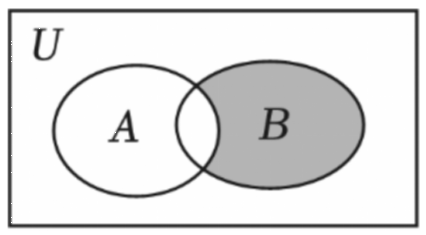
\includegraphics[width=0.26\textwidth]{figures/gao76_q14_venn.png}
\end{center}

\keepwithprev
A. $\{x\mid-2\leqslant x<4\}$\qquad B. $\{x\mid-1\leqslant x\leqslant3\}$

C. $\{x\mid x\leqslant3\text{ 或 }x\geqslant4\}$\qquad D. $\{x\mid-2\leqslant x\leqslant4\}$

\ifanswer
\solbegin
\step{全集 $U=\R$，集合 $A=\{x\mid x<-1\text{ 或 }x>4\}$，}
\step{$B=\{x\mid x^2-x-6\leqslant0\}=\{x\mid-2\leqslant x\leqslant3\}$，故 $A\cap B=\{x\mid-2\leqslant x<-1\}$，}
\step{故阴影部分表示的集合为 $\overline{A\cap B}=\{x\mid-1\leqslant x\leqslant3\}$. 故选 $B$.}
\solend
\fi

\item 设 $a$、$b$、$c\in\R$，给出下列命题：①若 $a>b$，则 $a^2>b^2$，②“$a>b$”是“$a^3>b^3$”的充要条件，③若 $a^2>b^2$，则 $|a|>|b|$，④若 $\dfrac ab>1$，则 $a>b$，⑤若 $a>b$，$c\neq0$，则 $\dfrac a{c^2}>\dfrac b{c^2}$，其中真命题的个数是\mbox{（\quad）}

\keepwithprev
A. $1$ 个\qquad B. $2$ 个\qquad C. $3$ 个\qquad D. $4$ 个

\ifanswer
\solbegin
\step{对于①，取 $a=2$，$b=-2$，满足 $a>b$，而 $a^2=b^2$，故为假命题；}
\step{对于②，$a>b\Leftrightarrow a^3-b^3=(a-b)(a^2+ab+b^2)=(a-b)\left[\left(a+\dfrac12b\right)^2+\dfrac34b^2\right]>0$}
\step{$\Leftrightarrow a^3>b^3$，故为真命题；}
\step{对于③，$a^2>b^2\Leftrightarrow|a|^2>|b|^2\Leftrightarrow|a|>|b|$，故为真命题；}
\step{对于④，取 $a=-2$，$b=-1$，满足 $\dfrac ab>1$，而 $a<b$，故为假命题；}
\step{对于⑤，由题意得 $c^2>0$，由 $a>b$，则 $\dfrac a{c^2}>\dfrac b{c^2}$，故为真命题.}
\step{故选 $C$.}
\solend
\fi

\item 已知关于 $x$ 的两个一元二次不等式 $a_1x^2+b_1x+c_1>0$，$a_2x^2+b_2x+c_2>0$ 的解集分别为 $A$、$B$，其中 $a_i$、$b_i$、$c_i(i=1,2)$ 为常数且不为零，则“$\dfrac{a_1}{a_2}=\dfrac{b_1}{b_2}=\dfrac{c_1}{c_2}$”是“$A=B$”\mbox{（\quad）}

\keepwithprev
A. 充分不必要条件\qquad B. 必要不充分条件

C. 充要条件\qquad D. 既不充分也不必要条件

\ifanswer
\solbegin
\step{设 $\dfrac{a_1}{a_2}=\dfrac{b_1}{b_2}=\dfrac{c_1}{c_2}=\lambda$，}
\step{①当 $\lambda>0$ 时，则 $a_1=\lambda a_2$，$b_1=\lambda b_2$，$c_1=\lambda c_2$，}
\step{$a_1x^2+b_1x+c_1>0\Leftrightarrow\lambda a_2x^2+\lambda b_2x+\lambda c_2>0\Leftrightarrow a_2x^2+b_2x+c_2>0$，}
\step{所以 $A=B$，}
\step{②当 $\lambda<0$ 时，则 $a_1=\lambda a_2$，$b_1=\lambda b_2$，$c_1=\lambda c_2$，}
\step{$a_1x^2+b_1x+c_1>0\Leftrightarrow\lambda a_2x^2+\lambda b_2x+\lambda c_2>0\Leftrightarrow a_2x^2+b_2x+c_2<0$，}
\step{所以 $A\neq B$，充分性不成立，}
\step{当 $A=B=\R$ 时，则 $\Delta<0$ 且 $a_1$、$a_2>0$，$\dfrac{a_1}{a_2}=\dfrac{b_1}{b_2}=\dfrac{c_1}{c_2}$ 不一定成立，}
\step{必要性不成立.}
\step{所以 $\dfrac{a_1}{a_2}=\dfrac{b_1}{b_2}=\dfrac{c_1}{c_2}$ 是 $A=B$ 的既不充分也不必要条件，故选 $D$.}
\solend
\fi

\end{enumerate}

\bigsec{三、解答题}

\begin{enumerate}
\setcounter{enumi}{16}

\item 求下列关于 $x$ 的不等式（组）的解集.

（1）$\begin{cases}9x^2-6x-24>0\\ \dfrac{x+3}{x-1}>2\end{cases}$；

（2）$|2x+1|-|2-x|>2$.

\ifanswer
\solbegin
\stepm{(1)}{不等式 $\dfrac{x+3}{x-1}>2$ 可化为 $\dfrac{x+3}{x-1}-2>0$，}
\step{即 $\dfrac{-x+5}{x-1}>0$，即 $(x-1)(x-5)<0$，解得 $1<x<5$，}
\step{不等式 $9x^2-6x-24>0$ 可化为 $(3x+4)(x-2)>0$，}
\step{解得 $x<-\dfrac43$ 或 $x>2$，}
\step{所以不等式的解集为 $(2,5)$.}
\stepm{(2)}{当 $x\leqslant-\dfrac12$ 时，$|2x+1|-|2-x|>2$ 等价于 $-2x-1-(2-x)>2$，}
\step{解得 $x<-5$，所以 $x<-5$，}
\step{当 $-\dfrac12<x<2$ 时，$|2x+1|-|2-x|>2$ 等价于 $2x+1-(2-x)>2$，}
\step{解得 $x>1$，所以 $1<x<2$，}
\step{当 $x\geqslant2$ 时，$|2x+1|-|2-x|>2$ 等价于 $2x+1-(x-2)>2$，}
\step{解得 $x>-1$，所以 $x\geqslant2$，}
\step{综上，$|2x+1|-|2-x|>2$ 的解集为 $(-\infty,-5)\cup(1,+\infty)$.}
\solend
\fi

\ansspace

\item 设 $m$ 为实数，求关于 $x$ 与 $y$ 的二元一次方程组 $\begin{cases}y=x+m\\ mx-y=4\end{cases}$ 的解集.

\ifanswer
\solbegin
\step{消去 $y$ 得 $(m-1)x=m+4$，}
\step{当 $m-1=0$，即 $m=1$ 时，$0=5$ 不成立，则 $x$ 无解，原方程组的解集为 $\varnothing$；}
\step{当 $m-1\neq0$，即 $m\neq1$ 时，则 $x=\dfrac{m+4}{m-1}$，$y=\dfrac{m+4}{m-1}+m=\dfrac{m^2+4}{m-1}$，}
\step{原方程组的解集为 $\left\{\left(\dfrac{m+4}{m-1},\dfrac{m^2+4}{m-1}\right)\right\}$.}
\step{综上所述，当 $m=1$ 时，方程组的解集为 $\varnothing$；}
\step{当 $m\neq1$ 时，方程组的解集为 $\left\{\left(\dfrac{m+4}{m-1},\dfrac{m^2+4}{m-1}\right)\right\}$.}
\solend
\fi

\ansspace

\item 已知集合 $A=\{x\mid-2\leqslant x-1\leqslant5\}$，集合 $B=\{x\mid m+1\leqslant x\leqslant2m-1\}(m\in\R)$.

（1）若 $m=4$，全集 $U=\R$，求 $A\cap B$；

（2）设命题 $p:x\in A$；命题 $q:x\in B$，若命题 $p$ 是命题 $q$ 的必要不充分条件，求实数 $m$ 的取值范围.

\ifanswer
\solbegin
\stepm{(1)}{由题意得 $A=\{x\mid-2\leqslant x-1\leqslant5\}=\{x\mid-1\leqslant x\leqslant6\}$，}
\step{当 $m=4$ 时，$B=\{x\mid5\leqslant x\leqslant7\}$，$A\cap B=\{x\mid5\leqslant x\leqslant6\}$；}
\stepm{(2)}{因为命题 $p$ 是命题 $q$ 的必要不充分条件，所以集合 $B$ 是集合 $A$ 的真子集，}
\step{当 $B=\varnothing$ 时，$m+1>2m-1$，解得 $m<2$，}
\step{当 $B\neq\varnothing$ 时，$\begin{cases}m+1\leqslant2m-1\\ m+1\geqslant-1\\ 2m-1\leqslant6\end{cases}$（等号不能同时成立），解得 $2\leqslant m\leqslant\dfrac72$，}
\step{综上所述，实数 $m$ 的取值范围为 $\left(-\infty,\dfrac72\right]$.}
\solend
\fi

\ansspace

\item （1）已知实数 $x\neq0$，求 $x+\dfrac1x$ 的取值范围；

（2）如图，要设计一张矩形海报，该海报含有大小相等的左右两个矩形栏目（即图中阴影部分），这两栏的面积之和为 $18000\,\mathrm{cm}^2$，四周空白的宽度为 $10\,\mathrm{cm}$，两栏之间的中缝空白的宽度为 $16\,\mathrm{cm}$，怎样确定海报的高与宽的尺寸（单位：$\mathrm{cm}$），能使矩形海报面积 $S$ 最小？最小面积是多少？

\begin{center}
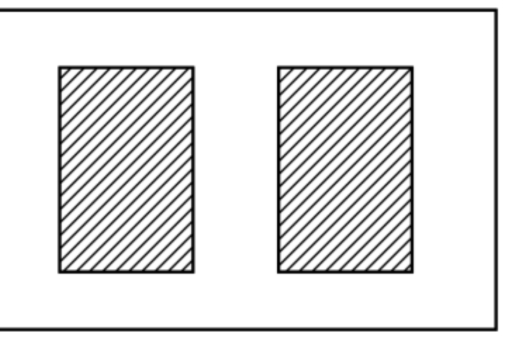
\includegraphics[width=0.34\textwidth]{figures/gao76_q20_poster.png}
\end{center}

\ifanswer
\solbegin
\stepm{(1)}{当 $x>0$ 时，$x+\dfrac1x\geqslant2\sqrt{x\times\dfrac1x}=2$，当且仅当 $x=\dfrac1x$，即 $x=1$ 取等号，}
\step{当 $x<0$ 时，$-x-\dfrac1x\geqslant2\sqrt{(-x)\times\dfrac1{-x}}=2$，所以 $x+\dfrac1x\leqslant-2$，}
\step{当且仅当 $-x=-\dfrac1x$，即 $x=-1$ 取等号，}
\step{综上所述，$x+\dfrac1x$ 的取值范围为 $(-\infty,-2]\cup[2,+\infty)$.}
\stepm{(2)}{设矩形栏目宽为 $x$，高为 $y$，则 $2xy=18000$，}
\step{所以 $S=(2x+36)(y+20)=2xy+36y+40x+720$}
% 原卷此行把 18720 写作 36720，照录（见文件头“原卷笔误/存疑”①）
\step{$=18000+36y+40x+720\geqslant18720+2\sqrt{36y\times40x}$}
\step{$=36720+2\sqrt{36\times40\times18000}=18720+7200=25920$，}
\step{当且仅当 $36y=40x$，即 $x=90$，$y=100$ 取等号，}
\step{所以海报的高为 $120\,\mathrm{cm}$ 与宽为 $216\,\mathrm{cm}$，可使矩形海报面积 $S$ 最小，}
\step{最小面积为 $25920$.}
\solend
\fi

\ansspace

\item 若实数 $x$、$y$、$m$ 满足 $|x-m|>|y-m|$，则称 $x$ 比 $y$ 远离 $m$.

（1）$0$ 比 $\dfrac12$ 远离 $2$ 吗？说明理由；

（2）若 $\dfrac1{2x-1}$ 比 $\dfrac12$ 远离 $1$，求实数 $x$ 的取值范围；

（3）若 $m\leqslant1$，$x+y=2$，试问：$x$ 与 $x^2+y^2$ 哪一个更远离 $m$，并说明理由.

\ifanswer
\solbegin
\stepm{(1)}{$0$ 比 $\dfrac12$ 远离 $2$，理由为：}
\step{由于 $|0-2|=2>\dfrac32=\left|\dfrac12-2\right|$，所以 $0$ 比 $\dfrac12$ 远离 $2$.}
\stepm{(2)}{由 $\dfrac1{2x-1}$ 比 $\dfrac12$ 远离 $1$，得 $\left|\dfrac1{2x-1}-1\right|>\left|\dfrac12-1\right|$，即 $\left|\dfrac1{2x-1}-1\right|>\dfrac12$，}
\step{则 $\dfrac1{2x-1}-1>\dfrac12$ 或 $\dfrac1{2x-1}-1<-\dfrac12$，整理得 $\dfrac1{2x-1}>\dfrac32$ 或 $\dfrac1{2x-1}<\dfrac12$，}
\step{因此 $0<2x-1<\dfrac23$ 或 $2x-1<0$ 或 $2x-1>2$，}
\step{解得 $\dfrac12<x<\dfrac56$ 或 $x<\dfrac12$ 或 $x>\dfrac32$，}
\step{所以 $x$ 的取值范围是 $\left(-\infty,\dfrac12\right)\cup\left(\dfrac12,\dfrac56\right)\cup\left(\dfrac32,+\infty\right)$.}
\stepm{(3)}{$x^2+y^2$ 比 $x$ 更远离 $m$，理由为：}
\step{由 $x^2+y^2\geqslant\dfrac{(x+y)^2}2=2\geqslant m$，得 $|x^2+y^2-m|=x^2+y^2-m$，}
\step{由 $x+y=2$，得 $x^2+y^2=x^2+(2-x)^2=2x^2-4x+4$，}
\step{于是 $|x^2+y^2-m|-|x-m|=2x^2-4x+4-m-|x-m|$，}
\step{当 $x\geqslant m$ 时，$|x^2+y^2-m|-|x-m|=2x^2-4x+4-m-(x-m)$}
\step{$=2\left(x-\dfrac54\right)^2+\dfrac78>0$，即 $|x^2+y^2-m|>|x-m|$；}
\step{当 $x<m$ 时，$|x^2+y^2-m|-|x-m|=2x^2-4x+4-m+(x-m)$}
\step{$=2\left(x-\dfrac34\right)^2+\dfrac{23}8-2m$，}
\step{由 $m\leqslant1$，得 $\dfrac{23}8-2m>0$，因此 $2\left(x-\dfrac34\right)^2+\dfrac{23}8-2m>0$，}
\step{即 $|x^2+y^2-m|>|x-m|$，}
\step{所以 $|x^2+y^2-m|>|x-m|$，即 $x^2+y^2$ 比 $x$ 更远离 $m$.}
\solend
\fi

\ansspace*[7]

\end{enumerate}

\end{document}
"
% 紧凑版：xelatex "\def\iscompact{1}% 高一76_六十中学_10月月考.tex
%   —— 高一上数学“2026-2027 年六十中学高一上 10 月月考”（讲评版）
% 试卷版：xelatex 高一76_六十中学_10月月考.tex
% 答案版：xelatex "\def\isanswer{1}\input{高一76_六十中学_10月月考.tex}"
% 紧凑版：xelatex "\def\iscompact{1}\input{高一76_六十中学_10月月考.tex}"
%
% 原始材料：微信公众号“魔都数学加油站”文章，连载“27学年高一76”；
% 原文标题“27学年高一76——2026-2027年上海市六十中学高一上10月月考”；
% 原文链接：https://mp.weixin.qq.com/s/GrKZjQrV1Xb0wy0BUuzAHw。
% 页面标注发布时间 2026-10-22 21:45（上海）。
% 正文为 10 张 PNG 页（`原图/高一76_六十中学_10月月考/01..10.png`）：
% 第 4、5、8、9 页为 4762×6735，其余 6 页为 2560×3620，均按页序读取。
% 10 页全为试卷正文页（卷首标题在第 1 页页顶，卷末第 21 题 (3) 解析止于第 10 页），
% 无封面页、目录页、二维码或宣传页。粉色斜排“魔都数学加油站”为卷面水印，未录入。
%
% 卷首标题：照卷面印作“2026-2027 年六十中学高一上 10 月月考”（黑体加粗一行）。
% 原卷年份区间用半角连字符，本稿按全稿惯例排 en dash；原卷无副标题。
%
% 篇幅与题号：原卷自第 3 题起编号（第 1、2 题不在本卷内）。填空题 3—12（10 题）、
% 选择题 13—16（4 题）、解答题 17—21（5 题），共 19 题。本稿沿用原节与原题号，
% 只改排为全稿统一的大节样式。
%
% 讲评版：原卷第 3、5 题只印【答案】（“$(0,1)$”“$a$、$b$ 都不能被 $3$ 整除”），
% 本稿只给 \ans{}；其余 17 题均印【解析】，用 \solbegin…\solend。四道选择题的作答
% 括号原卷即留空，答案写在解析末句“故选 C／B／C／D”，照录在解析内，不另提 \ans{}。
%
% 副标题：原卷未印副标题。本稿按“知识模块”口径标作“集合与常用逻辑用语、不等式”：
% 19 题中集合与常用逻辑用语 6 题（第 5、12、14、16、19 题及第 4 题的恒等变形），
% 不等式 13 题（第 3、6—11、13、15、17、18、20、21 题），两类均确有分量，故并标。
% 口径同 高一63、高一68—75。
%
% 与原卷的排版差异：
%   ① 原卷每题下直接印【答案】/【解析】，本稿按全稿惯例将答案与解析置于答案版；
%   ② 原卷未印副标题，本稿按“知识模块”口径补出；
%   ③ 原卷填空横线约四个字宽，本稿按全稿惯例统一排 \blankline[4.4em]；
%   ④ 原卷数集记号排斜体 $R$、$N$（第 4、6、7、8、11、12、14、15、19、20 题），本稿
%      按全稿惯例改用 $\R$、$\N$（同 高一68—75）；第 7、19、20 题的“解集为 $\R$”同此；
%   ⑤ 原卷句末标点多为西文句点，均逐处照录；
%   ⑥ 第 17—21 题的子问原卷印作“（1）…（2）…”，本稿按 高一69—75 成例用行内
%      “（1）（2）（3）”段，解析中的子问标号用 \stepm{(1)}{…}；
%   ⑦ 每道解答题原卷未留作答空白，本稿按全稿惯例加 \ansspace（末题用 \ansspace*）；
%   ⑧ 选择题的作答括号原卷排半角“(    )”，本稿按全稿惯例排 \mbox{（\quad）}；
%      选项行排照原卷——第 13、14、15、16 题一行两条、分两行排（本稿按原卷分行）；
%   ⑨ 第 10、11、17—21 题解析中的不等式组／方程组，原卷均排作“{”连接的多行式，
%      本稿按全稿惯例排 cases；
%   ⑩ 第 14 题题干右侧有一幅韦恩图（全集矩形内含 A、B 两圆，B 涂灰）：本稿按原卷
%      截图裁取（`figures/gao76_q14_venn.png`，由第 5 页原图裁出、去除粉色水印后转
%      灰度，未放大），放在题干之后、选项之前，仅答案版出；
%   ⑪ 第 20 题 (2) 题干右侧有一幅示意图（大矩形内两个斜线阴影小矩形）：本稿按原卷
%      截图裁取（`figures/gao76_q20_poster.png`，由第 8 页原图裁出、去除粉色水印后转
%      灰度，未放大），放在该小题文字之后，仅答案版出。
%
% 原卷笔误/存疑（均照录未改，正文对应处另有 % 注）：
%   ① 第 20 题 (2) 解析第 3 行把 $2xy+720$ 写成 $36720$（实为 $18000+720=18720$），
%      同式下一行又写回 $18720$，前后不一致；原卷如此，照录未改。
%   ② 第 14 题的韦恩图阴影是把整个 $B$ 圆（含 $A\cap B$ 部分）涂灰，而解析按
%      $\overline{A\cap B}$ 求解，二者不一致；原卷图文如此，照录未改。
%
% 行数核对：逐题数 \step/\stepm 条数与原卷【解析】印刷行数，17 题逐一相符，
% 合计 118 条 / 118 行（Q4：3；Q6：4；Q7：1；Q8：6；Q9：3；Q10：7；Q11：4；
% Q12：16；Q13：1；Q14：3；Q15：7；Q16：10；Q17：12；Q18：6；Q19：6；Q20：11；
% Q21：18）。另第 3、5 题只印【答案】，各提 \ans{}，不计入 \step 账。
%
% 插图：第 14 题题干的韦恩图、第 20 题 (2) 的示意图，见上⑩⑪；其余题干无配图。
%
\documentclass[a4paper,11pt]{article}
\usepackage{common}

\begin{document}

\examtitlest[3]{2026--2027 年六十中学高一上 10 月月考}{集合与常用逻辑用语、不等式}

\bigsec{一、填空题}

\begin{enumerate}
\setcounter{enumi}{2}

\item 不等式 $\dfrac{x}{1-x}>0$ 的解集是\blankline[4.4em].

\ifanswer
\ans{$(0,1)$}
\fi

\item 已知 $2x^2+x+1=a(x+1)^2+b(x+1)+2$，对 $x\in\R$ 恒成立，$ab=$\blankline[4.4em].

\ifanswer
\solbegin
\step{若 $2x^2+x+1=a(x+1)^2+b(x+1)+2$ 对 $x\in\R$ 恒成立，}
\step{即 $2x^2+x+1=ax^2+(2a+b)x+a+b+2$ 对 $x\in\R$ 恒成立，}
\step{必有 $\begin{cases}a=2\\ 2a+b=1\\ a+b+2=1\end{cases}$，解得 $a=2$，$b=-3$，所以 $ab=-6$.}
\solend
\fi

\item 利用反证法证明命题：“如果 $a$、$b\in\N$，$ab$ 可被 $3$ 整除，那么 $a$、$b$ 中至少有一个能被 $3$ 整除”时，假设的内容应是\blankline[4.4em].

\ifanswer
\ans{$a$、$b$ 都不能被 $3$ 整除}
\fi

\item 已知 $x\in\R$，方程 $|x+1|+|2-x|=3$ 的解集为\blankline[4.4em].

\ifanswer
\solbegin
\step{当 $x<-1$ 时，则 $|x+1|+|2-x|=-x-1+2-x=1-2x>3$；}
\step{当 $-1\leqslant x\leqslant2$ 时，则 $|x+1|+|2-x|=x+1+2-x=3$；}
\step{当 $x>2$ 时，则 $|x+1|+|2-x|=x+1+x-2=2x-1>3$.}
\step{综上所述，原方程的解集为 $[-1,2]$.}
\solend
\fi

\item 若关于 $x$ 的不等式 $x^2+kx+1\geqslant0$ 的解集为 $\R$，则实数 $k$ 的取值范围是\blankline[4.4em].

\ifanswer
\solbegin
\step{$\Delta=k^2-4\leqslant0\Rightarrow-2\leqslant k\leqslant2$，所以实数 $k$ 的取值范围是 $[-2,2]$.}
\solend
\fi

\item 已知 $a$、$b\in\R$，且 $ab>0$，则下列不等式中，恒成立的序号是\blankline[4.4em].

① $a^2+b^2>2ab$；② $a+b\geqslant2\sqrt{ab}$；③ $\dfrac1a+\dfrac1b>\dfrac2{\sqrt{ab}}$；④ $\dfrac ba+\dfrac ab\geqslant2$.

\ifanswer
\solbegin
\step{因为 $a^2+b^2\geqslant2ab$ 对于 $a$、$b\in\R$ 恒成立，当且仅当 $a=b$ 时取等号，}
\step{所以①错误；}
\step{对于②，③，显然 $a<0$，$b<0$ 时，不等式均不成立，即②和③错误；}
\step{对于④，因为 $ab>0$，所以 $\dfrac ba>0,\dfrac ab>0$，}
\step{由基本不等式得 $\dfrac ba+\dfrac ab\geqslant2\sqrt{\dfrac ba\cdot\dfrac ab}=2$，即④正确.}
\step{故正确的是④.}
\solend
\fi

\item 已知正实数 $m$、$n$ 满足 $m+\dfrac2n=1$，则 $\dfrac1m+2n$ 的最小值为\blankline[4.4em].

\ifanswer
\solbegin
\step{$\dfrac1m+2n=\left(m+\dfrac2n\right)\left(\dfrac1m+2n\right)=5+2mn+\dfrac2{mn}$，}
\step{因为 $mn>0$，所以 $2mn+\dfrac2{mn}\geqslant2\sqrt{2mn\cdot\dfrac2{mn}}=4$，}
\step{当且仅当 $2mn=\dfrac2{mn}$，即 $m=\dfrac13$，$n=3$ 时取等号，所以 $\dfrac1m+2n$ 的最小值为 $9$.}
\solend
\fi

\item 若关于 $x$ 的不等式组 $\begin{cases}3x+1>0\\ x+\dfrac1a\leqslant2\end{cases}$ 恰好有两个整数解，则实数 $a$ 的取值范围为\blankline[4.4em].

\ifanswer
\solbegin
\step{由 $3x+1>0$ 得 $x>-\dfrac13$；若 $a<0$，则 $\dfrac1a<0$，由 $x+\dfrac1a\leqslant2$ 得 $x\leqslant2-\dfrac1a>2$，}
\step{则解集 $\left(-\dfrac13,2-\dfrac1a\right]$ 必同时含有整数 $0$、$1$、$2$，不合题意；}
\step{又 $a=0$ 使 $\dfrac1a$ 无意义，故 $a>0$；}
\step{此时原不等式组的解集为 $\left(-\dfrac13,2-\dfrac1a\right]$，}
\step{其中大于 $-\dfrac13$ 的整数依次为 $0$，$1$，$2$，$\cdots$，}
\step{恰有两个整数解即解集只含 $0$ 与 $1$，故 $1\leqslant2-\dfrac1a<2$，即 $\dfrac1a\leqslant1$ 且 $\dfrac1a>0$，}
\step{结合 $a>0$，解得 $a\geqslant1$.}
\solend
\fi

\item 已知 $a\in\R$，若关于 $x$ 的方程 $x^2+ax+a^2-8=0$ 有两个实根 $x_1$、$x_2$，且 $\dfrac1{x_1}+\dfrac1{x_2}=-\dfrac12$，则 $a$ 的值为\blankline[4.4em].

\ifanswer
\solbegin
\step{由题意得 $\Delta=a^2-4(a^2-8)=32-3a^2\geqslant0$，解得 $a^2\leqslant\dfrac{32}3$，}
\step{由韦达定理得 $x_1+x_2=-a$，$x_1x_2=a^2-8$，}
\step{则 $\dfrac1{x_1}+\dfrac1{x_2}=\dfrac{x_1+x_2}{x_1x_2}=\dfrac{-a}{a^2-8}=-\dfrac12$，即 $a^2-2a-8=(a-4)(a+2)=0$，}
\step{解得 $a=4$ 或 $a=-2$，又 $a^2\leqslant\dfrac{32}3$，则 $a=-2$.}
\solend
\fi

\item 已知有限集 $A=\{a_1,a_2,\cdots,a_n\}(n\geqslant2,n\in\N)$，若 $A$ 中元素 $a_i(i=1,2,\cdots,n)$ 满足 $a_1+a_2+\cdots+a_n=a_1\times a_2\times\cdots\times a_n$，就称 $A$ 为“完美集”，以下四个命题：

①集合 $\{-1-\sqrt3,-1+\sqrt3\}$ 不是“完美集”；

②若 $a_1$、$a_2$ 是两个不同的正数，且 $\{a_1,a_2\}$ 是“完美集”，则 $a_1$、$a_2$ 至少有一个大于 $2$；

③二元“完美集”有无穷多个；

④若 $a_i$ 均为正整数，则“完美集”$A$ 有且只有一个，且 $n=3$.

其中，真命题的序号是\blankline[4.4em].

\ifanswer
\solbegin
\step{对于①选项：$(-1-\sqrt3)+(-1+\sqrt3)=-2$，$(-1-\sqrt3)\times(-1+\sqrt3)=-2$，}
\step{故 $(-1-\sqrt3)+(-1+\sqrt3)=(-1-\sqrt3)\times(-1+\sqrt3)$，}
\step{所以集合 $\{-1-\sqrt3,-1+\sqrt3\}$ 是“完美集”，故①错误；}
\step{对于②选项：集合 $\{a_1,a_2\}$ 是“完美集”，设 $a_1+a_2=a_1a_2=t>0$，}
\step{则 $a_1$、$a_2$ 可以看成一元二次方程 $x^2-tx+t=0$ 的两正根，则 $\Delta=t^2-4t>0$，}
\step{解得 $t<0$（舍）或 $t>4$，即 $a_1a_2>4$，所以至少有一个大于 $2$，故②正确；}
\step{对于③选项：由②得一元二次方程 $x^2-tx+t=0$ 当 $t$ 取不同值时，}
\step{$a_1$、$a_2$ 的值是不同的，因而二元“完美集”有无穷多个，故③正确；}
\step{对于④选项：设 $a_1<a_2<a_3<\cdots<a_n$，}
\step{则 $a_1\times a_2\times\cdots\times a_n=a_1+a_2+\cdots+a_n<na_n$，}
\step{所以 $a_1\times a_2\times\cdots\times a_{n-1}<n$，又 $a_i\in\N^*$，所以 $n\leqslant3$，}
\step{当 $n=2$ 时，$a_1<2$，则 $a_1=1$，$a_1a_2\neq a_1+a_2$，不合题意，}
\step{当 $n=3$ 时，$a_1a_2<3$，所以只能是 $a_1=1$，$a_2=2$，}
\step{由 $a_1+a_2+a_3=a_1a_2a_3$，代入解得 $a_3=3$，所以此时“完美集”只有一个，}
\step{为 $\{1,2,3\}$，故④正确.}
\step{故正确的是②③④.}
\solend
\fi

\end{enumerate}

\bigsec{二、选择题}

\begin{enumerate}
\setcounter{enumi}{12}

\item 已知 $x$、$y\in\R$，则“$xy\geqslant0$”是“$xy=|xy|$”的\mbox{（\quad）}

\keepwithprev
A. 充分非必要条件\qquad B. 必要非充分条件

C. 充要条件\qquad D. 既非充分也非必要条件

\ifanswer
\solbegin
\step{$xy\geqslant0\Leftrightarrow xy=|xy|$，故“$xy\geqslant0$”是“$xy=|xy|$”的充要条件. 故选 $C$.}
\solend
\fi

\needvspace{22\baselineskip}
\item 已知全集 $U=\R$，集合 $A=\{x\mid x<-1\text{ 或 }x>4\}$，$B=\{x\mid x^2-x-6\leqslant0\}$，则阴影部分表示的集合为\mbox{（\quad）}

\begin{center}
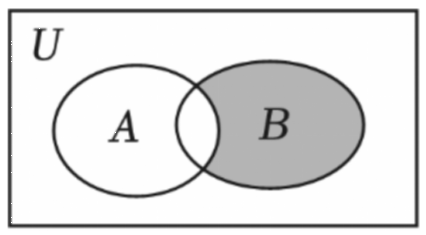
\includegraphics[width=0.26\textwidth]{figures/gao76_q14_venn.png}
\end{center}

\keepwithprev
A. $\{x\mid-2\leqslant x<4\}$\qquad B. $\{x\mid-1\leqslant x\leqslant3\}$

C. $\{x\mid x\leqslant3\text{ 或 }x\geqslant4\}$\qquad D. $\{x\mid-2\leqslant x\leqslant4\}$

\ifanswer
\solbegin
\step{全集 $U=\R$，集合 $A=\{x\mid x<-1\text{ 或 }x>4\}$，}
\step{$B=\{x\mid x^2-x-6\leqslant0\}=\{x\mid-2\leqslant x\leqslant3\}$，故 $A\cap B=\{x\mid-2\leqslant x<-1\}$，}
\step{故阴影部分表示的集合为 $\overline{A\cap B}=\{x\mid-1\leqslant x\leqslant3\}$. 故选 $B$.}
\solend
\fi

\item 设 $a$、$b$、$c\in\R$，给出下列命题：①若 $a>b$，则 $a^2>b^2$，②“$a>b$”是“$a^3>b^3$”的充要条件，③若 $a^2>b^2$，则 $|a|>|b|$，④若 $\dfrac ab>1$，则 $a>b$，⑤若 $a>b$，$c\neq0$，则 $\dfrac a{c^2}>\dfrac b{c^2}$，其中真命题的个数是\mbox{（\quad）}

\keepwithprev
A. $1$ 个\qquad B. $2$ 个\qquad C. $3$ 个\qquad D. $4$ 个

\ifanswer
\solbegin
\step{对于①，取 $a=2$，$b=-2$，满足 $a>b$，而 $a^2=b^2$，故为假命题；}
\step{对于②，$a>b\Leftrightarrow a^3-b^3=(a-b)(a^2+ab+b^2)=(a-b)\left[\left(a+\dfrac12b\right)^2+\dfrac34b^2\right]>0$}
\step{$\Leftrightarrow a^3>b^3$，故为真命题；}
\step{对于③，$a^2>b^2\Leftrightarrow|a|^2>|b|^2\Leftrightarrow|a|>|b|$，故为真命题；}
\step{对于④，取 $a=-2$，$b=-1$，满足 $\dfrac ab>1$，而 $a<b$，故为假命题；}
\step{对于⑤，由题意得 $c^2>0$，由 $a>b$，则 $\dfrac a{c^2}>\dfrac b{c^2}$，故为真命题.}
\step{故选 $C$.}
\solend
\fi

\item 已知关于 $x$ 的两个一元二次不等式 $a_1x^2+b_1x+c_1>0$，$a_2x^2+b_2x+c_2>0$ 的解集分别为 $A$、$B$，其中 $a_i$、$b_i$、$c_i(i=1,2)$ 为常数且不为零，则“$\dfrac{a_1}{a_2}=\dfrac{b_1}{b_2}=\dfrac{c_1}{c_2}$”是“$A=B$”\mbox{（\quad）}

\keepwithprev
A. 充分不必要条件\qquad B. 必要不充分条件

C. 充要条件\qquad D. 既不充分也不必要条件

\ifanswer
\solbegin
\step{设 $\dfrac{a_1}{a_2}=\dfrac{b_1}{b_2}=\dfrac{c_1}{c_2}=\lambda$，}
\step{①当 $\lambda>0$ 时，则 $a_1=\lambda a_2$，$b_1=\lambda b_2$，$c_1=\lambda c_2$，}
\step{$a_1x^2+b_1x+c_1>0\Leftrightarrow\lambda a_2x^2+\lambda b_2x+\lambda c_2>0\Leftrightarrow a_2x^2+b_2x+c_2>0$，}
\step{所以 $A=B$，}
\step{②当 $\lambda<0$ 时，则 $a_1=\lambda a_2$，$b_1=\lambda b_2$，$c_1=\lambda c_2$，}
\step{$a_1x^2+b_1x+c_1>0\Leftrightarrow\lambda a_2x^2+\lambda b_2x+\lambda c_2>0\Leftrightarrow a_2x^2+b_2x+c_2<0$，}
\step{所以 $A\neq B$，充分性不成立，}
\step{当 $A=B=\R$ 时，则 $\Delta<0$ 且 $a_1$、$a_2>0$，$\dfrac{a_1}{a_2}=\dfrac{b_1}{b_2}=\dfrac{c_1}{c_2}$ 不一定成立，}
\step{必要性不成立.}
\step{所以 $\dfrac{a_1}{a_2}=\dfrac{b_1}{b_2}=\dfrac{c_1}{c_2}$ 是 $A=B$ 的既不充分也不必要条件，故选 $D$.}
\solend
\fi

\end{enumerate}

\bigsec{三、解答题}

\begin{enumerate}
\setcounter{enumi}{16}

\item 求下列关于 $x$ 的不等式（组）的解集.

（1）$\begin{cases}9x^2-6x-24>0\\ \dfrac{x+3}{x-1}>2\end{cases}$；

（2）$|2x+1|-|2-x|>2$.

\ifanswer
\solbegin
\stepm{(1)}{不等式 $\dfrac{x+3}{x-1}>2$ 可化为 $\dfrac{x+3}{x-1}-2>0$，}
\step{即 $\dfrac{-x+5}{x-1}>0$，即 $(x-1)(x-5)<0$，解得 $1<x<5$，}
\step{不等式 $9x^2-6x-24>0$ 可化为 $(3x+4)(x-2)>0$，}
\step{解得 $x<-\dfrac43$ 或 $x>2$，}
\step{所以不等式的解集为 $(2,5)$.}
\stepm{(2)}{当 $x\leqslant-\dfrac12$ 时，$|2x+1|-|2-x|>2$ 等价于 $-2x-1-(2-x)>2$，}
\step{解得 $x<-5$，所以 $x<-5$，}
\step{当 $-\dfrac12<x<2$ 时，$|2x+1|-|2-x|>2$ 等价于 $2x+1-(2-x)>2$，}
\step{解得 $x>1$，所以 $1<x<2$，}
\step{当 $x\geqslant2$ 时，$|2x+1|-|2-x|>2$ 等价于 $2x+1-(x-2)>2$，}
\step{解得 $x>-1$，所以 $x\geqslant2$，}
\step{综上，$|2x+1|-|2-x|>2$ 的解集为 $(-\infty,-5)\cup(1,+\infty)$.}
\solend
\fi

\ansspace

\item 设 $m$ 为实数，求关于 $x$ 与 $y$ 的二元一次方程组 $\begin{cases}y=x+m\\ mx-y=4\end{cases}$ 的解集.

\ifanswer
\solbegin
\step{消去 $y$ 得 $(m-1)x=m+4$，}
\step{当 $m-1=0$，即 $m=1$ 时，$0=5$ 不成立，则 $x$ 无解，原方程组的解集为 $\varnothing$；}
\step{当 $m-1\neq0$，即 $m\neq1$ 时，则 $x=\dfrac{m+4}{m-1}$，$y=\dfrac{m+4}{m-1}+m=\dfrac{m^2+4}{m-1}$，}
\step{原方程组的解集为 $\left\{\left(\dfrac{m+4}{m-1},\dfrac{m^2+4}{m-1}\right)\right\}$.}
\step{综上所述，当 $m=1$ 时，方程组的解集为 $\varnothing$；}
\step{当 $m\neq1$ 时，方程组的解集为 $\left\{\left(\dfrac{m+4}{m-1},\dfrac{m^2+4}{m-1}\right)\right\}$.}
\solend
\fi

\ansspace

\item 已知集合 $A=\{x\mid-2\leqslant x-1\leqslant5\}$，集合 $B=\{x\mid m+1\leqslant x\leqslant2m-1\}(m\in\R)$.

（1）若 $m=4$，全集 $U=\R$，求 $A\cap B$；

（2）设命题 $p:x\in A$；命题 $q:x\in B$，若命题 $p$ 是命题 $q$ 的必要不充分条件，求实数 $m$ 的取值范围.

\ifanswer
\solbegin
\stepm{(1)}{由题意得 $A=\{x\mid-2\leqslant x-1\leqslant5\}=\{x\mid-1\leqslant x\leqslant6\}$，}
\step{当 $m=4$ 时，$B=\{x\mid5\leqslant x\leqslant7\}$，$A\cap B=\{x\mid5\leqslant x\leqslant6\}$；}
\stepm{(2)}{因为命题 $p$ 是命题 $q$ 的必要不充分条件，所以集合 $B$ 是集合 $A$ 的真子集，}
\step{当 $B=\varnothing$ 时，$m+1>2m-1$，解得 $m<2$，}
\step{当 $B\neq\varnothing$ 时，$\begin{cases}m+1\leqslant2m-1\\ m+1\geqslant-1\\ 2m-1\leqslant6\end{cases}$（等号不能同时成立），解得 $2\leqslant m\leqslant\dfrac72$，}
\step{综上所述，实数 $m$ 的取值范围为 $\left(-\infty,\dfrac72\right]$.}
\solend
\fi

\ansspace

\item （1）已知实数 $x\neq0$，求 $x+\dfrac1x$ 的取值范围；

（2）如图，要设计一张矩形海报，该海报含有大小相等的左右两个矩形栏目（即图中阴影部分），这两栏的面积之和为 $18000\,\mathrm{cm}^2$，四周空白的宽度为 $10\,\mathrm{cm}$，两栏之间的中缝空白的宽度为 $16\,\mathrm{cm}$，怎样确定海报的高与宽的尺寸（单位：$\mathrm{cm}$），能使矩形海报面积 $S$ 最小？最小面积是多少？

\begin{center}
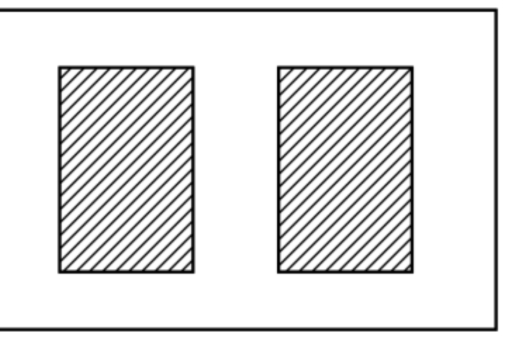
\includegraphics[width=0.34\textwidth]{figures/gao76_q20_poster.png}
\end{center}

\ifanswer
\solbegin
\stepm{(1)}{当 $x>0$ 时，$x+\dfrac1x\geqslant2\sqrt{x\times\dfrac1x}=2$，当且仅当 $x=\dfrac1x$，即 $x=1$ 取等号，}
\step{当 $x<0$ 时，$-x-\dfrac1x\geqslant2\sqrt{(-x)\times\dfrac1{-x}}=2$，所以 $x+\dfrac1x\leqslant-2$，}
\step{当且仅当 $-x=-\dfrac1x$，即 $x=-1$ 取等号，}
\step{综上所述，$x+\dfrac1x$ 的取值范围为 $(-\infty,-2]\cup[2,+\infty)$.}
\stepm{(2)}{设矩形栏目宽为 $x$，高为 $y$，则 $2xy=18000$，}
\step{所以 $S=(2x+36)(y+20)=2xy+36y+40x+720$}
% 原卷此行把 18720 写作 36720，照录（见文件头“原卷笔误/存疑”①）
\step{$=18000+36y+40x+720\geqslant18720+2\sqrt{36y\times40x}$}
\step{$=36720+2\sqrt{36\times40\times18000}=18720+7200=25920$，}
\step{当且仅当 $36y=40x$，即 $x=90$，$y=100$ 取等号，}
\step{所以海报的高为 $120\,\mathrm{cm}$ 与宽为 $216\,\mathrm{cm}$，可使矩形海报面积 $S$ 最小，}
\step{最小面积为 $25920$.}
\solend
\fi

\ansspace

\item 若实数 $x$、$y$、$m$ 满足 $|x-m|>|y-m|$，则称 $x$ 比 $y$ 远离 $m$.

（1）$0$ 比 $\dfrac12$ 远离 $2$ 吗？说明理由；

（2）若 $\dfrac1{2x-1}$ 比 $\dfrac12$ 远离 $1$，求实数 $x$ 的取值范围；

（3）若 $m\leqslant1$，$x+y=2$，试问：$x$ 与 $x^2+y^2$ 哪一个更远离 $m$，并说明理由.

\ifanswer
\solbegin
\stepm{(1)}{$0$ 比 $\dfrac12$ 远离 $2$，理由为：}
\step{由于 $|0-2|=2>\dfrac32=\left|\dfrac12-2\right|$，所以 $0$ 比 $\dfrac12$ 远离 $2$.}
\stepm{(2)}{由 $\dfrac1{2x-1}$ 比 $\dfrac12$ 远离 $1$，得 $\left|\dfrac1{2x-1}-1\right|>\left|\dfrac12-1\right|$，即 $\left|\dfrac1{2x-1}-1\right|>\dfrac12$，}
\step{则 $\dfrac1{2x-1}-1>\dfrac12$ 或 $\dfrac1{2x-1}-1<-\dfrac12$，整理得 $\dfrac1{2x-1}>\dfrac32$ 或 $\dfrac1{2x-1}<\dfrac12$，}
\step{因此 $0<2x-1<\dfrac23$ 或 $2x-1<0$ 或 $2x-1>2$，}
\step{解得 $\dfrac12<x<\dfrac56$ 或 $x<\dfrac12$ 或 $x>\dfrac32$，}
\step{所以 $x$ 的取值范围是 $\left(-\infty,\dfrac12\right)\cup\left(\dfrac12,\dfrac56\right)\cup\left(\dfrac32,+\infty\right)$.}
\stepm{(3)}{$x^2+y^2$ 比 $x$ 更远离 $m$，理由为：}
\step{由 $x^2+y^2\geqslant\dfrac{(x+y)^2}2=2\geqslant m$，得 $|x^2+y^2-m|=x^2+y^2-m$，}
\step{由 $x+y=2$，得 $x^2+y^2=x^2+(2-x)^2=2x^2-4x+4$，}
\step{于是 $|x^2+y^2-m|-|x-m|=2x^2-4x+4-m-|x-m|$，}
\step{当 $x\geqslant m$ 时，$|x^2+y^2-m|-|x-m|=2x^2-4x+4-m-(x-m)$}
\step{$=2\left(x-\dfrac54\right)^2+\dfrac78>0$，即 $|x^2+y^2-m|>|x-m|$；}
\step{当 $x<m$ 时，$|x^2+y^2-m|-|x-m|=2x^2-4x+4-m+(x-m)$}
\step{$=2\left(x-\dfrac34\right)^2+\dfrac{23}8-2m$，}
\step{由 $m\leqslant1$，得 $\dfrac{23}8-2m>0$，因此 $2\left(x-\dfrac34\right)^2+\dfrac{23}8-2m>0$，}
\step{即 $|x^2+y^2-m|>|x-m|$，}
\step{所以 $|x^2+y^2-m|>|x-m|$，即 $x^2+y^2$ 比 $x$ 更远离 $m$.}
\solend
\fi

\ansspace*[7]

\end{enumerate}

\end{document}
"
%
% 原始材料：微信公众号“魔都数学加油站”文章，连载“27学年高一76”；
% 原文标题“27学年高一76——2026-2027年上海市六十中学高一上10月月考”；
% 原文链接：https://mp.weixin.qq.com/s/GrKZjQrV1Xb0wy0BUuzAHw。
% 页面标注发布时间 2026-10-22 21:45（上海）。
% 正文为 10 张 PNG 页（`原图/高一76_六十中学_10月月考/01..10.png`）：
% 第 4、5、8、9 页为 4762×6735，其余 6 页为 2560×3620，均按页序读取。
% 10 页全为试卷正文页（卷首标题在第 1 页页顶，卷末第 21 题 (3) 解析止于第 10 页），
% 无封面页、目录页、二维码或宣传页。粉色斜排“魔都数学加油站”为卷面水印，未录入。
%
% 卷首标题：照卷面印作“2026-2027 年六十中学高一上 10 月月考”（黑体加粗一行）。
% 原卷年份区间用半角连字符，本稿按全稿惯例排 en dash；原卷无副标题。
%
% 篇幅与题号：原卷自第 3 题起编号（第 1、2 题不在本卷内）。填空题 3—12（10 题）、
% 选择题 13—16（4 题）、解答题 17—21（5 题），共 19 题。本稿沿用原节与原题号，
% 只改排为全稿统一的大节样式。
%
% 讲评版：原卷第 3、5 题只印【答案】（“$(0,1)$”“$a$、$b$ 都不能被 $3$ 整除”），
% 本稿只给 \ans{}；其余 17 题均印【解析】，用 \solbegin…\solend。四道选择题的作答
% 括号原卷即留空，答案写在解析末句“故选 C／B／C／D”，照录在解析内，不另提 \ans{}。
%
% 副标题：原卷未印副标题。本稿按“知识模块”口径标作“集合与常用逻辑用语、不等式”：
% 19 题中集合与常用逻辑用语 6 题（第 5、12、14、16、19 题及第 4 题的恒等变形），
% 不等式 13 题（第 3、6—11、13、15、17、18、20、21 题），两类均确有分量，故并标。
% 口径同 高一63、高一68—75。
%
% 与原卷的排版差异：
%   ① 原卷每题下直接印【答案】/【解析】，本稿按全稿惯例将答案与解析置于答案版；
%   ② 原卷未印副标题，本稿按“知识模块”口径补出；
%   ③ 原卷填空横线约四个字宽，本稿按全稿惯例统一排 \blankline[4.4em]；
%   ④ 原卷数集记号排斜体 $R$、$N$（第 4、6、7、8、11、12、14、15、19、20 题），本稿
%      按全稿惯例改用 $\R$、$\N$（同 高一68—75）；第 7、19、20 题的“解集为 $\R$”同此；
%   ⑤ 原卷句末标点多为西文句点，均逐处照录；
%   ⑥ 第 17—21 题的子问原卷印作“（1）…（2）…”，本稿按 高一69—75 成例用行内
%      “（1）（2）（3）”段，解析中的子问标号用 \stepm{(1)}{…}；
%   ⑦ 每道解答题原卷未留作答空白，本稿按全稿惯例加 \ansspace（末题用 \ansspace*）；
%   ⑧ 选择题的作答括号原卷排半角“(    )”，本稿按全稿惯例排 \mbox{（\quad）}；
%      选项行排照原卷——第 13、14、15、16 题一行两条、分两行排（本稿按原卷分行）；
%   ⑨ 第 10、11、17—21 题解析中的不等式组／方程组，原卷均排作“{”连接的多行式，
%      本稿按全稿惯例排 cases；
%   ⑩ 第 14 题题干右侧有一幅韦恩图（全集矩形内含 A、B 两圆，B 涂灰）：本稿按原卷
%      截图裁取（`figures/gao76_q14_venn.png`，由第 5 页原图裁出、去除粉色水印后转
%      灰度，未放大），放在题干之后、选项之前，仅答案版出；
%   ⑪ 第 20 题 (2) 题干右侧有一幅示意图（大矩形内两个斜线阴影小矩形）：本稿按原卷
%      截图裁取（`figures/gao76_q20_poster.png`，由第 8 页原图裁出、去除粉色水印后转
%      灰度，未放大），放在该小题文字之后，仅答案版出。
%
% 原卷笔误/存疑（均照录未改，正文对应处另有 % 注）：
%   ① 第 20 题 (2) 解析第 3 行把 $2xy+720$ 写成 $36720$（实为 $18000+720=18720$），
%      同式下一行又写回 $18720$，前后不一致；原卷如此，照录未改。
%   ② 第 14 题的韦恩图阴影是把整个 $B$ 圆（含 $A\cap B$ 部分）涂灰，而解析按
%      $\overline{A\cap B}$ 求解，二者不一致；原卷图文如此，照录未改。
%
% 行数核对：逐题数 \step/\stepm 条数与原卷【解析】印刷行数，17 题逐一相符，
% 合计 118 条 / 118 行（Q4：3；Q6：4；Q7：1；Q8：6；Q9：3；Q10：7；Q11：4；
% Q12：16；Q13：1；Q14：3；Q15：7；Q16：10；Q17：12；Q18：6；Q19：6；Q20：11；
% Q21：18）。另第 3、5 题只印【答案】，各提 \ans{}，不计入 \step 账。
%
% 插图：第 14 题题干的韦恩图、第 20 题 (2) 的示意图，见上⑩⑪；其余题干无配图。
%
\documentclass[a4paper,11pt]{article}
\usepackage{common}

\begin{document}

\examtitlest[3]{2026--2027 年六十中学高一上 10 月月考}{集合与常用逻辑用语、不等式}

\bigsec{一、填空题}

\begin{enumerate}
\setcounter{enumi}{2}

\item 不等式 $\dfrac{x}{1-x}>0$ 的解集是\blankline[4.4em].

\ifanswer
\ans{$(0,1)$}
\fi

\item 已知 $2x^2+x+1=a(x+1)^2+b(x+1)+2$，对 $x\in\R$ 恒成立，$ab=$\blankline[4.4em].

\ifanswer
\solbegin
\step{若 $2x^2+x+1=a(x+1)^2+b(x+1)+2$ 对 $x\in\R$ 恒成立，}
\step{即 $2x^2+x+1=ax^2+(2a+b)x+a+b+2$ 对 $x\in\R$ 恒成立，}
\step{必有 $\begin{cases}a=2\\ 2a+b=1\\ a+b+2=1\end{cases}$，解得 $a=2$，$b=-3$，所以 $ab=-6$.}
\solend
\fi

\item 利用反证法证明命题：“如果 $a$、$b\in\N$，$ab$ 可被 $3$ 整除，那么 $a$、$b$ 中至少有一个能被 $3$ 整除”时，假设的内容应是\blankline[4.4em].

\ifanswer
\ans{$a$、$b$ 都不能被 $3$ 整除}
\fi

\item 已知 $x\in\R$，方程 $|x+1|+|2-x|=3$ 的解集为\blankline[4.4em].

\ifanswer
\solbegin
\step{当 $x<-1$ 时，则 $|x+1|+|2-x|=-x-1+2-x=1-2x>3$；}
\step{当 $-1\leqslant x\leqslant2$ 时，则 $|x+1|+|2-x|=x+1+2-x=3$；}
\step{当 $x>2$ 时，则 $|x+1|+|2-x|=x+1+x-2=2x-1>3$.}
\step{综上所述，原方程的解集为 $[-1,2]$.}
\solend
\fi

\item 若关于 $x$ 的不等式 $x^2+kx+1\geqslant0$ 的解集为 $\R$，则实数 $k$ 的取值范围是\blankline[4.4em].

\ifanswer
\solbegin
\step{$\Delta=k^2-4\leqslant0\Rightarrow-2\leqslant k\leqslant2$，所以实数 $k$ 的取值范围是 $[-2,2]$.}
\solend
\fi

\item 已知 $a$、$b\in\R$，且 $ab>0$，则下列不等式中，恒成立的序号是\blankline[4.4em].

① $a^2+b^2>2ab$；② $a+b\geqslant2\sqrt{ab}$；③ $\dfrac1a+\dfrac1b>\dfrac2{\sqrt{ab}}$；④ $\dfrac ba+\dfrac ab\geqslant2$.

\ifanswer
\solbegin
\step{因为 $a^2+b^2\geqslant2ab$ 对于 $a$、$b\in\R$ 恒成立，当且仅当 $a=b$ 时取等号，}
\step{所以①错误；}
\step{对于②，③，显然 $a<0$，$b<0$ 时，不等式均不成立，即②和③错误；}
\step{对于④，因为 $ab>0$，所以 $\dfrac ba>0,\dfrac ab>0$，}
\step{由基本不等式得 $\dfrac ba+\dfrac ab\geqslant2\sqrt{\dfrac ba\cdot\dfrac ab}=2$，即④正确.}
\step{故正确的是④.}
\solend
\fi

\item 已知正实数 $m$、$n$ 满足 $m+\dfrac2n=1$，则 $\dfrac1m+2n$ 的最小值为\blankline[4.4em].

\ifanswer
\solbegin
\step{$\dfrac1m+2n=\left(m+\dfrac2n\right)\left(\dfrac1m+2n\right)=5+2mn+\dfrac2{mn}$，}
\step{因为 $mn>0$，所以 $2mn+\dfrac2{mn}\geqslant2\sqrt{2mn\cdot\dfrac2{mn}}=4$，}
\step{当且仅当 $2mn=\dfrac2{mn}$，即 $m=\dfrac13$，$n=3$ 时取等号，所以 $\dfrac1m+2n$ 的最小值为 $9$.}
\solend
\fi

\item 若关于 $x$ 的不等式组 $\begin{cases}3x+1>0\\ x+\dfrac1a\leqslant2\end{cases}$ 恰好有两个整数解，则实数 $a$ 的取值范围为\blankline[4.4em].

\ifanswer
\solbegin
\step{由 $3x+1>0$ 得 $x>-\dfrac13$；若 $a<0$，则 $\dfrac1a<0$，由 $x+\dfrac1a\leqslant2$ 得 $x\leqslant2-\dfrac1a>2$，}
\step{则解集 $\left(-\dfrac13,2-\dfrac1a\right]$ 必同时含有整数 $0$、$1$、$2$，不合题意；}
\step{又 $a=0$ 使 $\dfrac1a$ 无意义，故 $a>0$；}
\step{此时原不等式组的解集为 $\left(-\dfrac13,2-\dfrac1a\right]$，}
\step{其中大于 $-\dfrac13$ 的整数依次为 $0$，$1$，$2$，$\cdots$，}
\step{恰有两个整数解即解集只含 $0$ 与 $1$，故 $1\leqslant2-\dfrac1a<2$，即 $\dfrac1a\leqslant1$ 且 $\dfrac1a>0$，}
\step{结合 $a>0$，解得 $a\geqslant1$.}
\solend
\fi

\item 已知 $a\in\R$，若关于 $x$ 的方程 $x^2+ax+a^2-8=0$ 有两个实根 $x_1$、$x_2$，且 $\dfrac1{x_1}+\dfrac1{x_2}=-\dfrac12$，则 $a$ 的值为\blankline[4.4em].

\ifanswer
\solbegin
\step{由题意得 $\Delta=a^2-4(a^2-8)=32-3a^2\geqslant0$，解得 $a^2\leqslant\dfrac{32}3$，}
\step{由韦达定理得 $x_1+x_2=-a$，$x_1x_2=a^2-8$，}
\step{则 $\dfrac1{x_1}+\dfrac1{x_2}=\dfrac{x_1+x_2}{x_1x_2}=\dfrac{-a}{a^2-8}=-\dfrac12$，即 $a^2-2a-8=(a-4)(a+2)=0$，}
\step{解得 $a=4$ 或 $a=-2$，又 $a^2\leqslant\dfrac{32}3$，则 $a=-2$.}
\solend
\fi

\item 已知有限集 $A=\{a_1,a_2,\cdots,a_n\}(n\geqslant2,n\in\N)$，若 $A$ 中元素 $a_i(i=1,2,\cdots,n)$ 满足 $a_1+a_2+\cdots+a_n=a_1\times a_2\times\cdots\times a_n$，就称 $A$ 为“完美集”，以下四个命题：

①集合 $\{-1-\sqrt3,-1+\sqrt3\}$ 不是“完美集”；

②若 $a_1$、$a_2$ 是两个不同的正数，且 $\{a_1,a_2\}$ 是“完美集”，则 $a_1$、$a_2$ 至少有一个大于 $2$；

③二元“完美集”有无穷多个；

④若 $a_i$ 均为正整数，则“完美集”$A$ 有且只有一个，且 $n=3$.

其中，真命题的序号是\blankline[4.4em].

\ifanswer
\solbegin
\step{对于①选项：$(-1-\sqrt3)+(-1+\sqrt3)=-2$，$(-1-\sqrt3)\times(-1+\sqrt3)=-2$，}
\step{故 $(-1-\sqrt3)+(-1+\sqrt3)=(-1-\sqrt3)\times(-1+\sqrt3)$，}
\step{所以集合 $\{-1-\sqrt3,-1+\sqrt3\}$ 是“完美集”，故①错误；}
\step{对于②选项：集合 $\{a_1,a_2\}$ 是“完美集”，设 $a_1+a_2=a_1a_2=t>0$，}
\step{则 $a_1$、$a_2$ 可以看成一元二次方程 $x^2-tx+t=0$ 的两正根，则 $\Delta=t^2-4t>0$，}
\step{解得 $t<0$（舍）或 $t>4$，即 $a_1a_2>4$，所以至少有一个大于 $2$，故②正确；}
\step{对于③选项：由②得一元二次方程 $x^2-tx+t=0$ 当 $t$ 取不同值时，}
\step{$a_1$、$a_2$ 的值是不同的，因而二元“完美集”有无穷多个，故③正确；}
\step{对于④选项：设 $a_1<a_2<a_3<\cdots<a_n$，}
\step{则 $a_1\times a_2\times\cdots\times a_n=a_1+a_2+\cdots+a_n<na_n$，}
\step{所以 $a_1\times a_2\times\cdots\times a_{n-1}<n$，又 $a_i\in\N^*$，所以 $n\leqslant3$，}
\step{当 $n=2$ 时，$a_1<2$，则 $a_1=1$，$a_1a_2\neq a_1+a_2$，不合题意，}
\step{当 $n=3$ 时，$a_1a_2<3$，所以只能是 $a_1=1$，$a_2=2$，}
\step{由 $a_1+a_2+a_3=a_1a_2a_3$，代入解得 $a_3=3$，所以此时“完美集”只有一个，}
\step{为 $\{1,2,3\}$，故④正确.}
\step{故正确的是②③④.}
\solend
\fi

\end{enumerate}

\bigsec{二、选择题}

\begin{enumerate}
\setcounter{enumi}{12}

\item 已知 $x$、$y\in\R$，则“$xy\geqslant0$”是“$xy=|xy|$”的\mbox{（\quad）}

\keepwithprev
A. 充分非必要条件\qquad B. 必要非充分条件

C. 充要条件\qquad D. 既非充分也非必要条件

\ifanswer
\solbegin
\step{$xy\geqslant0\Leftrightarrow xy=|xy|$，故“$xy\geqslant0$”是“$xy=|xy|$”的充要条件. 故选 $C$.}
\solend
\fi

\needvspace{22\baselineskip}
\item 已知全集 $U=\R$，集合 $A=\{x\mid x<-1\text{ 或 }x>4\}$，$B=\{x\mid x^2-x-6\leqslant0\}$，则阴影部分表示的集合为\mbox{（\quad）}

\begin{center}
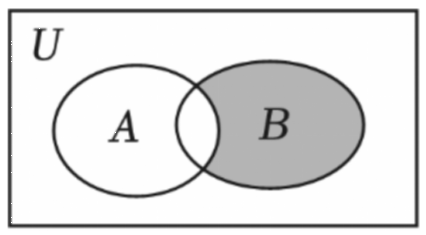
\includegraphics[width=0.26\textwidth]{figures/gao76_q14_venn.png}
\end{center}

\keepwithprev
A. $\{x\mid-2\leqslant x<4\}$\qquad B. $\{x\mid-1\leqslant x\leqslant3\}$

C. $\{x\mid x\leqslant3\text{ 或 }x\geqslant4\}$\qquad D. $\{x\mid-2\leqslant x\leqslant4\}$

\ifanswer
\solbegin
\step{全集 $U=\R$，集合 $A=\{x\mid x<-1\text{ 或 }x>4\}$，}
\step{$B=\{x\mid x^2-x-6\leqslant0\}=\{x\mid-2\leqslant x\leqslant3\}$，故 $A\cap B=\{x\mid-2\leqslant x<-1\}$，}
\step{故阴影部分表示的集合为 $\overline{A\cap B}=\{x\mid-1\leqslant x\leqslant3\}$. 故选 $B$.}
\solend
\fi

\item 设 $a$、$b$、$c\in\R$，给出下列命题：①若 $a>b$，则 $a^2>b^2$，②“$a>b$”是“$a^3>b^3$”的充要条件，③若 $a^2>b^2$，则 $|a|>|b|$，④若 $\dfrac ab>1$，则 $a>b$，⑤若 $a>b$，$c\neq0$，则 $\dfrac a{c^2}>\dfrac b{c^2}$，其中真命题的个数是\mbox{（\quad）}

\keepwithprev
A. $1$ 个\qquad B. $2$ 个\qquad C. $3$ 个\qquad D. $4$ 个

\ifanswer
\solbegin
\step{对于①，取 $a=2$，$b=-2$，满足 $a>b$，而 $a^2=b^2$，故为假命题；}
\step{对于②，$a>b\Leftrightarrow a^3-b^3=(a-b)(a^2+ab+b^2)=(a-b)\left[\left(a+\dfrac12b\right)^2+\dfrac34b^2\right]>0$}
\step{$\Leftrightarrow a^3>b^3$，故为真命题；}
\step{对于③，$a^2>b^2\Leftrightarrow|a|^2>|b|^2\Leftrightarrow|a|>|b|$，故为真命题；}
\step{对于④，取 $a=-2$，$b=-1$，满足 $\dfrac ab>1$，而 $a<b$，故为假命题；}
\step{对于⑤，由题意得 $c^2>0$，由 $a>b$，则 $\dfrac a{c^2}>\dfrac b{c^2}$，故为真命题.}
\step{故选 $C$.}
\solend
\fi

\item 已知关于 $x$ 的两个一元二次不等式 $a_1x^2+b_1x+c_1>0$，$a_2x^2+b_2x+c_2>0$ 的解集分别为 $A$、$B$，其中 $a_i$、$b_i$、$c_i(i=1,2)$ 为常数且不为零，则“$\dfrac{a_1}{a_2}=\dfrac{b_1}{b_2}=\dfrac{c_1}{c_2}$”是“$A=B$”\mbox{（\quad）}

\keepwithprev
A. 充分不必要条件\qquad B. 必要不充分条件

C. 充要条件\qquad D. 既不充分也不必要条件

\ifanswer
\solbegin
\step{设 $\dfrac{a_1}{a_2}=\dfrac{b_1}{b_2}=\dfrac{c_1}{c_2}=\lambda$，}
\step{①当 $\lambda>0$ 时，则 $a_1=\lambda a_2$，$b_1=\lambda b_2$，$c_1=\lambda c_2$，}
\step{$a_1x^2+b_1x+c_1>0\Leftrightarrow\lambda a_2x^2+\lambda b_2x+\lambda c_2>0\Leftrightarrow a_2x^2+b_2x+c_2>0$，}
\step{所以 $A=B$，}
\step{②当 $\lambda<0$ 时，则 $a_1=\lambda a_2$，$b_1=\lambda b_2$，$c_1=\lambda c_2$，}
\step{$a_1x^2+b_1x+c_1>0\Leftrightarrow\lambda a_2x^2+\lambda b_2x+\lambda c_2>0\Leftrightarrow a_2x^2+b_2x+c_2<0$，}
\step{所以 $A\neq B$，充分性不成立，}
\step{当 $A=B=\R$ 时，则 $\Delta<0$ 且 $a_1$、$a_2>0$，$\dfrac{a_1}{a_2}=\dfrac{b_1}{b_2}=\dfrac{c_1}{c_2}$ 不一定成立，}
\step{必要性不成立.}
\step{所以 $\dfrac{a_1}{a_2}=\dfrac{b_1}{b_2}=\dfrac{c_1}{c_2}$ 是 $A=B$ 的既不充分也不必要条件，故选 $D$.}
\solend
\fi

\end{enumerate}

\bigsec{三、解答题}

\begin{enumerate}
\setcounter{enumi}{16}

\item 求下列关于 $x$ 的不等式（组）的解集.

（1）$\begin{cases}9x^2-6x-24>0\\ \dfrac{x+3}{x-1}>2\end{cases}$；

（2）$|2x+1|-|2-x|>2$.

\ifanswer
\solbegin
\stepm{(1)}{不等式 $\dfrac{x+3}{x-1}>2$ 可化为 $\dfrac{x+3}{x-1}-2>0$，}
\step{即 $\dfrac{-x+5}{x-1}>0$，即 $(x-1)(x-5)<0$，解得 $1<x<5$，}
\step{不等式 $9x^2-6x-24>0$ 可化为 $(3x+4)(x-2)>0$，}
\step{解得 $x<-\dfrac43$ 或 $x>2$，}
\step{所以不等式的解集为 $(2,5)$.}
\stepm{(2)}{当 $x\leqslant-\dfrac12$ 时，$|2x+1|-|2-x|>2$ 等价于 $-2x-1-(2-x)>2$，}
\step{解得 $x<-5$，所以 $x<-5$，}
\step{当 $-\dfrac12<x<2$ 时，$|2x+1|-|2-x|>2$ 等价于 $2x+1-(2-x)>2$，}
\step{解得 $x>1$，所以 $1<x<2$，}
\step{当 $x\geqslant2$ 时，$|2x+1|-|2-x|>2$ 等价于 $2x+1-(x-2)>2$，}
\step{解得 $x>-1$，所以 $x\geqslant2$，}
\step{综上，$|2x+1|-|2-x|>2$ 的解集为 $(-\infty,-5)\cup(1,+\infty)$.}
\solend
\fi

\ansspace

\item 设 $m$ 为实数，求关于 $x$ 与 $y$ 的二元一次方程组 $\begin{cases}y=x+m\\ mx-y=4\end{cases}$ 的解集.

\ifanswer
\solbegin
\step{消去 $y$ 得 $(m-1)x=m+4$，}
\step{当 $m-1=0$，即 $m=1$ 时，$0=5$ 不成立，则 $x$ 无解，原方程组的解集为 $\varnothing$；}
\step{当 $m-1\neq0$，即 $m\neq1$ 时，则 $x=\dfrac{m+4}{m-1}$，$y=\dfrac{m+4}{m-1}+m=\dfrac{m^2+4}{m-1}$，}
\step{原方程组的解集为 $\left\{\left(\dfrac{m+4}{m-1},\dfrac{m^2+4}{m-1}\right)\right\}$.}
\step{综上所述，当 $m=1$ 时，方程组的解集为 $\varnothing$；}
\step{当 $m\neq1$ 时，方程组的解集为 $\left\{\left(\dfrac{m+4}{m-1},\dfrac{m^2+4}{m-1}\right)\right\}$.}
\solend
\fi

\ansspace

\item 已知集合 $A=\{x\mid-2\leqslant x-1\leqslant5\}$，集合 $B=\{x\mid m+1\leqslant x\leqslant2m-1\}(m\in\R)$.

（1）若 $m=4$，全集 $U=\R$，求 $A\cap B$；

（2）设命题 $p:x\in A$；命题 $q:x\in B$，若命题 $p$ 是命题 $q$ 的必要不充分条件，求实数 $m$ 的取值范围.

\ifanswer
\solbegin
\stepm{(1)}{由题意得 $A=\{x\mid-2\leqslant x-1\leqslant5\}=\{x\mid-1\leqslant x\leqslant6\}$，}
\step{当 $m=4$ 时，$B=\{x\mid5\leqslant x\leqslant7\}$，$A\cap B=\{x\mid5\leqslant x\leqslant6\}$；}
\stepm{(2)}{因为命题 $p$ 是命题 $q$ 的必要不充分条件，所以集合 $B$ 是集合 $A$ 的真子集，}
\step{当 $B=\varnothing$ 时，$m+1>2m-1$，解得 $m<2$，}
\step{当 $B\neq\varnothing$ 时，$\begin{cases}m+1\leqslant2m-1\\ m+1\geqslant-1\\ 2m-1\leqslant6\end{cases}$（等号不能同时成立），解得 $2\leqslant m\leqslant\dfrac72$，}
\step{综上所述，实数 $m$ 的取值范围为 $\left(-\infty,\dfrac72\right]$.}
\solend
\fi

\ansspace

\item （1）已知实数 $x\neq0$，求 $x+\dfrac1x$ 的取值范围；

（2）如图，要设计一张矩形海报，该海报含有大小相等的左右两个矩形栏目（即图中阴影部分），这两栏的面积之和为 $18000\,\mathrm{cm}^2$，四周空白的宽度为 $10\,\mathrm{cm}$，两栏之间的中缝空白的宽度为 $16\,\mathrm{cm}$，怎样确定海报的高与宽的尺寸（单位：$\mathrm{cm}$），能使矩形海报面积 $S$ 最小？最小面积是多少？

\begin{center}
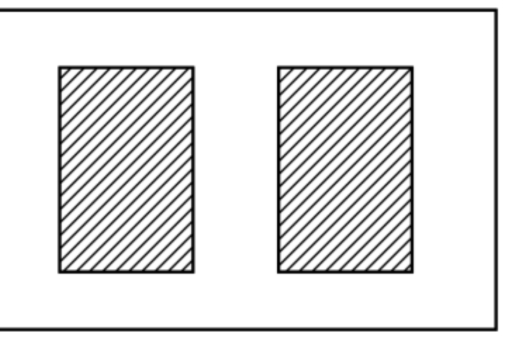
\includegraphics[width=0.34\textwidth]{figures/gao76_q20_poster.png}
\end{center}

\ifanswer
\solbegin
\stepm{(1)}{当 $x>0$ 时，$x+\dfrac1x\geqslant2\sqrt{x\times\dfrac1x}=2$，当且仅当 $x=\dfrac1x$，即 $x=1$ 取等号，}
\step{当 $x<0$ 时，$-x-\dfrac1x\geqslant2\sqrt{(-x)\times\dfrac1{-x}}=2$，所以 $x+\dfrac1x\leqslant-2$，}
\step{当且仅当 $-x=-\dfrac1x$，即 $x=-1$ 取等号，}
\step{综上所述，$x+\dfrac1x$ 的取值范围为 $(-\infty,-2]\cup[2,+\infty)$.}
\stepm{(2)}{设矩形栏目宽为 $x$，高为 $y$，则 $2xy=18000$，}
\step{所以 $S=(2x+36)(y+20)=2xy+36y+40x+720$}
% 原卷此行把 18720 写作 36720，照录（见文件头“原卷笔误/存疑”①）
\step{$=18000+36y+40x+720\geqslant18720+2\sqrt{36y\times40x}$}
\step{$=36720+2\sqrt{36\times40\times18000}=18720+7200=25920$，}
\step{当且仅当 $36y=40x$，即 $x=90$，$y=100$ 取等号，}
\step{所以海报的高为 $120\,\mathrm{cm}$ 与宽为 $216\,\mathrm{cm}$，可使矩形海报面积 $S$ 最小，}
\step{最小面积为 $25920$.}
\solend
\fi

\ansspace

\item 若实数 $x$、$y$、$m$ 满足 $|x-m|>|y-m|$，则称 $x$ 比 $y$ 远离 $m$.

（1）$0$ 比 $\dfrac12$ 远离 $2$ 吗？说明理由；

（2）若 $\dfrac1{2x-1}$ 比 $\dfrac12$ 远离 $1$，求实数 $x$ 的取值范围；

（3）若 $m\leqslant1$，$x+y=2$，试问：$x$ 与 $x^2+y^2$ 哪一个更远离 $m$，并说明理由.

\ifanswer
\solbegin
\stepm{(1)}{$0$ 比 $\dfrac12$ 远离 $2$，理由为：}
\step{由于 $|0-2|=2>\dfrac32=\left|\dfrac12-2\right|$，所以 $0$ 比 $\dfrac12$ 远离 $2$.}
\stepm{(2)}{由 $\dfrac1{2x-1}$ 比 $\dfrac12$ 远离 $1$，得 $\left|\dfrac1{2x-1}-1\right|>\left|\dfrac12-1\right|$，即 $\left|\dfrac1{2x-1}-1\right|>\dfrac12$，}
\step{则 $\dfrac1{2x-1}-1>\dfrac12$ 或 $\dfrac1{2x-1}-1<-\dfrac12$，整理得 $\dfrac1{2x-1}>\dfrac32$ 或 $\dfrac1{2x-1}<\dfrac12$，}
\step{因此 $0<2x-1<\dfrac23$ 或 $2x-1<0$ 或 $2x-1>2$，}
\step{解得 $\dfrac12<x<\dfrac56$ 或 $x<\dfrac12$ 或 $x>\dfrac32$，}
\step{所以 $x$ 的取值范围是 $\left(-\infty,\dfrac12\right)\cup\left(\dfrac12,\dfrac56\right)\cup\left(\dfrac32,+\infty\right)$.}
\stepm{(3)}{$x^2+y^2$ 比 $x$ 更远离 $m$，理由为：}
\step{由 $x^2+y^2\geqslant\dfrac{(x+y)^2}2=2\geqslant m$，得 $|x^2+y^2-m|=x^2+y^2-m$，}
\step{由 $x+y=2$，得 $x^2+y^2=x^2+(2-x)^2=2x^2-4x+4$，}
\step{于是 $|x^2+y^2-m|-|x-m|=2x^2-4x+4-m-|x-m|$，}
\step{当 $x\geqslant m$ 时，$|x^2+y^2-m|-|x-m|=2x^2-4x+4-m-(x-m)$}
\step{$=2\left(x-\dfrac54\right)^2+\dfrac78>0$，即 $|x^2+y^2-m|>|x-m|$；}
\step{当 $x<m$ 时，$|x^2+y^2-m|-|x-m|=2x^2-4x+4-m+(x-m)$}
\step{$=2\left(x-\dfrac34\right)^2+\dfrac{23}8-2m$，}
\step{由 $m\leqslant1$，得 $\dfrac{23}8-2m>0$，因此 $2\left(x-\dfrac34\right)^2+\dfrac{23}8-2m>0$，}
\step{即 $|x^2+y^2-m|>|x-m|$，}
\step{所以 $|x^2+y^2-m|>|x-m|$，即 $x^2+y^2$ 比 $x$ 更远离 $m$.}
\solend
\fi

\ansspace*[7]

\end{enumerate}

\end{document}
"
% 紧凑版：xelatex "\def\iscompact{1}% 高一76_六十中学_10月月考.tex
%   —— 高一上数学“2026-2027 年六十中学高一上 10 月月考”（讲评版）
% 试卷版：xelatex 高一76_六十中学_10月月考.tex
% 答案版：xelatex "\def\isanswer{1}% 高一76_六十中学_10月月考.tex
%   —— 高一上数学“2026-2027 年六十中学高一上 10 月月考”（讲评版）
% 试卷版：xelatex 高一76_六十中学_10月月考.tex
% 答案版：xelatex "\def\isanswer{1}\input{高一76_六十中学_10月月考.tex}"
% 紧凑版：xelatex "\def\iscompact{1}\input{高一76_六十中学_10月月考.tex}"
%
% 原始材料：微信公众号“魔都数学加油站”文章，连载“27学年高一76”；
% 原文标题“27学年高一76——2026-2027年上海市六十中学高一上10月月考”；
% 原文链接：https://mp.weixin.qq.com/s/GrKZjQrV1Xb0wy0BUuzAHw。
% 页面标注发布时间 2026-10-22 21:45（上海）。
% 正文为 10 张 PNG 页（`原图/高一76_六十中学_10月月考/01..10.png`）：
% 第 4、5、8、9 页为 4762×6735，其余 6 页为 2560×3620，均按页序读取。
% 10 页全为试卷正文页（卷首标题在第 1 页页顶，卷末第 21 题 (3) 解析止于第 10 页），
% 无封面页、目录页、二维码或宣传页。粉色斜排“魔都数学加油站”为卷面水印，未录入。
%
% 卷首标题：照卷面印作“2026-2027 年六十中学高一上 10 月月考”（黑体加粗一行）。
% 原卷年份区间用半角连字符，本稿按全稿惯例排 en dash；原卷无副标题。
%
% 篇幅与题号：原卷自第 3 题起编号（第 1、2 题不在本卷内）。填空题 3—12（10 题）、
% 选择题 13—16（4 题）、解答题 17—21（5 题），共 19 题。本稿沿用原节与原题号，
% 只改排为全稿统一的大节样式。
%
% 讲评版：原卷第 3、5 题只印【答案】（“$(0,1)$”“$a$、$b$ 都不能被 $3$ 整除”），
% 本稿只给 \ans{}；其余 17 题均印【解析】，用 \solbegin…\solend。四道选择题的作答
% 括号原卷即留空，答案写在解析末句“故选 C／B／C／D”，照录在解析内，不另提 \ans{}。
%
% 副标题：原卷未印副标题。本稿按“知识模块”口径标作“集合与常用逻辑用语、不等式”：
% 19 题中集合与常用逻辑用语 6 题（第 5、12、14、16、19 题及第 4 题的恒等变形），
% 不等式 13 题（第 3、6—11、13、15、17、18、20、21 题），两类均确有分量，故并标。
% 口径同 高一63、高一68—75。
%
% 与原卷的排版差异：
%   ① 原卷每题下直接印【答案】/【解析】，本稿按全稿惯例将答案与解析置于答案版；
%   ② 原卷未印副标题，本稿按“知识模块”口径补出；
%   ③ 原卷填空横线约四个字宽，本稿按全稿惯例统一排 \blankline[4.4em]；
%   ④ 原卷数集记号排斜体 $R$、$N$（第 4、6、7、8、11、12、14、15、19、20 题），本稿
%      按全稿惯例改用 $\R$、$\N$（同 高一68—75）；第 7、19、20 题的“解集为 $\R$”同此；
%   ⑤ 原卷句末标点多为西文句点，均逐处照录；
%   ⑥ 第 17—21 题的子问原卷印作“（1）…（2）…”，本稿按 高一69—75 成例用行内
%      “（1）（2）（3）”段，解析中的子问标号用 \stepm{(1)}{…}；
%   ⑦ 每道解答题原卷未留作答空白，本稿按全稿惯例加 \ansspace（末题用 \ansspace*）；
%   ⑧ 选择题的作答括号原卷排半角“(    )”，本稿按全稿惯例排 \mbox{（\quad）}；
%      选项行排照原卷——第 13、14、15、16 题一行两条、分两行排（本稿按原卷分行）；
%   ⑨ 第 10、11、17—21 题解析中的不等式组／方程组，原卷均排作“{”连接的多行式，
%      本稿按全稿惯例排 cases；
%   ⑩ 第 14 题题干右侧有一幅韦恩图（全集矩形内含 A、B 两圆，B 涂灰）：本稿按原卷
%      截图裁取（`figures/gao76_q14_venn.png`，由第 5 页原图裁出、去除粉色水印后转
%      灰度，未放大），放在题干之后、选项之前，仅答案版出；
%   ⑪ 第 20 题 (2) 题干右侧有一幅示意图（大矩形内两个斜线阴影小矩形）：本稿按原卷
%      截图裁取（`figures/gao76_q20_poster.png`，由第 8 页原图裁出、去除粉色水印后转
%      灰度，未放大），放在该小题文字之后，仅答案版出。
%
% 原卷笔误/存疑（均照录未改，正文对应处另有 % 注）：
%   ① 第 20 题 (2) 解析第 3 行把 $2xy+720$ 写成 $36720$（实为 $18000+720=18720$），
%      同式下一行又写回 $18720$，前后不一致；原卷如此，照录未改。
%   ② 第 14 题的韦恩图阴影是把整个 $B$ 圆（含 $A\cap B$ 部分）涂灰，而解析按
%      $\overline{A\cap B}$ 求解，二者不一致；原卷图文如此，照录未改。
%
% 行数核对：逐题数 \step/\stepm 条数与原卷【解析】印刷行数，17 题逐一相符，
% 合计 118 条 / 118 行（Q4：3；Q6：4；Q7：1；Q8：6；Q9：3；Q10：7；Q11：4；
% Q12：16；Q13：1；Q14：3；Q15：7；Q16：10；Q17：12；Q18：6；Q19：6；Q20：11；
% Q21：18）。另第 3、5 题只印【答案】，各提 \ans{}，不计入 \step 账。
%
% 插图：第 14 题题干的韦恩图、第 20 题 (2) 的示意图，见上⑩⑪；其余题干无配图。
%
\documentclass[a4paper,11pt]{article}
\usepackage{common}

\begin{document}

\examtitlest[3]{2026--2027 年六十中学高一上 10 月月考}{集合与常用逻辑用语、不等式}

\bigsec{一、填空题}

\begin{enumerate}
\setcounter{enumi}{2}

\item 不等式 $\dfrac{x}{1-x}>0$ 的解集是\blankline[4.4em].

\ifanswer
\ans{$(0,1)$}
\fi

\item 已知 $2x^2+x+1=a(x+1)^2+b(x+1)+2$，对 $x\in\R$ 恒成立，$ab=$\blankline[4.4em].

\ifanswer
\solbegin
\step{若 $2x^2+x+1=a(x+1)^2+b(x+1)+2$ 对 $x\in\R$ 恒成立，}
\step{即 $2x^2+x+1=ax^2+(2a+b)x+a+b+2$ 对 $x\in\R$ 恒成立，}
\step{必有 $\begin{cases}a=2\\ 2a+b=1\\ a+b+2=1\end{cases}$，解得 $a=2$，$b=-3$，所以 $ab=-6$.}
\solend
\fi

\item 利用反证法证明命题：“如果 $a$、$b\in\N$，$ab$ 可被 $3$ 整除，那么 $a$、$b$ 中至少有一个能被 $3$ 整除”时，假设的内容应是\blankline[4.4em].

\ifanswer
\ans{$a$、$b$ 都不能被 $3$ 整除}
\fi

\item 已知 $x\in\R$，方程 $|x+1|+|2-x|=3$ 的解集为\blankline[4.4em].

\ifanswer
\solbegin
\step{当 $x<-1$ 时，则 $|x+1|+|2-x|=-x-1+2-x=1-2x>3$；}
\step{当 $-1\leqslant x\leqslant2$ 时，则 $|x+1|+|2-x|=x+1+2-x=3$；}
\step{当 $x>2$ 时，则 $|x+1|+|2-x|=x+1+x-2=2x-1>3$.}
\step{综上所述，原方程的解集为 $[-1,2]$.}
\solend
\fi

\item 若关于 $x$ 的不等式 $x^2+kx+1\geqslant0$ 的解集为 $\R$，则实数 $k$ 的取值范围是\blankline[4.4em].

\ifanswer
\solbegin
\step{$\Delta=k^2-4\leqslant0\Rightarrow-2\leqslant k\leqslant2$，所以实数 $k$ 的取值范围是 $[-2,2]$.}
\solend
\fi

\item 已知 $a$、$b\in\R$，且 $ab>0$，则下列不等式中，恒成立的序号是\blankline[4.4em].

① $a^2+b^2>2ab$；② $a+b\geqslant2\sqrt{ab}$；③ $\dfrac1a+\dfrac1b>\dfrac2{\sqrt{ab}}$；④ $\dfrac ba+\dfrac ab\geqslant2$.

\ifanswer
\solbegin
\step{因为 $a^2+b^2\geqslant2ab$ 对于 $a$、$b\in\R$ 恒成立，当且仅当 $a=b$ 时取等号，}
\step{所以①错误；}
\step{对于②，③，显然 $a<0$，$b<0$ 时，不等式均不成立，即②和③错误；}
\step{对于④，因为 $ab>0$，所以 $\dfrac ba>0,\dfrac ab>0$，}
\step{由基本不等式得 $\dfrac ba+\dfrac ab\geqslant2\sqrt{\dfrac ba\cdot\dfrac ab}=2$，即④正确.}
\step{故正确的是④.}
\solend
\fi

\item 已知正实数 $m$、$n$ 满足 $m+\dfrac2n=1$，则 $\dfrac1m+2n$ 的最小值为\blankline[4.4em].

\ifanswer
\solbegin
\step{$\dfrac1m+2n=\left(m+\dfrac2n\right)\left(\dfrac1m+2n\right)=5+2mn+\dfrac2{mn}$，}
\step{因为 $mn>0$，所以 $2mn+\dfrac2{mn}\geqslant2\sqrt{2mn\cdot\dfrac2{mn}}=4$，}
\step{当且仅当 $2mn=\dfrac2{mn}$，即 $m=\dfrac13$，$n=3$ 时取等号，所以 $\dfrac1m+2n$ 的最小值为 $9$.}
\solend
\fi

\item 若关于 $x$ 的不等式组 $\begin{cases}3x+1>0\\ x+\dfrac1a\leqslant2\end{cases}$ 恰好有两个整数解，则实数 $a$ 的取值范围为\blankline[4.4em].

\ifanswer
\solbegin
\step{由 $3x+1>0$ 得 $x>-\dfrac13$；若 $a<0$，则 $\dfrac1a<0$，由 $x+\dfrac1a\leqslant2$ 得 $x\leqslant2-\dfrac1a>2$，}
\step{则解集 $\left(-\dfrac13,2-\dfrac1a\right]$ 必同时含有整数 $0$、$1$、$2$，不合题意；}
\step{又 $a=0$ 使 $\dfrac1a$ 无意义，故 $a>0$；}
\step{此时原不等式组的解集为 $\left(-\dfrac13,2-\dfrac1a\right]$，}
\step{其中大于 $-\dfrac13$ 的整数依次为 $0$，$1$，$2$，$\cdots$，}
\step{恰有两个整数解即解集只含 $0$ 与 $1$，故 $1\leqslant2-\dfrac1a<2$，即 $\dfrac1a\leqslant1$ 且 $\dfrac1a>0$，}
\step{结合 $a>0$，解得 $a\geqslant1$.}
\solend
\fi

\item 已知 $a\in\R$，若关于 $x$ 的方程 $x^2+ax+a^2-8=0$ 有两个实根 $x_1$、$x_2$，且 $\dfrac1{x_1}+\dfrac1{x_2}=-\dfrac12$，则 $a$ 的值为\blankline[4.4em].

\ifanswer
\solbegin
\step{由题意得 $\Delta=a^2-4(a^2-8)=32-3a^2\geqslant0$，解得 $a^2\leqslant\dfrac{32}3$，}
\step{由韦达定理得 $x_1+x_2=-a$，$x_1x_2=a^2-8$，}
\step{则 $\dfrac1{x_1}+\dfrac1{x_2}=\dfrac{x_1+x_2}{x_1x_2}=\dfrac{-a}{a^2-8}=-\dfrac12$，即 $a^2-2a-8=(a-4)(a+2)=0$，}
\step{解得 $a=4$ 或 $a=-2$，又 $a^2\leqslant\dfrac{32}3$，则 $a=-2$.}
\solend
\fi

\item 已知有限集 $A=\{a_1,a_2,\cdots,a_n\}(n\geqslant2,n\in\N)$，若 $A$ 中元素 $a_i(i=1,2,\cdots,n)$ 满足 $a_1+a_2+\cdots+a_n=a_1\times a_2\times\cdots\times a_n$，就称 $A$ 为“完美集”，以下四个命题：

①集合 $\{-1-\sqrt3,-1+\sqrt3\}$ 不是“完美集”；

②若 $a_1$、$a_2$ 是两个不同的正数，且 $\{a_1,a_2\}$ 是“完美集”，则 $a_1$、$a_2$ 至少有一个大于 $2$；

③二元“完美集”有无穷多个；

④若 $a_i$ 均为正整数，则“完美集”$A$ 有且只有一个，且 $n=3$.

其中，真命题的序号是\blankline[4.4em].

\ifanswer
\solbegin
\step{对于①选项：$(-1-\sqrt3)+(-1+\sqrt3)=-2$，$(-1-\sqrt3)\times(-1+\sqrt3)=-2$，}
\step{故 $(-1-\sqrt3)+(-1+\sqrt3)=(-1-\sqrt3)\times(-1+\sqrt3)$，}
\step{所以集合 $\{-1-\sqrt3,-1+\sqrt3\}$ 是“完美集”，故①错误；}
\step{对于②选项：集合 $\{a_1,a_2\}$ 是“完美集”，设 $a_1+a_2=a_1a_2=t>0$，}
\step{则 $a_1$、$a_2$ 可以看成一元二次方程 $x^2-tx+t=0$ 的两正根，则 $\Delta=t^2-4t>0$，}
\step{解得 $t<0$（舍）或 $t>4$，即 $a_1a_2>4$，所以至少有一个大于 $2$，故②正确；}
\step{对于③选项：由②得一元二次方程 $x^2-tx+t=0$ 当 $t$ 取不同值时，}
\step{$a_1$、$a_2$ 的值是不同的，因而二元“完美集”有无穷多个，故③正确；}
\step{对于④选项：设 $a_1<a_2<a_3<\cdots<a_n$，}
\step{则 $a_1\times a_2\times\cdots\times a_n=a_1+a_2+\cdots+a_n<na_n$，}
\step{所以 $a_1\times a_2\times\cdots\times a_{n-1}<n$，又 $a_i\in\N^*$，所以 $n\leqslant3$，}
\step{当 $n=2$ 时，$a_1<2$，则 $a_1=1$，$a_1a_2\neq a_1+a_2$，不合题意，}
\step{当 $n=3$ 时，$a_1a_2<3$，所以只能是 $a_1=1$，$a_2=2$，}
\step{由 $a_1+a_2+a_3=a_1a_2a_3$，代入解得 $a_3=3$，所以此时“完美集”只有一个，}
\step{为 $\{1,2,3\}$，故④正确.}
\step{故正确的是②③④.}
\solend
\fi

\end{enumerate}

\bigsec{二、选择题}

\begin{enumerate}
\setcounter{enumi}{12}

\item 已知 $x$、$y\in\R$，则“$xy\geqslant0$”是“$xy=|xy|$”的\mbox{（\quad）}

\keepwithprev
A. 充分非必要条件\qquad B. 必要非充分条件

C. 充要条件\qquad D. 既非充分也非必要条件

\ifanswer
\solbegin
\step{$xy\geqslant0\Leftrightarrow xy=|xy|$，故“$xy\geqslant0$”是“$xy=|xy|$”的充要条件. 故选 $C$.}
\solend
\fi

\needvspace{22\baselineskip}
\item 已知全集 $U=\R$，集合 $A=\{x\mid x<-1\text{ 或 }x>4\}$，$B=\{x\mid x^2-x-6\leqslant0\}$，则阴影部分表示的集合为\mbox{（\quad）}

\begin{center}
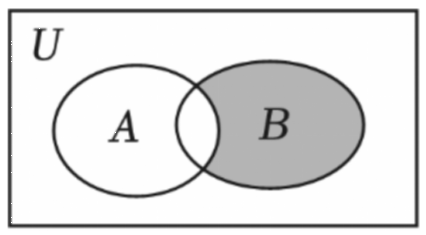
\includegraphics[width=0.26\textwidth]{figures/gao76_q14_venn.png}
\end{center}

\keepwithprev
A. $\{x\mid-2\leqslant x<4\}$\qquad B. $\{x\mid-1\leqslant x\leqslant3\}$

C. $\{x\mid x\leqslant3\text{ 或 }x\geqslant4\}$\qquad D. $\{x\mid-2\leqslant x\leqslant4\}$

\ifanswer
\solbegin
\step{全集 $U=\R$，集合 $A=\{x\mid x<-1\text{ 或 }x>4\}$，}
\step{$B=\{x\mid x^2-x-6\leqslant0\}=\{x\mid-2\leqslant x\leqslant3\}$，故 $A\cap B=\{x\mid-2\leqslant x<-1\}$，}
\step{故阴影部分表示的集合为 $\overline{A\cap B}=\{x\mid-1\leqslant x\leqslant3\}$. 故选 $B$.}
\solend
\fi

\item 设 $a$、$b$、$c\in\R$，给出下列命题：①若 $a>b$，则 $a^2>b^2$，②“$a>b$”是“$a^3>b^3$”的充要条件，③若 $a^2>b^2$，则 $|a|>|b|$，④若 $\dfrac ab>1$，则 $a>b$，⑤若 $a>b$，$c\neq0$，则 $\dfrac a{c^2}>\dfrac b{c^2}$，其中真命题的个数是\mbox{（\quad）}

\keepwithprev
A. $1$ 个\qquad B. $2$ 个\qquad C. $3$ 个\qquad D. $4$ 个

\ifanswer
\solbegin
\step{对于①，取 $a=2$，$b=-2$，满足 $a>b$，而 $a^2=b^2$，故为假命题；}
\step{对于②，$a>b\Leftrightarrow a^3-b^3=(a-b)(a^2+ab+b^2)=(a-b)\left[\left(a+\dfrac12b\right)^2+\dfrac34b^2\right]>0$}
\step{$\Leftrightarrow a^3>b^3$，故为真命题；}
\step{对于③，$a^2>b^2\Leftrightarrow|a|^2>|b|^2\Leftrightarrow|a|>|b|$，故为真命题；}
\step{对于④，取 $a=-2$，$b=-1$，满足 $\dfrac ab>1$，而 $a<b$，故为假命题；}
\step{对于⑤，由题意得 $c^2>0$，由 $a>b$，则 $\dfrac a{c^2}>\dfrac b{c^2}$，故为真命题.}
\step{故选 $C$.}
\solend
\fi

\item 已知关于 $x$ 的两个一元二次不等式 $a_1x^2+b_1x+c_1>0$，$a_2x^2+b_2x+c_2>0$ 的解集分别为 $A$、$B$，其中 $a_i$、$b_i$、$c_i(i=1,2)$ 为常数且不为零，则“$\dfrac{a_1}{a_2}=\dfrac{b_1}{b_2}=\dfrac{c_1}{c_2}$”是“$A=B$”\mbox{（\quad）}

\keepwithprev
A. 充分不必要条件\qquad B. 必要不充分条件

C. 充要条件\qquad D. 既不充分也不必要条件

\ifanswer
\solbegin
\step{设 $\dfrac{a_1}{a_2}=\dfrac{b_1}{b_2}=\dfrac{c_1}{c_2}=\lambda$，}
\step{①当 $\lambda>0$ 时，则 $a_1=\lambda a_2$，$b_1=\lambda b_2$，$c_1=\lambda c_2$，}
\step{$a_1x^2+b_1x+c_1>0\Leftrightarrow\lambda a_2x^2+\lambda b_2x+\lambda c_2>0\Leftrightarrow a_2x^2+b_2x+c_2>0$，}
\step{所以 $A=B$，}
\step{②当 $\lambda<0$ 时，则 $a_1=\lambda a_2$，$b_1=\lambda b_2$，$c_1=\lambda c_2$，}
\step{$a_1x^2+b_1x+c_1>0\Leftrightarrow\lambda a_2x^2+\lambda b_2x+\lambda c_2>0\Leftrightarrow a_2x^2+b_2x+c_2<0$，}
\step{所以 $A\neq B$，充分性不成立，}
\step{当 $A=B=\R$ 时，则 $\Delta<0$ 且 $a_1$、$a_2>0$，$\dfrac{a_1}{a_2}=\dfrac{b_1}{b_2}=\dfrac{c_1}{c_2}$ 不一定成立，}
\step{必要性不成立.}
\step{所以 $\dfrac{a_1}{a_2}=\dfrac{b_1}{b_2}=\dfrac{c_1}{c_2}$ 是 $A=B$ 的既不充分也不必要条件，故选 $D$.}
\solend
\fi

\end{enumerate}

\bigsec{三、解答题}

\begin{enumerate}
\setcounter{enumi}{16}

\item 求下列关于 $x$ 的不等式（组）的解集.

（1）$\begin{cases}9x^2-6x-24>0\\ \dfrac{x+3}{x-1}>2\end{cases}$；

（2）$|2x+1|-|2-x|>2$.

\ifanswer
\solbegin
\stepm{(1)}{不等式 $\dfrac{x+3}{x-1}>2$ 可化为 $\dfrac{x+3}{x-1}-2>0$，}
\step{即 $\dfrac{-x+5}{x-1}>0$，即 $(x-1)(x-5)<0$，解得 $1<x<5$，}
\step{不等式 $9x^2-6x-24>0$ 可化为 $(3x+4)(x-2)>0$，}
\step{解得 $x<-\dfrac43$ 或 $x>2$，}
\step{所以不等式的解集为 $(2,5)$.}
\stepm{(2)}{当 $x\leqslant-\dfrac12$ 时，$|2x+1|-|2-x|>2$ 等价于 $-2x-1-(2-x)>2$，}
\step{解得 $x<-5$，所以 $x<-5$，}
\step{当 $-\dfrac12<x<2$ 时，$|2x+1|-|2-x|>2$ 等价于 $2x+1-(2-x)>2$，}
\step{解得 $x>1$，所以 $1<x<2$，}
\step{当 $x\geqslant2$ 时，$|2x+1|-|2-x|>2$ 等价于 $2x+1-(x-2)>2$，}
\step{解得 $x>-1$，所以 $x\geqslant2$，}
\step{综上，$|2x+1|-|2-x|>2$ 的解集为 $(-\infty,-5)\cup(1,+\infty)$.}
\solend
\fi

\ansspace

\item 设 $m$ 为实数，求关于 $x$ 与 $y$ 的二元一次方程组 $\begin{cases}y=x+m\\ mx-y=4\end{cases}$ 的解集.

\ifanswer
\solbegin
\step{消去 $y$ 得 $(m-1)x=m+4$，}
\step{当 $m-1=0$，即 $m=1$ 时，$0=5$ 不成立，则 $x$ 无解，原方程组的解集为 $\varnothing$；}
\step{当 $m-1\neq0$，即 $m\neq1$ 时，则 $x=\dfrac{m+4}{m-1}$，$y=\dfrac{m+4}{m-1}+m=\dfrac{m^2+4}{m-1}$，}
\step{原方程组的解集为 $\left\{\left(\dfrac{m+4}{m-1},\dfrac{m^2+4}{m-1}\right)\right\}$.}
\step{综上所述，当 $m=1$ 时，方程组的解集为 $\varnothing$；}
\step{当 $m\neq1$ 时，方程组的解集为 $\left\{\left(\dfrac{m+4}{m-1},\dfrac{m^2+4}{m-1}\right)\right\}$.}
\solend
\fi

\ansspace

\item 已知集合 $A=\{x\mid-2\leqslant x-1\leqslant5\}$，集合 $B=\{x\mid m+1\leqslant x\leqslant2m-1\}(m\in\R)$.

（1）若 $m=4$，全集 $U=\R$，求 $A\cap B$；

（2）设命题 $p:x\in A$；命题 $q:x\in B$，若命题 $p$ 是命题 $q$ 的必要不充分条件，求实数 $m$ 的取值范围.

\ifanswer
\solbegin
\stepm{(1)}{由题意得 $A=\{x\mid-2\leqslant x-1\leqslant5\}=\{x\mid-1\leqslant x\leqslant6\}$，}
\step{当 $m=4$ 时，$B=\{x\mid5\leqslant x\leqslant7\}$，$A\cap B=\{x\mid5\leqslant x\leqslant6\}$；}
\stepm{(2)}{因为命题 $p$ 是命题 $q$ 的必要不充分条件，所以集合 $B$ 是集合 $A$ 的真子集，}
\step{当 $B=\varnothing$ 时，$m+1>2m-1$，解得 $m<2$，}
\step{当 $B\neq\varnothing$ 时，$\begin{cases}m+1\leqslant2m-1\\ m+1\geqslant-1\\ 2m-1\leqslant6\end{cases}$（等号不能同时成立），解得 $2\leqslant m\leqslant\dfrac72$，}
\step{综上所述，实数 $m$ 的取值范围为 $\left(-\infty,\dfrac72\right]$.}
\solend
\fi

\ansspace

\item （1）已知实数 $x\neq0$，求 $x+\dfrac1x$ 的取值范围；

（2）如图，要设计一张矩形海报，该海报含有大小相等的左右两个矩形栏目（即图中阴影部分），这两栏的面积之和为 $18000\,\mathrm{cm}^2$，四周空白的宽度为 $10\,\mathrm{cm}$，两栏之间的中缝空白的宽度为 $16\,\mathrm{cm}$，怎样确定海报的高与宽的尺寸（单位：$\mathrm{cm}$），能使矩形海报面积 $S$ 最小？最小面积是多少？

\begin{center}
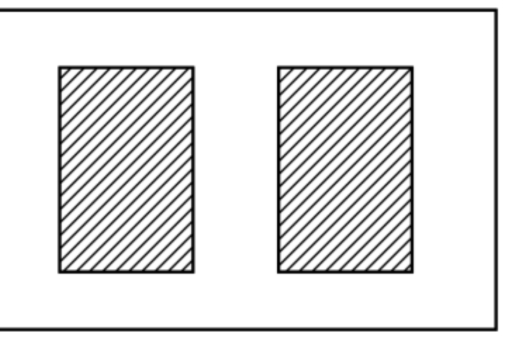
\includegraphics[width=0.34\textwidth]{figures/gao76_q20_poster.png}
\end{center}

\ifanswer
\solbegin
\stepm{(1)}{当 $x>0$ 时，$x+\dfrac1x\geqslant2\sqrt{x\times\dfrac1x}=2$，当且仅当 $x=\dfrac1x$，即 $x=1$ 取等号，}
\step{当 $x<0$ 时，$-x-\dfrac1x\geqslant2\sqrt{(-x)\times\dfrac1{-x}}=2$，所以 $x+\dfrac1x\leqslant-2$，}
\step{当且仅当 $-x=-\dfrac1x$，即 $x=-1$ 取等号，}
\step{综上所述，$x+\dfrac1x$ 的取值范围为 $(-\infty,-2]\cup[2,+\infty)$.}
\stepm{(2)}{设矩形栏目宽为 $x$，高为 $y$，则 $2xy=18000$，}
\step{所以 $S=(2x+36)(y+20)=2xy+36y+40x+720$}
% 原卷此行把 18720 写作 36720，照录（见文件头“原卷笔误/存疑”①）
\step{$=18000+36y+40x+720\geqslant18720+2\sqrt{36y\times40x}$}
\step{$=36720+2\sqrt{36\times40\times18000}=18720+7200=25920$，}
\step{当且仅当 $36y=40x$，即 $x=90$，$y=100$ 取等号，}
\step{所以海报的高为 $120\,\mathrm{cm}$ 与宽为 $216\,\mathrm{cm}$，可使矩形海报面积 $S$ 最小，}
\step{最小面积为 $25920$.}
\solend
\fi

\ansspace

\item 若实数 $x$、$y$、$m$ 满足 $|x-m|>|y-m|$，则称 $x$ 比 $y$ 远离 $m$.

（1）$0$ 比 $\dfrac12$ 远离 $2$ 吗？说明理由；

（2）若 $\dfrac1{2x-1}$ 比 $\dfrac12$ 远离 $1$，求实数 $x$ 的取值范围；

（3）若 $m\leqslant1$，$x+y=2$，试问：$x$ 与 $x^2+y^2$ 哪一个更远离 $m$，并说明理由.

\ifanswer
\solbegin
\stepm{(1)}{$0$ 比 $\dfrac12$ 远离 $2$，理由为：}
\step{由于 $|0-2|=2>\dfrac32=\left|\dfrac12-2\right|$，所以 $0$ 比 $\dfrac12$ 远离 $2$.}
\stepm{(2)}{由 $\dfrac1{2x-1}$ 比 $\dfrac12$ 远离 $1$，得 $\left|\dfrac1{2x-1}-1\right|>\left|\dfrac12-1\right|$，即 $\left|\dfrac1{2x-1}-1\right|>\dfrac12$，}
\step{则 $\dfrac1{2x-1}-1>\dfrac12$ 或 $\dfrac1{2x-1}-1<-\dfrac12$，整理得 $\dfrac1{2x-1}>\dfrac32$ 或 $\dfrac1{2x-1}<\dfrac12$，}
\step{因此 $0<2x-1<\dfrac23$ 或 $2x-1<0$ 或 $2x-1>2$，}
\step{解得 $\dfrac12<x<\dfrac56$ 或 $x<\dfrac12$ 或 $x>\dfrac32$，}
\step{所以 $x$ 的取值范围是 $\left(-\infty,\dfrac12\right)\cup\left(\dfrac12,\dfrac56\right)\cup\left(\dfrac32,+\infty\right)$.}
\stepm{(3)}{$x^2+y^2$ 比 $x$ 更远离 $m$，理由为：}
\step{由 $x^2+y^2\geqslant\dfrac{(x+y)^2}2=2\geqslant m$，得 $|x^2+y^2-m|=x^2+y^2-m$，}
\step{由 $x+y=2$，得 $x^2+y^2=x^2+(2-x)^2=2x^2-4x+4$，}
\step{于是 $|x^2+y^2-m|-|x-m|=2x^2-4x+4-m-|x-m|$，}
\step{当 $x\geqslant m$ 时，$|x^2+y^2-m|-|x-m|=2x^2-4x+4-m-(x-m)$}
\step{$=2\left(x-\dfrac54\right)^2+\dfrac78>0$，即 $|x^2+y^2-m|>|x-m|$；}
\step{当 $x<m$ 时，$|x^2+y^2-m|-|x-m|=2x^2-4x+4-m+(x-m)$}
\step{$=2\left(x-\dfrac34\right)^2+\dfrac{23}8-2m$，}
\step{由 $m\leqslant1$，得 $\dfrac{23}8-2m>0$，因此 $2\left(x-\dfrac34\right)^2+\dfrac{23}8-2m>0$，}
\step{即 $|x^2+y^2-m|>|x-m|$，}
\step{所以 $|x^2+y^2-m|>|x-m|$，即 $x^2+y^2$ 比 $x$ 更远离 $m$.}
\solend
\fi

\ansspace*[7]

\end{enumerate}

\end{document}
"
% 紧凑版：xelatex "\def\iscompact{1}% 高一76_六十中学_10月月考.tex
%   —— 高一上数学“2026-2027 年六十中学高一上 10 月月考”（讲评版）
% 试卷版：xelatex 高一76_六十中学_10月月考.tex
% 答案版：xelatex "\def\isanswer{1}\input{高一76_六十中学_10月月考.tex}"
% 紧凑版：xelatex "\def\iscompact{1}\input{高一76_六十中学_10月月考.tex}"
%
% 原始材料：微信公众号“魔都数学加油站”文章，连载“27学年高一76”；
% 原文标题“27学年高一76——2026-2027年上海市六十中学高一上10月月考”；
% 原文链接：https://mp.weixin.qq.com/s/GrKZjQrV1Xb0wy0BUuzAHw。
% 页面标注发布时间 2026-10-22 21:45（上海）。
% 正文为 10 张 PNG 页（`原图/高一76_六十中学_10月月考/01..10.png`）：
% 第 4、5、8、9 页为 4762×6735，其余 6 页为 2560×3620，均按页序读取。
% 10 页全为试卷正文页（卷首标题在第 1 页页顶，卷末第 21 题 (3) 解析止于第 10 页），
% 无封面页、目录页、二维码或宣传页。粉色斜排“魔都数学加油站”为卷面水印，未录入。
%
% 卷首标题：照卷面印作“2026-2027 年六十中学高一上 10 月月考”（黑体加粗一行）。
% 原卷年份区间用半角连字符，本稿按全稿惯例排 en dash；原卷无副标题。
%
% 篇幅与题号：原卷自第 3 题起编号（第 1、2 题不在本卷内）。填空题 3—12（10 题）、
% 选择题 13—16（4 题）、解答题 17—21（5 题），共 19 题。本稿沿用原节与原题号，
% 只改排为全稿统一的大节样式。
%
% 讲评版：原卷第 3、5 题只印【答案】（“$(0,1)$”“$a$、$b$ 都不能被 $3$ 整除”），
% 本稿只给 \ans{}；其余 17 题均印【解析】，用 \solbegin…\solend。四道选择题的作答
% 括号原卷即留空，答案写在解析末句“故选 C／B／C／D”，照录在解析内，不另提 \ans{}。
%
% 副标题：原卷未印副标题。本稿按“知识模块”口径标作“集合与常用逻辑用语、不等式”：
% 19 题中集合与常用逻辑用语 6 题（第 5、12、14、16、19 题及第 4 题的恒等变形），
% 不等式 13 题（第 3、6—11、13、15、17、18、20、21 题），两类均确有分量，故并标。
% 口径同 高一63、高一68—75。
%
% 与原卷的排版差异：
%   ① 原卷每题下直接印【答案】/【解析】，本稿按全稿惯例将答案与解析置于答案版；
%   ② 原卷未印副标题，本稿按“知识模块”口径补出；
%   ③ 原卷填空横线约四个字宽，本稿按全稿惯例统一排 \blankline[4.4em]；
%   ④ 原卷数集记号排斜体 $R$、$N$（第 4、6、7、8、11、12、14、15、19、20 题），本稿
%      按全稿惯例改用 $\R$、$\N$（同 高一68—75）；第 7、19、20 题的“解集为 $\R$”同此；
%   ⑤ 原卷句末标点多为西文句点，均逐处照录；
%   ⑥ 第 17—21 题的子问原卷印作“（1）…（2）…”，本稿按 高一69—75 成例用行内
%      “（1）（2）（3）”段，解析中的子问标号用 \stepm{(1)}{…}；
%   ⑦ 每道解答题原卷未留作答空白，本稿按全稿惯例加 \ansspace（末题用 \ansspace*）；
%   ⑧ 选择题的作答括号原卷排半角“(    )”，本稿按全稿惯例排 \mbox{（\quad）}；
%      选项行排照原卷——第 13、14、15、16 题一行两条、分两行排（本稿按原卷分行）；
%   ⑨ 第 10、11、17—21 题解析中的不等式组／方程组，原卷均排作“{”连接的多行式，
%      本稿按全稿惯例排 cases；
%   ⑩ 第 14 题题干右侧有一幅韦恩图（全集矩形内含 A、B 两圆，B 涂灰）：本稿按原卷
%      截图裁取（`figures/gao76_q14_venn.png`，由第 5 页原图裁出、去除粉色水印后转
%      灰度，未放大），放在题干之后、选项之前，仅答案版出；
%   ⑪ 第 20 题 (2) 题干右侧有一幅示意图（大矩形内两个斜线阴影小矩形）：本稿按原卷
%      截图裁取（`figures/gao76_q20_poster.png`，由第 8 页原图裁出、去除粉色水印后转
%      灰度，未放大），放在该小题文字之后，仅答案版出。
%
% 原卷笔误/存疑（均照录未改，正文对应处另有 % 注）：
%   ① 第 20 题 (2) 解析第 3 行把 $2xy+720$ 写成 $36720$（实为 $18000+720=18720$），
%      同式下一行又写回 $18720$，前后不一致；原卷如此，照录未改。
%   ② 第 14 题的韦恩图阴影是把整个 $B$ 圆（含 $A\cap B$ 部分）涂灰，而解析按
%      $\overline{A\cap B}$ 求解，二者不一致；原卷图文如此，照录未改。
%
% 行数核对：逐题数 \step/\stepm 条数与原卷【解析】印刷行数，17 题逐一相符，
% 合计 118 条 / 118 行（Q4：3；Q6：4；Q7：1；Q8：6；Q9：3；Q10：7；Q11：4；
% Q12：16；Q13：1；Q14：3；Q15：7；Q16：10；Q17：12；Q18：6；Q19：6；Q20：11；
% Q21：18）。另第 3、5 题只印【答案】，各提 \ans{}，不计入 \step 账。
%
% 插图：第 14 题题干的韦恩图、第 20 题 (2) 的示意图，见上⑩⑪；其余题干无配图。
%
\documentclass[a4paper,11pt]{article}
\usepackage{common}

\begin{document}

\examtitlest[3]{2026--2027 年六十中学高一上 10 月月考}{集合与常用逻辑用语、不等式}

\bigsec{一、填空题}

\begin{enumerate}
\setcounter{enumi}{2}

\item 不等式 $\dfrac{x}{1-x}>0$ 的解集是\blankline[4.4em].

\ifanswer
\ans{$(0,1)$}
\fi

\item 已知 $2x^2+x+1=a(x+1)^2+b(x+1)+2$，对 $x\in\R$ 恒成立，$ab=$\blankline[4.4em].

\ifanswer
\solbegin
\step{若 $2x^2+x+1=a(x+1)^2+b(x+1)+2$ 对 $x\in\R$ 恒成立，}
\step{即 $2x^2+x+1=ax^2+(2a+b)x+a+b+2$ 对 $x\in\R$ 恒成立，}
\step{必有 $\begin{cases}a=2\\ 2a+b=1\\ a+b+2=1\end{cases}$，解得 $a=2$，$b=-3$，所以 $ab=-6$.}
\solend
\fi

\item 利用反证法证明命题：“如果 $a$、$b\in\N$，$ab$ 可被 $3$ 整除，那么 $a$、$b$ 中至少有一个能被 $3$ 整除”时，假设的内容应是\blankline[4.4em].

\ifanswer
\ans{$a$、$b$ 都不能被 $3$ 整除}
\fi

\item 已知 $x\in\R$，方程 $|x+1|+|2-x|=3$ 的解集为\blankline[4.4em].

\ifanswer
\solbegin
\step{当 $x<-1$ 时，则 $|x+1|+|2-x|=-x-1+2-x=1-2x>3$；}
\step{当 $-1\leqslant x\leqslant2$ 时，则 $|x+1|+|2-x|=x+1+2-x=3$；}
\step{当 $x>2$ 时，则 $|x+1|+|2-x|=x+1+x-2=2x-1>3$.}
\step{综上所述，原方程的解集为 $[-1,2]$.}
\solend
\fi

\item 若关于 $x$ 的不等式 $x^2+kx+1\geqslant0$ 的解集为 $\R$，则实数 $k$ 的取值范围是\blankline[4.4em].

\ifanswer
\solbegin
\step{$\Delta=k^2-4\leqslant0\Rightarrow-2\leqslant k\leqslant2$，所以实数 $k$ 的取值范围是 $[-2,2]$.}
\solend
\fi

\item 已知 $a$、$b\in\R$，且 $ab>0$，则下列不等式中，恒成立的序号是\blankline[4.4em].

① $a^2+b^2>2ab$；② $a+b\geqslant2\sqrt{ab}$；③ $\dfrac1a+\dfrac1b>\dfrac2{\sqrt{ab}}$；④ $\dfrac ba+\dfrac ab\geqslant2$.

\ifanswer
\solbegin
\step{因为 $a^2+b^2\geqslant2ab$ 对于 $a$、$b\in\R$ 恒成立，当且仅当 $a=b$ 时取等号，}
\step{所以①错误；}
\step{对于②，③，显然 $a<0$，$b<0$ 时，不等式均不成立，即②和③错误；}
\step{对于④，因为 $ab>0$，所以 $\dfrac ba>0,\dfrac ab>0$，}
\step{由基本不等式得 $\dfrac ba+\dfrac ab\geqslant2\sqrt{\dfrac ba\cdot\dfrac ab}=2$，即④正确.}
\step{故正确的是④.}
\solend
\fi

\item 已知正实数 $m$、$n$ 满足 $m+\dfrac2n=1$，则 $\dfrac1m+2n$ 的最小值为\blankline[4.4em].

\ifanswer
\solbegin
\step{$\dfrac1m+2n=\left(m+\dfrac2n\right)\left(\dfrac1m+2n\right)=5+2mn+\dfrac2{mn}$，}
\step{因为 $mn>0$，所以 $2mn+\dfrac2{mn}\geqslant2\sqrt{2mn\cdot\dfrac2{mn}}=4$，}
\step{当且仅当 $2mn=\dfrac2{mn}$，即 $m=\dfrac13$，$n=3$ 时取等号，所以 $\dfrac1m+2n$ 的最小值为 $9$.}
\solend
\fi

\item 若关于 $x$ 的不等式组 $\begin{cases}3x+1>0\\ x+\dfrac1a\leqslant2\end{cases}$ 恰好有两个整数解，则实数 $a$ 的取值范围为\blankline[4.4em].

\ifanswer
\solbegin
\step{由 $3x+1>0$ 得 $x>-\dfrac13$；若 $a<0$，则 $\dfrac1a<0$，由 $x+\dfrac1a\leqslant2$ 得 $x\leqslant2-\dfrac1a>2$，}
\step{则解集 $\left(-\dfrac13,2-\dfrac1a\right]$ 必同时含有整数 $0$、$1$、$2$，不合题意；}
\step{又 $a=0$ 使 $\dfrac1a$ 无意义，故 $a>0$；}
\step{此时原不等式组的解集为 $\left(-\dfrac13,2-\dfrac1a\right]$，}
\step{其中大于 $-\dfrac13$ 的整数依次为 $0$，$1$，$2$，$\cdots$，}
\step{恰有两个整数解即解集只含 $0$ 与 $1$，故 $1\leqslant2-\dfrac1a<2$，即 $\dfrac1a\leqslant1$ 且 $\dfrac1a>0$，}
\step{结合 $a>0$，解得 $a\geqslant1$.}
\solend
\fi

\item 已知 $a\in\R$，若关于 $x$ 的方程 $x^2+ax+a^2-8=0$ 有两个实根 $x_1$、$x_2$，且 $\dfrac1{x_1}+\dfrac1{x_2}=-\dfrac12$，则 $a$ 的值为\blankline[4.4em].

\ifanswer
\solbegin
\step{由题意得 $\Delta=a^2-4(a^2-8)=32-3a^2\geqslant0$，解得 $a^2\leqslant\dfrac{32}3$，}
\step{由韦达定理得 $x_1+x_2=-a$，$x_1x_2=a^2-8$，}
\step{则 $\dfrac1{x_1}+\dfrac1{x_2}=\dfrac{x_1+x_2}{x_1x_2}=\dfrac{-a}{a^2-8}=-\dfrac12$，即 $a^2-2a-8=(a-4)(a+2)=0$，}
\step{解得 $a=4$ 或 $a=-2$，又 $a^2\leqslant\dfrac{32}3$，则 $a=-2$.}
\solend
\fi

\item 已知有限集 $A=\{a_1,a_2,\cdots,a_n\}(n\geqslant2,n\in\N)$，若 $A$ 中元素 $a_i(i=1,2,\cdots,n)$ 满足 $a_1+a_2+\cdots+a_n=a_1\times a_2\times\cdots\times a_n$，就称 $A$ 为“完美集”，以下四个命题：

①集合 $\{-1-\sqrt3,-1+\sqrt3\}$ 不是“完美集”；

②若 $a_1$、$a_2$ 是两个不同的正数，且 $\{a_1,a_2\}$ 是“完美集”，则 $a_1$、$a_2$ 至少有一个大于 $2$；

③二元“完美集”有无穷多个；

④若 $a_i$ 均为正整数，则“完美集”$A$ 有且只有一个，且 $n=3$.

其中，真命题的序号是\blankline[4.4em].

\ifanswer
\solbegin
\step{对于①选项：$(-1-\sqrt3)+(-1+\sqrt3)=-2$，$(-1-\sqrt3)\times(-1+\sqrt3)=-2$，}
\step{故 $(-1-\sqrt3)+(-1+\sqrt3)=(-1-\sqrt3)\times(-1+\sqrt3)$，}
\step{所以集合 $\{-1-\sqrt3,-1+\sqrt3\}$ 是“完美集”，故①错误；}
\step{对于②选项：集合 $\{a_1,a_2\}$ 是“完美集”，设 $a_1+a_2=a_1a_2=t>0$，}
\step{则 $a_1$、$a_2$ 可以看成一元二次方程 $x^2-tx+t=0$ 的两正根，则 $\Delta=t^2-4t>0$，}
\step{解得 $t<0$（舍）或 $t>4$，即 $a_1a_2>4$，所以至少有一个大于 $2$，故②正确；}
\step{对于③选项：由②得一元二次方程 $x^2-tx+t=0$ 当 $t$ 取不同值时，}
\step{$a_1$、$a_2$ 的值是不同的，因而二元“完美集”有无穷多个，故③正确；}
\step{对于④选项：设 $a_1<a_2<a_3<\cdots<a_n$，}
\step{则 $a_1\times a_2\times\cdots\times a_n=a_1+a_2+\cdots+a_n<na_n$，}
\step{所以 $a_1\times a_2\times\cdots\times a_{n-1}<n$，又 $a_i\in\N^*$，所以 $n\leqslant3$，}
\step{当 $n=2$ 时，$a_1<2$，则 $a_1=1$，$a_1a_2\neq a_1+a_2$，不合题意，}
\step{当 $n=3$ 时，$a_1a_2<3$，所以只能是 $a_1=1$，$a_2=2$，}
\step{由 $a_1+a_2+a_3=a_1a_2a_3$，代入解得 $a_3=3$，所以此时“完美集”只有一个，}
\step{为 $\{1,2,3\}$，故④正确.}
\step{故正确的是②③④.}
\solend
\fi

\end{enumerate}

\bigsec{二、选择题}

\begin{enumerate}
\setcounter{enumi}{12}

\item 已知 $x$、$y\in\R$，则“$xy\geqslant0$”是“$xy=|xy|$”的\mbox{（\quad）}

\keepwithprev
A. 充分非必要条件\qquad B. 必要非充分条件

C. 充要条件\qquad D. 既非充分也非必要条件

\ifanswer
\solbegin
\step{$xy\geqslant0\Leftrightarrow xy=|xy|$，故“$xy\geqslant0$”是“$xy=|xy|$”的充要条件. 故选 $C$.}
\solend
\fi

\needvspace{22\baselineskip}
\item 已知全集 $U=\R$，集合 $A=\{x\mid x<-1\text{ 或 }x>4\}$，$B=\{x\mid x^2-x-6\leqslant0\}$，则阴影部分表示的集合为\mbox{（\quad）}

\begin{center}
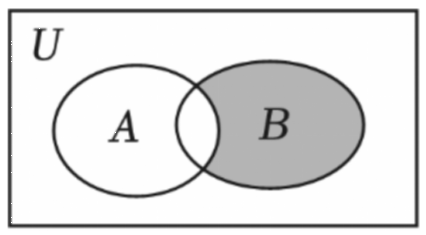
\includegraphics[width=0.26\textwidth]{figures/gao76_q14_venn.png}
\end{center}

\keepwithprev
A. $\{x\mid-2\leqslant x<4\}$\qquad B. $\{x\mid-1\leqslant x\leqslant3\}$

C. $\{x\mid x\leqslant3\text{ 或 }x\geqslant4\}$\qquad D. $\{x\mid-2\leqslant x\leqslant4\}$

\ifanswer
\solbegin
\step{全集 $U=\R$，集合 $A=\{x\mid x<-1\text{ 或 }x>4\}$，}
\step{$B=\{x\mid x^2-x-6\leqslant0\}=\{x\mid-2\leqslant x\leqslant3\}$，故 $A\cap B=\{x\mid-2\leqslant x<-1\}$，}
\step{故阴影部分表示的集合为 $\overline{A\cap B}=\{x\mid-1\leqslant x\leqslant3\}$. 故选 $B$.}
\solend
\fi

\item 设 $a$、$b$、$c\in\R$，给出下列命题：①若 $a>b$，则 $a^2>b^2$，②“$a>b$”是“$a^3>b^3$”的充要条件，③若 $a^2>b^2$，则 $|a|>|b|$，④若 $\dfrac ab>1$，则 $a>b$，⑤若 $a>b$，$c\neq0$，则 $\dfrac a{c^2}>\dfrac b{c^2}$，其中真命题的个数是\mbox{（\quad）}

\keepwithprev
A. $1$ 个\qquad B. $2$ 个\qquad C. $3$ 个\qquad D. $4$ 个

\ifanswer
\solbegin
\step{对于①，取 $a=2$，$b=-2$，满足 $a>b$，而 $a^2=b^2$，故为假命题；}
\step{对于②，$a>b\Leftrightarrow a^3-b^3=(a-b)(a^2+ab+b^2)=(a-b)\left[\left(a+\dfrac12b\right)^2+\dfrac34b^2\right]>0$}
\step{$\Leftrightarrow a^3>b^3$，故为真命题；}
\step{对于③，$a^2>b^2\Leftrightarrow|a|^2>|b|^2\Leftrightarrow|a|>|b|$，故为真命题；}
\step{对于④，取 $a=-2$，$b=-1$，满足 $\dfrac ab>1$，而 $a<b$，故为假命题；}
\step{对于⑤，由题意得 $c^2>0$，由 $a>b$，则 $\dfrac a{c^2}>\dfrac b{c^2}$，故为真命题.}
\step{故选 $C$.}
\solend
\fi

\item 已知关于 $x$ 的两个一元二次不等式 $a_1x^2+b_1x+c_1>0$，$a_2x^2+b_2x+c_2>0$ 的解集分别为 $A$、$B$，其中 $a_i$、$b_i$、$c_i(i=1,2)$ 为常数且不为零，则“$\dfrac{a_1}{a_2}=\dfrac{b_1}{b_2}=\dfrac{c_1}{c_2}$”是“$A=B$”\mbox{（\quad）}

\keepwithprev
A. 充分不必要条件\qquad B. 必要不充分条件

C. 充要条件\qquad D. 既不充分也不必要条件

\ifanswer
\solbegin
\step{设 $\dfrac{a_1}{a_2}=\dfrac{b_1}{b_2}=\dfrac{c_1}{c_2}=\lambda$，}
\step{①当 $\lambda>0$ 时，则 $a_1=\lambda a_2$，$b_1=\lambda b_2$，$c_1=\lambda c_2$，}
\step{$a_1x^2+b_1x+c_1>0\Leftrightarrow\lambda a_2x^2+\lambda b_2x+\lambda c_2>0\Leftrightarrow a_2x^2+b_2x+c_2>0$，}
\step{所以 $A=B$，}
\step{②当 $\lambda<0$ 时，则 $a_1=\lambda a_2$，$b_1=\lambda b_2$，$c_1=\lambda c_2$，}
\step{$a_1x^2+b_1x+c_1>0\Leftrightarrow\lambda a_2x^2+\lambda b_2x+\lambda c_2>0\Leftrightarrow a_2x^2+b_2x+c_2<0$，}
\step{所以 $A\neq B$，充分性不成立，}
\step{当 $A=B=\R$ 时，则 $\Delta<0$ 且 $a_1$、$a_2>0$，$\dfrac{a_1}{a_2}=\dfrac{b_1}{b_2}=\dfrac{c_1}{c_2}$ 不一定成立，}
\step{必要性不成立.}
\step{所以 $\dfrac{a_1}{a_2}=\dfrac{b_1}{b_2}=\dfrac{c_1}{c_2}$ 是 $A=B$ 的既不充分也不必要条件，故选 $D$.}
\solend
\fi

\end{enumerate}

\bigsec{三、解答题}

\begin{enumerate}
\setcounter{enumi}{16}

\item 求下列关于 $x$ 的不等式（组）的解集.

（1）$\begin{cases}9x^2-6x-24>0\\ \dfrac{x+3}{x-1}>2\end{cases}$；

（2）$|2x+1|-|2-x|>2$.

\ifanswer
\solbegin
\stepm{(1)}{不等式 $\dfrac{x+3}{x-1}>2$ 可化为 $\dfrac{x+3}{x-1}-2>0$，}
\step{即 $\dfrac{-x+5}{x-1}>0$，即 $(x-1)(x-5)<0$，解得 $1<x<5$，}
\step{不等式 $9x^2-6x-24>0$ 可化为 $(3x+4)(x-2)>0$，}
\step{解得 $x<-\dfrac43$ 或 $x>2$，}
\step{所以不等式的解集为 $(2,5)$.}
\stepm{(2)}{当 $x\leqslant-\dfrac12$ 时，$|2x+1|-|2-x|>2$ 等价于 $-2x-1-(2-x)>2$，}
\step{解得 $x<-5$，所以 $x<-5$，}
\step{当 $-\dfrac12<x<2$ 时，$|2x+1|-|2-x|>2$ 等价于 $2x+1-(2-x)>2$，}
\step{解得 $x>1$，所以 $1<x<2$，}
\step{当 $x\geqslant2$ 时，$|2x+1|-|2-x|>2$ 等价于 $2x+1-(x-2)>2$，}
\step{解得 $x>-1$，所以 $x\geqslant2$，}
\step{综上，$|2x+1|-|2-x|>2$ 的解集为 $(-\infty,-5)\cup(1,+\infty)$.}
\solend
\fi

\ansspace

\item 设 $m$ 为实数，求关于 $x$ 与 $y$ 的二元一次方程组 $\begin{cases}y=x+m\\ mx-y=4\end{cases}$ 的解集.

\ifanswer
\solbegin
\step{消去 $y$ 得 $(m-1)x=m+4$，}
\step{当 $m-1=0$，即 $m=1$ 时，$0=5$ 不成立，则 $x$ 无解，原方程组的解集为 $\varnothing$；}
\step{当 $m-1\neq0$，即 $m\neq1$ 时，则 $x=\dfrac{m+4}{m-1}$，$y=\dfrac{m+4}{m-1}+m=\dfrac{m^2+4}{m-1}$，}
\step{原方程组的解集为 $\left\{\left(\dfrac{m+4}{m-1},\dfrac{m^2+4}{m-1}\right)\right\}$.}
\step{综上所述，当 $m=1$ 时，方程组的解集为 $\varnothing$；}
\step{当 $m\neq1$ 时，方程组的解集为 $\left\{\left(\dfrac{m+4}{m-1},\dfrac{m^2+4}{m-1}\right)\right\}$.}
\solend
\fi

\ansspace

\item 已知集合 $A=\{x\mid-2\leqslant x-1\leqslant5\}$，集合 $B=\{x\mid m+1\leqslant x\leqslant2m-1\}(m\in\R)$.

（1）若 $m=4$，全集 $U=\R$，求 $A\cap B$；

（2）设命题 $p:x\in A$；命题 $q:x\in B$，若命题 $p$ 是命题 $q$ 的必要不充分条件，求实数 $m$ 的取值范围.

\ifanswer
\solbegin
\stepm{(1)}{由题意得 $A=\{x\mid-2\leqslant x-1\leqslant5\}=\{x\mid-1\leqslant x\leqslant6\}$，}
\step{当 $m=4$ 时，$B=\{x\mid5\leqslant x\leqslant7\}$，$A\cap B=\{x\mid5\leqslant x\leqslant6\}$；}
\stepm{(2)}{因为命题 $p$ 是命题 $q$ 的必要不充分条件，所以集合 $B$ 是集合 $A$ 的真子集，}
\step{当 $B=\varnothing$ 时，$m+1>2m-1$，解得 $m<2$，}
\step{当 $B\neq\varnothing$ 时，$\begin{cases}m+1\leqslant2m-1\\ m+1\geqslant-1\\ 2m-1\leqslant6\end{cases}$（等号不能同时成立），解得 $2\leqslant m\leqslant\dfrac72$，}
\step{综上所述，实数 $m$ 的取值范围为 $\left(-\infty,\dfrac72\right]$.}
\solend
\fi

\ansspace

\item （1）已知实数 $x\neq0$，求 $x+\dfrac1x$ 的取值范围；

（2）如图，要设计一张矩形海报，该海报含有大小相等的左右两个矩形栏目（即图中阴影部分），这两栏的面积之和为 $18000\,\mathrm{cm}^2$，四周空白的宽度为 $10\,\mathrm{cm}$，两栏之间的中缝空白的宽度为 $16\,\mathrm{cm}$，怎样确定海报的高与宽的尺寸（单位：$\mathrm{cm}$），能使矩形海报面积 $S$ 最小？最小面积是多少？

\begin{center}
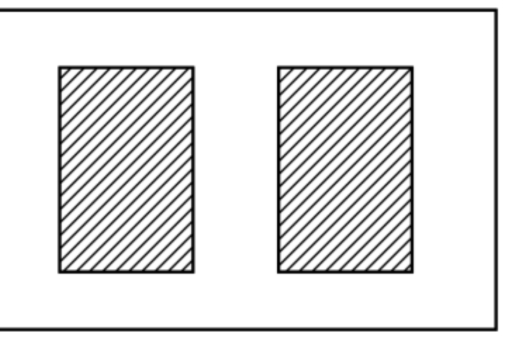
\includegraphics[width=0.34\textwidth]{figures/gao76_q20_poster.png}
\end{center}

\ifanswer
\solbegin
\stepm{(1)}{当 $x>0$ 时，$x+\dfrac1x\geqslant2\sqrt{x\times\dfrac1x}=2$，当且仅当 $x=\dfrac1x$，即 $x=1$ 取等号，}
\step{当 $x<0$ 时，$-x-\dfrac1x\geqslant2\sqrt{(-x)\times\dfrac1{-x}}=2$，所以 $x+\dfrac1x\leqslant-2$，}
\step{当且仅当 $-x=-\dfrac1x$，即 $x=-1$ 取等号，}
\step{综上所述，$x+\dfrac1x$ 的取值范围为 $(-\infty,-2]\cup[2,+\infty)$.}
\stepm{(2)}{设矩形栏目宽为 $x$，高为 $y$，则 $2xy=18000$，}
\step{所以 $S=(2x+36)(y+20)=2xy+36y+40x+720$}
% 原卷此行把 18720 写作 36720，照录（见文件头“原卷笔误/存疑”①）
\step{$=18000+36y+40x+720\geqslant18720+2\sqrt{36y\times40x}$}
\step{$=36720+2\sqrt{36\times40\times18000}=18720+7200=25920$，}
\step{当且仅当 $36y=40x$，即 $x=90$，$y=100$ 取等号，}
\step{所以海报的高为 $120\,\mathrm{cm}$ 与宽为 $216\,\mathrm{cm}$，可使矩形海报面积 $S$ 最小，}
\step{最小面积为 $25920$.}
\solend
\fi

\ansspace

\item 若实数 $x$、$y$、$m$ 满足 $|x-m|>|y-m|$，则称 $x$ 比 $y$ 远离 $m$.

（1）$0$ 比 $\dfrac12$ 远离 $2$ 吗？说明理由；

（2）若 $\dfrac1{2x-1}$ 比 $\dfrac12$ 远离 $1$，求实数 $x$ 的取值范围；

（3）若 $m\leqslant1$，$x+y=2$，试问：$x$ 与 $x^2+y^2$ 哪一个更远离 $m$，并说明理由.

\ifanswer
\solbegin
\stepm{(1)}{$0$ 比 $\dfrac12$ 远离 $2$，理由为：}
\step{由于 $|0-2|=2>\dfrac32=\left|\dfrac12-2\right|$，所以 $0$ 比 $\dfrac12$ 远离 $2$.}
\stepm{(2)}{由 $\dfrac1{2x-1}$ 比 $\dfrac12$ 远离 $1$，得 $\left|\dfrac1{2x-1}-1\right|>\left|\dfrac12-1\right|$，即 $\left|\dfrac1{2x-1}-1\right|>\dfrac12$，}
\step{则 $\dfrac1{2x-1}-1>\dfrac12$ 或 $\dfrac1{2x-1}-1<-\dfrac12$，整理得 $\dfrac1{2x-1}>\dfrac32$ 或 $\dfrac1{2x-1}<\dfrac12$，}
\step{因此 $0<2x-1<\dfrac23$ 或 $2x-1<0$ 或 $2x-1>2$，}
\step{解得 $\dfrac12<x<\dfrac56$ 或 $x<\dfrac12$ 或 $x>\dfrac32$，}
\step{所以 $x$ 的取值范围是 $\left(-\infty,\dfrac12\right)\cup\left(\dfrac12,\dfrac56\right)\cup\left(\dfrac32,+\infty\right)$.}
\stepm{(3)}{$x^2+y^2$ 比 $x$ 更远离 $m$，理由为：}
\step{由 $x^2+y^2\geqslant\dfrac{(x+y)^2}2=2\geqslant m$，得 $|x^2+y^2-m|=x^2+y^2-m$，}
\step{由 $x+y=2$，得 $x^2+y^2=x^2+(2-x)^2=2x^2-4x+4$，}
\step{于是 $|x^2+y^2-m|-|x-m|=2x^2-4x+4-m-|x-m|$，}
\step{当 $x\geqslant m$ 时，$|x^2+y^2-m|-|x-m|=2x^2-4x+4-m-(x-m)$}
\step{$=2\left(x-\dfrac54\right)^2+\dfrac78>0$，即 $|x^2+y^2-m|>|x-m|$；}
\step{当 $x<m$ 时，$|x^2+y^2-m|-|x-m|=2x^2-4x+4-m+(x-m)$}
\step{$=2\left(x-\dfrac34\right)^2+\dfrac{23}8-2m$，}
\step{由 $m\leqslant1$，得 $\dfrac{23}8-2m>0$，因此 $2\left(x-\dfrac34\right)^2+\dfrac{23}8-2m>0$，}
\step{即 $|x^2+y^2-m|>|x-m|$，}
\step{所以 $|x^2+y^2-m|>|x-m|$，即 $x^2+y^2$ 比 $x$ 更远离 $m$.}
\solend
\fi

\ansspace*[7]

\end{enumerate}

\end{document}
"
%
% 原始材料：微信公众号“魔都数学加油站”文章，连载“27学年高一76”；
% 原文标题“27学年高一76——2026-2027年上海市六十中学高一上10月月考”；
% 原文链接：https://mp.weixin.qq.com/s/GrKZjQrV1Xb0wy0BUuzAHw。
% 页面标注发布时间 2026-10-22 21:45（上海）。
% 正文为 10 张 PNG 页（`原图/高一76_六十中学_10月月考/01..10.png`）：
% 第 4、5、8、9 页为 4762×6735，其余 6 页为 2560×3620，均按页序读取。
% 10 页全为试卷正文页（卷首标题在第 1 页页顶，卷末第 21 题 (3) 解析止于第 10 页），
% 无封面页、目录页、二维码或宣传页。粉色斜排“魔都数学加油站”为卷面水印，未录入。
%
% 卷首标题：照卷面印作“2026-2027 年六十中学高一上 10 月月考”（黑体加粗一行）。
% 原卷年份区间用半角连字符，本稿按全稿惯例排 en dash；原卷无副标题。
%
% 篇幅与题号：原卷自第 3 题起编号（第 1、2 题不在本卷内）。填空题 3—12（10 题）、
% 选择题 13—16（4 题）、解答题 17—21（5 题），共 19 题。本稿沿用原节与原题号，
% 只改排为全稿统一的大节样式。
%
% 讲评版：原卷第 3、5 题只印【答案】（“$(0,1)$”“$a$、$b$ 都不能被 $3$ 整除”），
% 本稿只给 \ans{}；其余 17 题均印【解析】，用 \solbegin…\solend。四道选择题的作答
% 括号原卷即留空，答案写在解析末句“故选 C／B／C／D”，照录在解析内，不另提 \ans{}。
%
% 副标题：原卷未印副标题。本稿按“知识模块”口径标作“集合与常用逻辑用语、不等式”：
% 19 题中集合与常用逻辑用语 6 题（第 5、12、14、16、19 题及第 4 题的恒等变形），
% 不等式 13 题（第 3、6—11、13、15、17、18、20、21 题），两类均确有分量，故并标。
% 口径同 高一63、高一68—75。
%
% 与原卷的排版差异：
%   ① 原卷每题下直接印【答案】/【解析】，本稿按全稿惯例将答案与解析置于答案版；
%   ② 原卷未印副标题，本稿按“知识模块”口径补出；
%   ③ 原卷填空横线约四个字宽，本稿按全稿惯例统一排 \blankline[4.4em]；
%   ④ 原卷数集记号排斜体 $R$、$N$（第 4、6、7、8、11、12、14、15、19、20 题），本稿
%      按全稿惯例改用 $\R$、$\N$（同 高一68—75）；第 7、19、20 题的“解集为 $\R$”同此；
%   ⑤ 原卷句末标点多为西文句点，均逐处照录；
%   ⑥ 第 17—21 题的子问原卷印作“（1）…（2）…”，本稿按 高一69—75 成例用行内
%      “（1）（2）（3）”段，解析中的子问标号用 \stepm{(1)}{…}；
%   ⑦ 每道解答题原卷未留作答空白，本稿按全稿惯例加 \ansspace（末题用 \ansspace*）；
%   ⑧ 选择题的作答括号原卷排半角“(    )”，本稿按全稿惯例排 \mbox{（\quad）}；
%      选项行排照原卷——第 13、14、15、16 题一行两条、分两行排（本稿按原卷分行）；
%   ⑨ 第 10、11、17—21 题解析中的不等式组／方程组，原卷均排作“{”连接的多行式，
%      本稿按全稿惯例排 cases；
%   ⑩ 第 14 题题干右侧有一幅韦恩图（全集矩形内含 A、B 两圆，B 涂灰）：本稿按原卷
%      截图裁取（`figures/gao76_q14_venn.png`，由第 5 页原图裁出、去除粉色水印后转
%      灰度，未放大），放在题干之后、选项之前，仅答案版出；
%   ⑪ 第 20 题 (2) 题干右侧有一幅示意图（大矩形内两个斜线阴影小矩形）：本稿按原卷
%      截图裁取（`figures/gao76_q20_poster.png`，由第 8 页原图裁出、去除粉色水印后转
%      灰度，未放大），放在该小题文字之后，仅答案版出。
%
% 原卷笔误/存疑（均照录未改，正文对应处另有 % 注）：
%   ① 第 20 题 (2) 解析第 3 行把 $2xy+720$ 写成 $36720$（实为 $18000+720=18720$），
%      同式下一行又写回 $18720$，前后不一致；原卷如此，照录未改。
%   ② 第 14 题的韦恩图阴影是把整个 $B$ 圆（含 $A\cap B$ 部分）涂灰，而解析按
%      $\overline{A\cap B}$ 求解，二者不一致；原卷图文如此，照录未改。
%
% 行数核对：逐题数 \step/\stepm 条数与原卷【解析】印刷行数，17 题逐一相符，
% 合计 118 条 / 118 行（Q4：3；Q6：4；Q7：1；Q8：6；Q9：3；Q10：7；Q11：4；
% Q12：16；Q13：1；Q14：3；Q15：7；Q16：10；Q17：12；Q18：6；Q19：6；Q20：11；
% Q21：18）。另第 3、5 题只印【答案】，各提 \ans{}，不计入 \step 账。
%
% 插图：第 14 题题干的韦恩图、第 20 题 (2) 的示意图，见上⑩⑪；其余题干无配图。
%
\documentclass[a4paper,11pt]{article}
\usepackage{common}

\begin{document}

\examtitlest[3]{2026--2027 年六十中学高一上 10 月月考}{集合与常用逻辑用语、不等式}

\bigsec{一、填空题}

\begin{enumerate}
\setcounter{enumi}{2}

\item 不等式 $\dfrac{x}{1-x}>0$ 的解集是\blankline[4.4em].

\ifanswer
\ans{$(0,1)$}
\fi

\item 已知 $2x^2+x+1=a(x+1)^2+b(x+1)+2$，对 $x\in\R$ 恒成立，$ab=$\blankline[4.4em].

\ifanswer
\solbegin
\step{若 $2x^2+x+1=a(x+1)^2+b(x+1)+2$ 对 $x\in\R$ 恒成立，}
\step{即 $2x^2+x+1=ax^2+(2a+b)x+a+b+2$ 对 $x\in\R$ 恒成立，}
\step{必有 $\begin{cases}a=2\\ 2a+b=1\\ a+b+2=1\end{cases}$，解得 $a=2$，$b=-3$，所以 $ab=-6$.}
\solend
\fi

\item 利用反证法证明命题：“如果 $a$、$b\in\N$，$ab$ 可被 $3$ 整除，那么 $a$、$b$ 中至少有一个能被 $3$ 整除”时，假设的内容应是\blankline[4.4em].

\ifanswer
\ans{$a$、$b$ 都不能被 $3$ 整除}
\fi

\item 已知 $x\in\R$，方程 $|x+1|+|2-x|=3$ 的解集为\blankline[4.4em].

\ifanswer
\solbegin
\step{当 $x<-1$ 时，则 $|x+1|+|2-x|=-x-1+2-x=1-2x>3$；}
\step{当 $-1\leqslant x\leqslant2$ 时，则 $|x+1|+|2-x|=x+1+2-x=3$；}
\step{当 $x>2$ 时，则 $|x+1|+|2-x|=x+1+x-2=2x-1>3$.}
\step{综上所述，原方程的解集为 $[-1,2]$.}
\solend
\fi

\item 若关于 $x$ 的不等式 $x^2+kx+1\geqslant0$ 的解集为 $\R$，则实数 $k$ 的取值范围是\blankline[4.4em].

\ifanswer
\solbegin
\step{$\Delta=k^2-4\leqslant0\Rightarrow-2\leqslant k\leqslant2$，所以实数 $k$ 的取值范围是 $[-2,2]$.}
\solend
\fi

\item 已知 $a$、$b\in\R$，且 $ab>0$，则下列不等式中，恒成立的序号是\blankline[4.4em].

① $a^2+b^2>2ab$；② $a+b\geqslant2\sqrt{ab}$；③ $\dfrac1a+\dfrac1b>\dfrac2{\sqrt{ab}}$；④ $\dfrac ba+\dfrac ab\geqslant2$.

\ifanswer
\solbegin
\step{因为 $a^2+b^2\geqslant2ab$ 对于 $a$、$b\in\R$ 恒成立，当且仅当 $a=b$ 时取等号，}
\step{所以①错误；}
\step{对于②，③，显然 $a<0$，$b<0$ 时，不等式均不成立，即②和③错误；}
\step{对于④，因为 $ab>0$，所以 $\dfrac ba>0,\dfrac ab>0$，}
\step{由基本不等式得 $\dfrac ba+\dfrac ab\geqslant2\sqrt{\dfrac ba\cdot\dfrac ab}=2$，即④正确.}
\step{故正确的是④.}
\solend
\fi

\item 已知正实数 $m$、$n$ 满足 $m+\dfrac2n=1$，则 $\dfrac1m+2n$ 的最小值为\blankline[4.4em].

\ifanswer
\solbegin
\step{$\dfrac1m+2n=\left(m+\dfrac2n\right)\left(\dfrac1m+2n\right)=5+2mn+\dfrac2{mn}$，}
\step{因为 $mn>0$，所以 $2mn+\dfrac2{mn}\geqslant2\sqrt{2mn\cdot\dfrac2{mn}}=4$，}
\step{当且仅当 $2mn=\dfrac2{mn}$，即 $m=\dfrac13$，$n=3$ 时取等号，所以 $\dfrac1m+2n$ 的最小值为 $9$.}
\solend
\fi

\item 若关于 $x$ 的不等式组 $\begin{cases}3x+1>0\\ x+\dfrac1a\leqslant2\end{cases}$ 恰好有两个整数解，则实数 $a$ 的取值范围为\blankline[4.4em].

\ifanswer
\solbegin
\step{由 $3x+1>0$ 得 $x>-\dfrac13$；若 $a<0$，则 $\dfrac1a<0$，由 $x+\dfrac1a\leqslant2$ 得 $x\leqslant2-\dfrac1a>2$，}
\step{则解集 $\left(-\dfrac13,2-\dfrac1a\right]$ 必同时含有整数 $0$、$1$、$2$，不合题意；}
\step{又 $a=0$ 使 $\dfrac1a$ 无意义，故 $a>0$；}
\step{此时原不等式组的解集为 $\left(-\dfrac13,2-\dfrac1a\right]$，}
\step{其中大于 $-\dfrac13$ 的整数依次为 $0$，$1$，$2$，$\cdots$，}
\step{恰有两个整数解即解集只含 $0$ 与 $1$，故 $1\leqslant2-\dfrac1a<2$，即 $\dfrac1a\leqslant1$ 且 $\dfrac1a>0$，}
\step{结合 $a>0$，解得 $a\geqslant1$.}
\solend
\fi

\item 已知 $a\in\R$，若关于 $x$ 的方程 $x^2+ax+a^2-8=0$ 有两个实根 $x_1$、$x_2$，且 $\dfrac1{x_1}+\dfrac1{x_2}=-\dfrac12$，则 $a$ 的值为\blankline[4.4em].

\ifanswer
\solbegin
\step{由题意得 $\Delta=a^2-4(a^2-8)=32-3a^2\geqslant0$，解得 $a^2\leqslant\dfrac{32}3$，}
\step{由韦达定理得 $x_1+x_2=-a$，$x_1x_2=a^2-8$，}
\step{则 $\dfrac1{x_1}+\dfrac1{x_2}=\dfrac{x_1+x_2}{x_1x_2}=\dfrac{-a}{a^2-8}=-\dfrac12$，即 $a^2-2a-8=(a-4)(a+2)=0$，}
\step{解得 $a=4$ 或 $a=-2$，又 $a^2\leqslant\dfrac{32}3$，则 $a=-2$.}
\solend
\fi

\item 已知有限集 $A=\{a_1,a_2,\cdots,a_n\}(n\geqslant2,n\in\N)$，若 $A$ 中元素 $a_i(i=1,2,\cdots,n)$ 满足 $a_1+a_2+\cdots+a_n=a_1\times a_2\times\cdots\times a_n$，就称 $A$ 为“完美集”，以下四个命题：

①集合 $\{-1-\sqrt3,-1+\sqrt3\}$ 不是“完美集”；

②若 $a_1$、$a_2$ 是两个不同的正数，且 $\{a_1,a_2\}$ 是“完美集”，则 $a_1$、$a_2$ 至少有一个大于 $2$；

③二元“完美集”有无穷多个；

④若 $a_i$ 均为正整数，则“完美集”$A$ 有且只有一个，且 $n=3$.

其中，真命题的序号是\blankline[4.4em].

\ifanswer
\solbegin
\step{对于①选项：$(-1-\sqrt3)+(-1+\sqrt3)=-2$，$(-1-\sqrt3)\times(-1+\sqrt3)=-2$，}
\step{故 $(-1-\sqrt3)+(-1+\sqrt3)=(-1-\sqrt3)\times(-1+\sqrt3)$，}
\step{所以集合 $\{-1-\sqrt3,-1+\sqrt3\}$ 是“完美集”，故①错误；}
\step{对于②选项：集合 $\{a_1,a_2\}$ 是“完美集”，设 $a_1+a_2=a_1a_2=t>0$，}
\step{则 $a_1$、$a_2$ 可以看成一元二次方程 $x^2-tx+t=0$ 的两正根，则 $\Delta=t^2-4t>0$，}
\step{解得 $t<0$（舍）或 $t>4$，即 $a_1a_2>4$，所以至少有一个大于 $2$，故②正确；}
\step{对于③选项：由②得一元二次方程 $x^2-tx+t=0$ 当 $t$ 取不同值时，}
\step{$a_1$、$a_2$ 的值是不同的，因而二元“完美集”有无穷多个，故③正确；}
\step{对于④选项：设 $a_1<a_2<a_3<\cdots<a_n$，}
\step{则 $a_1\times a_2\times\cdots\times a_n=a_1+a_2+\cdots+a_n<na_n$，}
\step{所以 $a_1\times a_2\times\cdots\times a_{n-1}<n$，又 $a_i\in\N^*$，所以 $n\leqslant3$，}
\step{当 $n=2$ 时，$a_1<2$，则 $a_1=1$，$a_1a_2\neq a_1+a_2$，不合题意，}
\step{当 $n=3$ 时，$a_1a_2<3$，所以只能是 $a_1=1$，$a_2=2$，}
\step{由 $a_1+a_2+a_3=a_1a_2a_3$，代入解得 $a_3=3$，所以此时“完美集”只有一个，}
\step{为 $\{1,2,3\}$，故④正确.}
\step{故正确的是②③④.}
\solend
\fi

\end{enumerate}

\bigsec{二、选择题}

\begin{enumerate}
\setcounter{enumi}{12}

\item 已知 $x$、$y\in\R$，则“$xy\geqslant0$”是“$xy=|xy|$”的\mbox{（\quad）}

\keepwithprev
A. 充分非必要条件\qquad B. 必要非充分条件

C. 充要条件\qquad D. 既非充分也非必要条件

\ifanswer
\solbegin
\step{$xy\geqslant0\Leftrightarrow xy=|xy|$，故“$xy\geqslant0$”是“$xy=|xy|$”的充要条件. 故选 $C$.}
\solend
\fi

\needvspace{22\baselineskip}
\item 已知全集 $U=\R$，集合 $A=\{x\mid x<-1\text{ 或 }x>4\}$，$B=\{x\mid x^2-x-6\leqslant0\}$，则阴影部分表示的集合为\mbox{（\quad）}

\begin{center}
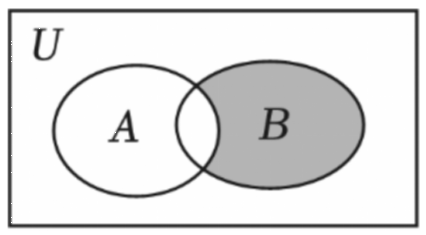
\includegraphics[width=0.26\textwidth]{figures/gao76_q14_venn.png}
\end{center}

\keepwithprev
A. $\{x\mid-2\leqslant x<4\}$\qquad B. $\{x\mid-1\leqslant x\leqslant3\}$

C. $\{x\mid x\leqslant3\text{ 或 }x\geqslant4\}$\qquad D. $\{x\mid-2\leqslant x\leqslant4\}$

\ifanswer
\solbegin
\step{全集 $U=\R$，集合 $A=\{x\mid x<-1\text{ 或 }x>4\}$，}
\step{$B=\{x\mid x^2-x-6\leqslant0\}=\{x\mid-2\leqslant x\leqslant3\}$，故 $A\cap B=\{x\mid-2\leqslant x<-1\}$，}
\step{故阴影部分表示的集合为 $\overline{A\cap B}=\{x\mid-1\leqslant x\leqslant3\}$. 故选 $B$.}
\solend
\fi

\item 设 $a$、$b$、$c\in\R$，给出下列命题：①若 $a>b$，则 $a^2>b^2$，②“$a>b$”是“$a^3>b^3$”的充要条件，③若 $a^2>b^2$，则 $|a|>|b|$，④若 $\dfrac ab>1$，则 $a>b$，⑤若 $a>b$，$c\neq0$，则 $\dfrac a{c^2}>\dfrac b{c^2}$，其中真命题的个数是\mbox{（\quad）}

\keepwithprev
A. $1$ 个\qquad B. $2$ 个\qquad C. $3$ 个\qquad D. $4$ 个

\ifanswer
\solbegin
\step{对于①，取 $a=2$，$b=-2$，满足 $a>b$，而 $a^2=b^2$，故为假命题；}
\step{对于②，$a>b\Leftrightarrow a^3-b^3=(a-b)(a^2+ab+b^2)=(a-b)\left[\left(a+\dfrac12b\right)^2+\dfrac34b^2\right]>0$}
\step{$\Leftrightarrow a^3>b^3$，故为真命题；}
\step{对于③，$a^2>b^2\Leftrightarrow|a|^2>|b|^2\Leftrightarrow|a|>|b|$，故为真命题；}
\step{对于④，取 $a=-2$，$b=-1$，满足 $\dfrac ab>1$，而 $a<b$，故为假命题；}
\step{对于⑤，由题意得 $c^2>0$，由 $a>b$，则 $\dfrac a{c^2}>\dfrac b{c^2}$，故为真命题.}
\step{故选 $C$.}
\solend
\fi

\item 已知关于 $x$ 的两个一元二次不等式 $a_1x^2+b_1x+c_1>0$，$a_2x^2+b_2x+c_2>0$ 的解集分别为 $A$、$B$，其中 $a_i$、$b_i$、$c_i(i=1,2)$ 为常数且不为零，则“$\dfrac{a_1}{a_2}=\dfrac{b_1}{b_2}=\dfrac{c_1}{c_2}$”是“$A=B$”\mbox{（\quad）}

\keepwithprev
A. 充分不必要条件\qquad B. 必要不充分条件

C. 充要条件\qquad D. 既不充分也不必要条件

\ifanswer
\solbegin
\step{设 $\dfrac{a_1}{a_2}=\dfrac{b_1}{b_2}=\dfrac{c_1}{c_2}=\lambda$，}
\step{①当 $\lambda>0$ 时，则 $a_1=\lambda a_2$，$b_1=\lambda b_2$，$c_1=\lambda c_2$，}
\step{$a_1x^2+b_1x+c_1>0\Leftrightarrow\lambda a_2x^2+\lambda b_2x+\lambda c_2>0\Leftrightarrow a_2x^2+b_2x+c_2>0$，}
\step{所以 $A=B$，}
\step{②当 $\lambda<0$ 时，则 $a_1=\lambda a_2$，$b_1=\lambda b_2$，$c_1=\lambda c_2$，}
\step{$a_1x^2+b_1x+c_1>0\Leftrightarrow\lambda a_2x^2+\lambda b_2x+\lambda c_2>0\Leftrightarrow a_2x^2+b_2x+c_2<0$，}
\step{所以 $A\neq B$，充分性不成立，}
\step{当 $A=B=\R$ 时，则 $\Delta<0$ 且 $a_1$、$a_2>0$，$\dfrac{a_1}{a_2}=\dfrac{b_1}{b_2}=\dfrac{c_1}{c_2}$ 不一定成立，}
\step{必要性不成立.}
\step{所以 $\dfrac{a_1}{a_2}=\dfrac{b_1}{b_2}=\dfrac{c_1}{c_2}$ 是 $A=B$ 的既不充分也不必要条件，故选 $D$.}
\solend
\fi

\end{enumerate}

\bigsec{三、解答题}

\begin{enumerate}
\setcounter{enumi}{16}

\item 求下列关于 $x$ 的不等式（组）的解集.

（1）$\begin{cases}9x^2-6x-24>0\\ \dfrac{x+3}{x-1}>2\end{cases}$；

（2）$|2x+1|-|2-x|>2$.

\ifanswer
\solbegin
\stepm{(1)}{不等式 $\dfrac{x+3}{x-1}>2$ 可化为 $\dfrac{x+3}{x-1}-2>0$，}
\step{即 $\dfrac{-x+5}{x-1}>0$，即 $(x-1)(x-5)<0$，解得 $1<x<5$，}
\step{不等式 $9x^2-6x-24>0$ 可化为 $(3x+4)(x-2)>0$，}
\step{解得 $x<-\dfrac43$ 或 $x>2$，}
\step{所以不等式的解集为 $(2,5)$.}
\stepm{(2)}{当 $x\leqslant-\dfrac12$ 时，$|2x+1|-|2-x|>2$ 等价于 $-2x-1-(2-x)>2$，}
\step{解得 $x<-5$，所以 $x<-5$，}
\step{当 $-\dfrac12<x<2$ 时，$|2x+1|-|2-x|>2$ 等价于 $2x+1-(2-x)>2$，}
\step{解得 $x>1$，所以 $1<x<2$，}
\step{当 $x\geqslant2$ 时，$|2x+1|-|2-x|>2$ 等价于 $2x+1-(x-2)>2$，}
\step{解得 $x>-1$，所以 $x\geqslant2$，}
\step{综上，$|2x+1|-|2-x|>2$ 的解集为 $(-\infty,-5)\cup(1,+\infty)$.}
\solend
\fi

\ansspace

\item 设 $m$ 为实数，求关于 $x$ 与 $y$ 的二元一次方程组 $\begin{cases}y=x+m\\ mx-y=4\end{cases}$ 的解集.

\ifanswer
\solbegin
\step{消去 $y$ 得 $(m-1)x=m+4$，}
\step{当 $m-1=0$，即 $m=1$ 时，$0=5$ 不成立，则 $x$ 无解，原方程组的解集为 $\varnothing$；}
\step{当 $m-1\neq0$，即 $m\neq1$ 时，则 $x=\dfrac{m+4}{m-1}$，$y=\dfrac{m+4}{m-1}+m=\dfrac{m^2+4}{m-1}$，}
\step{原方程组的解集为 $\left\{\left(\dfrac{m+4}{m-1},\dfrac{m^2+4}{m-1}\right)\right\}$.}
\step{综上所述，当 $m=1$ 时，方程组的解集为 $\varnothing$；}
\step{当 $m\neq1$ 时，方程组的解集为 $\left\{\left(\dfrac{m+4}{m-1},\dfrac{m^2+4}{m-1}\right)\right\}$.}
\solend
\fi

\ansspace

\item 已知集合 $A=\{x\mid-2\leqslant x-1\leqslant5\}$，集合 $B=\{x\mid m+1\leqslant x\leqslant2m-1\}(m\in\R)$.

（1）若 $m=4$，全集 $U=\R$，求 $A\cap B$；

（2）设命题 $p:x\in A$；命题 $q:x\in B$，若命题 $p$ 是命题 $q$ 的必要不充分条件，求实数 $m$ 的取值范围.

\ifanswer
\solbegin
\stepm{(1)}{由题意得 $A=\{x\mid-2\leqslant x-1\leqslant5\}=\{x\mid-1\leqslant x\leqslant6\}$，}
\step{当 $m=4$ 时，$B=\{x\mid5\leqslant x\leqslant7\}$，$A\cap B=\{x\mid5\leqslant x\leqslant6\}$；}
\stepm{(2)}{因为命题 $p$ 是命题 $q$ 的必要不充分条件，所以集合 $B$ 是集合 $A$ 的真子集，}
\step{当 $B=\varnothing$ 时，$m+1>2m-1$，解得 $m<2$，}
\step{当 $B\neq\varnothing$ 时，$\begin{cases}m+1\leqslant2m-1\\ m+1\geqslant-1\\ 2m-1\leqslant6\end{cases}$（等号不能同时成立），解得 $2\leqslant m\leqslant\dfrac72$，}
\step{综上所述，实数 $m$ 的取值范围为 $\left(-\infty,\dfrac72\right]$.}
\solend
\fi

\ansspace

\item （1）已知实数 $x\neq0$，求 $x+\dfrac1x$ 的取值范围；

（2）如图，要设计一张矩形海报，该海报含有大小相等的左右两个矩形栏目（即图中阴影部分），这两栏的面积之和为 $18000\,\mathrm{cm}^2$，四周空白的宽度为 $10\,\mathrm{cm}$，两栏之间的中缝空白的宽度为 $16\,\mathrm{cm}$，怎样确定海报的高与宽的尺寸（单位：$\mathrm{cm}$），能使矩形海报面积 $S$ 最小？最小面积是多少？

\begin{center}
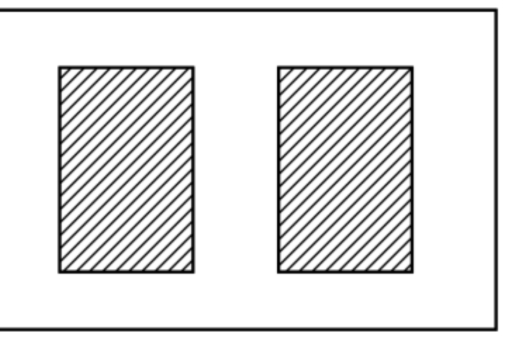
\includegraphics[width=0.34\textwidth]{figures/gao76_q20_poster.png}
\end{center}

\ifanswer
\solbegin
\stepm{(1)}{当 $x>0$ 时，$x+\dfrac1x\geqslant2\sqrt{x\times\dfrac1x}=2$，当且仅当 $x=\dfrac1x$，即 $x=1$ 取等号，}
\step{当 $x<0$ 时，$-x-\dfrac1x\geqslant2\sqrt{(-x)\times\dfrac1{-x}}=2$，所以 $x+\dfrac1x\leqslant-2$，}
\step{当且仅当 $-x=-\dfrac1x$，即 $x=-1$ 取等号，}
\step{综上所述，$x+\dfrac1x$ 的取值范围为 $(-\infty,-2]\cup[2,+\infty)$.}
\stepm{(2)}{设矩形栏目宽为 $x$，高为 $y$，则 $2xy=18000$，}
\step{所以 $S=(2x+36)(y+20)=2xy+36y+40x+720$}
% 原卷此行把 18720 写作 36720，照录（见文件头“原卷笔误/存疑”①）
\step{$=18000+36y+40x+720\geqslant18720+2\sqrt{36y\times40x}$}
\step{$=36720+2\sqrt{36\times40\times18000}=18720+7200=25920$，}
\step{当且仅当 $36y=40x$，即 $x=90$，$y=100$ 取等号，}
\step{所以海报的高为 $120\,\mathrm{cm}$ 与宽为 $216\,\mathrm{cm}$，可使矩形海报面积 $S$ 最小，}
\step{最小面积为 $25920$.}
\solend
\fi

\ansspace

\item 若实数 $x$、$y$、$m$ 满足 $|x-m|>|y-m|$，则称 $x$ 比 $y$ 远离 $m$.

（1）$0$ 比 $\dfrac12$ 远离 $2$ 吗？说明理由；

（2）若 $\dfrac1{2x-1}$ 比 $\dfrac12$ 远离 $1$，求实数 $x$ 的取值范围；

（3）若 $m\leqslant1$，$x+y=2$，试问：$x$ 与 $x^2+y^2$ 哪一个更远离 $m$，并说明理由.

\ifanswer
\solbegin
\stepm{(1)}{$0$ 比 $\dfrac12$ 远离 $2$，理由为：}
\step{由于 $|0-2|=2>\dfrac32=\left|\dfrac12-2\right|$，所以 $0$ 比 $\dfrac12$ 远离 $2$.}
\stepm{(2)}{由 $\dfrac1{2x-1}$ 比 $\dfrac12$ 远离 $1$，得 $\left|\dfrac1{2x-1}-1\right|>\left|\dfrac12-1\right|$，即 $\left|\dfrac1{2x-1}-1\right|>\dfrac12$，}
\step{则 $\dfrac1{2x-1}-1>\dfrac12$ 或 $\dfrac1{2x-1}-1<-\dfrac12$，整理得 $\dfrac1{2x-1}>\dfrac32$ 或 $\dfrac1{2x-1}<\dfrac12$，}
\step{因此 $0<2x-1<\dfrac23$ 或 $2x-1<0$ 或 $2x-1>2$，}
\step{解得 $\dfrac12<x<\dfrac56$ 或 $x<\dfrac12$ 或 $x>\dfrac32$，}
\step{所以 $x$ 的取值范围是 $\left(-\infty,\dfrac12\right)\cup\left(\dfrac12,\dfrac56\right)\cup\left(\dfrac32,+\infty\right)$.}
\stepm{(3)}{$x^2+y^2$ 比 $x$ 更远离 $m$，理由为：}
\step{由 $x^2+y^2\geqslant\dfrac{(x+y)^2}2=2\geqslant m$，得 $|x^2+y^2-m|=x^2+y^2-m$，}
\step{由 $x+y=2$，得 $x^2+y^2=x^2+(2-x)^2=2x^2-4x+4$，}
\step{于是 $|x^2+y^2-m|-|x-m|=2x^2-4x+4-m-|x-m|$，}
\step{当 $x\geqslant m$ 时，$|x^2+y^2-m|-|x-m|=2x^2-4x+4-m-(x-m)$}
\step{$=2\left(x-\dfrac54\right)^2+\dfrac78>0$，即 $|x^2+y^2-m|>|x-m|$；}
\step{当 $x<m$ 时，$|x^2+y^2-m|-|x-m|=2x^2-4x+4-m+(x-m)$}
\step{$=2\left(x-\dfrac34\right)^2+\dfrac{23}8-2m$，}
\step{由 $m\leqslant1$，得 $\dfrac{23}8-2m>0$，因此 $2\left(x-\dfrac34\right)^2+\dfrac{23}8-2m>0$，}
\step{即 $|x^2+y^2-m|>|x-m|$，}
\step{所以 $|x^2+y^2-m|>|x-m|$，即 $x^2+y^2$ 比 $x$ 更远离 $m$.}
\solend
\fi

\ansspace*[7]

\end{enumerate}

\end{document}
"
%
% 原始材料：微信公众号“魔都数学加油站”文章，连载“27学年高一76”；
% 原文标题“27学年高一76——2026-2027年上海市六十中学高一上10月月考”；
% 原文链接：https://mp.weixin.qq.com/s/GrKZjQrV1Xb0wy0BUuzAHw。
% 页面标注发布时间 2026-10-22 21:45（上海）。
% 正文为 10 张 PNG 页（`原图/高一76_六十中学_10月月考/01..10.png`）：
% 第 4、5、8、9 页为 4762×6735，其余 6 页为 2560×3620，均按页序读取。
% 10 页全为试卷正文页（卷首标题在第 1 页页顶，卷末第 21 题 (3) 解析止于第 10 页），
% 无封面页、目录页、二维码或宣传页。粉色斜排“魔都数学加油站”为卷面水印，未录入。
%
% 卷首标题：照卷面印作“2026-2027 年六十中学高一上 10 月月考”（黑体加粗一行）。
% 原卷年份区间用半角连字符，本稿按全稿惯例排 en dash；原卷无副标题。
%
% 篇幅与题号：原卷自第 3 题起编号（第 1、2 题不在本卷内）。填空题 3—12（10 题）、
% 选择题 13—16（4 题）、解答题 17—21（5 题），共 19 题。本稿沿用原节与原题号，
% 只改排为全稿统一的大节样式。
%
% 讲评版：原卷第 3、5 题只印【答案】（“$(0,1)$”“$a$、$b$ 都不能被 $3$ 整除”），
% 本稿只给 \ans{}；其余 17 题均印【解析】，用 \solbegin…\solend。四道选择题的作答
% 括号原卷即留空，答案写在解析末句“故选 C／B／C／D”，照录在解析内，不另提 \ans{}。
%
% 副标题：原卷未印副标题。本稿按“知识模块”口径标作“集合与常用逻辑用语、不等式”：
% 19 题中集合与常用逻辑用语 6 题（第 5、12、14、16、19 题及第 4 题的恒等变形），
% 不等式 13 题（第 3、6—11、13、15、17、18、20、21 题），两类均确有分量，故并标。
% 口径同 高一63、高一68—75。
%
% 与原卷的排版差异：
%   ① 原卷每题下直接印【答案】/【解析】，本稿按全稿惯例将答案与解析置于答案版；
%   ② 原卷未印副标题，本稿按“知识模块”口径补出；
%   ③ 原卷填空横线约四个字宽，本稿按全稿惯例统一排 \blankline[4.4em]；
%   ④ 原卷数集记号排斜体 $R$、$N$（第 4、6、7、8、11、12、14、15、19、20 题），本稿
%      按全稿惯例改用 $\R$、$\N$（同 高一68—75）；第 7、19、20 题的“解集为 $\R$”同此；
%   ⑤ 原卷句末标点多为西文句点，均逐处照录；
%   ⑥ 第 17—21 题的子问原卷印作“（1）…（2）…”，本稿按 高一69—75 成例用行内
%      “（1）（2）（3）”段，解析中的子问标号用 \stepm{(1)}{…}；
%   ⑦ 每道解答题原卷未留作答空白，本稿按全稿惯例加 \ansspace（末题用 \ansspace*）；
%   ⑧ 选择题的作答括号原卷排半角“(    )”，本稿按全稿惯例排 \mbox{（\quad）}；
%      选项行排照原卷——第 13、14、15、16 题一行两条、分两行排（本稿按原卷分行）；
%   ⑨ 第 10、11、17—21 题解析中的不等式组／方程组，原卷均排作“{”连接的多行式，
%      本稿按全稿惯例排 cases；
%   ⑩ 第 14 题题干右侧有一幅韦恩图（全集矩形内含 A、B 两圆，B 涂灰）：本稿按原卷
%      截图裁取（`figures/gao76_q14_venn.png`，由第 5 页原图裁出、去除粉色水印后转
%      灰度，未放大），放在题干之后、选项之前，仅答案版出；
%   ⑪ 第 20 题 (2) 题干右侧有一幅示意图（大矩形内两个斜线阴影小矩形）：本稿按原卷
%      截图裁取（`figures/gao76_q20_poster.png`，由第 8 页原图裁出、去除粉色水印后转
%      灰度，未放大），放在该小题文字之后，仅答案版出。
%
% 原卷笔误/存疑（均照录未改，正文对应处另有 % 注）：
%   ① 第 20 题 (2) 解析第 3 行把 $2xy+720$ 写成 $36720$（实为 $18000+720=18720$），
%      同式下一行又写回 $18720$，前后不一致；原卷如此，照录未改。
%   ② 第 14 题的韦恩图阴影是把整个 $B$ 圆（含 $A\cap B$ 部分）涂灰，而解析按
%      $\overline{A\cap B}$ 求解，二者不一致；原卷图文如此，照录未改。
%
% 行数核对：逐题数 \step/\stepm 条数与原卷【解析】印刷行数，17 题逐一相符，
% 合计 118 条 / 118 行（Q4：3；Q6：4；Q7：1；Q8：6；Q9：3；Q10：7；Q11：4；
% Q12：16；Q13：1；Q14：3；Q15：7；Q16：10；Q17：12；Q18：6；Q19：6；Q20：11；
% Q21：18）。另第 3、5 题只印【答案】，各提 \ans{}，不计入 \step 账。
%
% 插图：第 14 题题干的韦恩图、第 20 题 (2) 的示意图，见上⑩⑪；其余题干无配图。
%
\documentclass[a4paper,11pt]{article}
\usepackage{common}

\begin{document}

\examtitlest[3]{2026--2027 年六十中学高一上 10 月月考}{集合与常用逻辑用语、不等式}

\bigsec{一、填空题}

\begin{enumerate}
\setcounter{enumi}{2}

\item 不等式 $\dfrac{x}{1-x}>0$ 的解集是\blankline[4.4em].

\ifanswer
\ans{$(0,1)$}
\fi

\item 已知 $2x^2+x+1=a(x+1)^2+b(x+1)+2$，对 $x\in\R$ 恒成立，$ab=$\blankline[4.4em].

\ifanswer
\solbegin
\step{若 $2x^2+x+1=a(x+1)^2+b(x+1)+2$ 对 $x\in\R$ 恒成立，}
\step{即 $2x^2+x+1=ax^2+(2a+b)x+a+b+2$ 对 $x\in\R$ 恒成立，}
\step{必有 $\begin{cases}a=2\\ 2a+b=1\\ a+b+2=1\end{cases}$，解得 $a=2$，$b=-3$，所以 $ab=-6$.}
\solend
\fi

\item 利用反证法证明命题：“如果 $a$、$b\in\N$，$ab$ 可被 $3$ 整除，那么 $a$、$b$ 中至少有一个能被 $3$ 整除”时，假设的内容应是\blankline[4.4em].

\ifanswer
\ans{$a$、$b$ 都不能被 $3$ 整除}
\fi

\item 已知 $x\in\R$，方程 $|x+1|+|2-x|=3$ 的解集为\blankline[4.4em].

\ifanswer
\solbegin
\step{当 $x<-1$ 时，则 $|x+1|+|2-x|=-x-1+2-x=1-2x>3$；}
\step{当 $-1\leqslant x\leqslant2$ 时，则 $|x+1|+|2-x|=x+1+2-x=3$；}
\step{当 $x>2$ 时，则 $|x+1|+|2-x|=x+1+x-2=2x-1>3$.}
\step{综上所述，原方程的解集为 $[-1,2]$.}
\solend
\fi

\item 若关于 $x$ 的不等式 $x^2+kx+1\geqslant0$ 的解集为 $\R$，则实数 $k$ 的取值范围是\blankline[4.4em].

\ifanswer
\solbegin
\step{$\Delta=k^2-4\leqslant0\Rightarrow-2\leqslant k\leqslant2$，所以实数 $k$ 的取值范围是 $[-2,2]$.}
\solend
\fi

\item 已知 $a$、$b\in\R$，且 $ab>0$，则下列不等式中，恒成立的序号是\blankline[4.4em].

① $a^2+b^2>2ab$；② $a+b\geqslant2\sqrt{ab}$；③ $\dfrac1a+\dfrac1b>\dfrac2{\sqrt{ab}}$；④ $\dfrac ba+\dfrac ab\geqslant2$.

\ifanswer
\solbegin
\step{因为 $a^2+b^2\geqslant2ab$ 对于 $a$、$b\in\R$ 恒成立，当且仅当 $a=b$ 时取等号，}
\step{所以①错误；}
\step{对于②，③，显然 $a<0$，$b<0$ 时，不等式均不成立，即②和③错误；}
\step{对于④，因为 $ab>0$，所以 $\dfrac ba>0,\dfrac ab>0$，}
\step{由基本不等式得 $\dfrac ba+\dfrac ab\geqslant2\sqrt{\dfrac ba\cdot\dfrac ab}=2$，即④正确.}
\step{故正确的是④.}
\solend
\fi

\item 已知正实数 $m$、$n$ 满足 $m+\dfrac2n=1$，则 $\dfrac1m+2n$ 的最小值为\blankline[4.4em].

\ifanswer
\solbegin
\step{$\dfrac1m+2n=\left(m+\dfrac2n\right)\left(\dfrac1m+2n\right)=5+2mn+\dfrac2{mn}$，}
\step{因为 $mn>0$，所以 $2mn+\dfrac2{mn}\geqslant2\sqrt{2mn\cdot\dfrac2{mn}}=4$，}
\step{当且仅当 $2mn=\dfrac2{mn}$，即 $m=\dfrac13$，$n=3$ 时取等号，所以 $\dfrac1m+2n$ 的最小值为 $9$.}
\solend
\fi

\item 若关于 $x$ 的不等式组 $\begin{cases}3x+1>0\\ x+\dfrac1a\leqslant2\end{cases}$ 恰好有两个整数解，则实数 $a$ 的取值范围为\blankline[4.4em].

\ifanswer
\solbegin
\step{由 $3x+1>0$ 得 $x>-\dfrac13$；若 $a<0$，则 $\dfrac1a<0$，由 $x+\dfrac1a\leqslant2$ 得 $x\leqslant2-\dfrac1a>2$，}
\step{则解集 $\left(-\dfrac13,2-\dfrac1a\right]$ 必同时含有整数 $0$、$1$、$2$，不合题意；}
\step{又 $a=0$ 使 $\dfrac1a$ 无意义，故 $a>0$；}
\step{此时原不等式组的解集为 $\left(-\dfrac13,2-\dfrac1a\right]$，}
\step{其中大于 $-\dfrac13$ 的整数依次为 $0$，$1$，$2$，$\cdots$，}
\step{恰有两个整数解即解集只含 $0$ 与 $1$，故 $1\leqslant2-\dfrac1a<2$，即 $\dfrac1a\leqslant1$ 且 $\dfrac1a>0$，}
\step{结合 $a>0$，解得 $a\geqslant1$.}
\solend
\fi

\item 已知 $a\in\R$，若关于 $x$ 的方程 $x^2+ax+a^2-8=0$ 有两个实根 $x_1$、$x_2$，且 $\dfrac1{x_1}+\dfrac1{x_2}=-\dfrac12$，则 $a$ 的值为\blankline[4.4em].

\ifanswer
\solbegin
\step{由题意得 $\Delta=a^2-4(a^2-8)=32-3a^2\geqslant0$，解得 $a^2\leqslant\dfrac{32}3$，}
\step{由韦达定理得 $x_1+x_2=-a$，$x_1x_2=a^2-8$，}
\step{则 $\dfrac1{x_1}+\dfrac1{x_2}=\dfrac{x_1+x_2}{x_1x_2}=\dfrac{-a}{a^2-8}=-\dfrac12$，即 $a^2-2a-8=(a-4)(a+2)=0$，}
\step{解得 $a=4$ 或 $a=-2$，又 $a^2\leqslant\dfrac{32}3$，则 $a=-2$.}
\solend
\fi

\item 已知有限集 $A=\{a_1,a_2,\cdots,a_n\}(n\geqslant2,n\in\N)$，若 $A$ 中元素 $a_i(i=1,2,\cdots,n)$ 满足 $a_1+a_2+\cdots+a_n=a_1\times a_2\times\cdots\times a_n$，就称 $A$ 为“完美集”，以下四个命题：

①集合 $\{-1-\sqrt3,-1+\sqrt3\}$ 不是“完美集”；

②若 $a_1$、$a_2$ 是两个不同的正数，且 $\{a_1,a_2\}$ 是“完美集”，则 $a_1$、$a_2$ 至少有一个大于 $2$；

③二元“完美集”有无穷多个；

④若 $a_i$ 均为正整数，则“完美集”$A$ 有且只有一个，且 $n=3$.

其中，真命题的序号是\blankline[4.4em].

\ifanswer
\solbegin
\step{对于①选项：$(-1-\sqrt3)+(-1+\sqrt3)=-2$，$(-1-\sqrt3)\times(-1+\sqrt3)=-2$，}
\step{故 $(-1-\sqrt3)+(-1+\sqrt3)=(-1-\sqrt3)\times(-1+\sqrt3)$，}
\step{所以集合 $\{-1-\sqrt3,-1+\sqrt3\}$ 是“完美集”，故①错误；}
\step{对于②选项：集合 $\{a_1,a_2\}$ 是“完美集”，设 $a_1+a_2=a_1a_2=t>0$，}
\step{则 $a_1$、$a_2$ 可以看成一元二次方程 $x^2-tx+t=0$ 的两正根，则 $\Delta=t^2-4t>0$，}
\step{解得 $t<0$（舍）或 $t>4$，即 $a_1a_2>4$，所以至少有一个大于 $2$，故②正确；}
\step{对于③选项：由②得一元二次方程 $x^2-tx+t=0$ 当 $t$ 取不同值时，}
\step{$a_1$、$a_2$ 的值是不同的，因而二元“完美集”有无穷多个，故③正确；}
\step{对于④选项：设 $a_1<a_2<a_3<\cdots<a_n$，}
\step{则 $a_1\times a_2\times\cdots\times a_n=a_1+a_2+\cdots+a_n<na_n$，}
\step{所以 $a_1\times a_2\times\cdots\times a_{n-1}<n$，又 $a_i\in\N^*$，所以 $n\leqslant3$，}
\step{当 $n=2$ 时，$a_1<2$，则 $a_1=1$，$a_1a_2\neq a_1+a_2$，不合题意，}
\step{当 $n=3$ 时，$a_1a_2<3$，所以只能是 $a_1=1$，$a_2=2$，}
\step{由 $a_1+a_2+a_3=a_1a_2a_3$，代入解得 $a_3=3$，所以此时“完美集”只有一个，}
\step{为 $\{1,2,3\}$，故④正确.}
\step{故正确的是②③④.}
\solend
\fi

\end{enumerate}

\bigsec{二、选择题}

\begin{enumerate}
\setcounter{enumi}{12}

\item 已知 $x$、$y\in\R$，则“$xy\geqslant0$”是“$xy=|xy|$”的\mbox{（\quad）}

\keepwithprev
A. 充分非必要条件\qquad B. 必要非充分条件

C. 充要条件\qquad D. 既非充分也非必要条件

\ifanswer
\solbegin
\step{$xy\geqslant0\Leftrightarrow xy=|xy|$，故“$xy\geqslant0$”是“$xy=|xy|$”的充要条件. 故选 $C$.}
\solend
\fi

\needvspace{22\baselineskip}
\item 已知全集 $U=\R$，集合 $A=\{x\mid x<-1\text{ 或 }x>4\}$，$B=\{x\mid x^2-x-6\leqslant0\}$，则阴影部分表示的集合为\mbox{（\quad）}

\begin{center}
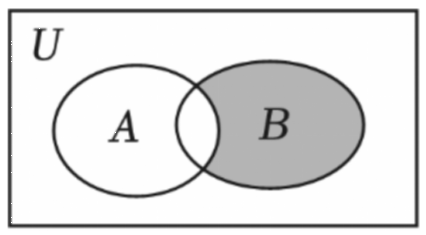
\includegraphics[width=0.26\textwidth]{figures/gao76_q14_venn.png}
\end{center}

\keepwithprev
A. $\{x\mid-2\leqslant x<4\}$\qquad B. $\{x\mid-1\leqslant x\leqslant3\}$

C. $\{x\mid x\leqslant3\text{ 或 }x\geqslant4\}$\qquad D. $\{x\mid-2\leqslant x\leqslant4\}$

\ifanswer
\solbegin
\step{全集 $U=\R$，集合 $A=\{x\mid x<-1\text{ 或 }x>4\}$，}
\step{$B=\{x\mid x^2-x-6\leqslant0\}=\{x\mid-2\leqslant x\leqslant3\}$，故 $A\cap B=\{x\mid-2\leqslant x<-1\}$，}
\step{故阴影部分表示的集合为 $\overline{A\cap B}=\{x\mid-1\leqslant x\leqslant3\}$. 故选 $B$.}
\solend
\fi

\item 设 $a$、$b$、$c\in\R$，给出下列命题：①若 $a>b$，则 $a^2>b^2$，②“$a>b$”是“$a^3>b^3$”的充要条件，③若 $a^2>b^2$，则 $|a|>|b|$，④若 $\dfrac ab>1$，则 $a>b$，⑤若 $a>b$，$c\neq0$，则 $\dfrac a{c^2}>\dfrac b{c^2}$，其中真命题的个数是\mbox{（\quad）}

\keepwithprev
A. $1$ 个\qquad B. $2$ 个\qquad C. $3$ 个\qquad D. $4$ 个

\ifanswer
\solbegin
\step{对于①，取 $a=2$，$b=-2$，满足 $a>b$，而 $a^2=b^2$，故为假命题；}
\step{对于②，$a>b\Leftrightarrow a^3-b^3=(a-b)(a^2+ab+b^2)=(a-b)\left[\left(a+\dfrac12b\right)^2+\dfrac34b^2\right]>0$}
\step{$\Leftrightarrow a^3>b^3$，故为真命题；}
\step{对于③，$a^2>b^2\Leftrightarrow|a|^2>|b|^2\Leftrightarrow|a|>|b|$，故为真命题；}
\step{对于④，取 $a=-2$，$b=-1$，满足 $\dfrac ab>1$，而 $a<b$，故为假命题；}
\step{对于⑤，由题意得 $c^2>0$，由 $a>b$，则 $\dfrac a{c^2}>\dfrac b{c^2}$，故为真命题.}
\step{故选 $C$.}
\solend
\fi

\item 已知关于 $x$ 的两个一元二次不等式 $a_1x^2+b_1x+c_1>0$，$a_2x^2+b_2x+c_2>0$ 的解集分别为 $A$、$B$，其中 $a_i$、$b_i$、$c_i(i=1,2)$ 为常数且不为零，则“$\dfrac{a_1}{a_2}=\dfrac{b_1}{b_2}=\dfrac{c_1}{c_2}$”是“$A=B$”\mbox{（\quad）}

\keepwithprev
A. 充分不必要条件\qquad B. 必要不充分条件

C. 充要条件\qquad D. 既不充分也不必要条件

\ifanswer
\solbegin
\step{设 $\dfrac{a_1}{a_2}=\dfrac{b_1}{b_2}=\dfrac{c_1}{c_2}=\lambda$，}
\step{①当 $\lambda>0$ 时，则 $a_1=\lambda a_2$，$b_1=\lambda b_2$，$c_1=\lambda c_2$，}
\step{$a_1x^2+b_1x+c_1>0\Leftrightarrow\lambda a_2x^2+\lambda b_2x+\lambda c_2>0\Leftrightarrow a_2x^2+b_2x+c_2>0$，}
\step{所以 $A=B$，}
\step{②当 $\lambda<0$ 时，则 $a_1=\lambda a_2$，$b_1=\lambda b_2$，$c_1=\lambda c_2$，}
\step{$a_1x^2+b_1x+c_1>0\Leftrightarrow\lambda a_2x^2+\lambda b_2x+\lambda c_2>0\Leftrightarrow a_2x^2+b_2x+c_2<0$，}
\step{所以 $A\neq B$，充分性不成立，}
\step{当 $A=B=\R$ 时，则 $\Delta<0$ 且 $a_1$、$a_2>0$，$\dfrac{a_1}{a_2}=\dfrac{b_1}{b_2}=\dfrac{c_1}{c_2}$ 不一定成立，}
\step{必要性不成立.}
\step{所以 $\dfrac{a_1}{a_2}=\dfrac{b_1}{b_2}=\dfrac{c_1}{c_2}$ 是 $A=B$ 的既不充分也不必要条件，故选 $D$.}
\solend
\fi

\end{enumerate}

\bigsec{三、解答题}

\begin{enumerate}
\setcounter{enumi}{16}

\item 求下列关于 $x$ 的不等式（组）的解集.

（1）$\begin{cases}9x^2-6x-24>0\\ \dfrac{x+3}{x-1}>2\end{cases}$；

（2）$|2x+1|-|2-x|>2$.

\ifanswer
\solbegin
\stepm{(1)}{不等式 $\dfrac{x+3}{x-1}>2$ 可化为 $\dfrac{x+3}{x-1}-2>0$，}
\step{即 $\dfrac{-x+5}{x-1}>0$，即 $(x-1)(x-5)<0$，解得 $1<x<5$，}
\step{不等式 $9x^2-6x-24>0$ 可化为 $(3x+4)(x-2)>0$，}
\step{解得 $x<-\dfrac43$ 或 $x>2$，}
\step{所以不等式的解集为 $(2,5)$.}
\stepm{(2)}{当 $x\leqslant-\dfrac12$ 时，$|2x+1|-|2-x|>2$ 等价于 $-2x-1-(2-x)>2$，}
\step{解得 $x<-5$，所以 $x<-5$，}
\step{当 $-\dfrac12<x<2$ 时，$|2x+1|-|2-x|>2$ 等价于 $2x+1-(2-x)>2$，}
\step{解得 $x>1$，所以 $1<x<2$，}
\step{当 $x\geqslant2$ 时，$|2x+1|-|2-x|>2$ 等价于 $2x+1-(x-2)>2$，}
\step{解得 $x>-1$，所以 $x\geqslant2$，}
\step{综上，$|2x+1|-|2-x|>2$ 的解集为 $(-\infty,-5)\cup(1,+\infty)$.}
\solend
\fi

\ansspace

\item 设 $m$ 为实数，求关于 $x$ 与 $y$ 的二元一次方程组 $\begin{cases}y=x+m\\ mx-y=4\end{cases}$ 的解集.

\ifanswer
\solbegin
\step{消去 $y$ 得 $(m-1)x=m+4$，}
\step{当 $m-1=0$，即 $m=1$ 时，$0=5$ 不成立，则 $x$ 无解，原方程组的解集为 $\varnothing$；}
\step{当 $m-1\neq0$，即 $m\neq1$ 时，则 $x=\dfrac{m+4}{m-1}$，$y=\dfrac{m+4}{m-1}+m=\dfrac{m^2+4}{m-1}$，}
\step{原方程组的解集为 $\left\{\left(\dfrac{m+4}{m-1},\dfrac{m^2+4}{m-1}\right)\right\}$.}
\step{综上所述，当 $m=1$ 时，方程组的解集为 $\varnothing$；}
\step{当 $m\neq1$ 时，方程组的解集为 $\left\{\left(\dfrac{m+4}{m-1},\dfrac{m^2+4}{m-1}\right)\right\}$.}
\solend
\fi

\ansspace

\item 已知集合 $A=\{x\mid-2\leqslant x-1\leqslant5\}$，集合 $B=\{x\mid m+1\leqslant x\leqslant2m-1\}(m\in\R)$.

（1）若 $m=4$，全集 $U=\R$，求 $A\cap B$；

（2）设命题 $p:x\in A$；命题 $q:x\in B$，若命题 $p$ 是命题 $q$ 的必要不充分条件，求实数 $m$ 的取值范围.

\ifanswer
\solbegin
\stepm{(1)}{由题意得 $A=\{x\mid-2\leqslant x-1\leqslant5\}=\{x\mid-1\leqslant x\leqslant6\}$，}
\step{当 $m=4$ 时，$B=\{x\mid5\leqslant x\leqslant7\}$，$A\cap B=\{x\mid5\leqslant x\leqslant6\}$；}
\stepm{(2)}{因为命题 $p$ 是命题 $q$ 的必要不充分条件，所以集合 $B$ 是集合 $A$ 的真子集，}
\step{当 $B=\varnothing$ 时，$m+1>2m-1$，解得 $m<2$，}
\step{当 $B\neq\varnothing$ 时，$\begin{cases}m+1\leqslant2m-1\\ m+1\geqslant-1\\ 2m-1\leqslant6\end{cases}$（等号不能同时成立），解得 $2\leqslant m\leqslant\dfrac72$，}
\step{综上所述，实数 $m$ 的取值范围为 $\left(-\infty,\dfrac72\right]$.}
\solend
\fi

\ansspace

\item （1）已知实数 $x\neq0$，求 $x+\dfrac1x$ 的取值范围；

（2）如图，要设计一张矩形海报，该海报含有大小相等的左右两个矩形栏目（即图中阴影部分），这两栏的面积之和为 $18000\,\mathrm{cm}^2$，四周空白的宽度为 $10\,\mathrm{cm}$，两栏之间的中缝空白的宽度为 $16\,\mathrm{cm}$，怎样确定海报的高与宽的尺寸（单位：$\mathrm{cm}$），能使矩形海报面积 $S$ 最小？最小面积是多少？

\begin{center}
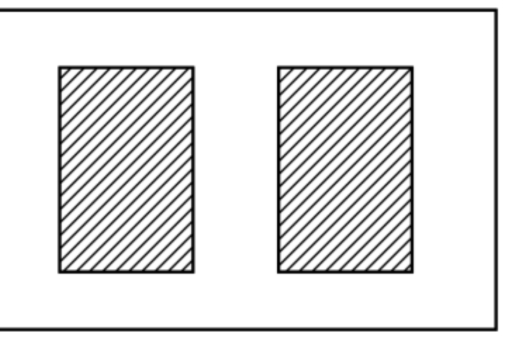
\includegraphics[width=0.34\textwidth]{figures/gao76_q20_poster.png}
\end{center}

\ifanswer
\solbegin
\stepm{(1)}{当 $x>0$ 时，$x+\dfrac1x\geqslant2\sqrt{x\times\dfrac1x}=2$，当且仅当 $x=\dfrac1x$，即 $x=1$ 取等号，}
\step{当 $x<0$ 时，$-x-\dfrac1x\geqslant2\sqrt{(-x)\times\dfrac1{-x}}=2$，所以 $x+\dfrac1x\leqslant-2$，}
\step{当且仅当 $-x=-\dfrac1x$，即 $x=-1$ 取等号，}
\step{综上所述，$x+\dfrac1x$ 的取值范围为 $(-\infty,-2]\cup[2,+\infty)$.}
\stepm{(2)}{设矩形栏目宽为 $x$，高为 $y$，则 $2xy=18000$，}
\step{所以 $S=(2x+36)(y+20)=2xy+36y+40x+720$}
% 原卷此行把 18720 写作 36720，照录（见文件头“原卷笔误/存疑”①）
\step{$=18000+36y+40x+720\geqslant18720+2\sqrt{36y\times40x}$}
\step{$=36720+2\sqrt{36\times40\times18000}=18720+7200=25920$，}
\step{当且仅当 $36y=40x$，即 $x=90$，$y=100$ 取等号，}
\step{所以海报的高为 $120\,\mathrm{cm}$ 与宽为 $216\,\mathrm{cm}$，可使矩形海报面积 $S$ 最小，}
\step{最小面积为 $25920$.}
\solend
\fi

\ansspace

\item 若实数 $x$、$y$、$m$ 满足 $|x-m|>|y-m|$，则称 $x$ 比 $y$ 远离 $m$.

（1）$0$ 比 $\dfrac12$ 远离 $2$ 吗？说明理由；

（2）若 $\dfrac1{2x-1}$ 比 $\dfrac12$ 远离 $1$，求实数 $x$ 的取值范围；

（3）若 $m\leqslant1$，$x+y=2$，试问：$x$ 与 $x^2+y^2$ 哪一个更远离 $m$，并说明理由.

\ifanswer
\solbegin
\stepm{(1)}{$0$ 比 $\dfrac12$ 远离 $2$，理由为：}
\step{由于 $|0-2|=2>\dfrac32=\left|\dfrac12-2\right|$，所以 $0$ 比 $\dfrac12$ 远离 $2$.}
\stepm{(2)}{由 $\dfrac1{2x-1}$ 比 $\dfrac12$ 远离 $1$，得 $\left|\dfrac1{2x-1}-1\right|>\left|\dfrac12-1\right|$，即 $\left|\dfrac1{2x-1}-1\right|>\dfrac12$，}
\step{则 $\dfrac1{2x-1}-1>\dfrac12$ 或 $\dfrac1{2x-1}-1<-\dfrac12$，整理得 $\dfrac1{2x-1}>\dfrac32$ 或 $\dfrac1{2x-1}<\dfrac12$，}
\step{因此 $0<2x-1<\dfrac23$ 或 $2x-1<0$ 或 $2x-1>2$，}
\step{解得 $\dfrac12<x<\dfrac56$ 或 $x<\dfrac12$ 或 $x>\dfrac32$，}
\step{所以 $x$ 的取值范围是 $\left(-\infty,\dfrac12\right)\cup\left(\dfrac12,\dfrac56\right)\cup\left(\dfrac32,+\infty\right)$.}
\stepm{(3)}{$x^2+y^2$ 比 $x$ 更远离 $m$，理由为：}
\step{由 $x^2+y^2\geqslant\dfrac{(x+y)^2}2=2\geqslant m$，得 $|x^2+y^2-m|=x^2+y^2-m$，}
\step{由 $x+y=2$，得 $x^2+y^2=x^2+(2-x)^2=2x^2-4x+4$，}
\step{于是 $|x^2+y^2-m|-|x-m|=2x^2-4x+4-m-|x-m|$，}
\step{当 $x\geqslant m$ 时，$|x^2+y^2-m|-|x-m|=2x^2-4x+4-m-(x-m)$}
\step{$=2\left(x-\dfrac54\right)^2+\dfrac78>0$，即 $|x^2+y^2-m|>|x-m|$；}
\step{当 $x<m$ 时，$|x^2+y^2-m|-|x-m|=2x^2-4x+4-m+(x-m)$}
\step{$=2\left(x-\dfrac34\right)^2+\dfrac{23}8-2m$，}
\step{由 $m\leqslant1$，得 $\dfrac{23}8-2m>0$，因此 $2\left(x-\dfrac34\right)^2+\dfrac{23}8-2m>0$，}
\step{即 $|x^2+y^2-m|>|x-m|$，}
\step{所以 $|x^2+y^2-m|>|x-m|$，即 $x^2+y^2$ 比 $x$ 更远离 $m$.}
\solend
\fi

\ansspace*[7]

\end{enumerate}

\end{document}
"
% 紧凑版：xelatex "\def\iscompact{1}% 高一76_六十中学_10月月考.tex
%   —— 高一上数学“2026-2027 年六十中学高一上 10 月月考”（讲评版）
% 试卷版：xelatex 高一76_六十中学_10月月考.tex
% 答案版：xelatex "\def\isanswer{1}% 高一76_六十中学_10月月考.tex
%   —— 高一上数学“2026-2027 年六十中学高一上 10 月月考”（讲评版）
% 试卷版：xelatex 高一76_六十中学_10月月考.tex
% 答案版：xelatex "\def\isanswer{1}% 高一76_六十中学_10月月考.tex
%   —— 高一上数学“2026-2027 年六十中学高一上 10 月月考”（讲评版）
% 试卷版：xelatex 高一76_六十中学_10月月考.tex
% 答案版：xelatex "\def\isanswer{1}\input{高一76_六十中学_10月月考.tex}"
% 紧凑版：xelatex "\def\iscompact{1}\input{高一76_六十中学_10月月考.tex}"
%
% 原始材料：微信公众号“魔都数学加油站”文章，连载“27学年高一76”；
% 原文标题“27学年高一76——2026-2027年上海市六十中学高一上10月月考”；
% 原文链接：https://mp.weixin.qq.com/s/GrKZjQrV1Xb0wy0BUuzAHw。
% 页面标注发布时间 2026-10-22 21:45（上海）。
% 正文为 10 张 PNG 页（`原图/高一76_六十中学_10月月考/01..10.png`）：
% 第 4、5、8、9 页为 4762×6735，其余 6 页为 2560×3620，均按页序读取。
% 10 页全为试卷正文页（卷首标题在第 1 页页顶，卷末第 21 题 (3) 解析止于第 10 页），
% 无封面页、目录页、二维码或宣传页。粉色斜排“魔都数学加油站”为卷面水印，未录入。
%
% 卷首标题：照卷面印作“2026-2027 年六十中学高一上 10 月月考”（黑体加粗一行）。
% 原卷年份区间用半角连字符，本稿按全稿惯例排 en dash；原卷无副标题。
%
% 篇幅与题号：原卷自第 3 题起编号（第 1、2 题不在本卷内）。填空题 3—12（10 题）、
% 选择题 13—16（4 题）、解答题 17—21（5 题），共 19 题。本稿沿用原节与原题号，
% 只改排为全稿统一的大节样式。
%
% 讲评版：原卷第 3、5 题只印【答案】（“$(0,1)$”“$a$、$b$ 都不能被 $3$ 整除”），
% 本稿只给 \ans{}；其余 17 题均印【解析】，用 \solbegin…\solend。四道选择题的作答
% 括号原卷即留空，答案写在解析末句“故选 C／B／C／D”，照录在解析内，不另提 \ans{}。
%
% 副标题：原卷未印副标题。本稿按“知识模块”口径标作“集合与常用逻辑用语、不等式”：
% 19 题中集合与常用逻辑用语 6 题（第 5、12、14、16、19 题及第 4 题的恒等变形），
% 不等式 13 题（第 3、6—11、13、15、17、18、20、21 题），两类均确有分量，故并标。
% 口径同 高一63、高一68—75。
%
% 与原卷的排版差异：
%   ① 原卷每题下直接印【答案】/【解析】，本稿按全稿惯例将答案与解析置于答案版；
%   ② 原卷未印副标题，本稿按“知识模块”口径补出；
%   ③ 原卷填空横线约四个字宽，本稿按全稿惯例统一排 \blankline[4.4em]；
%   ④ 原卷数集记号排斜体 $R$、$N$（第 4、6、7、8、11、12、14、15、19、20 题），本稿
%      按全稿惯例改用 $\R$、$\N$（同 高一68—75）；第 7、19、20 题的“解集为 $\R$”同此；
%   ⑤ 原卷句末标点多为西文句点，均逐处照录；
%   ⑥ 第 17—21 题的子问原卷印作“（1）…（2）…”，本稿按 高一69—75 成例用行内
%      “（1）（2）（3）”段，解析中的子问标号用 \stepm{(1)}{…}；
%   ⑦ 每道解答题原卷未留作答空白，本稿按全稿惯例加 \ansspace（末题用 \ansspace*）；
%   ⑧ 选择题的作答括号原卷排半角“(    )”，本稿按全稿惯例排 \mbox{（\quad）}；
%      选项行排照原卷——第 13、14、15、16 题一行两条、分两行排（本稿按原卷分行）；
%   ⑨ 第 10、11、17—21 题解析中的不等式组／方程组，原卷均排作“{”连接的多行式，
%      本稿按全稿惯例排 cases；
%   ⑩ 第 14 题题干右侧有一幅韦恩图（全集矩形内含 A、B 两圆，B 涂灰）：本稿按原卷
%      截图裁取（`figures/gao76_q14_venn.png`，由第 5 页原图裁出、去除粉色水印后转
%      灰度，未放大），放在题干之后、选项之前，仅答案版出；
%   ⑪ 第 20 题 (2) 题干右侧有一幅示意图（大矩形内两个斜线阴影小矩形）：本稿按原卷
%      截图裁取（`figures/gao76_q20_poster.png`，由第 8 页原图裁出、去除粉色水印后转
%      灰度，未放大），放在该小题文字之后，仅答案版出。
%
% 原卷笔误/存疑（均照录未改，正文对应处另有 % 注）：
%   ① 第 20 题 (2) 解析第 3 行把 $2xy+720$ 写成 $36720$（实为 $18000+720=18720$），
%      同式下一行又写回 $18720$，前后不一致；原卷如此，照录未改。
%   ② 第 14 题的韦恩图阴影是把整个 $B$ 圆（含 $A\cap B$ 部分）涂灰，而解析按
%      $\overline{A\cap B}$ 求解，二者不一致；原卷图文如此，照录未改。
%
% 行数核对：逐题数 \step/\stepm 条数与原卷【解析】印刷行数，17 题逐一相符，
% 合计 118 条 / 118 行（Q4：3；Q6：4；Q7：1；Q8：6；Q9：3；Q10：7；Q11：4；
% Q12：16；Q13：1；Q14：3；Q15：7；Q16：10；Q17：12；Q18：6；Q19：6；Q20：11；
% Q21：18）。另第 3、5 题只印【答案】，各提 \ans{}，不计入 \step 账。
%
% 插图：第 14 题题干的韦恩图、第 20 题 (2) 的示意图，见上⑩⑪；其余题干无配图。
%
\documentclass[a4paper,11pt]{article}
\usepackage{common}

\begin{document}

\examtitlest[3]{2026--2027 年六十中学高一上 10 月月考}{集合与常用逻辑用语、不等式}

\bigsec{一、填空题}

\begin{enumerate}
\setcounter{enumi}{2}

\item 不等式 $\dfrac{x}{1-x}>0$ 的解集是\blankline[4.4em].

\ifanswer
\ans{$(0,1)$}
\fi

\item 已知 $2x^2+x+1=a(x+1)^2+b(x+1)+2$，对 $x\in\R$ 恒成立，$ab=$\blankline[4.4em].

\ifanswer
\solbegin
\step{若 $2x^2+x+1=a(x+1)^2+b(x+1)+2$ 对 $x\in\R$ 恒成立，}
\step{即 $2x^2+x+1=ax^2+(2a+b)x+a+b+2$ 对 $x\in\R$ 恒成立，}
\step{必有 $\begin{cases}a=2\\ 2a+b=1\\ a+b+2=1\end{cases}$，解得 $a=2$，$b=-3$，所以 $ab=-6$.}
\solend
\fi

\item 利用反证法证明命题：“如果 $a$、$b\in\N$，$ab$ 可被 $3$ 整除，那么 $a$、$b$ 中至少有一个能被 $3$ 整除”时，假设的内容应是\blankline[4.4em].

\ifanswer
\ans{$a$、$b$ 都不能被 $3$ 整除}
\fi

\item 已知 $x\in\R$，方程 $|x+1|+|2-x|=3$ 的解集为\blankline[4.4em].

\ifanswer
\solbegin
\step{当 $x<-1$ 时，则 $|x+1|+|2-x|=-x-1+2-x=1-2x>3$；}
\step{当 $-1\leqslant x\leqslant2$ 时，则 $|x+1|+|2-x|=x+1+2-x=3$；}
\step{当 $x>2$ 时，则 $|x+1|+|2-x|=x+1+x-2=2x-1>3$.}
\step{综上所述，原方程的解集为 $[-1,2]$.}
\solend
\fi

\item 若关于 $x$ 的不等式 $x^2+kx+1\geqslant0$ 的解集为 $\R$，则实数 $k$ 的取值范围是\blankline[4.4em].

\ifanswer
\solbegin
\step{$\Delta=k^2-4\leqslant0\Rightarrow-2\leqslant k\leqslant2$，所以实数 $k$ 的取值范围是 $[-2,2]$.}
\solend
\fi

\item 已知 $a$、$b\in\R$，且 $ab>0$，则下列不等式中，恒成立的序号是\blankline[4.4em].

① $a^2+b^2>2ab$；② $a+b\geqslant2\sqrt{ab}$；③ $\dfrac1a+\dfrac1b>\dfrac2{\sqrt{ab}}$；④ $\dfrac ba+\dfrac ab\geqslant2$.

\ifanswer
\solbegin
\step{因为 $a^2+b^2\geqslant2ab$ 对于 $a$、$b\in\R$ 恒成立，当且仅当 $a=b$ 时取等号，}
\step{所以①错误；}
\step{对于②，③，显然 $a<0$，$b<0$ 时，不等式均不成立，即②和③错误；}
\step{对于④，因为 $ab>0$，所以 $\dfrac ba>0,\dfrac ab>0$，}
\step{由基本不等式得 $\dfrac ba+\dfrac ab\geqslant2\sqrt{\dfrac ba\cdot\dfrac ab}=2$，即④正确.}
\step{故正确的是④.}
\solend
\fi

\item 已知正实数 $m$、$n$ 满足 $m+\dfrac2n=1$，则 $\dfrac1m+2n$ 的最小值为\blankline[4.4em].

\ifanswer
\solbegin
\step{$\dfrac1m+2n=\left(m+\dfrac2n\right)\left(\dfrac1m+2n\right)=5+2mn+\dfrac2{mn}$，}
\step{因为 $mn>0$，所以 $2mn+\dfrac2{mn}\geqslant2\sqrt{2mn\cdot\dfrac2{mn}}=4$，}
\step{当且仅当 $2mn=\dfrac2{mn}$，即 $m=\dfrac13$，$n=3$ 时取等号，所以 $\dfrac1m+2n$ 的最小值为 $9$.}
\solend
\fi

\item 若关于 $x$ 的不等式组 $\begin{cases}3x+1>0\\ x+\dfrac1a\leqslant2\end{cases}$ 恰好有两个整数解，则实数 $a$ 的取值范围为\blankline[4.4em].

\ifanswer
\solbegin
\step{由 $3x+1>0$ 得 $x>-\dfrac13$；若 $a<0$，则 $\dfrac1a<0$，由 $x+\dfrac1a\leqslant2$ 得 $x\leqslant2-\dfrac1a>2$，}
\step{则解集 $\left(-\dfrac13,2-\dfrac1a\right]$ 必同时含有整数 $0$、$1$、$2$，不合题意；}
\step{又 $a=0$ 使 $\dfrac1a$ 无意义，故 $a>0$；}
\step{此时原不等式组的解集为 $\left(-\dfrac13,2-\dfrac1a\right]$，}
\step{其中大于 $-\dfrac13$ 的整数依次为 $0$，$1$，$2$，$\cdots$，}
\step{恰有两个整数解即解集只含 $0$ 与 $1$，故 $1\leqslant2-\dfrac1a<2$，即 $\dfrac1a\leqslant1$ 且 $\dfrac1a>0$，}
\step{结合 $a>0$，解得 $a\geqslant1$.}
\solend
\fi

\item 已知 $a\in\R$，若关于 $x$ 的方程 $x^2+ax+a^2-8=0$ 有两个实根 $x_1$、$x_2$，且 $\dfrac1{x_1}+\dfrac1{x_2}=-\dfrac12$，则 $a$ 的值为\blankline[4.4em].

\ifanswer
\solbegin
\step{由题意得 $\Delta=a^2-4(a^2-8)=32-3a^2\geqslant0$，解得 $a^2\leqslant\dfrac{32}3$，}
\step{由韦达定理得 $x_1+x_2=-a$，$x_1x_2=a^2-8$，}
\step{则 $\dfrac1{x_1}+\dfrac1{x_2}=\dfrac{x_1+x_2}{x_1x_2}=\dfrac{-a}{a^2-8}=-\dfrac12$，即 $a^2-2a-8=(a-4)(a+2)=0$，}
\step{解得 $a=4$ 或 $a=-2$，又 $a^2\leqslant\dfrac{32}3$，则 $a=-2$.}
\solend
\fi

\item 已知有限集 $A=\{a_1,a_2,\cdots,a_n\}(n\geqslant2,n\in\N)$，若 $A$ 中元素 $a_i(i=1,2,\cdots,n)$ 满足 $a_1+a_2+\cdots+a_n=a_1\times a_2\times\cdots\times a_n$，就称 $A$ 为“完美集”，以下四个命题：

①集合 $\{-1-\sqrt3,-1+\sqrt3\}$ 不是“完美集”；

②若 $a_1$、$a_2$ 是两个不同的正数，且 $\{a_1,a_2\}$ 是“完美集”，则 $a_1$、$a_2$ 至少有一个大于 $2$；

③二元“完美集”有无穷多个；

④若 $a_i$ 均为正整数，则“完美集”$A$ 有且只有一个，且 $n=3$.

其中，真命题的序号是\blankline[4.4em].

\ifanswer
\solbegin
\step{对于①选项：$(-1-\sqrt3)+(-1+\sqrt3)=-2$，$(-1-\sqrt3)\times(-1+\sqrt3)=-2$，}
\step{故 $(-1-\sqrt3)+(-1+\sqrt3)=(-1-\sqrt3)\times(-1+\sqrt3)$，}
\step{所以集合 $\{-1-\sqrt3,-1+\sqrt3\}$ 是“完美集”，故①错误；}
\step{对于②选项：集合 $\{a_1,a_2\}$ 是“完美集”，设 $a_1+a_2=a_1a_2=t>0$，}
\step{则 $a_1$、$a_2$ 可以看成一元二次方程 $x^2-tx+t=0$ 的两正根，则 $\Delta=t^2-4t>0$，}
\step{解得 $t<0$（舍）或 $t>4$，即 $a_1a_2>4$，所以至少有一个大于 $2$，故②正确；}
\step{对于③选项：由②得一元二次方程 $x^2-tx+t=0$ 当 $t$ 取不同值时，}
\step{$a_1$、$a_2$ 的值是不同的，因而二元“完美集”有无穷多个，故③正确；}
\step{对于④选项：设 $a_1<a_2<a_3<\cdots<a_n$，}
\step{则 $a_1\times a_2\times\cdots\times a_n=a_1+a_2+\cdots+a_n<na_n$，}
\step{所以 $a_1\times a_2\times\cdots\times a_{n-1}<n$，又 $a_i\in\N^*$，所以 $n\leqslant3$，}
\step{当 $n=2$ 时，$a_1<2$，则 $a_1=1$，$a_1a_2\neq a_1+a_2$，不合题意，}
\step{当 $n=3$ 时，$a_1a_2<3$，所以只能是 $a_1=1$，$a_2=2$，}
\step{由 $a_1+a_2+a_3=a_1a_2a_3$，代入解得 $a_3=3$，所以此时“完美集”只有一个，}
\step{为 $\{1,2,3\}$，故④正确.}
\step{故正确的是②③④.}
\solend
\fi

\end{enumerate}

\bigsec{二、选择题}

\begin{enumerate}
\setcounter{enumi}{12}

\item 已知 $x$、$y\in\R$，则“$xy\geqslant0$”是“$xy=|xy|$”的\mbox{（\quad）}

\keepwithprev
A. 充分非必要条件\qquad B. 必要非充分条件

C. 充要条件\qquad D. 既非充分也非必要条件

\ifanswer
\solbegin
\step{$xy\geqslant0\Leftrightarrow xy=|xy|$，故“$xy\geqslant0$”是“$xy=|xy|$”的充要条件. 故选 $C$.}
\solend
\fi

\needvspace{22\baselineskip}
\item 已知全集 $U=\R$，集合 $A=\{x\mid x<-1\text{ 或 }x>4\}$，$B=\{x\mid x^2-x-6\leqslant0\}$，则阴影部分表示的集合为\mbox{（\quad）}

\begin{center}
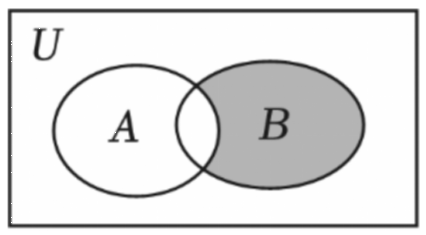
\includegraphics[width=0.26\textwidth]{figures/gao76_q14_venn.png}
\end{center}

\keepwithprev
A. $\{x\mid-2\leqslant x<4\}$\qquad B. $\{x\mid-1\leqslant x\leqslant3\}$

C. $\{x\mid x\leqslant3\text{ 或 }x\geqslant4\}$\qquad D. $\{x\mid-2\leqslant x\leqslant4\}$

\ifanswer
\solbegin
\step{全集 $U=\R$，集合 $A=\{x\mid x<-1\text{ 或 }x>4\}$，}
\step{$B=\{x\mid x^2-x-6\leqslant0\}=\{x\mid-2\leqslant x\leqslant3\}$，故 $A\cap B=\{x\mid-2\leqslant x<-1\}$，}
\step{故阴影部分表示的集合为 $\overline{A\cap B}=\{x\mid-1\leqslant x\leqslant3\}$. 故选 $B$.}
\solend
\fi

\item 设 $a$、$b$、$c\in\R$，给出下列命题：①若 $a>b$，则 $a^2>b^2$，②“$a>b$”是“$a^3>b^3$”的充要条件，③若 $a^2>b^2$，则 $|a|>|b|$，④若 $\dfrac ab>1$，则 $a>b$，⑤若 $a>b$，$c\neq0$，则 $\dfrac a{c^2}>\dfrac b{c^2}$，其中真命题的个数是\mbox{（\quad）}

\keepwithprev
A. $1$ 个\qquad B. $2$ 个\qquad C. $3$ 个\qquad D. $4$ 个

\ifanswer
\solbegin
\step{对于①，取 $a=2$，$b=-2$，满足 $a>b$，而 $a^2=b^2$，故为假命题；}
\step{对于②，$a>b\Leftrightarrow a^3-b^3=(a-b)(a^2+ab+b^2)=(a-b)\left[\left(a+\dfrac12b\right)^2+\dfrac34b^2\right]>0$}
\step{$\Leftrightarrow a^3>b^3$，故为真命题；}
\step{对于③，$a^2>b^2\Leftrightarrow|a|^2>|b|^2\Leftrightarrow|a|>|b|$，故为真命题；}
\step{对于④，取 $a=-2$，$b=-1$，满足 $\dfrac ab>1$，而 $a<b$，故为假命题；}
\step{对于⑤，由题意得 $c^2>0$，由 $a>b$，则 $\dfrac a{c^2}>\dfrac b{c^2}$，故为真命题.}
\step{故选 $C$.}
\solend
\fi

\item 已知关于 $x$ 的两个一元二次不等式 $a_1x^2+b_1x+c_1>0$，$a_2x^2+b_2x+c_2>0$ 的解集分别为 $A$、$B$，其中 $a_i$、$b_i$、$c_i(i=1,2)$ 为常数且不为零，则“$\dfrac{a_1}{a_2}=\dfrac{b_1}{b_2}=\dfrac{c_1}{c_2}$”是“$A=B$”\mbox{（\quad）}

\keepwithprev
A. 充分不必要条件\qquad B. 必要不充分条件

C. 充要条件\qquad D. 既不充分也不必要条件

\ifanswer
\solbegin
\step{设 $\dfrac{a_1}{a_2}=\dfrac{b_1}{b_2}=\dfrac{c_1}{c_2}=\lambda$，}
\step{①当 $\lambda>0$ 时，则 $a_1=\lambda a_2$，$b_1=\lambda b_2$，$c_1=\lambda c_2$，}
\step{$a_1x^2+b_1x+c_1>0\Leftrightarrow\lambda a_2x^2+\lambda b_2x+\lambda c_2>0\Leftrightarrow a_2x^2+b_2x+c_2>0$，}
\step{所以 $A=B$，}
\step{②当 $\lambda<0$ 时，则 $a_1=\lambda a_2$，$b_1=\lambda b_2$，$c_1=\lambda c_2$，}
\step{$a_1x^2+b_1x+c_1>0\Leftrightarrow\lambda a_2x^2+\lambda b_2x+\lambda c_2>0\Leftrightarrow a_2x^2+b_2x+c_2<0$，}
\step{所以 $A\neq B$，充分性不成立，}
\step{当 $A=B=\R$ 时，则 $\Delta<0$ 且 $a_1$、$a_2>0$，$\dfrac{a_1}{a_2}=\dfrac{b_1}{b_2}=\dfrac{c_1}{c_2}$ 不一定成立，}
\step{必要性不成立.}
\step{所以 $\dfrac{a_1}{a_2}=\dfrac{b_1}{b_2}=\dfrac{c_1}{c_2}$ 是 $A=B$ 的既不充分也不必要条件，故选 $D$.}
\solend
\fi

\end{enumerate}

\bigsec{三、解答题}

\begin{enumerate}
\setcounter{enumi}{16}

\item 求下列关于 $x$ 的不等式（组）的解集.

（1）$\begin{cases}9x^2-6x-24>0\\ \dfrac{x+3}{x-1}>2\end{cases}$；

（2）$|2x+1|-|2-x|>2$.

\ifanswer
\solbegin
\stepm{(1)}{不等式 $\dfrac{x+3}{x-1}>2$ 可化为 $\dfrac{x+3}{x-1}-2>0$，}
\step{即 $\dfrac{-x+5}{x-1}>0$，即 $(x-1)(x-5)<0$，解得 $1<x<5$，}
\step{不等式 $9x^2-6x-24>0$ 可化为 $(3x+4)(x-2)>0$，}
\step{解得 $x<-\dfrac43$ 或 $x>2$，}
\step{所以不等式的解集为 $(2,5)$.}
\stepm{(2)}{当 $x\leqslant-\dfrac12$ 时，$|2x+1|-|2-x|>2$ 等价于 $-2x-1-(2-x)>2$，}
\step{解得 $x<-5$，所以 $x<-5$，}
\step{当 $-\dfrac12<x<2$ 时，$|2x+1|-|2-x|>2$ 等价于 $2x+1-(2-x)>2$，}
\step{解得 $x>1$，所以 $1<x<2$，}
\step{当 $x\geqslant2$ 时，$|2x+1|-|2-x|>2$ 等价于 $2x+1-(x-2)>2$，}
\step{解得 $x>-1$，所以 $x\geqslant2$，}
\step{综上，$|2x+1|-|2-x|>2$ 的解集为 $(-\infty,-5)\cup(1,+\infty)$.}
\solend
\fi

\ansspace

\item 设 $m$ 为实数，求关于 $x$ 与 $y$ 的二元一次方程组 $\begin{cases}y=x+m\\ mx-y=4\end{cases}$ 的解集.

\ifanswer
\solbegin
\step{消去 $y$ 得 $(m-1)x=m+4$，}
\step{当 $m-1=0$，即 $m=1$ 时，$0=5$ 不成立，则 $x$ 无解，原方程组的解集为 $\varnothing$；}
\step{当 $m-1\neq0$，即 $m\neq1$ 时，则 $x=\dfrac{m+4}{m-1}$，$y=\dfrac{m+4}{m-1}+m=\dfrac{m^2+4}{m-1}$，}
\step{原方程组的解集为 $\left\{\left(\dfrac{m+4}{m-1},\dfrac{m^2+4}{m-1}\right)\right\}$.}
\step{综上所述，当 $m=1$ 时，方程组的解集为 $\varnothing$；}
\step{当 $m\neq1$ 时，方程组的解集为 $\left\{\left(\dfrac{m+4}{m-1},\dfrac{m^2+4}{m-1}\right)\right\}$.}
\solend
\fi

\ansspace

\item 已知集合 $A=\{x\mid-2\leqslant x-1\leqslant5\}$，集合 $B=\{x\mid m+1\leqslant x\leqslant2m-1\}(m\in\R)$.

（1）若 $m=4$，全集 $U=\R$，求 $A\cap B$；

（2）设命题 $p:x\in A$；命题 $q:x\in B$，若命题 $p$ 是命题 $q$ 的必要不充分条件，求实数 $m$ 的取值范围.

\ifanswer
\solbegin
\stepm{(1)}{由题意得 $A=\{x\mid-2\leqslant x-1\leqslant5\}=\{x\mid-1\leqslant x\leqslant6\}$，}
\step{当 $m=4$ 时，$B=\{x\mid5\leqslant x\leqslant7\}$，$A\cap B=\{x\mid5\leqslant x\leqslant6\}$；}
\stepm{(2)}{因为命题 $p$ 是命题 $q$ 的必要不充分条件，所以集合 $B$ 是集合 $A$ 的真子集，}
\step{当 $B=\varnothing$ 时，$m+1>2m-1$，解得 $m<2$，}
\step{当 $B\neq\varnothing$ 时，$\begin{cases}m+1\leqslant2m-1\\ m+1\geqslant-1\\ 2m-1\leqslant6\end{cases}$（等号不能同时成立），解得 $2\leqslant m\leqslant\dfrac72$，}
\step{综上所述，实数 $m$ 的取值范围为 $\left(-\infty,\dfrac72\right]$.}
\solend
\fi

\ansspace

\item （1）已知实数 $x\neq0$，求 $x+\dfrac1x$ 的取值范围；

（2）如图，要设计一张矩形海报，该海报含有大小相等的左右两个矩形栏目（即图中阴影部分），这两栏的面积之和为 $18000\,\mathrm{cm}^2$，四周空白的宽度为 $10\,\mathrm{cm}$，两栏之间的中缝空白的宽度为 $16\,\mathrm{cm}$，怎样确定海报的高与宽的尺寸（单位：$\mathrm{cm}$），能使矩形海报面积 $S$ 最小？最小面积是多少？

\begin{center}
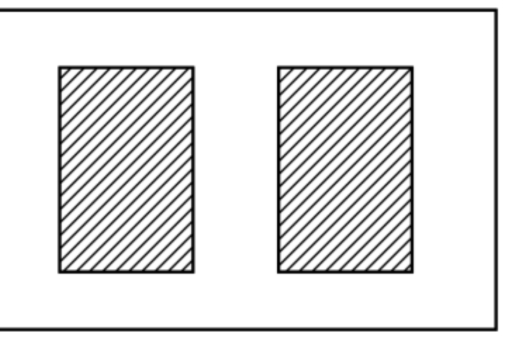
\includegraphics[width=0.34\textwidth]{figures/gao76_q20_poster.png}
\end{center}

\ifanswer
\solbegin
\stepm{(1)}{当 $x>0$ 时，$x+\dfrac1x\geqslant2\sqrt{x\times\dfrac1x}=2$，当且仅当 $x=\dfrac1x$，即 $x=1$ 取等号，}
\step{当 $x<0$ 时，$-x-\dfrac1x\geqslant2\sqrt{(-x)\times\dfrac1{-x}}=2$，所以 $x+\dfrac1x\leqslant-2$，}
\step{当且仅当 $-x=-\dfrac1x$，即 $x=-1$ 取等号，}
\step{综上所述，$x+\dfrac1x$ 的取值范围为 $(-\infty,-2]\cup[2,+\infty)$.}
\stepm{(2)}{设矩形栏目宽为 $x$，高为 $y$，则 $2xy=18000$，}
\step{所以 $S=(2x+36)(y+20)=2xy+36y+40x+720$}
% 原卷此行把 18720 写作 36720，照录（见文件头“原卷笔误/存疑”①）
\step{$=18000+36y+40x+720\geqslant18720+2\sqrt{36y\times40x}$}
\step{$=36720+2\sqrt{36\times40\times18000}=18720+7200=25920$，}
\step{当且仅当 $36y=40x$，即 $x=90$，$y=100$ 取等号，}
\step{所以海报的高为 $120\,\mathrm{cm}$ 与宽为 $216\,\mathrm{cm}$，可使矩形海报面积 $S$ 最小，}
\step{最小面积为 $25920$.}
\solend
\fi

\ansspace

\item 若实数 $x$、$y$、$m$ 满足 $|x-m|>|y-m|$，则称 $x$ 比 $y$ 远离 $m$.

（1）$0$ 比 $\dfrac12$ 远离 $2$ 吗？说明理由；

（2）若 $\dfrac1{2x-1}$ 比 $\dfrac12$ 远离 $1$，求实数 $x$ 的取值范围；

（3）若 $m\leqslant1$，$x+y=2$，试问：$x$ 与 $x^2+y^2$ 哪一个更远离 $m$，并说明理由.

\ifanswer
\solbegin
\stepm{(1)}{$0$ 比 $\dfrac12$ 远离 $2$，理由为：}
\step{由于 $|0-2|=2>\dfrac32=\left|\dfrac12-2\right|$，所以 $0$ 比 $\dfrac12$ 远离 $2$.}
\stepm{(2)}{由 $\dfrac1{2x-1}$ 比 $\dfrac12$ 远离 $1$，得 $\left|\dfrac1{2x-1}-1\right|>\left|\dfrac12-1\right|$，即 $\left|\dfrac1{2x-1}-1\right|>\dfrac12$，}
\step{则 $\dfrac1{2x-1}-1>\dfrac12$ 或 $\dfrac1{2x-1}-1<-\dfrac12$，整理得 $\dfrac1{2x-1}>\dfrac32$ 或 $\dfrac1{2x-1}<\dfrac12$，}
\step{因此 $0<2x-1<\dfrac23$ 或 $2x-1<0$ 或 $2x-1>2$，}
\step{解得 $\dfrac12<x<\dfrac56$ 或 $x<\dfrac12$ 或 $x>\dfrac32$，}
\step{所以 $x$ 的取值范围是 $\left(-\infty,\dfrac12\right)\cup\left(\dfrac12,\dfrac56\right)\cup\left(\dfrac32,+\infty\right)$.}
\stepm{(3)}{$x^2+y^2$ 比 $x$ 更远离 $m$，理由为：}
\step{由 $x^2+y^2\geqslant\dfrac{(x+y)^2}2=2\geqslant m$，得 $|x^2+y^2-m|=x^2+y^2-m$，}
\step{由 $x+y=2$，得 $x^2+y^2=x^2+(2-x)^2=2x^2-4x+4$，}
\step{于是 $|x^2+y^2-m|-|x-m|=2x^2-4x+4-m-|x-m|$，}
\step{当 $x\geqslant m$ 时，$|x^2+y^2-m|-|x-m|=2x^2-4x+4-m-(x-m)$}
\step{$=2\left(x-\dfrac54\right)^2+\dfrac78>0$，即 $|x^2+y^2-m|>|x-m|$；}
\step{当 $x<m$ 时，$|x^2+y^2-m|-|x-m|=2x^2-4x+4-m+(x-m)$}
\step{$=2\left(x-\dfrac34\right)^2+\dfrac{23}8-2m$，}
\step{由 $m\leqslant1$，得 $\dfrac{23}8-2m>0$，因此 $2\left(x-\dfrac34\right)^2+\dfrac{23}8-2m>0$，}
\step{即 $|x^2+y^2-m|>|x-m|$，}
\step{所以 $|x^2+y^2-m|>|x-m|$，即 $x^2+y^2$ 比 $x$ 更远离 $m$.}
\solend
\fi

\ansspace*[7]

\end{enumerate}

\end{document}
"
% 紧凑版：xelatex "\def\iscompact{1}% 高一76_六十中学_10月月考.tex
%   —— 高一上数学“2026-2027 年六十中学高一上 10 月月考”（讲评版）
% 试卷版：xelatex 高一76_六十中学_10月月考.tex
% 答案版：xelatex "\def\isanswer{1}\input{高一76_六十中学_10月月考.tex}"
% 紧凑版：xelatex "\def\iscompact{1}\input{高一76_六十中学_10月月考.tex}"
%
% 原始材料：微信公众号“魔都数学加油站”文章，连载“27学年高一76”；
% 原文标题“27学年高一76——2026-2027年上海市六十中学高一上10月月考”；
% 原文链接：https://mp.weixin.qq.com/s/GrKZjQrV1Xb0wy0BUuzAHw。
% 页面标注发布时间 2026-10-22 21:45（上海）。
% 正文为 10 张 PNG 页（`原图/高一76_六十中学_10月月考/01..10.png`）：
% 第 4、5、8、9 页为 4762×6735，其余 6 页为 2560×3620，均按页序读取。
% 10 页全为试卷正文页（卷首标题在第 1 页页顶，卷末第 21 题 (3) 解析止于第 10 页），
% 无封面页、目录页、二维码或宣传页。粉色斜排“魔都数学加油站”为卷面水印，未录入。
%
% 卷首标题：照卷面印作“2026-2027 年六十中学高一上 10 月月考”（黑体加粗一行）。
% 原卷年份区间用半角连字符，本稿按全稿惯例排 en dash；原卷无副标题。
%
% 篇幅与题号：原卷自第 3 题起编号（第 1、2 题不在本卷内）。填空题 3—12（10 题）、
% 选择题 13—16（4 题）、解答题 17—21（5 题），共 19 题。本稿沿用原节与原题号，
% 只改排为全稿统一的大节样式。
%
% 讲评版：原卷第 3、5 题只印【答案】（“$(0,1)$”“$a$、$b$ 都不能被 $3$ 整除”），
% 本稿只给 \ans{}；其余 17 题均印【解析】，用 \solbegin…\solend。四道选择题的作答
% 括号原卷即留空，答案写在解析末句“故选 C／B／C／D”，照录在解析内，不另提 \ans{}。
%
% 副标题：原卷未印副标题。本稿按“知识模块”口径标作“集合与常用逻辑用语、不等式”：
% 19 题中集合与常用逻辑用语 6 题（第 5、12、14、16、19 题及第 4 题的恒等变形），
% 不等式 13 题（第 3、6—11、13、15、17、18、20、21 题），两类均确有分量，故并标。
% 口径同 高一63、高一68—75。
%
% 与原卷的排版差异：
%   ① 原卷每题下直接印【答案】/【解析】，本稿按全稿惯例将答案与解析置于答案版；
%   ② 原卷未印副标题，本稿按“知识模块”口径补出；
%   ③ 原卷填空横线约四个字宽，本稿按全稿惯例统一排 \blankline[4.4em]；
%   ④ 原卷数集记号排斜体 $R$、$N$（第 4、6、7、8、11、12、14、15、19、20 题），本稿
%      按全稿惯例改用 $\R$、$\N$（同 高一68—75）；第 7、19、20 题的“解集为 $\R$”同此；
%   ⑤ 原卷句末标点多为西文句点，均逐处照录；
%   ⑥ 第 17—21 题的子问原卷印作“（1）…（2）…”，本稿按 高一69—75 成例用行内
%      “（1）（2）（3）”段，解析中的子问标号用 \stepm{(1)}{…}；
%   ⑦ 每道解答题原卷未留作答空白，本稿按全稿惯例加 \ansspace（末题用 \ansspace*）；
%   ⑧ 选择题的作答括号原卷排半角“(    )”，本稿按全稿惯例排 \mbox{（\quad）}；
%      选项行排照原卷——第 13、14、15、16 题一行两条、分两行排（本稿按原卷分行）；
%   ⑨ 第 10、11、17—21 题解析中的不等式组／方程组，原卷均排作“{”连接的多行式，
%      本稿按全稿惯例排 cases；
%   ⑩ 第 14 题题干右侧有一幅韦恩图（全集矩形内含 A、B 两圆，B 涂灰）：本稿按原卷
%      截图裁取（`figures/gao76_q14_venn.png`，由第 5 页原图裁出、去除粉色水印后转
%      灰度，未放大），放在题干之后、选项之前，仅答案版出；
%   ⑪ 第 20 题 (2) 题干右侧有一幅示意图（大矩形内两个斜线阴影小矩形）：本稿按原卷
%      截图裁取（`figures/gao76_q20_poster.png`，由第 8 页原图裁出、去除粉色水印后转
%      灰度，未放大），放在该小题文字之后，仅答案版出。
%
% 原卷笔误/存疑（均照录未改，正文对应处另有 % 注）：
%   ① 第 20 题 (2) 解析第 3 行把 $2xy+720$ 写成 $36720$（实为 $18000+720=18720$），
%      同式下一行又写回 $18720$，前后不一致；原卷如此，照录未改。
%   ② 第 14 题的韦恩图阴影是把整个 $B$ 圆（含 $A\cap B$ 部分）涂灰，而解析按
%      $\overline{A\cap B}$ 求解，二者不一致；原卷图文如此，照录未改。
%
% 行数核对：逐题数 \step/\stepm 条数与原卷【解析】印刷行数，17 题逐一相符，
% 合计 118 条 / 118 行（Q4：3；Q6：4；Q7：1；Q8：6；Q9：3；Q10：7；Q11：4；
% Q12：16；Q13：1；Q14：3；Q15：7；Q16：10；Q17：12；Q18：6；Q19：6；Q20：11；
% Q21：18）。另第 3、5 题只印【答案】，各提 \ans{}，不计入 \step 账。
%
% 插图：第 14 题题干的韦恩图、第 20 题 (2) 的示意图，见上⑩⑪；其余题干无配图。
%
\documentclass[a4paper,11pt]{article}
\usepackage{common}

\begin{document}

\examtitlest[3]{2026--2027 年六十中学高一上 10 月月考}{集合与常用逻辑用语、不等式}

\bigsec{一、填空题}

\begin{enumerate}
\setcounter{enumi}{2}

\item 不等式 $\dfrac{x}{1-x}>0$ 的解集是\blankline[4.4em].

\ifanswer
\ans{$(0,1)$}
\fi

\item 已知 $2x^2+x+1=a(x+1)^2+b(x+1)+2$，对 $x\in\R$ 恒成立，$ab=$\blankline[4.4em].

\ifanswer
\solbegin
\step{若 $2x^2+x+1=a(x+1)^2+b(x+1)+2$ 对 $x\in\R$ 恒成立，}
\step{即 $2x^2+x+1=ax^2+(2a+b)x+a+b+2$ 对 $x\in\R$ 恒成立，}
\step{必有 $\begin{cases}a=2\\ 2a+b=1\\ a+b+2=1\end{cases}$，解得 $a=2$，$b=-3$，所以 $ab=-6$.}
\solend
\fi

\item 利用反证法证明命题：“如果 $a$、$b\in\N$，$ab$ 可被 $3$ 整除，那么 $a$、$b$ 中至少有一个能被 $3$ 整除”时，假设的内容应是\blankline[4.4em].

\ifanswer
\ans{$a$、$b$ 都不能被 $3$ 整除}
\fi

\item 已知 $x\in\R$，方程 $|x+1|+|2-x|=3$ 的解集为\blankline[4.4em].

\ifanswer
\solbegin
\step{当 $x<-1$ 时，则 $|x+1|+|2-x|=-x-1+2-x=1-2x>3$；}
\step{当 $-1\leqslant x\leqslant2$ 时，则 $|x+1|+|2-x|=x+1+2-x=3$；}
\step{当 $x>2$ 时，则 $|x+1|+|2-x|=x+1+x-2=2x-1>3$.}
\step{综上所述，原方程的解集为 $[-1,2]$.}
\solend
\fi

\item 若关于 $x$ 的不等式 $x^2+kx+1\geqslant0$ 的解集为 $\R$，则实数 $k$ 的取值范围是\blankline[4.4em].

\ifanswer
\solbegin
\step{$\Delta=k^2-4\leqslant0\Rightarrow-2\leqslant k\leqslant2$，所以实数 $k$ 的取值范围是 $[-2,2]$.}
\solend
\fi

\item 已知 $a$、$b\in\R$，且 $ab>0$，则下列不等式中，恒成立的序号是\blankline[4.4em].

① $a^2+b^2>2ab$；② $a+b\geqslant2\sqrt{ab}$；③ $\dfrac1a+\dfrac1b>\dfrac2{\sqrt{ab}}$；④ $\dfrac ba+\dfrac ab\geqslant2$.

\ifanswer
\solbegin
\step{因为 $a^2+b^2\geqslant2ab$ 对于 $a$、$b\in\R$ 恒成立，当且仅当 $a=b$ 时取等号，}
\step{所以①错误；}
\step{对于②，③，显然 $a<0$，$b<0$ 时，不等式均不成立，即②和③错误；}
\step{对于④，因为 $ab>0$，所以 $\dfrac ba>0,\dfrac ab>0$，}
\step{由基本不等式得 $\dfrac ba+\dfrac ab\geqslant2\sqrt{\dfrac ba\cdot\dfrac ab}=2$，即④正确.}
\step{故正确的是④.}
\solend
\fi

\item 已知正实数 $m$、$n$ 满足 $m+\dfrac2n=1$，则 $\dfrac1m+2n$ 的最小值为\blankline[4.4em].

\ifanswer
\solbegin
\step{$\dfrac1m+2n=\left(m+\dfrac2n\right)\left(\dfrac1m+2n\right)=5+2mn+\dfrac2{mn}$，}
\step{因为 $mn>0$，所以 $2mn+\dfrac2{mn}\geqslant2\sqrt{2mn\cdot\dfrac2{mn}}=4$，}
\step{当且仅当 $2mn=\dfrac2{mn}$，即 $m=\dfrac13$，$n=3$ 时取等号，所以 $\dfrac1m+2n$ 的最小值为 $9$.}
\solend
\fi

\item 若关于 $x$ 的不等式组 $\begin{cases}3x+1>0\\ x+\dfrac1a\leqslant2\end{cases}$ 恰好有两个整数解，则实数 $a$ 的取值范围为\blankline[4.4em].

\ifanswer
\solbegin
\step{由 $3x+1>0$ 得 $x>-\dfrac13$；若 $a<0$，则 $\dfrac1a<0$，由 $x+\dfrac1a\leqslant2$ 得 $x\leqslant2-\dfrac1a>2$，}
\step{则解集 $\left(-\dfrac13,2-\dfrac1a\right]$ 必同时含有整数 $0$、$1$、$2$，不合题意；}
\step{又 $a=0$ 使 $\dfrac1a$ 无意义，故 $a>0$；}
\step{此时原不等式组的解集为 $\left(-\dfrac13,2-\dfrac1a\right]$，}
\step{其中大于 $-\dfrac13$ 的整数依次为 $0$，$1$，$2$，$\cdots$，}
\step{恰有两个整数解即解集只含 $0$ 与 $1$，故 $1\leqslant2-\dfrac1a<2$，即 $\dfrac1a\leqslant1$ 且 $\dfrac1a>0$，}
\step{结合 $a>0$，解得 $a\geqslant1$.}
\solend
\fi

\item 已知 $a\in\R$，若关于 $x$ 的方程 $x^2+ax+a^2-8=0$ 有两个实根 $x_1$、$x_2$，且 $\dfrac1{x_1}+\dfrac1{x_2}=-\dfrac12$，则 $a$ 的值为\blankline[4.4em].

\ifanswer
\solbegin
\step{由题意得 $\Delta=a^2-4(a^2-8)=32-3a^2\geqslant0$，解得 $a^2\leqslant\dfrac{32}3$，}
\step{由韦达定理得 $x_1+x_2=-a$，$x_1x_2=a^2-8$，}
\step{则 $\dfrac1{x_1}+\dfrac1{x_2}=\dfrac{x_1+x_2}{x_1x_2}=\dfrac{-a}{a^2-8}=-\dfrac12$，即 $a^2-2a-8=(a-4)(a+2)=0$，}
\step{解得 $a=4$ 或 $a=-2$，又 $a^2\leqslant\dfrac{32}3$，则 $a=-2$.}
\solend
\fi

\item 已知有限集 $A=\{a_1,a_2,\cdots,a_n\}(n\geqslant2,n\in\N)$，若 $A$ 中元素 $a_i(i=1,2,\cdots,n)$ 满足 $a_1+a_2+\cdots+a_n=a_1\times a_2\times\cdots\times a_n$，就称 $A$ 为“完美集”，以下四个命题：

①集合 $\{-1-\sqrt3,-1+\sqrt3\}$ 不是“完美集”；

②若 $a_1$、$a_2$ 是两个不同的正数，且 $\{a_1,a_2\}$ 是“完美集”，则 $a_1$、$a_2$ 至少有一个大于 $2$；

③二元“完美集”有无穷多个；

④若 $a_i$ 均为正整数，则“完美集”$A$ 有且只有一个，且 $n=3$.

其中，真命题的序号是\blankline[4.4em].

\ifanswer
\solbegin
\step{对于①选项：$(-1-\sqrt3)+(-1+\sqrt3)=-2$，$(-1-\sqrt3)\times(-1+\sqrt3)=-2$，}
\step{故 $(-1-\sqrt3)+(-1+\sqrt3)=(-1-\sqrt3)\times(-1+\sqrt3)$，}
\step{所以集合 $\{-1-\sqrt3,-1+\sqrt3\}$ 是“完美集”，故①错误；}
\step{对于②选项：集合 $\{a_1,a_2\}$ 是“完美集”，设 $a_1+a_2=a_1a_2=t>0$，}
\step{则 $a_1$、$a_2$ 可以看成一元二次方程 $x^2-tx+t=0$ 的两正根，则 $\Delta=t^2-4t>0$，}
\step{解得 $t<0$（舍）或 $t>4$，即 $a_1a_2>4$，所以至少有一个大于 $2$，故②正确；}
\step{对于③选项：由②得一元二次方程 $x^2-tx+t=0$ 当 $t$ 取不同值时，}
\step{$a_1$、$a_2$ 的值是不同的，因而二元“完美集”有无穷多个，故③正确；}
\step{对于④选项：设 $a_1<a_2<a_3<\cdots<a_n$，}
\step{则 $a_1\times a_2\times\cdots\times a_n=a_1+a_2+\cdots+a_n<na_n$，}
\step{所以 $a_1\times a_2\times\cdots\times a_{n-1}<n$，又 $a_i\in\N^*$，所以 $n\leqslant3$，}
\step{当 $n=2$ 时，$a_1<2$，则 $a_1=1$，$a_1a_2\neq a_1+a_2$，不合题意，}
\step{当 $n=3$ 时，$a_1a_2<3$，所以只能是 $a_1=1$，$a_2=2$，}
\step{由 $a_1+a_2+a_3=a_1a_2a_3$，代入解得 $a_3=3$，所以此时“完美集”只有一个，}
\step{为 $\{1,2,3\}$，故④正确.}
\step{故正确的是②③④.}
\solend
\fi

\end{enumerate}

\bigsec{二、选择题}

\begin{enumerate}
\setcounter{enumi}{12}

\item 已知 $x$、$y\in\R$，则“$xy\geqslant0$”是“$xy=|xy|$”的\mbox{（\quad）}

\keepwithprev
A. 充分非必要条件\qquad B. 必要非充分条件

C. 充要条件\qquad D. 既非充分也非必要条件

\ifanswer
\solbegin
\step{$xy\geqslant0\Leftrightarrow xy=|xy|$，故“$xy\geqslant0$”是“$xy=|xy|$”的充要条件. 故选 $C$.}
\solend
\fi

\needvspace{22\baselineskip}
\item 已知全集 $U=\R$，集合 $A=\{x\mid x<-1\text{ 或 }x>4\}$，$B=\{x\mid x^2-x-6\leqslant0\}$，则阴影部分表示的集合为\mbox{（\quad）}

\begin{center}
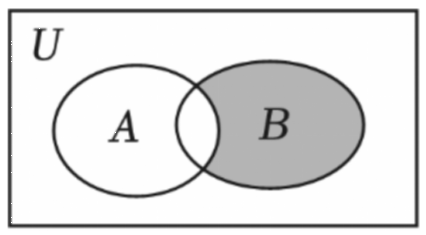
\includegraphics[width=0.26\textwidth]{figures/gao76_q14_venn.png}
\end{center}

\keepwithprev
A. $\{x\mid-2\leqslant x<4\}$\qquad B. $\{x\mid-1\leqslant x\leqslant3\}$

C. $\{x\mid x\leqslant3\text{ 或 }x\geqslant4\}$\qquad D. $\{x\mid-2\leqslant x\leqslant4\}$

\ifanswer
\solbegin
\step{全集 $U=\R$，集合 $A=\{x\mid x<-1\text{ 或 }x>4\}$，}
\step{$B=\{x\mid x^2-x-6\leqslant0\}=\{x\mid-2\leqslant x\leqslant3\}$，故 $A\cap B=\{x\mid-2\leqslant x<-1\}$，}
\step{故阴影部分表示的集合为 $\overline{A\cap B}=\{x\mid-1\leqslant x\leqslant3\}$. 故选 $B$.}
\solend
\fi

\item 设 $a$、$b$、$c\in\R$，给出下列命题：①若 $a>b$，则 $a^2>b^2$，②“$a>b$”是“$a^3>b^3$”的充要条件，③若 $a^2>b^2$，则 $|a|>|b|$，④若 $\dfrac ab>1$，则 $a>b$，⑤若 $a>b$，$c\neq0$，则 $\dfrac a{c^2}>\dfrac b{c^2}$，其中真命题的个数是\mbox{（\quad）}

\keepwithprev
A. $1$ 个\qquad B. $2$ 个\qquad C. $3$ 个\qquad D. $4$ 个

\ifanswer
\solbegin
\step{对于①，取 $a=2$，$b=-2$，满足 $a>b$，而 $a^2=b^2$，故为假命题；}
\step{对于②，$a>b\Leftrightarrow a^3-b^3=(a-b)(a^2+ab+b^2)=(a-b)\left[\left(a+\dfrac12b\right)^2+\dfrac34b^2\right]>0$}
\step{$\Leftrightarrow a^3>b^3$，故为真命题；}
\step{对于③，$a^2>b^2\Leftrightarrow|a|^2>|b|^2\Leftrightarrow|a|>|b|$，故为真命题；}
\step{对于④，取 $a=-2$，$b=-1$，满足 $\dfrac ab>1$，而 $a<b$，故为假命题；}
\step{对于⑤，由题意得 $c^2>0$，由 $a>b$，则 $\dfrac a{c^2}>\dfrac b{c^2}$，故为真命题.}
\step{故选 $C$.}
\solend
\fi

\item 已知关于 $x$ 的两个一元二次不等式 $a_1x^2+b_1x+c_1>0$，$a_2x^2+b_2x+c_2>0$ 的解集分别为 $A$、$B$，其中 $a_i$、$b_i$、$c_i(i=1,2)$ 为常数且不为零，则“$\dfrac{a_1}{a_2}=\dfrac{b_1}{b_2}=\dfrac{c_1}{c_2}$”是“$A=B$”\mbox{（\quad）}

\keepwithprev
A. 充分不必要条件\qquad B. 必要不充分条件

C. 充要条件\qquad D. 既不充分也不必要条件

\ifanswer
\solbegin
\step{设 $\dfrac{a_1}{a_2}=\dfrac{b_1}{b_2}=\dfrac{c_1}{c_2}=\lambda$，}
\step{①当 $\lambda>0$ 时，则 $a_1=\lambda a_2$，$b_1=\lambda b_2$，$c_1=\lambda c_2$，}
\step{$a_1x^2+b_1x+c_1>0\Leftrightarrow\lambda a_2x^2+\lambda b_2x+\lambda c_2>0\Leftrightarrow a_2x^2+b_2x+c_2>0$，}
\step{所以 $A=B$，}
\step{②当 $\lambda<0$ 时，则 $a_1=\lambda a_2$，$b_1=\lambda b_2$，$c_1=\lambda c_2$，}
\step{$a_1x^2+b_1x+c_1>0\Leftrightarrow\lambda a_2x^2+\lambda b_2x+\lambda c_2>0\Leftrightarrow a_2x^2+b_2x+c_2<0$，}
\step{所以 $A\neq B$，充分性不成立，}
\step{当 $A=B=\R$ 时，则 $\Delta<0$ 且 $a_1$、$a_2>0$，$\dfrac{a_1}{a_2}=\dfrac{b_1}{b_2}=\dfrac{c_1}{c_2}$ 不一定成立，}
\step{必要性不成立.}
\step{所以 $\dfrac{a_1}{a_2}=\dfrac{b_1}{b_2}=\dfrac{c_1}{c_2}$ 是 $A=B$ 的既不充分也不必要条件，故选 $D$.}
\solend
\fi

\end{enumerate}

\bigsec{三、解答题}

\begin{enumerate}
\setcounter{enumi}{16}

\item 求下列关于 $x$ 的不等式（组）的解集.

（1）$\begin{cases}9x^2-6x-24>0\\ \dfrac{x+3}{x-1}>2\end{cases}$；

（2）$|2x+1|-|2-x|>2$.

\ifanswer
\solbegin
\stepm{(1)}{不等式 $\dfrac{x+3}{x-1}>2$ 可化为 $\dfrac{x+3}{x-1}-2>0$，}
\step{即 $\dfrac{-x+5}{x-1}>0$，即 $(x-1)(x-5)<0$，解得 $1<x<5$，}
\step{不等式 $9x^2-6x-24>0$ 可化为 $(3x+4)(x-2)>0$，}
\step{解得 $x<-\dfrac43$ 或 $x>2$，}
\step{所以不等式的解集为 $(2,5)$.}
\stepm{(2)}{当 $x\leqslant-\dfrac12$ 时，$|2x+1|-|2-x|>2$ 等价于 $-2x-1-(2-x)>2$，}
\step{解得 $x<-5$，所以 $x<-5$，}
\step{当 $-\dfrac12<x<2$ 时，$|2x+1|-|2-x|>2$ 等价于 $2x+1-(2-x)>2$，}
\step{解得 $x>1$，所以 $1<x<2$，}
\step{当 $x\geqslant2$ 时，$|2x+1|-|2-x|>2$ 等价于 $2x+1-(x-2)>2$，}
\step{解得 $x>-1$，所以 $x\geqslant2$，}
\step{综上，$|2x+1|-|2-x|>2$ 的解集为 $(-\infty,-5)\cup(1,+\infty)$.}
\solend
\fi

\ansspace

\item 设 $m$ 为实数，求关于 $x$ 与 $y$ 的二元一次方程组 $\begin{cases}y=x+m\\ mx-y=4\end{cases}$ 的解集.

\ifanswer
\solbegin
\step{消去 $y$ 得 $(m-1)x=m+4$，}
\step{当 $m-1=0$，即 $m=1$ 时，$0=5$ 不成立，则 $x$ 无解，原方程组的解集为 $\varnothing$；}
\step{当 $m-1\neq0$，即 $m\neq1$ 时，则 $x=\dfrac{m+4}{m-1}$，$y=\dfrac{m+4}{m-1}+m=\dfrac{m^2+4}{m-1}$，}
\step{原方程组的解集为 $\left\{\left(\dfrac{m+4}{m-1},\dfrac{m^2+4}{m-1}\right)\right\}$.}
\step{综上所述，当 $m=1$ 时，方程组的解集为 $\varnothing$；}
\step{当 $m\neq1$ 时，方程组的解集为 $\left\{\left(\dfrac{m+4}{m-1},\dfrac{m^2+4}{m-1}\right)\right\}$.}
\solend
\fi

\ansspace

\item 已知集合 $A=\{x\mid-2\leqslant x-1\leqslant5\}$，集合 $B=\{x\mid m+1\leqslant x\leqslant2m-1\}(m\in\R)$.

（1）若 $m=4$，全集 $U=\R$，求 $A\cap B$；

（2）设命题 $p:x\in A$；命题 $q:x\in B$，若命题 $p$ 是命题 $q$ 的必要不充分条件，求实数 $m$ 的取值范围.

\ifanswer
\solbegin
\stepm{(1)}{由题意得 $A=\{x\mid-2\leqslant x-1\leqslant5\}=\{x\mid-1\leqslant x\leqslant6\}$，}
\step{当 $m=4$ 时，$B=\{x\mid5\leqslant x\leqslant7\}$，$A\cap B=\{x\mid5\leqslant x\leqslant6\}$；}
\stepm{(2)}{因为命题 $p$ 是命题 $q$ 的必要不充分条件，所以集合 $B$ 是集合 $A$ 的真子集，}
\step{当 $B=\varnothing$ 时，$m+1>2m-1$，解得 $m<2$，}
\step{当 $B\neq\varnothing$ 时，$\begin{cases}m+1\leqslant2m-1\\ m+1\geqslant-1\\ 2m-1\leqslant6\end{cases}$（等号不能同时成立），解得 $2\leqslant m\leqslant\dfrac72$，}
\step{综上所述，实数 $m$ 的取值范围为 $\left(-\infty,\dfrac72\right]$.}
\solend
\fi

\ansspace

\item （1）已知实数 $x\neq0$，求 $x+\dfrac1x$ 的取值范围；

（2）如图，要设计一张矩形海报，该海报含有大小相等的左右两个矩形栏目（即图中阴影部分），这两栏的面积之和为 $18000\,\mathrm{cm}^2$，四周空白的宽度为 $10\,\mathrm{cm}$，两栏之间的中缝空白的宽度为 $16\,\mathrm{cm}$，怎样确定海报的高与宽的尺寸（单位：$\mathrm{cm}$），能使矩形海报面积 $S$ 最小？最小面积是多少？

\begin{center}
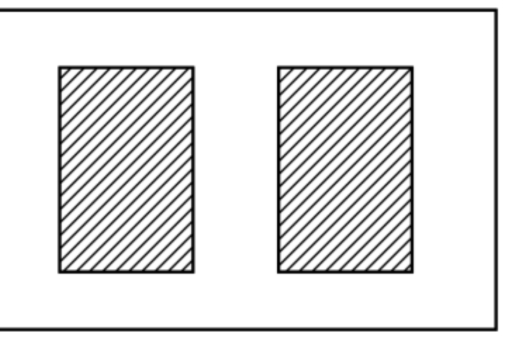
\includegraphics[width=0.34\textwidth]{figures/gao76_q20_poster.png}
\end{center}

\ifanswer
\solbegin
\stepm{(1)}{当 $x>0$ 时，$x+\dfrac1x\geqslant2\sqrt{x\times\dfrac1x}=2$，当且仅当 $x=\dfrac1x$，即 $x=1$ 取等号，}
\step{当 $x<0$ 时，$-x-\dfrac1x\geqslant2\sqrt{(-x)\times\dfrac1{-x}}=2$，所以 $x+\dfrac1x\leqslant-2$，}
\step{当且仅当 $-x=-\dfrac1x$，即 $x=-1$ 取等号，}
\step{综上所述，$x+\dfrac1x$ 的取值范围为 $(-\infty,-2]\cup[2,+\infty)$.}
\stepm{(2)}{设矩形栏目宽为 $x$，高为 $y$，则 $2xy=18000$，}
\step{所以 $S=(2x+36)(y+20)=2xy+36y+40x+720$}
% 原卷此行把 18720 写作 36720，照录（见文件头“原卷笔误/存疑”①）
\step{$=18000+36y+40x+720\geqslant18720+2\sqrt{36y\times40x}$}
\step{$=36720+2\sqrt{36\times40\times18000}=18720+7200=25920$，}
\step{当且仅当 $36y=40x$，即 $x=90$，$y=100$ 取等号，}
\step{所以海报的高为 $120\,\mathrm{cm}$ 与宽为 $216\,\mathrm{cm}$，可使矩形海报面积 $S$ 最小，}
\step{最小面积为 $25920$.}
\solend
\fi

\ansspace

\item 若实数 $x$、$y$、$m$ 满足 $|x-m|>|y-m|$，则称 $x$ 比 $y$ 远离 $m$.

（1）$0$ 比 $\dfrac12$ 远离 $2$ 吗？说明理由；

（2）若 $\dfrac1{2x-1}$ 比 $\dfrac12$ 远离 $1$，求实数 $x$ 的取值范围；

（3）若 $m\leqslant1$，$x+y=2$，试问：$x$ 与 $x^2+y^2$ 哪一个更远离 $m$，并说明理由.

\ifanswer
\solbegin
\stepm{(1)}{$0$ 比 $\dfrac12$ 远离 $2$，理由为：}
\step{由于 $|0-2|=2>\dfrac32=\left|\dfrac12-2\right|$，所以 $0$ 比 $\dfrac12$ 远离 $2$.}
\stepm{(2)}{由 $\dfrac1{2x-1}$ 比 $\dfrac12$ 远离 $1$，得 $\left|\dfrac1{2x-1}-1\right|>\left|\dfrac12-1\right|$，即 $\left|\dfrac1{2x-1}-1\right|>\dfrac12$，}
\step{则 $\dfrac1{2x-1}-1>\dfrac12$ 或 $\dfrac1{2x-1}-1<-\dfrac12$，整理得 $\dfrac1{2x-1}>\dfrac32$ 或 $\dfrac1{2x-1}<\dfrac12$，}
\step{因此 $0<2x-1<\dfrac23$ 或 $2x-1<0$ 或 $2x-1>2$，}
\step{解得 $\dfrac12<x<\dfrac56$ 或 $x<\dfrac12$ 或 $x>\dfrac32$，}
\step{所以 $x$ 的取值范围是 $\left(-\infty,\dfrac12\right)\cup\left(\dfrac12,\dfrac56\right)\cup\left(\dfrac32,+\infty\right)$.}
\stepm{(3)}{$x^2+y^2$ 比 $x$ 更远离 $m$，理由为：}
\step{由 $x^2+y^2\geqslant\dfrac{(x+y)^2}2=2\geqslant m$，得 $|x^2+y^2-m|=x^2+y^2-m$，}
\step{由 $x+y=2$，得 $x^2+y^2=x^2+(2-x)^2=2x^2-4x+4$，}
\step{于是 $|x^2+y^2-m|-|x-m|=2x^2-4x+4-m-|x-m|$，}
\step{当 $x\geqslant m$ 时，$|x^2+y^2-m|-|x-m|=2x^2-4x+4-m-(x-m)$}
\step{$=2\left(x-\dfrac54\right)^2+\dfrac78>0$，即 $|x^2+y^2-m|>|x-m|$；}
\step{当 $x<m$ 时，$|x^2+y^2-m|-|x-m|=2x^2-4x+4-m+(x-m)$}
\step{$=2\left(x-\dfrac34\right)^2+\dfrac{23}8-2m$，}
\step{由 $m\leqslant1$，得 $\dfrac{23}8-2m>0$，因此 $2\left(x-\dfrac34\right)^2+\dfrac{23}8-2m>0$，}
\step{即 $|x^2+y^2-m|>|x-m|$，}
\step{所以 $|x^2+y^2-m|>|x-m|$，即 $x^2+y^2$ 比 $x$ 更远离 $m$.}
\solend
\fi

\ansspace*[7]

\end{enumerate}

\end{document}
"
%
% 原始材料：微信公众号“魔都数学加油站”文章，连载“27学年高一76”；
% 原文标题“27学年高一76——2026-2027年上海市六十中学高一上10月月考”；
% 原文链接：https://mp.weixin.qq.com/s/GrKZjQrV1Xb0wy0BUuzAHw。
% 页面标注发布时间 2026-10-22 21:45（上海）。
% 正文为 10 张 PNG 页（`原图/高一76_六十中学_10月月考/01..10.png`）：
% 第 4、5、8、9 页为 4762×6735，其余 6 页为 2560×3620，均按页序读取。
% 10 页全为试卷正文页（卷首标题在第 1 页页顶，卷末第 21 题 (3) 解析止于第 10 页），
% 无封面页、目录页、二维码或宣传页。粉色斜排“魔都数学加油站”为卷面水印，未录入。
%
% 卷首标题：照卷面印作“2026-2027 年六十中学高一上 10 月月考”（黑体加粗一行）。
% 原卷年份区间用半角连字符，本稿按全稿惯例排 en dash；原卷无副标题。
%
% 篇幅与题号：原卷自第 3 题起编号（第 1、2 题不在本卷内）。填空题 3—12（10 题）、
% 选择题 13—16（4 题）、解答题 17—21（5 题），共 19 题。本稿沿用原节与原题号，
% 只改排为全稿统一的大节样式。
%
% 讲评版：原卷第 3、5 题只印【答案】（“$(0,1)$”“$a$、$b$ 都不能被 $3$ 整除”），
% 本稿只给 \ans{}；其余 17 题均印【解析】，用 \solbegin…\solend。四道选择题的作答
% 括号原卷即留空，答案写在解析末句“故选 C／B／C／D”，照录在解析内，不另提 \ans{}。
%
% 副标题：原卷未印副标题。本稿按“知识模块”口径标作“集合与常用逻辑用语、不等式”：
% 19 题中集合与常用逻辑用语 6 题（第 5、12、14、16、19 题及第 4 题的恒等变形），
% 不等式 13 题（第 3、6—11、13、15、17、18、20、21 题），两类均确有分量，故并标。
% 口径同 高一63、高一68—75。
%
% 与原卷的排版差异：
%   ① 原卷每题下直接印【答案】/【解析】，本稿按全稿惯例将答案与解析置于答案版；
%   ② 原卷未印副标题，本稿按“知识模块”口径补出；
%   ③ 原卷填空横线约四个字宽，本稿按全稿惯例统一排 \blankline[4.4em]；
%   ④ 原卷数集记号排斜体 $R$、$N$（第 4、6、7、8、11、12、14、15、19、20 题），本稿
%      按全稿惯例改用 $\R$、$\N$（同 高一68—75）；第 7、19、20 题的“解集为 $\R$”同此；
%   ⑤ 原卷句末标点多为西文句点，均逐处照录；
%   ⑥ 第 17—21 题的子问原卷印作“（1）…（2）…”，本稿按 高一69—75 成例用行内
%      “（1）（2）（3）”段，解析中的子问标号用 \stepm{(1)}{…}；
%   ⑦ 每道解答题原卷未留作答空白，本稿按全稿惯例加 \ansspace（末题用 \ansspace*）；
%   ⑧ 选择题的作答括号原卷排半角“(    )”，本稿按全稿惯例排 \mbox{（\quad）}；
%      选项行排照原卷——第 13、14、15、16 题一行两条、分两行排（本稿按原卷分行）；
%   ⑨ 第 10、11、17—21 题解析中的不等式组／方程组，原卷均排作“{”连接的多行式，
%      本稿按全稿惯例排 cases；
%   ⑩ 第 14 题题干右侧有一幅韦恩图（全集矩形内含 A、B 两圆，B 涂灰）：本稿按原卷
%      截图裁取（`figures/gao76_q14_venn.png`，由第 5 页原图裁出、去除粉色水印后转
%      灰度，未放大），放在题干之后、选项之前，仅答案版出；
%   ⑪ 第 20 题 (2) 题干右侧有一幅示意图（大矩形内两个斜线阴影小矩形）：本稿按原卷
%      截图裁取（`figures/gao76_q20_poster.png`，由第 8 页原图裁出、去除粉色水印后转
%      灰度，未放大），放在该小题文字之后，仅答案版出。
%
% 原卷笔误/存疑（均照录未改，正文对应处另有 % 注）：
%   ① 第 20 题 (2) 解析第 3 行把 $2xy+720$ 写成 $36720$（实为 $18000+720=18720$），
%      同式下一行又写回 $18720$，前后不一致；原卷如此，照录未改。
%   ② 第 14 题的韦恩图阴影是把整个 $B$ 圆（含 $A\cap B$ 部分）涂灰，而解析按
%      $\overline{A\cap B}$ 求解，二者不一致；原卷图文如此，照录未改。
%
% 行数核对：逐题数 \step/\stepm 条数与原卷【解析】印刷行数，17 题逐一相符，
% 合计 118 条 / 118 行（Q4：3；Q6：4；Q7：1；Q8：6；Q9：3；Q10：7；Q11：4；
% Q12：16；Q13：1；Q14：3；Q15：7；Q16：10；Q17：12；Q18：6；Q19：6；Q20：11；
% Q21：18）。另第 3、5 题只印【答案】，各提 \ans{}，不计入 \step 账。
%
% 插图：第 14 题题干的韦恩图、第 20 题 (2) 的示意图，见上⑩⑪；其余题干无配图。
%
\documentclass[a4paper,11pt]{article}
\usepackage{common}

\begin{document}

\examtitlest[3]{2026--2027 年六十中学高一上 10 月月考}{集合与常用逻辑用语、不等式}

\bigsec{一、填空题}

\begin{enumerate}
\setcounter{enumi}{2}

\item 不等式 $\dfrac{x}{1-x}>0$ 的解集是\blankline[4.4em].

\ifanswer
\ans{$(0,1)$}
\fi

\item 已知 $2x^2+x+1=a(x+1)^2+b(x+1)+2$，对 $x\in\R$ 恒成立，$ab=$\blankline[4.4em].

\ifanswer
\solbegin
\step{若 $2x^2+x+1=a(x+1)^2+b(x+1)+2$ 对 $x\in\R$ 恒成立，}
\step{即 $2x^2+x+1=ax^2+(2a+b)x+a+b+2$ 对 $x\in\R$ 恒成立，}
\step{必有 $\begin{cases}a=2\\ 2a+b=1\\ a+b+2=1\end{cases}$，解得 $a=2$，$b=-3$，所以 $ab=-6$.}
\solend
\fi

\item 利用反证法证明命题：“如果 $a$、$b\in\N$，$ab$ 可被 $3$ 整除，那么 $a$、$b$ 中至少有一个能被 $3$ 整除”时，假设的内容应是\blankline[4.4em].

\ifanswer
\ans{$a$、$b$ 都不能被 $3$ 整除}
\fi

\item 已知 $x\in\R$，方程 $|x+1|+|2-x|=3$ 的解集为\blankline[4.4em].

\ifanswer
\solbegin
\step{当 $x<-1$ 时，则 $|x+1|+|2-x|=-x-1+2-x=1-2x>3$；}
\step{当 $-1\leqslant x\leqslant2$ 时，则 $|x+1|+|2-x|=x+1+2-x=3$；}
\step{当 $x>2$ 时，则 $|x+1|+|2-x|=x+1+x-2=2x-1>3$.}
\step{综上所述，原方程的解集为 $[-1,2]$.}
\solend
\fi

\item 若关于 $x$ 的不等式 $x^2+kx+1\geqslant0$ 的解集为 $\R$，则实数 $k$ 的取值范围是\blankline[4.4em].

\ifanswer
\solbegin
\step{$\Delta=k^2-4\leqslant0\Rightarrow-2\leqslant k\leqslant2$，所以实数 $k$ 的取值范围是 $[-2,2]$.}
\solend
\fi

\item 已知 $a$、$b\in\R$，且 $ab>0$，则下列不等式中，恒成立的序号是\blankline[4.4em].

① $a^2+b^2>2ab$；② $a+b\geqslant2\sqrt{ab}$；③ $\dfrac1a+\dfrac1b>\dfrac2{\sqrt{ab}}$；④ $\dfrac ba+\dfrac ab\geqslant2$.

\ifanswer
\solbegin
\step{因为 $a^2+b^2\geqslant2ab$ 对于 $a$、$b\in\R$ 恒成立，当且仅当 $a=b$ 时取等号，}
\step{所以①错误；}
\step{对于②，③，显然 $a<0$，$b<0$ 时，不等式均不成立，即②和③错误；}
\step{对于④，因为 $ab>0$，所以 $\dfrac ba>0,\dfrac ab>0$，}
\step{由基本不等式得 $\dfrac ba+\dfrac ab\geqslant2\sqrt{\dfrac ba\cdot\dfrac ab}=2$，即④正确.}
\step{故正确的是④.}
\solend
\fi

\item 已知正实数 $m$、$n$ 满足 $m+\dfrac2n=1$，则 $\dfrac1m+2n$ 的最小值为\blankline[4.4em].

\ifanswer
\solbegin
\step{$\dfrac1m+2n=\left(m+\dfrac2n\right)\left(\dfrac1m+2n\right)=5+2mn+\dfrac2{mn}$，}
\step{因为 $mn>0$，所以 $2mn+\dfrac2{mn}\geqslant2\sqrt{2mn\cdot\dfrac2{mn}}=4$，}
\step{当且仅当 $2mn=\dfrac2{mn}$，即 $m=\dfrac13$，$n=3$ 时取等号，所以 $\dfrac1m+2n$ 的最小值为 $9$.}
\solend
\fi

\item 若关于 $x$ 的不等式组 $\begin{cases}3x+1>0\\ x+\dfrac1a\leqslant2\end{cases}$ 恰好有两个整数解，则实数 $a$ 的取值范围为\blankline[4.4em].

\ifanswer
\solbegin
\step{由 $3x+1>0$ 得 $x>-\dfrac13$；若 $a<0$，则 $\dfrac1a<0$，由 $x+\dfrac1a\leqslant2$ 得 $x\leqslant2-\dfrac1a>2$，}
\step{则解集 $\left(-\dfrac13,2-\dfrac1a\right]$ 必同时含有整数 $0$、$1$、$2$，不合题意；}
\step{又 $a=0$ 使 $\dfrac1a$ 无意义，故 $a>0$；}
\step{此时原不等式组的解集为 $\left(-\dfrac13,2-\dfrac1a\right]$，}
\step{其中大于 $-\dfrac13$ 的整数依次为 $0$，$1$，$2$，$\cdots$，}
\step{恰有两个整数解即解集只含 $0$ 与 $1$，故 $1\leqslant2-\dfrac1a<2$，即 $\dfrac1a\leqslant1$ 且 $\dfrac1a>0$，}
\step{结合 $a>0$，解得 $a\geqslant1$.}
\solend
\fi

\item 已知 $a\in\R$，若关于 $x$ 的方程 $x^2+ax+a^2-8=0$ 有两个实根 $x_1$、$x_2$，且 $\dfrac1{x_1}+\dfrac1{x_2}=-\dfrac12$，则 $a$ 的值为\blankline[4.4em].

\ifanswer
\solbegin
\step{由题意得 $\Delta=a^2-4(a^2-8)=32-3a^2\geqslant0$，解得 $a^2\leqslant\dfrac{32}3$，}
\step{由韦达定理得 $x_1+x_2=-a$，$x_1x_2=a^2-8$，}
\step{则 $\dfrac1{x_1}+\dfrac1{x_2}=\dfrac{x_1+x_2}{x_1x_2}=\dfrac{-a}{a^2-8}=-\dfrac12$，即 $a^2-2a-8=(a-4)(a+2)=0$，}
\step{解得 $a=4$ 或 $a=-2$，又 $a^2\leqslant\dfrac{32}3$，则 $a=-2$.}
\solend
\fi

\item 已知有限集 $A=\{a_1,a_2,\cdots,a_n\}(n\geqslant2,n\in\N)$，若 $A$ 中元素 $a_i(i=1,2,\cdots,n)$ 满足 $a_1+a_2+\cdots+a_n=a_1\times a_2\times\cdots\times a_n$，就称 $A$ 为“完美集”，以下四个命题：

①集合 $\{-1-\sqrt3,-1+\sqrt3\}$ 不是“完美集”；

②若 $a_1$、$a_2$ 是两个不同的正数，且 $\{a_1,a_2\}$ 是“完美集”，则 $a_1$、$a_2$ 至少有一个大于 $2$；

③二元“完美集”有无穷多个；

④若 $a_i$ 均为正整数，则“完美集”$A$ 有且只有一个，且 $n=3$.

其中，真命题的序号是\blankline[4.4em].

\ifanswer
\solbegin
\step{对于①选项：$(-1-\sqrt3)+(-1+\sqrt3)=-2$，$(-1-\sqrt3)\times(-1+\sqrt3)=-2$，}
\step{故 $(-1-\sqrt3)+(-1+\sqrt3)=(-1-\sqrt3)\times(-1+\sqrt3)$，}
\step{所以集合 $\{-1-\sqrt3,-1+\sqrt3\}$ 是“完美集”，故①错误；}
\step{对于②选项：集合 $\{a_1,a_2\}$ 是“完美集”，设 $a_1+a_2=a_1a_2=t>0$，}
\step{则 $a_1$、$a_2$ 可以看成一元二次方程 $x^2-tx+t=0$ 的两正根，则 $\Delta=t^2-4t>0$，}
\step{解得 $t<0$（舍）或 $t>4$，即 $a_1a_2>4$，所以至少有一个大于 $2$，故②正确；}
\step{对于③选项：由②得一元二次方程 $x^2-tx+t=0$ 当 $t$ 取不同值时，}
\step{$a_1$、$a_2$ 的值是不同的，因而二元“完美集”有无穷多个，故③正确；}
\step{对于④选项：设 $a_1<a_2<a_3<\cdots<a_n$，}
\step{则 $a_1\times a_2\times\cdots\times a_n=a_1+a_2+\cdots+a_n<na_n$，}
\step{所以 $a_1\times a_2\times\cdots\times a_{n-1}<n$，又 $a_i\in\N^*$，所以 $n\leqslant3$，}
\step{当 $n=2$ 时，$a_1<2$，则 $a_1=1$，$a_1a_2\neq a_1+a_2$，不合题意，}
\step{当 $n=3$ 时，$a_1a_2<3$，所以只能是 $a_1=1$，$a_2=2$，}
\step{由 $a_1+a_2+a_3=a_1a_2a_3$，代入解得 $a_3=3$，所以此时“完美集”只有一个，}
\step{为 $\{1,2,3\}$，故④正确.}
\step{故正确的是②③④.}
\solend
\fi

\end{enumerate}

\bigsec{二、选择题}

\begin{enumerate}
\setcounter{enumi}{12}

\item 已知 $x$、$y\in\R$，则“$xy\geqslant0$”是“$xy=|xy|$”的\mbox{（\quad）}

\keepwithprev
A. 充分非必要条件\qquad B. 必要非充分条件

C. 充要条件\qquad D. 既非充分也非必要条件

\ifanswer
\solbegin
\step{$xy\geqslant0\Leftrightarrow xy=|xy|$，故“$xy\geqslant0$”是“$xy=|xy|$”的充要条件. 故选 $C$.}
\solend
\fi

\needvspace{22\baselineskip}
\item 已知全集 $U=\R$，集合 $A=\{x\mid x<-1\text{ 或 }x>4\}$，$B=\{x\mid x^2-x-6\leqslant0\}$，则阴影部分表示的集合为\mbox{（\quad）}

\begin{center}
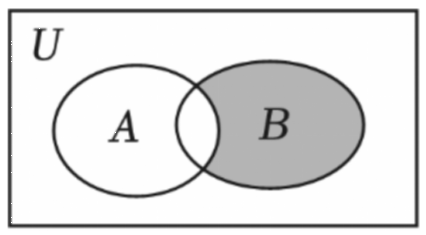
\includegraphics[width=0.26\textwidth]{figures/gao76_q14_venn.png}
\end{center}

\keepwithprev
A. $\{x\mid-2\leqslant x<4\}$\qquad B. $\{x\mid-1\leqslant x\leqslant3\}$

C. $\{x\mid x\leqslant3\text{ 或 }x\geqslant4\}$\qquad D. $\{x\mid-2\leqslant x\leqslant4\}$

\ifanswer
\solbegin
\step{全集 $U=\R$，集合 $A=\{x\mid x<-1\text{ 或 }x>4\}$，}
\step{$B=\{x\mid x^2-x-6\leqslant0\}=\{x\mid-2\leqslant x\leqslant3\}$，故 $A\cap B=\{x\mid-2\leqslant x<-1\}$，}
\step{故阴影部分表示的集合为 $\overline{A\cap B}=\{x\mid-1\leqslant x\leqslant3\}$. 故选 $B$.}
\solend
\fi

\item 设 $a$、$b$、$c\in\R$，给出下列命题：①若 $a>b$，则 $a^2>b^2$，②“$a>b$”是“$a^3>b^3$”的充要条件，③若 $a^2>b^2$，则 $|a|>|b|$，④若 $\dfrac ab>1$，则 $a>b$，⑤若 $a>b$，$c\neq0$，则 $\dfrac a{c^2}>\dfrac b{c^2}$，其中真命题的个数是\mbox{（\quad）}

\keepwithprev
A. $1$ 个\qquad B. $2$ 个\qquad C. $3$ 个\qquad D. $4$ 个

\ifanswer
\solbegin
\step{对于①，取 $a=2$，$b=-2$，满足 $a>b$，而 $a^2=b^2$，故为假命题；}
\step{对于②，$a>b\Leftrightarrow a^3-b^3=(a-b)(a^2+ab+b^2)=(a-b)\left[\left(a+\dfrac12b\right)^2+\dfrac34b^2\right]>0$}
\step{$\Leftrightarrow a^3>b^3$，故为真命题；}
\step{对于③，$a^2>b^2\Leftrightarrow|a|^2>|b|^2\Leftrightarrow|a|>|b|$，故为真命题；}
\step{对于④，取 $a=-2$，$b=-1$，满足 $\dfrac ab>1$，而 $a<b$，故为假命题；}
\step{对于⑤，由题意得 $c^2>0$，由 $a>b$，则 $\dfrac a{c^2}>\dfrac b{c^2}$，故为真命题.}
\step{故选 $C$.}
\solend
\fi

\item 已知关于 $x$ 的两个一元二次不等式 $a_1x^2+b_1x+c_1>0$，$a_2x^2+b_2x+c_2>0$ 的解集分别为 $A$、$B$，其中 $a_i$、$b_i$、$c_i(i=1,2)$ 为常数且不为零，则“$\dfrac{a_1}{a_2}=\dfrac{b_1}{b_2}=\dfrac{c_1}{c_2}$”是“$A=B$”\mbox{（\quad）}

\keepwithprev
A. 充分不必要条件\qquad B. 必要不充分条件

C. 充要条件\qquad D. 既不充分也不必要条件

\ifanswer
\solbegin
\step{设 $\dfrac{a_1}{a_2}=\dfrac{b_1}{b_2}=\dfrac{c_1}{c_2}=\lambda$，}
\step{①当 $\lambda>0$ 时，则 $a_1=\lambda a_2$，$b_1=\lambda b_2$，$c_1=\lambda c_2$，}
\step{$a_1x^2+b_1x+c_1>0\Leftrightarrow\lambda a_2x^2+\lambda b_2x+\lambda c_2>0\Leftrightarrow a_2x^2+b_2x+c_2>0$，}
\step{所以 $A=B$，}
\step{②当 $\lambda<0$ 时，则 $a_1=\lambda a_2$，$b_1=\lambda b_2$，$c_1=\lambda c_2$，}
\step{$a_1x^2+b_1x+c_1>0\Leftrightarrow\lambda a_2x^2+\lambda b_2x+\lambda c_2>0\Leftrightarrow a_2x^2+b_2x+c_2<0$，}
\step{所以 $A\neq B$，充分性不成立，}
\step{当 $A=B=\R$ 时，则 $\Delta<0$ 且 $a_1$、$a_2>0$，$\dfrac{a_1}{a_2}=\dfrac{b_1}{b_2}=\dfrac{c_1}{c_2}$ 不一定成立，}
\step{必要性不成立.}
\step{所以 $\dfrac{a_1}{a_2}=\dfrac{b_1}{b_2}=\dfrac{c_1}{c_2}$ 是 $A=B$ 的既不充分也不必要条件，故选 $D$.}
\solend
\fi

\end{enumerate}

\bigsec{三、解答题}

\begin{enumerate}
\setcounter{enumi}{16}

\item 求下列关于 $x$ 的不等式（组）的解集.

（1）$\begin{cases}9x^2-6x-24>0\\ \dfrac{x+3}{x-1}>2\end{cases}$；

（2）$|2x+1|-|2-x|>2$.

\ifanswer
\solbegin
\stepm{(1)}{不等式 $\dfrac{x+3}{x-1}>2$ 可化为 $\dfrac{x+3}{x-1}-2>0$，}
\step{即 $\dfrac{-x+5}{x-1}>0$，即 $(x-1)(x-5)<0$，解得 $1<x<5$，}
\step{不等式 $9x^2-6x-24>0$ 可化为 $(3x+4)(x-2)>0$，}
\step{解得 $x<-\dfrac43$ 或 $x>2$，}
\step{所以不等式的解集为 $(2,5)$.}
\stepm{(2)}{当 $x\leqslant-\dfrac12$ 时，$|2x+1|-|2-x|>2$ 等价于 $-2x-1-(2-x)>2$，}
\step{解得 $x<-5$，所以 $x<-5$，}
\step{当 $-\dfrac12<x<2$ 时，$|2x+1|-|2-x|>2$ 等价于 $2x+1-(2-x)>2$，}
\step{解得 $x>1$，所以 $1<x<2$，}
\step{当 $x\geqslant2$ 时，$|2x+1|-|2-x|>2$ 等价于 $2x+1-(x-2)>2$，}
\step{解得 $x>-1$，所以 $x\geqslant2$，}
\step{综上，$|2x+1|-|2-x|>2$ 的解集为 $(-\infty,-5)\cup(1,+\infty)$.}
\solend
\fi

\ansspace

\item 设 $m$ 为实数，求关于 $x$ 与 $y$ 的二元一次方程组 $\begin{cases}y=x+m\\ mx-y=4\end{cases}$ 的解集.

\ifanswer
\solbegin
\step{消去 $y$ 得 $(m-1)x=m+4$，}
\step{当 $m-1=0$，即 $m=1$ 时，$0=5$ 不成立，则 $x$ 无解，原方程组的解集为 $\varnothing$；}
\step{当 $m-1\neq0$，即 $m\neq1$ 时，则 $x=\dfrac{m+4}{m-1}$，$y=\dfrac{m+4}{m-1}+m=\dfrac{m^2+4}{m-1}$，}
\step{原方程组的解集为 $\left\{\left(\dfrac{m+4}{m-1},\dfrac{m^2+4}{m-1}\right)\right\}$.}
\step{综上所述，当 $m=1$ 时，方程组的解集为 $\varnothing$；}
\step{当 $m\neq1$ 时，方程组的解集为 $\left\{\left(\dfrac{m+4}{m-1},\dfrac{m^2+4}{m-1}\right)\right\}$.}
\solend
\fi

\ansspace

\item 已知集合 $A=\{x\mid-2\leqslant x-1\leqslant5\}$，集合 $B=\{x\mid m+1\leqslant x\leqslant2m-1\}(m\in\R)$.

（1）若 $m=4$，全集 $U=\R$，求 $A\cap B$；

（2）设命题 $p:x\in A$；命题 $q:x\in B$，若命题 $p$ 是命题 $q$ 的必要不充分条件，求实数 $m$ 的取值范围.

\ifanswer
\solbegin
\stepm{(1)}{由题意得 $A=\{x\mid-2\leqslant x-1\leqslant5\}=\{x\mid-1\leqslant x\leqslant6\}$，}
\step{当 $m=4$ 时，$B=\{x\mid5\leqslant x\leqslant7\}$，$A\cap B=\{x\mid5\leqslant x\leqslant6\}$；}
\stepm{(2)}{因为命题 $p$ 是命题 $q$ 的必要不充分条件，所以集合 $B$ 是集合 $A$ 的真子集，}
\step{当 $B=\varnothing$ 时，$m+1>2m-1$，解得 $m<2$，}
\step{当 $B\neq\varnothing$ 时，$\begin{cases}m+1\leqslant2m-1\\ m+1\geqslant-1\\ 2m-1\leqslant6\end{cases}$（等号不能同时成立），解得 $2\leqslant m\leqslant\dfrac72$，}
\step{综上所述，实数 $m$ 的取值范围为 $\left(-\infty,\dfrac72\right]$.}
\solend
\fi

\ansspace

\item （1）已知实数 $x\neq0$，求 $x+\dfrac1x$ 的取值范围；

（2）如图，要设计一张矩形海报，该海报含有大小相等的左右两个矩形栏目（即图中阴影部分），这两栏的面积之和为 $18000\,\mathrm{cm}^2$，四周空白的宽度为 $10\,\mathrm{cm}$，两栏之间的中缝空白的宽度为 $16\,\mathrm{cm}$，怎样确定海报的高与宽的尺寸（单位：$\mathrm{cm}$），能使矩形海报面积 $S$ 最小？最小面积是多少？

\begin{center}
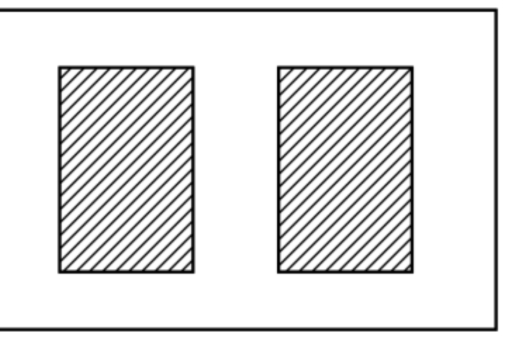
\includegraphics[width=0.34\textwidth]{figures/gao76_q20_poster.png}
\end{center}

\ifanswer
\solbegin
\stepm{(1)}{当 $x>0$ 时，$x+\dfrac1x\geqslant2\sqrt{x\times\dfrac1x}=2$，当且仅当 $x=\dfrac1x$，即 $x=1$ 取等号，}
\step{当 $x<0$ 时，$-x-\dfrac1x\geqslant2\sqrt{(-x)\times\dfrac1{-x}}=2$，所以 $x+\dfrac1x\leqslant-2$，}
\step{当且仅当 $-x=-\dfrac1x$，即 $x=-1$ 取等号，}
\step{综上所述，$x+\dfrac1x$ 的取值范围为 $(-\infty,-2]\cup[2,+\infty)$.}
\stepm{(2)}{设矩形栏目宽为 $x$，高为 $y$，则 $2xy=18000$，}
\step{所以 $S=(2x+36)(y+20)=2xy+36y+40x+720$}
% 原卷此行把 18720 写作 36720，照录（见文件头“原卷笔误/存疑”①）
\step{$=18000+36y+40x+720\geqslant18720+2\sqrt{36y\times40x}$}
\step{$=36720+2\sqrt{36\times40\times18000}=18720+7200=25920$，}
\step{当且仅当 $36y=40x$，即 $x=90$，$y=100$ 取等号，}
\step{所以海报的高为 $120\,\mathrm{cm}$ 与宽为 $216\,\mathrm{cm}$，可使矩形海报面积 $S$ 最小，}
\step{最小面积为 $25920$.}
\solend
\fi

\ansspace

\item 若实数 $x$、$y$、$m$ 满足 $|x-m|>|y-m|$，则称 $x$ 比 $y$ 远离 $m$.

（1）$0$ 比 $\dfrac12$ 远离 $2$ 吗？说明理由；

（2）若 $\dfrac1{2x-1}$ 比 $\dfrac12$ 远离 $1$，求实数 $x$ 的取值范围；

（3）若 $m\leqslant1$，$x+y=2$，试问：$x$ 与 $x^2+y^2$ 哪一个更远离 $m$，并说明理由.

\ifanswer
\solbegin
\stepm{(1)}{$0$ 比 $\dfrac12$ 远离 $2$，理由为：}
\step{由于 $|0-2|=2>\dfrac32=\left|\dfrac12-2\right|$，所以 $0$ 比 $\dfrac12$ 远离 $2$.}
\stepm{(2)}{由 $\dfrac1{2x-1}$ 比 $\dfrac12$ 远离 $1$，得 $\left|\dfrac1{2x-1}-1\right|>\left|\dfrac12-1\right|$，即 $\left|\dfrac1{2x-1}-1\right|>\dfrac12$，}
\step{则 $\dfrac1{2x-1}-1>\dfrac12$ 或 $\dfrac1{2x-1}-1<-\dfrac12$，整理得 $\dfrac1{2x-1}>\dfrac32$ 或 $\dfrac1{2x-1}<\dfrac12$，}
\step{因此 $0<2x-1<\dfrac23$ 或 $2x-1<0$ 或 $2x-1>2$，}
\step{解得 $\dfrac12<x<\dfrac56$ 或 $x<\dfrac12$ 或 $x>\dfrac32$，}
\step{所以 $x$ 的取值范围是 $\left(-\infty,\dfrac12\right)\cup\left(\dfrac12,\dfrac56\right)\cup\left(\dfrac32,+\infty\right)$.}
\stepm{(3)}{$x^2+y^2$ 比 $x$ 更远离 $m$，理由为：}
\step{由 $x^2+y^2\geqslant\dfrac{(x+y)^2}2=2\geqslant m$，得 $|x^2+y^2-m|=x^2+y^2-m$，}
\step{由 $x+y=2$，得 $x^2+y^2=x^2+(2-x)^2=2x^2-4x+4$，}
\step{于是 $|x^2+y^2-m|-|x-m|=2x^2-4x+4-m-|x-m|$，}
\step{当 $x\geqslant m$ 时，$|x^2+y^2-m|-|x-m|=2x^2-4x+4-m-(x-m)$}
\step{$=2\left(x-\dfrac54\right)^2+\dfrac78>0$，即 $|x^2+y^2-m|>|x-m|$；}
\step{当 $x<m$ 时，$|x^2+y^2-m|-|x-m|=2x^2-4x+4-m+(x-m)$}
\step{$=2\left(x-\dfrac34\right)^2+\dfrac{23}8-2m$，}
\step{由 $m\leqslant1$，得 $\dfrac{23}8-2m>0$，因此 $2\left(x-\dfrac34\right)^2+\dfrac{23}8-2m>0$，}
\step{即 $|x^2+y^2-m|>|x-m|$，}
\step{所以 $|x^2+y^2-m|>|x-m|$，即 $x^2+y^2$ 比 $x$ 更远离 $m$.}
\solend
\fi

\ansspace*[7]

\end{enumerate}

\end{document}
"
% 紧凑版：xelatex "\def\iscompact{1}% 高一76_六十中学_10月月考.tex
%   —— 高一上数学“2026-2027 年六十中学高一上 10 月月考”（讲评版）
% 试卷版：xelatex 高一76_六十中学_10月月考.tex
% 答案版：xelatex "\def\isanswer{1}% 高一76_六十中学_10月月考.tex
%   —— 高一上数学“2026-2027 年六十中学高一上 10 月月考”（讲评版）
% 试卷版：xelatex 高一76_六十中学_10月月考.tex
% 答案版：xelatex "\def\isanswer{1}\input{高一76_六十中学_10月月考.tex}"
% 紧凑版：xelatex "\def\iscompact{1}\input{高一76_六十中学_10月月考.tex}"
%
% 原始材料：微信公众号“魔都数学加油站”文章，连载“27学年高一76”；
% 原文标题“27学年高一76——2026-2027年上海市六十中学高一上10月月考”；
% 原文链接：https://mp.weixin.qq.com/s/GrKZjQrV1Xb0wy0BUuzAHw。
% 页面标注发布时间 2026-10-22 21:45（上海）。
% 正文为 10 张 PNG 页（`原图/高一76_六十中学_10月月考/01..10.png`）：
% 第 4、5、8、9 页为 4762×6735，其余 6 页为 2560×3620，均按页序读取。
% 10 页全为试卷正文页（卷首标题在第 1 页页顶，卷末第 21 题 (3) 解析止于第 10 页），
% 无封面页、目录页、二维码或宣传页。粉色斜排“魔都数学加油站”为卷面水印，未录入。
%
% 卷首标题：照卷面印作“2026-2027 年六十中学高一上 10 月月考”（黑体加粗一行）。
% 原卷年份区间用半角连字符，本稿按全稿惯例排 en dash；原卷无副标题。
%
% 篇幅与题号：原卷自第 3 题起编号（第 1、2 题不在本卷内）。填空题 3—12（10 题）、
% 选择题 13—16（4 题）、解答题 17—21（5 题），共 19 题。本稿沿用原节与原题号，
% 只改排为全稿统一的大节样式。
%
% 讲评版：原卷第 3、5 题只印【答案】（“$(0,1)$”“$a$、$b$ 都不能被 $3$ 整除”），
% 本稿只给 \ans{}；其余 17 题均印【解析】，用 \solbegin…\solend。四道选择题的作答
% 括号原卷即留空，答案写在解析末句“故选 C／B／C／D”，照录在解析内，不另提 \ans{}。
%
% 副标题：原卷未印副标题。本稿按“知识模块”口径标作“集合与常用逻辑用语、不等式”：
% 19 题中集合与常用逻辑用语 6 题（第 5、12、14、16、19 题及第 4 题的恒等变形），
% 不等式 13 题（第 3、6—11、13、15、17、18、20、21 题），两类均确有分量，故并标。
% 口径同 高一63、高一68—75。
%
% 与原卷的排版差异：
%   ① 原卷每题下直接印【答案】/【解析】，本稿按全稿惯例将答案与解析置于答案版；
%   ② 原卷未印副标题，本稿按“知识模块”口径补出；
%   ③ 原卷填空横线约四个字宽，本稿按全稿惯例统一排 \blankline[4.4em]；
%   ④ 原卷数集记号排斜体 $R$、$N$（第 4、6、7、8、11、12、14、15、19、20 题），本稿
%      按全稿惯例改用 $\R$、$\N$（同 高一68—75）；第 7、19、20 题的“解集为 $\R$”同此；
%   ⑤ 原卷句末标点多为西文句点，均逐处照录；
%   ⑥ 第 17—21 题的子问原卷印作“（1）…（2）…”，本稿按 高一69—75 成例用行内
%      “（1）（2）（3）”段，解析中的子问标号用 \stepm{(1)}{…}；
%   ⑦ 每道解答题原卷未留作答空白，本稿按全稿惯例加 \ansspace（末题用 \ansspace*）；
%   ⑧ 选择题的作答括号原卷排半角“(    )”，本稿按全稿惯例排 \mbox{（\quad）}；
%      选项行排照原卷——第 13、14、15、16 题一行两条、分两行排（本稿按原卷分行）；
%   ⑨ 第 10、11、17—21 题解析中的不等式组／方程组，原卷均排作“{”连接的多行式，
%      本稿按全稿惯例排 cases；
%   ⑩ 第 14 题题干右侧有一幅韦恩图（全集矩形内含 A、B 两圆，B 涂灰）：本稿按原卷
%      截图裁取（`figures/gao76_q14_venn.png`，由第 5 页原图裁出、去除粉色水印后转
%      灰度，未放大），放在题干之后、选项之前，仅答案版出；
%   ⑪ 第 20 题 (2) 题干右侧有一幅示意图（大矩形内两个斜线阴影小矩形）：本稿按原卷
%      截图裁取（`figures/gao76_q20_poster.png`，由第 8 页原图裁出、去除粉色水印后转
%      灰度，未放大），放在该小题文字之后，仅答案版出。
%
% 原卷笔误/存疑（均照录未改，正文对应处另有 % 注）：
%   ① 第 20 题 (2) 解析第 3 行把 $2xy+720$ 写成 $36720$（实为 $18000+720=18720$），
%      同式下一行又写回 $18720$，前后不一致；原卷如此，照录未改。
%   ② 第 14 题的韦恩图阴影是把整个 $B$ 圆（含 $A\cap B$ 部分）涂灰，而解析按
%      $\overline{A\cap B}$ 求解，二者不一致；原卷图文如此，照录未改。
%
% 行数核对：逐题数 \step/\stepm 条数与原卷【解析】印刷行数，17 题逐一相符，
% 合计 118 条 / 118 行（Q4：3；Q6：4；Q7：1；Q8：6；Q9：3；Q10：7；Q11：4；
% Q12：16；Q13：1；Q14：3；Q15：7；Q16：10；Q17：12；Q18：6；Q19：6；Q20：11；
% Q21：18）。另第 3、5 题只印【答案】，各提 \ans{}，不计入 \step 账。
%
% 插图：第 14 题题干的韦恩图、第 20 题 (2) 的示意图，见上⑩⑪；其余题干无配图。
%
\documentclass[a4paper,11pt]{article}
\usepackage{common}

\begin{document}

\examtitlest[3]{2026--2027 年六十中学高一上 10 月月考}{集合与常用逻辑用语、不等式}

\bigsec{一、填空题}

\begin{enumerate}
\setcounter{enumi}{2}

\item 不等式 $\dfrac{x}{1-x}>0$ 的解集是\blankline[4.4em].

\ifanswer
\ans{$(0,1)$}
\fi

\item 已知 $2x^2+x+1=a(x+1)^2+b(x+1)+2$，对 $x\in\R$ 恒成立，$ab=$\blankline[4.4em].

\ifanswer
\solbegin
\step{若 $2x^2+x+1=a(x+1)^2+b(x+1)+2$ 对 $x\in\R$ 恒成立，}
\step{即 $2x^2+x+1=ax^2+(2a+b)x+a+b+2$ 对 $x\in\R$ 恒成立，}
\step{必有 $\begin{cases}a=2\\ 2a+b=1\\ a+b+2=1\end{cases}$，解得 $a=2$，$b=-3$，所以 $ab=-6$.}
\solend
\fi

\item 利用反证法证明命题：“如果 $a$、$b\in\N$，$ab$ 可被 $3$ 整除，那么 $a$、$b$ 中至少有一个能被 $3$ 整除”时，假设的内容应是\blankline[4.4em].

\ifanswer
\ans{$a$、$b$ 都不能被 $3$ 整除}
\fi

\item 已知 $x\in\R$，方程 $|x+1|+|2-x|=3$ 的解集为\blankline[4.4em].

\ifanswer
\solbegin
\step{当 $x<-1$ 时，则 $|x+1|+|2-x|=-x-1+2-x=1-2x>3$；}
\step{当 $-1\leqslant x\leqslant2$ 时，则 $|x+1|+|2-x|=x+1+2-x=3$；}
\step{当 $x>2$ 时，则 $|x+1|+|2-x|=x+1+x-2=2x-1>3$.}
\step{综上所述，原方程的解集为 $[-1,2]$.}
\solend
\fi

\item 若关于 $x$ 的不等式 $x^2+kx+1\geqslant0$ 的解集为 $\R$，则实数 $k$ 的取值范围是\blankline[4.4em].

\ifanswer
\solbegin
\step{$\Delta=k^2-4\leqslant0\Rightarrow-2\leqslant k\leqslant2$，所以实数 $k$ 的取值范围是 $[-2,2]$.}
\solend
\fi

\item 已知 $a$、$b\in\R$，且 $ab>0$，则下列不等式中，恒成立的序号是\blankline[4.4em].

① $a^2+b^2>2ab$；② $a+b\geqslant2\sqrt{ab}$；③ $\dfrac1a+\dfrac1b>\dfrac2{\sqrt{ab}}$；④ $\dfrac ba+\dfrac ab\geqslant2$.

\ifanswer
\solbegin
\step{因为 $a^2+b^2\geqslant2ab$ 对于 $a$、$b\in\R$ 恒成立，当且仅当 $a=b$ 时取等号，}
\step{所以①错误；}
\step{对于②，③，显然 $a<0$，$b<0$ 时，不等式均不成立，即②和③错误；}
\step{对于④，因为 $ab>0$，所以 $\dfrac ba>0,\dfrac ab>0$，}
\step{由基本不等式得 $\dfrac ba+\dfrac ab\geqslant2\sqrt{\dfrac ba\cdot\dfrac ab}=2$，即④正确.}
\step{故正确的是④.}
\solend
\fi

\item 已知正实数 $m$、$n$ 满足 $m+\dfrac2n=1$，则 $\dfrac1m+2n$ 的最小值为\blankline[4.4em].

\ifanswer
\solbegin
\step{$\dfrac1m+2n=\left(m+\dfrac2n\right)\left(\dfrac1m+2n\right)=5+2mn+\dfrac2{mn}$，}
\step{因为 $mn>0$，所以 $2mn+\dfrac2{mn}\geqslant2\sqrt{2mn\cdot\dfrac2{mn}}=4$，}
\step{当且仅当 $2mn=\dfrac2{mn}$，即 $m=\dfrac13$，$n=3$ 时取等号，所以 $\dfrac1m+2n$ 的最小值为 $9$.}
\solend
\fi

\item 若关于 $x$ 的不等式组 $\begin{cases}3x+1>0\\ x+\dfrac1a\leqslant2\end{cases}$ 恰好有两个整数解，则实数 $a$ 的取值范围为\blankline[4.4em].

\ifanswer
\solbegin
\step{由 $3x+1>0$ 得 $x>-\dfrac13$；若 $a<0$，则 $\dfrac1a<0$，由 $x+\dfrac1a\leqslant2$ 得 $x\leqslant2-\dfrac1a>2$，}
\step{则解集 $\left(-\dfrac13,2-\dfrac1a\right]$ 必同时含有整数 $0$、$1$、$2$，不合题意；}
\step{又 $a=0$ 使 $\dfrac1a$ 无意义，故 $a>0$；}
\step{此时原不等式组的解集为 $\left(-\dfrac13,2-\dfrac1a\right]$，}
\step{其中大于 $-\dfrac13$ 的整数依次为 $0$，$1$，$2$，$\cdots$，}
\step{恰有两个整数解即解集只含 $0$ 与 $1$，故 $1\leqslant2-\dfrac1a<2$，即 $\dfrac1a\leqslant1$ 且 $\dfrac1a>0$，}
\step{结合 $a>0$，解得 $a\geqslant1$.}
\solend
\fi

\item 已知 $a\in\R$，若关于 $x$ 的方程 $x^2+ax+a^2-8=0$ 有两个实根 $x_1$、$x_2$，且 $\dfrac1{x_1}+\dfrac1{x_2}=-\dfrac12$，则 $a$ 的值为\blankline[4.4em].

\ifanswer
\solbegin
\step{由题意得 $\Delta=a^2-4(a^2-8)=32-3a^2\geqslant0$，解得 $a^2\leqslant\dfrac{32}3$，}
\step{由韦达定理得 $x_1+x_2=-a$，$x_1x_2=a^2-8$，}
\step{则 $\dfrac1{x_1}+\dfrac1{x_2}=\dfrac{x_1+x_2}{x_1x_2}=\dfrac{-a}{a^2-8}=-\dfrac12$，即 $a^2-2a-8=(a-4)(a+2)=0$，}
\step{解得 $a=4$ 或 $a=-2$，又 $a^2\leqslant\dfrac{32}3$，则 $a=-2$.}
\solend
\fi

\item 已知有限集 $A=\{a_1,a_2,\cdots,a_n\}(n\geqslant2,n\in\N)$，若 $A$ 中元素 $a_i(i=1,2,\cdots,n)$ 满足 $a_1+a_2+\cdots+a_n=a_1\times a_2\times\cdots\times a_n$，就称 $A$ 为“完美集”，以下四个命题：

①集合 $\{-1-\sqrt3,-1+\sqrt3\}$ 不是“完美集”；

②若 $a_1$、$a_2$ 是两个不同的正数，且 $\{a_1,a_2\}$ 是“完美集”，则 $a_1$、$a_2$ 至少有一个大于 $2$；

③二元“完美集”有无穷多个；

④若 $a_i$ 均为正整数，则“完美集”$A$ 有且只有一个，且 $n=3$.

其中，真命题的序号是\blankline[4.4em].

\ifanswer
\solbegin
\step{对于①选项：$(-1-\sqrt3)+(-1+\sqrt3)=-2$，$(-1-\sqrt3)\times(-1+\sqrt3)=-2$，}
\step{故 $(-1-\sqrt3)+(-1+\sqrt3)=(-1-\sqrt3)\times(-1+\sqrt3)$，}
\step{所以集合 $\{-1-\sqrt3,-1+\sqrt3\}$ 是“完美集”，故①错误；}
\step{对于②选项：集合 $\{a_1,a_2\}$ 是“完美集”，设 $a_1+a_2=a_1a_2=t>0$，}
\step{则 $a_1$、$a_2$ 可以看成一元二次方程 $x^2-tx+t=0$ 的两正根，则 $\Delta=t^2-4t>0$，}
\step{解得 $t<0$（舍）或 $t>4$，即 $a_1a_2>4$，所以至少有一个大于 $2$，故②正确；}
\step{对于③选项：由②得一元二次方程 $x^2-tx+t=0$ 当 $t$ 取不同值时，}
\step{$a_1$、$a_2$ 的值是不同的，因而二元“完美集”有无穷多个，故③正确；}
\step{对于④选项：设 $a_1<a_2<a_3<\cdots<a_n$，}
\step{则 $a_1\times a_2\times\cdots\times a_n=a_1+a_2+\cdots+a_n<na_n$，}
\step{所以 $a_1\times a_2\times\cdots\times a_{n-1}<n$，又 $a_i\in\N^*$，所以 $n\leqslant3$，}
\step{当 $n=2$ 时，$a_1<2$，则 $a_1=1$，$a_1a_2\neq a_1+a_2$，不合题意，}
\step{当 $n=3$ 时，$a_1a_2<3$，所以只能是 $a_1=1$，$a_2=2$，}
\step{由 $a_1+a_2+a_3=a_1a_2a_3$，代入解得 $a_3=3$，所以此时“完美集”只有一个，}
\step{为 $\{1,2,3\}$，故④正确.}
\step{故正确的是②③④.}
\solend
\fi

\end{enumerate}

\bigsec{二、选择题}

\begin{enumerate}
\setcounter{enumi}{12}

\item 已知 $x$、$y\in\R$，则“$xy\geqslant0$”是“$xy=|xy|$”的\mbox{（\quad）}

\keepwithprev
A. 充分非必要条件\qquad B. 必要非充分条件

C. 充要条件\qquad D. 既非充分也非必要条件

\ifanswer
\solbegin
\step{$xy\geqslant0\Leftrightarrow xy=|xy|$，故“$xy\geqslant0$”是“$xy=|xy|$”的充要条件. 故选 $C$.}
\solend
\fi

\needvspace{22\baselineskip}
\item 已知全集 $U=\R$，集合 $A=\{x\mid x<-1\text{ 或 }x>4\}$，$B=\{x\mid x^2-x-6\leqslant0\}$，则阴影部分表示的集合为\mbox{（\quad）}

\begin{center}
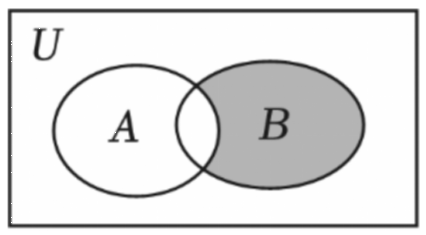
\includegraphics[width=0.26\textwidth]{figures/gao76_q14_venn.png}
\end{center}

\keepwithprev
A. $\{x\mid-2\leqslant x<4\}$\qquad B. $\{x\mid-1\leqslant x\leqslant3\}$

C. $\{x\mid x\leqslant3\text{ 或 }x\geqslant4\}$\qquad D. $\{x\mid-2\leqslant x\leqslant4\}$

\ifanswer
\solbegin
\step{全集 $U=\R$，集合 $A=\{x\mid x<-1\text{ 或 }x>4\}$，}
\step{$B=\{x\mid x^2-x-6\leqslant0\}=\{x\mid-2\leqslant x\leqslant3\}$，故 $A\cap B=\{x\mid-2\leqslant x<-1\}$，}
\step{故阴影部分表示的集合为 $\overline{A\cap B}=\{x\mid-1\leqslant x\leqslant3\}$. 故选 $B$.}
\solend
\fi

\item 设 $a$、$b$、$c\in\R$，给出下列命题：①若 $a>b$，则 $a^2>b^2$，②“$a>b$”是“$a^3>b^3$”的充要条件，③若 $a^2>b^2$，则 $|a|>|b|$，④若 $\dfrac ab>1$，则 $a>b$，⑤若 $a>b$，$c\neq0$，则 $\dfrac a{c^2}>\dfrac b{c^2}$，其中真命题的个数是\mbox{（\quad）}

\keepwithprev
A. $1$ 个\qquad B. $2$ 个\qquad C. $3$ 个\qquad D. $4$ 个

\ifanswer
\solbegin
\step{对于①，取 $a=2$，$b=-2$，满足 $a>b$，而 $a^2=b^2$，故为假命题；}
\step{对于②，$a>b\Leftrightarrow a^3-b^3=(a-b)(a^2+ab+b^2)=(a-b)\left[\left(a+\dfrac12b\right)^2+\dfrac34b^2\right]>0$}
\step{$\Leftrightarrow a^3>b^3$，故为真命题；}
\step{对于③，$a^2>b^2\Leftrightarrow|a|^2>|b|^2\Leftrightarrow|a|>|b|$，故为真命题；}
\step{对于④，取 $a=-2$，$b=-1$，满足 $\dfrac ab>1$，而 $a<b$，故为假命题；}
\step{对于⑤，由题意得 $c^2>0$，由 $a>b$，则 $\dfrac a{c^2}>\dfrac b{c^2}$，故为真命题.}
\step{故选 $C$.}
\solend
\fi

\item 已知关于 $x$ 的两个一元二次不等式 $a_1x^2+b_1x+c_1>0$，$a_2x^2+b_2x+c_2>0$ 的解集分别为 $A$、$B$，其中 $a_i$、$b_i$、$c_i(i=1,2)$ 为常数且不为零，则“$\dfrac{a_1}{a_2}=\dfrac{b_1}{b_2}=\dfrac{c_1}{c_2}$”是“$A=B$”\mbox{（\quad）}

\keepwithprev
A. 充分不必要条件\qquad B. 必要不充分条件

C. 充要条件\qquad D. 既不充分也不必要条件

\ifanswer
\solbegin
\step{设 $\dfrac{a_1}{a_2}=\dfrac{b_1}{b_2}=\dfrac{c_1}{c_2}=\lambda$，}
\step{①当 $\lambda>0$ 时，则 $a_1=\lambda a_2$，$b_1=\lambda b_2$，$c_1=\lambda c_2$，}
\step{$a_1x^2+b_1x+c_1>0\Leftrightarrow\lambda a_2x^2+\lambda b_2x+\lambda c_2>0\Leftrightarrow a_2x^2+b_2x+c_2>0$，}
\step{所以 $A=B$，}
\step{②当 $\lambda<0$ 时，则 $a_1=\lambda a_2$，$b_1=\lambda b_2$，$c_1=\lambda c_2$，}
\step{$a_1x^2+b_1x+c_1>0\Leftrightarrow\lambda a_2x^2+\lambda b_2x+\lambda c_2>0\Leftrightarrow a_2x^2+b_2x+c_2<0$，}
\step{所以 $A\neq B$，充分性不成立，}
\step{当 $A=B=\R$ 时，则 $\Delta<0$ 且 $a_1$、$a_2>0$，$\dfrac{a_1}{a_2}=\dfrac{b_1}{b_2}=\dfrac{c_1}{c_2}$ 不一定成立，}
\step{必要性不成立.}
\step{所以 $\dfrac{a_1}{a_2}=\dfrac{b_1}{b_2}=\dfrac{c_1}{c_2}$ 是 $A=B$ 的既不充分也不必要条件，故选 $D$.}
\solend
\fi

\end{enumerate}

\bigsec{三、解答题}

\begin{enumerate}
\setcounter{enumi}{16}

\item 求下列关于 $x$ 的不等式（组）的解集.

（1）$\begin{cases}9x^2-6x-24>0\\ \dfrac{x+3}{x-1}>2\end{cases}$；

（2）$|2x+1|-|2-x|>2$.

\ifanswer
\solbegin
\stepm{(1)}{不等式 $\dfrac{x+3}{x-1}>2$ 可化为 $\dfrac{x+3}{x-1}-2>0$，}
\step{即 $\dfrac{-x+5}{x-1}>0$，即 $(x-1)(x-5)<0$，解得 $1<x<5$，}
\step{不等式 $9x^2-6x-24>0$ 可化为 $(3x+4)(x-2)>0$，}
\step{解得 $x<-\dfrac43$ 或 $x>2$，}
\step{所以不等式的解集为 $(2,5)$.}
\stepm{(2)}{当 $x\leqslant-\dfrac12$ 时，$|2x+1|-|2-x|>2$ 等价于 $-2x-1-(2-x)>2$，}
\step{解得 $x<-5$，所以 $x<-5$，}
\step{当 $-\dfrac12<x<2$ 时，$|2x+1|-|2-x|>2$ 等价于 $2x+1-(2-x)>2$，}
\step{解得 $x>1$，所以 $1<x<2$，}
\step{当 $x\geqslant2$ 时，$|2x+1|-|2-x|>2$ 等价于 $2x+1-(x-2)>2$，}
\step{解得 $x>-1$，所以 $x\geqslant2$，}
\step{综上，$|2x+1|-|2-x|>2$ 的解集为 $(-\infty,-5)\cup(1,+\infty)$.}
\solend
\fi

\ansspace

\item 设 $m$ 为实数，求关于 $x$ 与 $y$ 的二元一次方程组 $\begin{cases}y=x+m\\ mx-y=4\end{cases}$ 的解集.

\ifanswer
\solbegin
\step{消去 $y$ 得 $(m-1)x=m+4$，}
\step{当 $m-1=0$，即 $m=1$ 时，$0=5$ 不成立，则 $x$ 无解，原方程组的解集为 $\varnothing$；}
\step{当 $m-1\neq0$，即 $m\neq1$ 时，则 $x=\dfrac{m+4}{m-1}$，$y=\dfrac{m+4}{m-1}+m=\dfrac{m^2+4}{m-1}$，}
\step{原方程组的解集为 $\left\{\left(\dfrac{m+4}{m-1},\dfrac{m^2+4}{m-1}\right)\right\}$.}
\step{综上所述，当 $m=1$ 时，方程组的解集为 $\varnothing$；}
\step{当 $m\neq1$ 时，方程组的解集为 $\left\{\left(\dfrac{m+4}{m-1},\dfrac{m^2+4}{m-1}\right)\right\}$.}
\solend
\fi

\ansspace

\item 已知集合 $A=\{x\mid-2\leqslant x-1\leqslant5\}$，集合 $B=\{x\mid m+1\leqslant x\leqslant2m-1\}(m\in\R)$.

（1）若 $m=4$，全集 $U=\R$，求 $A\cap B$；

（2）设命题 $p:x\in A$；命题 $q:x\in B$，若命题 $p$ 是命题 $q$ 的必要不充分条件，求实数 $m$ 的取值范围.

\ifanswer
\solbegin
\stepm{(1)}{由题意得 $A=\{x\mid-2\leqslant x-1\leqslant5\}=\{x\mid-1\leqslant x\leqslant6\}$，}
\step{当 $m=4$ 时，$B=\{x\mid5\leqslant x\leqslant7\}$，$A\cap B=\{x\mid5\leqslant x\leqslant6\}$；}
\stepm{(2)}{因为命题 $p$ 是命题 $q$ 的必要不充分条件，所以集合 $B$ 是集合 $A$ 的真子集，}
\step{当 $B=\varnothing$ 时，$m+1>2m-1$，解得 $m<2$，}
\step{当 $B\neq\varnothing$ 时，$\begin{cases}m+1\leqslant2m-1\\ m+1\geqslant-1\\ 2m-1\leqslant6\end{cases}$（等号不能同时成立），解得 $2\leqslant m\leqslant\dfrac72$，}
\step{综上所述，实数 $m$ 的取值范围为 $\left(-\infty,\dfrac72\right]$.}
\solend
\fi

\ansspace

\item （1）已知实数 $x\neq0$，求 $x+\dfrac1x$ 的取值范围；

（2）如图，要设计一张矩形海报，该海报含有大小相等的左右两个矩形栏目（即图中阴影部分），这两栏的面积之和为 $18000\,\mathrm{cm}^2$，四周空白的宽度为 $10\,\mathrm{cm}$，两栏之间的中缝空白的宽度为 $16\,\mathrm{cm}$，怎样确定海报的高与宽的尺寸（单位：$\mathrm{cm}$），能使矩形海报面积 $S$ 最小？最小面积是多少？

\begin{center}
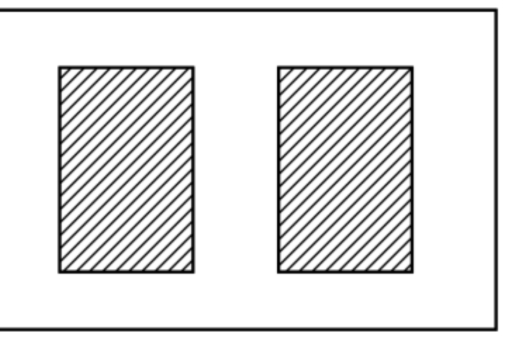
\includegraphics[width=0.34\textwidth]{figures/gao76_q20_poster.png}
\end{center}

\ifanswer
\solbegin
\stepm{(1)}{当 $x>0$ 时，$x+\dfrac1x\geqslant2\sqrt{x\times\dfrac1x}=2$，当且仅当 $x=\dfrac1x$，即 $x=1$ 取等号，}
\step{当 $x<0$ 时，$-x-\dfrac1x\geqslant2\sqrt{(-x)\times\dfrac1{-x}}=2$，所以 $x+\dfrac1x\leqslant-2$，}
\step{当且仅当 $-x=-\dfrac1x$，即 $x=-1$ 取等号，}
\step{综上所述，$x+\dfrac1x$ 的取值范围为 $(-\infty,-2]\cup[2,+\infty)$.}
\stepm{(2)}{设矩形栏目宽为 $x$，高为 $y$，则 $2xy=18000$，}
\step{所以 $S=(2x+36)(y+20)=2xy+36y+40x+720$}
% 原卷此行把 18720 写作 36720，照录（见文件头“原卷笔误/存疑”①）
\step{$=18000+36y+40x+720\geqslant18720+2\sqrt{36y\times40x}$}
\step{$=36720+2\sqrt{36\times40\times18000}=18720+7200=25920$，}
\step{当且仅当 $36y=40x$，即 $x=90$，$y=100$ 取等号，}
\step{所以海报的高为 $120\,\mathrm{cm}$ 与宽为 $216\,\mathrm{cm}$，可使矩形海报面积 $S$ 最小，}
\step{最小面积为 $25920$.}
\solend
\fi

\ansspace

\item 若实数 $x$、$y$、$m$ 满足 $|x-m|>|y-m|$，则称 $x$ 比 $y$ 远离 $m$.

（1）$0$ 比 $\dfrac12$ 远离 $2$ 吗？说明理由；

（2）若 $\dfrac1{2x-1}$ 比 $\dfrac12$ 远离 $1$，求实数 $x$ 的取值范围；

（3）若 $m\leqslant1$，$x+y=2$，试问：$x$ 与 $x^2+y^2$ 哪一个更远离 $m$，并说明理由.

\ifanswer
\solbegin
\stepm{(1)}{$0$ 比 $\dfrac12$ 远离 $2$，理由为：}
\step{由于 $|0-2|=2>\dfrac32=\left|\dfrac12-2\right|$，所以 $0$ 比 $\dfrac12$ 远离 $2$.}
\stepm{(2)}{由 $\dfrac1{2x-1}$ 比 $\dfrac12$ 远离 $1$，得 $\left|\dfrac1{2x-1}-1\right|>\left|\dfrac12-1\right|$，即 $\left|\dfrac1{2x-1}-1\right|>\dfrac12$，}
\step{则 $\dfrac1{2x-1}-1>\dfrac12$ 或 $\dfrac1{2x-1}-1<-\dfrac12$，整理得 $\dfrac1{2x-1}>\dfrac32$ 或 $\dfrac1{2x-1}<\dfrac12$，}
\step{因此 $0<2x-1<\dfrac23$ 或 $2x-1<0$ 或 $2x-1>2$，}
\step{解得 $\dfrac12<x<\dfrac56$ 或 $x<\dfrac12$ 或 $x>\dfrac32$，}
\step{所以 $x$ 的取值范围是 $\left(-\infty,\dfrac12\right)\cup\left(\dfrac12,\dfrac56\right)\cup\left(\dfrac32,+\infty\right)$.}
\stepm{(3)}{$x^2+y^2$ 比 $x$ 更远离 $m$，理由为：}
\step{由 $x^2+y^2\geqslant\dfrac{(x+y)^2}2=2\geqslant m$，得 $|x^2+y^2-m|=x^2+y^2-m$，}
\step{由 $x+y=2$，得 $x^2+y^2=x^2+(2-x)^2=2x^2-4x+4$，}
\step{于是 $|x^2+y^2-m|-|x-m|=2x^2-4x+4-m-|x-m|$，}
\step{当 $x\geqslant m$ 时，$|x^2+y^2-m|-|x-m|=2x^2-4x+4-m-(x-m)$}
\step{$=2\left(x-\dfrac54\right)^2+\dfrac78>0$，即 $|x^2+y^2-m|>|x-m|$；}
\step{当 $x<m$ 时，$|x^2+y^2-m|-|x-m|=2x^2-4x+4-m+(x-m)$}
\step{$=2\left(x-\dfrac34\right)^2+\dfrac{23}8-2m$，}
\step{由 $m\leqslant1$，得 $\dfrac{23}8-2m>0$，因此 $2\left(x-\dfrac34\right)^2+\dfrac{23}8-2m>0$，}
\step{即 $|x^2+y^2-m|>|x-m|$，}
\step{所以 $|x^2+y^2-m|>|x-m|$，即 $x^2+y^2$ 比 $x$ 更远离 $m$.}
\solend
\fi

\ansspace*[7]

\end{enumerate}

\end{document}
"
% 紧凑版：xelatex "\def\iscompact{1}% 高一76_六十中学_10月月考.tex
%   —— 高一上数学“2026-2027 年六十中学高一上 10 月月考”（讲评版）
% 试卷版：xelatex 高一76_六十中学_10月月考.tex
% 答案版：xelatex "\def\isanswer{1}\input{高一76_六十中学_10月月考.tex}"
% 紧凑版：xelatex "\def\iscompact{1}\input{高一76_六十中学_10月月考.tex}"
%
% 原始材料：微信公众号“魔都数学加油站”文章，连载“27学年高一76”；
% 原文标题“27学年高一76——2026-2027年上海市六十中学高一上10月月考”；
% 原文链接：https://mp.weixin.qq.com/s/GrKZjQrV1Xb0wy0BUuzAHw。
% 页面标注发布时间 2026-10-22 21:45（上海）。
% 正文为 10 张 PNG 页（`原图/高一76_六十中学_10月月考/01..10.png`）：
% 第 4、5、8、9 页为 4762×6735，其余 6 页为 2560×3620，均按页序读取。
% 10 页全为试卷正文页（卷首标题在第 1 页页顶，卷末第 21 题 (3) 解析止于第 10 页），
% 无封面页、目录页、二维码或宣传页。粉色斜排“魔都数学加油站”为卷面水印，未录入。
%
% 卷首标题：照卷面印作“2026-2027 年六十中学高一上 10 月月考”（黑体加粗一行）。
% 原卷年份区间用半角连字符，本稿按全稿惯例排 en dash；原卷无副标题。
%
% 篇幅与题号：原卷自第 3 题起编号（第 1、2 题不在本卷内）。填空题 3—12（10 题）、
% 选择题 13—16（4 题）、解答题 17—21（5 题），共 19 题。本稿沿用原节与原题号，
% 只改排为全稿统一的大节样式。
%
% 讲评版：原卷第 3、5 题只印【答案】（“$(0,1)$”“$a$、$b$ 都不能被 $3$ 整除”），
% 本稿只给 \ans{}；其余 17 题均印【解析】，用 \solbegin…\solend。四道选择题的作答
% 括号原卷即留空，答案写在解析末句“故选 C／B／C／D”，照录在解析内，不另提 \ans{}。
%
% 副标题：原卷未印副标题。本稿按“知识模块”口径标作“集合与常用逻辑用语、不等式”：
% 19 题中集合与常用逻辑用语 6 题（第 5、12、14、16、19 题及第 4 题的恒等变形），
% 不等式 13 题（第 3、6—11、13、15、17、18、20、21 题），两类均确有分量，故并标。
% 口径同 高一63、高一68—75。
%
% 与原卷的排版差异：
%   ① 原卷每题下直接印【答案】/【解析】，本稿按全稿惯例将答案与解析置于答案版；
%   ② 原卷未印副标题，本稿按“知识模块”口径补出；
%   ③ 原卷填空横线约四个字宽，本稿按全稿惯例统一排 \blankline[4.4em]；
%   ④ 原卷数集记号排斜体 $R$、$N$（第 4、6、7、8、11、12、14、15、19、20 题），本稿
%      按全稿惯例改用 $\R$、$\N$（同 高一68—75）；第 7、19、20 题的“解集为 $\R$”同此；
%   ⑤ 原卷句末标点多为西文句点，均逐处照录；
%   ⑥ 第 17—21 题的子问原卷印作“（1）…（2）…”，本稿按 高一69—75 成例用行内
%      “（1）（2）（3）”段，解析中的子问标号用 \stepm{(1)}{…}；
%   ⑦ 每道解答题原卷未留作答空白，本稿按全稿惯例加 \ansspace（末题用 \ansspace*）；
%   ⑧ 选择题的作答括号原卷排半角“(    )”，本稿按全稿惯例排 \mbox{（\quad）}；
%      选项行排照原卷——第 13、14、15、16 题一行两条、分两行排（本稿按原卷分行）；
%   ⑨ 第 10、11、17—21 题解析中的不等式组／方程组，原卷均排作“{”连接的多行式，
%      本稿按全稿惯例排 cases；
%   ⑩ 第 14 题题干右侧有一幅韦恩图（全集矩形内含 A、B 两圆，B 涂灰）：本稿按原卷
%      截图裁取（`figures/gao76_q14_venn.png`，由第 5 页原图裁出、去除粉色水印后转
%      灰度，未放大），放在题干之后、选项之前，仅答案版出；
%   ⑪ 第 20 题 (2) 题干右侧有一幅示意图（大矩形内两个斜线阴影小矩形）：本稿按原卷
%      截图裁取（`figures/gao76_q20_poster.png`，由第 8 页原图裁出、去除粉色水印后转
%      灰度，未放大），放在该小题文字之后，仅答案版出。
%
% 原卷笔误/存疑（均照录未改，正文对应处另有 % 注）：
%   ① 第 20 题 (2) 解析第 3 行把 $2xy+720$ 写成 $36720$（实为 $18000+720=18720$），
%      同式下一行又写回 $18720$，前后不一致；原卷如此，照录未改。
%   ② 第 14 题的韦恩图阴影是把整个 $B$ 圆（含 $A\cap B$ 部分）涂灰，而解析按
%      $\overline{A\cap B}$ 求解，二者不一致；原卷图文如此，照录未改。
%
% 行数核对：逐题数 \step/\stepm 条数与原卷【解析】印刷行数，17 题逐一相符，
% 合计 118 条 / 118 行（Q4：3；Q6：4；Q7：1；Q8：6；Q9：3；Q10：7；Q11：4；
% Q12：16；Q13：1；Q14：3；Q15：7；Q16：10；Q17：12；Q18：6；Q19：6；Q20：11；
% Q21：18）。另第 3、5 题只印【答案】，各提 \ans{}，不计入 \step 账。
%
% 插图：第 14 题题干的韦恩图、第 20 题 (2) 的示意图，见上⑩⑪；其余题干无配图。
%
\documentclass[a4paper,11pt]{article}
\usepackage{common}

\begin{document}

\examtitlest[3]{2026--2027 年六十中学高一上 10 月月考}{集合与常用逻辑用语、不等式}

\bigsec{一、填空题}

\begin{enumerate}
\setcounter{enumi}{2}

\item 不等式 $\dfrac{x}{1-x}>0$ 的解集是\blankline[4.4em].

\ifanswer
\ans{$(0,1)$}
\fi

\item 已知 $2x^2+x+1=a(x+1)^2+b(x+1)+2$，对 $x\in\R$ 恒成立，$ab=$\blankline[4.4em].

\ifanswer
\solbegin
\step{若 $2x^2+x+1=a(x+1)^2+b(x+1)+2$ 对 $x\in\R$ 恒成立，}
\step{即 $2x^2+x+1=ax^2+(2a+b)x+a+b+2$ 对 $x\in\R$ 恒成立，}
\step{必有 $\begin{cases}a=2\\ 2a+b=1\\ a+b+2=1\end{cases}$，解得 $a=2$，$b=-3$，所以 $ab=-6$.}
\solend
\fi

\item 利用反证法证明命题：“如果 $a$、$b\in\N$，$ab$ 可被 $3$ 整除，那么 $a$、$b$ 中至少有一个能被 $3$ 整除”时，假设的内容应是\blankline[4.4em].

\ifanswer
\ans{$a$、$b$ 都不能被 $3$ 整除}
\fi

\item 已知 $x\in\R$，方程 $|x+1|+|2-x|=3$ 的解集为\blankline[4.4em].

\ifanswer
\solbegin
\step{当 $x<-1$ 时，则 $|x+1|+|2-x|=-x-1+2-x=1-2x>3$；}
\step{当 $-1\leqslant x\leqslant2$ 时，则 $|x+1|+|2-x|=x+1+2-x=3$；}
\step{当 $x>2$ 时，则 $|x+1|+|2-x|=x+1+x-2=2x-1>3$.}
\step{综上所述，原方程的解集为 $[-1,2]$.}
\solend
\fi

\item 若关于 $x$ 的不等式 $x^2+kx+1\geqslant0$ 的解集为 $\R$，则实数 $k$ 的取值范围是\blankline[4.4em].

\ifanswer
\solbegin
\step{$\Delta=k^2-4\leqslant0\Rightarrow-2\leqslant k\leqslant2$，所以实数 $k$ 的取值范围是 $[-2,2]$.}
\solend
\fi

\item 已知 $a$、$b\in\R$，且 $ab>0$，则下列不等式中，恒成立的序号是\blankline[4.4em].

① $a^2+b^2>2ab$；② $a+b\geqslant2\sqrt{ab}$；③ $\dfrac1a+\dfrac1b>\dfrac2{\sqrt{ab}}$；④ $\dfrac ba+\dfrac ab\geqslant2$.

\ifanswer
\solbegin
\step{因为 $a^2+b^2\geqslant2ab$ 对于 $a$、$b\in\R$ 恒成立，当且仅当 $a=b$ 时取等号，}
\step{所以①错误；}
\step{对于②，③，显然 $a<0$，$b<0$ 时，不等式均不成立，即②和③错误；}
\step{对于④，因为 $ab>0$，所以 $\dfrac ba>0,\dfrac ab>0$，}
\step{由基本不等式得 $\dfrac ba+\dfrac ab\geqslant2\sqrt{\dfrac ba\cdot\dfrac ab}=2$，即④正确.}
\step{故正确的是④.}
\solend
\fi

\item 已知正实数 $m$、$n$ 满足 $m+\dfrac2n=1$，则 $\dfrac1m+2n$ 的最小值为\blankline[4.4em].

\ifanswer
\solbegin
\step{$\dfrac1m+2n=\left(m+\dfrac2n\right)\left(\dfrac1m+2n\right)=5+2mn+\dfrac2{mn}$，}
\step{因为 $mn>0$，所以 $2mn+\dfrac2{mn}\geqslant2\sqrt{2mn\cdot\dfrac2{mn}}=4$，}
\step{当且仅当 $2mn=\dfrac2{mn}$，即 $m=\dfrac13$，$n=3$ 时取等号，所以 $\dfrac1m+2n$ 的最小值为 $9$.}
\solend
\fi

\item 若关于 $x$ 的不等式组 $\begin{cases}3x+1>0\\ x+\dfrac1a\leqslant2\end{cases}$ 恰好有两个整数解，则实数 $a$ 的取值范围为\blankline[4.4em].

\ifanswer
\solbegin
\step{由 $3x+1>0$ 得 $x>-\dfrac13$；若 $a<0$，则 $\dfrac1a<0$，由 $x+\dfrac1a\leqslant2$ 得 $x\leqslant2-\dfrac1a>2$，}
\step{则解集 $\left(-\dfrac13,2-\dfrac1a\right]$ 必同时含有整数 $0$、$1$、$2$，不合题意；}
\step{又 $a=0$ 使 $\dfrac1a$ 无意义，故 $a>0$；}
\step{此时原不等式组的解集为 $\left(-\dfrac13,2-\dfrac1a\right]$，}
\step{其中大于 $-\dfrac13$ 的整数依次为 $0$，$1$，$2$，$\cdots$，}
\step{恰有两个整数解即解集只含 $0$ 与 $1$，故 $1\leqslant2-\dfrac1a<2$，即 $\dfrac1a\leqslant1$ 且 $\dfrac1a>0$，}
\step{结合 $a>0$，解得 $a\geqslant1$.}
\solend
\fi

\item 已知 $a\in\R$，若关于 $x$ 的方程 $x^2+ax+a^2-8=0$ 有两个实根 $x_1$、$x_2$，且 $\dfrac1{x_1}+\dfrac1{x_2}=-\dfrac12$，则 $a$ 的值为\blankline[4.4em].

\ifanswer
\solbegin
\step{由题意得 $\Delta=a^2-4(a^2-8)=32-3a^2\geqslant0$，解得 $a^2\leqslant\dfrac{32}3$，}
\step{由韦达定理得 $x_1+x_2=-a$，$x_1x_2=a^2-8$，}
\step{则 $\dfrac1{x_1}+\dfrac1{x_2}=\dfrac{x_1+x_2}{x_1x_2}=\dfrac{-a}{a^2-8}=-\dfrac12$，即 $a^2-2a-8=(a-4)(a+2)=0$，}
\step{解得 $a=4$ 或 $a=-2$，又 $a^2\leqslant\dfrac{32}3$，则 $a=-2$.}
\solend
\fi

\item 已知有限集 $A=\{a_1,a_2,\cdots,a_n\}(n\geqslant2,n\in\N)$，若 $A$ 中元素 $a_i(i=1,2,\cdots,n)$ 满足 $a_1+a_2+\cdots+a_n=a_1\times a_2\times\cdots\times a_n$，就称 $A$ 为“完美集”，以下四个命题：

①集合 $\{-1-\sqrt3,-1+\sqrt3\}$ 不是“完美集”；

②若 $a_1$、$a_2$ 是两个不同的正数，且 $\{a_1,a_2\}$ 是“完美集”，则 $a_1$、$a_2$ 至少有一个大于 $2$；

③二元“完美集”有无穷多个；

④若 $a_i$ 均为正整数，则“完美集”$A$ 有且只有一个，且 $n=3$.

其中，真命题的序号是\blankline[4.4em].

\ifanswer
\solbegin
\step{对于①选项：$(-1-\sqrt3)+(-1+\sqrt3)=-2$，$(-1-\sqrt3)\times(-1+\sqrt3)=-2$，}
\step{故 $(-1-\sqrt3)+(-1+\sqrt3)=(-1-\sqrt3)\times(-1+\sqrt3)$，}
\step{所以集合 $\{-1-\sqrt3,-1+\sqrt3\}$ 是“完美集”，故①错误；}
\step{对于②选项：集合 $\{a_1,a_2\}$ 是“完美集”，设 $a_1+a_2=a_1a_2=t>0$，}
\step{则 $a_1$、$a_2$ 可以看成一元二次方程 $x^2-tx+t=0$ 的两正根，则 $\Delta=t^2-4t>0$，}
\step{解得 $t<0$（舍）或 $t>4$，即 $a_1a_2>4$，所以至少有一个大于 $2$，故②正确；}
\step{对于③选项：由②得一元二次方程 $x^2-tx+t=0$ 当 $t$ 取不同值时，}
\step{$a_1$、$a_2$ 的值是不同的，因而二元“完美集”有无穷多个，故③正确；}
\step{对于④选项：设 $a_1<a_2<a_3<\cdots<a_n$，}
\step{则 $a_1\times a_2\times\cdots\times a_n=a_1+a_2+\cdots+a_n<na_n$，}
\step{所以 $a_1\times a_2\times\cdots\times a_{n-1}<n$，又 $a_i\in\N^*$，所以 $n\leqslant3$，}
\step{当 $n=2$ 时，$a_1<2$，则 $a_1=1$，$a_1a_2\neq a_1+a_2$，不合题意，}
\step{当 $n=3$ 时，$a_1a_2<3$，所以只能是 $a_1=1$，$a_2=2$，}
\step{由 $a_1+a_2+a_3=a_1a_2a_3$，代入解得 $a_3=3$，所以此时“完美集”只有一个，}
\step{为 $\{1,2,3\}$，故④正确.}
\step{故正确的是②③④.}
\solend
\fi

\end{enumerate}

\bigsec{二、选择题}

\begin{enumerate}
\setcounter{enumi}{12}

\item 已知 $x$、$y\in\R$，则“$xy\geqslant0$”是“$xy=|xy|$”的\mbox{（\quad）}

\keepwithprev
A. 充分非必要条件\qquad B. 必要非充分条件

C. 充要条件\qquad D. 既非充分也非必要条件

\ifanswer
\solbegin
\step{$xy\geqslant0\Leftrightarrow xy=|xy|$，故“$xy\geqslant0$”是“$xy=|xy|$”的充要条件. 故选 $C$.}
\solend
\fi

\needvspace{22\baselineskip}
\item 已知全集 $U=\R$，集合 $A=\{x\mid x<-1\text{ 或 }x>4\}$，$B=\{x\mid x^2-x-6\leqslant0\}$，则阴影部分表示的集合为\mbox{（\quad）}

\begin{center}
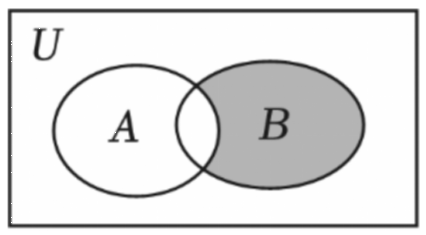
\includegraphics[width=0.26\textwidth]{figures/gao76_q14_venn.png}
\end{center}

\keepwithprev
A. $\{x\mid-2\leqslant x<4\}$\qquad B. $\{x\mid-1\leqslant x\leqslant3\}$

C. $\{x\mid x\leqslant3\text{ 或 }x\geqslant4\}$\qquad D. $\{x\mid-2\leqslant x\leqslant4\}$

\ifanswer
\solbegin
\step{全集 $U=\R$，集合 $A=\{x\mid x<-1\text{ 或 }x>4\}$，}
\step{$B=\{x\mid x^2-x-6\leqslant0\}=\{x\mid-2\leqslant x\leqslant3\}$，故 $A\cap B=\{x\mid-2\leqslant x<-1\}$，}
\step{故阴影部分表示的集合为 $\overline{A\cap B}=\{x\mid-1\leqslant x\leqslant3\}$. 故选 $B$.}
\solend
\fi

\item 设 $a$、$b$、$c\in\R$，给出下列命题：①若 $a>b$，则 $a^2>b^2$，②“$a>b$”是“$a^3>b^3$”的充要条件，③若 $a^2>b^2$，则 $|a|>|b|$，④若 $\dfrac ab>1$，则 $a>b$，⑤若 $a>b$，$c\neq0$，则 $\dfrac a{c^2}>\dfrac b{c^2}$，其中真命题的个数是\mbox{（\quad）}

\keepwithprev
A. $1$ 个\qquad B. $2$ 个\qquad C. $3$ 个\qquad D. $4$ 个

\ifanswer
\solbegin
\step{对于①，取 $a=2$，$b=-2$，满足 $a>b$，而 $a^2=b^2$，故为假命题；}
\step{对于②，$a>b\Leftrightarrow a^3-b^3=(a-b)(a^2+ab+b^2)=(a-b)\left[\left(a+\dfrac12b\right)^2+\dfrac34b^2\right]>0$}
\step{$\Leftrightarrow a^3>b^3$，故为真命题；}
\step{对于③，$a^2>b^2\Leftrightarrow|a|^2>|b|^2\Leftrightarrow|a|>|b|$，故为真命题；}
\step{对于④，取 $a=-2$，$b=-1$，满足 $\dfrac ab>1$，而 $a<b$，故为假命题；}
\step{对于⑤，由题意得 $c^2>0$，由 $a>b$，则 $\dfrac a{c^2}>\dfrac b{c^2}$，故为真命题.}
\step{故选 $C$.}
\solend
\fi

\item 已知关于 $x$ 的两个一元二次不等式 $a_1x^2+b_1x+c_1>0$，$a_2x^2+b_2x+c_2>0$ 的解集分别为 $A$、$B$，其中 $a_i$、$b_i$、$c_i(i=1,2)$ 为常数且不为零，则“$\dfrac{a_1}{a_2}=\dfrac{b_1}{b_2}=\dfrac{c_1}{c_2}$”是“$A=B$”\mbox{（\quad）}

\keepwithprev
A. 充分不必要条件\qquad B. 必要不充分条件

C. 充要条件\qquad D. 既不充分也不必要条件

\ifanswer
\solbegin
\step{设 $\dfrac{a_1}{a_2}=\dfrac{b_1}{b_2}=\dfrac{c_1}{c_2}=\lambda$，}
\step{①当 $\lambda>0$ 时，则 $a_1=\lambda a_2$，$b_1=\lambda b_2$，$c_1=\lambda c_2$，}
\step{$a_1x^2+b_1x+c_1>0\Leftrightarrow\lambda a_2x^2+\lambda b_2x+\lambda c_2>0\Leftrightarrow a_2x^2+b_2x+c_2>0$，}
\step{所以 $A=B$，}
\step{②当 $\lambda<0$ 时，则 $a_1=\lambda a_2$，$b_1=\lambda b_2$，$c_1=\lambda c_2$，}
\step{$a_1x^2+b_1x+c_1>0\Leftrightarrow\lambda a_2x^2+\lambda b_2x+\lambda c_2>0\Leftrightarrow a_2x^2+b_2x+c_2<0$，}
\step{所以 $A\neq B$，充分性不成立，}
\step{当 $A=B=\R$ 时，则 $\Delta<0$ 且 $a_1$、$a_2>0$，$\dfrac{a_1}{a_2}=\dfrac{b_1}{b_2}=\dfrac{c_1}{c_2}$ 不一定成立，}
\step{必要性不成立.}
\step{所以 $\dfrac{a_1}{a_2}=\dfrac{b_1}{b_2}=\dfrac{c_1}{c_2}$ 是 $A=B$ 的既不充分也不必要条件，故选 $D$.}
\solend
\fi

\end{enumerate}

\bigsec{三、解答题}

\begin{enumerate}
\setcounter{enumi}{16}

\item 求下列关于 $x$ 的不等式（组）的解集.

（1）$\begin{cases}9x^2-6x-24>0\\ \dfrac{x+3}{x-1}>2\end{cases}$；

（2）$|2x+1|-|2-x|>2$.

\ifanswer
\solbegin
\stepm{(1)}{不等式 $\dfrac{x+3}{x-1}>2$ 可化为 $\dfrac{x+3}{x-1}-2>0$，}
\step{即 $\dfrac{-x+5}{x-1}>0$，即 $(x-1)(x-5)<0$，解得 $1<x<5$，}
\step{不等式 $9x^2-6x-24>0$ 可化为 $(3x+4)(x-2)>0$，}
\step{解得 $x<-\dfrac43$ 或 $x>2$，}
\step{所以不等式的解集为 $(2,5)$.}
\stepm{(2)}{当 $x\leqslant-\dfrac12$ 时，$|2x+1|-|2-x|>2$ 等价于 $-2x-1-(2-x)>2$，}
\step{解得 $x<-5$，所以 $x<-5$，}
\step{当 $-\dfrac12<x<2$ 时，$|2x+1|-|2-x|>2$ 等价于 $2x+1-(2-x)>2$，}
\step{解得 $x>1$，所以 $1<x<2$，}
\step{当 $x\geqslant2$ 时，$|2x+1|-|2-x|>2$ 等价于 $2x+1-(x-2)>2$，}
\step{解得 $x>-1$，所以 $x\geqslant2$，}
\step{综上，$|2x+1|-|2-x|>2$ 的解集为 $(-\infty,-5)\cup(1,+\infty)$.}
\solend
\fi

\ansspace

\item 设 $m$ 为实数，求关于 $x$ 与 $y$ 的二元一次方程组 $\begin{cases}y=x+m\\ mx-y=4\end{cases}$ 的解集.

\ifanswer
\solbegin
\step{消去 $y$ 得 $(m-1)x=m+4$，}
\step{当 $m-1=0$，即 $m=1$ 时，$0=5$ 不成立，则 $x$ 无解，原方程组的解集为 $\varnothing$；}
\step{当 $m-1\neq0$，即 $m\neq1$ 时，则 $x=\dfrac{m+4}{m-1}$，$y=\dfrac{m+4}{m-1}+m=\dfrac{m^2+4}{m-1}$，}
\step{原方程组的解集为 $\left\{\left(\dfrac{m+4}{m-1},\dfrac{m^2+4}{m-1}\right)\right\}$.}
\step{综上所述，当 $m=1$ 时，方程组的解集为 $\varnothing$；}
\step{当 $m\neq1$ 时，方程组的解集为 $\left\{\left(\dfrac{m+4}{m-1},\dfrac{m^2+4}{m-1}\right)\right\}$.}
\solend
\fi

\ansspace

\item 已知集合 $A=\{x\mid-2\leqslant x-1\leqslant5\}$，集合 $B=\{x\mid m+1\leqslant x\leqslant2m-1\}(m\in\R)$.

（1）若 $m=4$，全集 $U=\R$，求 $A\cap B$；

（2）设命题 $p:x\in A$；命题 $q:x\in B$，若命题 $p$ 是命题 $q$ 的必要不充分条件，求实数 $m$ 的取值范围.

\ifanswer
\solbegin
\stepm{(1)}{由题意得 $A=\{x\mid-2\leqslant x-1\leqslant5\}=\{x\mid-1\leqslant x\leqslant6\}$，}
\step{当 $m=4$ 时，$B=\{x\mid5\leqslant x\leqslant7\}$，$A\cap B=\{x\mid5\leqslant x\leqslant6\}$；}
\stepm{(2)}{因为命题 $p$ 是命题 $q$ 的必要不充分条件，所以集合 $B$ 是集合 $A$ 的真子集，}
\step{当 $B=\varnothing$ 时，$m+1>2m-1$，解得 $m<2$，}
\step{当 $B\neq\varnothing$ 时，$\begin{cases}m+1\leqslant2m-1\\ m+1\geqslant-1\\ 2m-1\leqslant6\end{cases}$（等号不能同时成立），解得 $2\leqslant m\leqslant\dfrac72$，}
\step{综上所述，实数 $m$ 的取值范围为 $\left(-\infty,\dfrac72\right]$.}
\solend
\fi

\ansspace

\item （1）已知实数 $x\neq0$，求 $x+\dfrac1x$ 的取值范围；

（2）如图，要设计一张矩形海报，该海报含有大小相等的左右两个矩形栏目（即图中阴影部分），这两栏的面积之和为 $18000\,\mathrm{cm}^2$，四周空白的宽度为 $10\,\mathrm{cm}$，两栏之间的中缝空白的宽度为 $16\,\mathrm{cm}$，怎样确定海报的高与宽的尺寸（单位：$\mathrm{cm}$），能使矩形海报面积 $S$ 最小？最小面积是多少？

\begin{center}
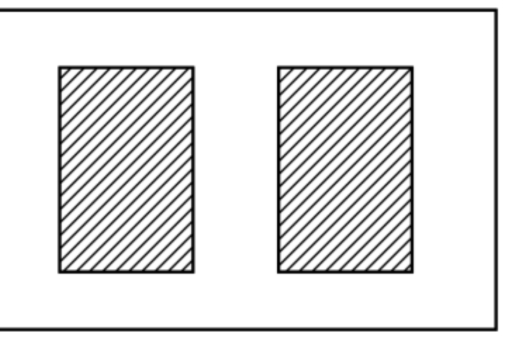
\includegraphics[width=0.34\textwidth]{figures/gao76_q20_poster.png}
\end{center}

\ifanswer
\solbegin
\stepm{(1)}{当 $x>0$ 时，$x+\dfrac1x\geqslant2\sqrt{x\times\dfrac1x}=2$，当且仅当 $x=\dfrac1x$，即 $x=1$ 取等号，}
\step{当 $x<0$ 时，$-x-\dfrac1x\geqslant2\sqrt{(-x)\times\dfrac1{-x}}=2$，所以 $x+\dfrac1x\leqslant-2$，}
\step{当且仅当 $-x=-\dfrac1x$，即 $x=-1$ 取等号，}
\step{综上所述，$x+\dfrac1x$ 的取值范围为 $(-\infty,-2]\cup[2,+\infty)$.}
\stepm{(2)}{设矩形栏目宽为 $x$，高为 $y$，则 $2xy=18000$，}
\step{所以 $S=(2x+36)(y+20)=2xy+36y+40x+720$}
% 原卷此行把 18720 写作 36720，照录（见文件头“原卷笔误/存疑”①）
\step{$=18000+36y+40x+720\geqslant18720+2\sqrt{36y\times40x}$}
\step{$=36720+2\sqrt{36\times40\times18000}=18720+7200=25920$，}
\step{当且仅当 $36y=40x$，即 $x=90$，$y=100$ 取等号，}
\step{所以海报的高为 $120\,\mathrm{cm}$ 与宽为 $216\,\mathrm{cm}$，可使矩形海报面积 $S$ 最小，}
\step{最小面积为 $25920$.}
\solend
\fi

\ansspace

\item 若实数 $x$、$y$、$m$ 满足 $|x-m|>|y-m|$，则称 $x$ 比 $y$ 远离 $m$.

（1）$0$ 比 $\dfrac12$ 远离 $2$ 吗？说明理由；

（2）若 $\dfrac1{2x-1}$ 比 $\dfrac12$ 远离 $1$，求实数 $x$ 的取值范围；

（3）若 $m\leqslant1$，$x+y=2$，试问：$x$ 与 $x^2+y^2$ 哪一个更远离 $m$，并说明理由.

\ifanswer
\solbegin
\stepm{(1)}{$0$ 比 $\dfrac12$ 远离 $2$，理由为：}
\step{由于 $|0-2|=2>\dfrac32=\left|\dfrac12-2\right|$，所以 $0$ 比 $\dfrac12$ 远离 $2$.}
\stepm{(2)}{由 $\dfrac1{2x-1}$ 比 $\dfrac12$ 远离 $1$，得 $\left|\dfrac1{2x-1}-1\right|>\left|\dfrac12-1\right|$，即 $\left|\dfrac1{2x-1}-1\right|>\dfrac12$，}
\step{则 $\dfrac1{2x-1}-1>\dfrac12$ 或 $\dfrac1{2x-1}-1<-\dfrac12$，整理得 $\dfrac1{2x-1}>\dfrac32$ 或 $\dfrac1{2x-1}<\dfrac12$，}
\step{因此 $0<2x-1<\dfrac23$ 或 $2x-1<0$ 或 $2x-1>2$，}
\step{解得 $\dfrac12<x<\dfrac56$ 或 $x<\dfrac12$ 或 $x>\dfrac32$，}
\step{所以 $x$ 的取值范围是 $\left(-\infty,\dfrac12\right)\cup\left(\dfrac12,\dfrac56\right)\cup\left(\dfrac32,+\infty\right)$.}
\stepm{(3)}{$x^2+y^2$ 比 $x$ 更远离 $m$，理由为：}
\step{由 $x^2+y^2\geqslant\dfrac{(x+y)^2}2=2\geqslant m$，得 $|x^2+y^2-m|=x^2+y^2-m$，}
\step{由 $x+y=2$，得 $x^2+y^2=x^2+(2-x)^2=2x^2-4x+4$，}
\step{于是 $|x^2+y^2-m|-|x-m|=2x^2-4x+4-m-|x-m|$，}
\step{当 $x\geqslant m$ 时，$|x^2+y^2-m|-|x-m|=2x^2-4x+4-m-(x-m)$}
\step{$=2\left(x-\dfrac54\right)^2+\dfrac78>0$，即 $|x^2+y^2-m|>|x-m|$；}
\step{当 $x<m$ 时，$|x^2+y^2-m|-|x-m|=2x^2-4x+4-m+(x-m)$}
\step{$=2\left(x-\dfrac34\right)^2+\dfrac{23}8-2m$，}
\step{由 $m\leqslant1$，得 $\dfrac{23}8-2m>0$，因此 $2\left(x-\dfrac34\right)^2+\dfrac{23}8-2m>0$，}
\step{即 $|x^2+y^2-m|>|x-m|$，}
\step{所以 $|x^2+y^2-m|>|x-m|$，即 $x^2+y^2$ 比 $x$ 更远离 $m$.}
\solend
\fi

\ansspace*[7]

\end{enumerate}

\end{document}
"
%
% 原始材料：微信公众号“魔都数学加油站”文章，连载“27学年高一76”；
% 原文标题“27学年高一76——2026-2027年上海市六十中学高一上10月月考”；
% 原文链接：https://mp.weixin.qq.com/s/GrKZjQrV1Xb0wy0BUuzAHw。
% 页面标注发布时间 2026-10-22 21:45（上海）。
% 正文为 10 张 PNG 页（`原图/高一76_六十中学_10月月考/01..10.png`）：
% 第 4、5、8、9 页为 4762×6735，其余 6 页为 2560×3620，均按页序读取。
% 10 页全为试卷正文页（卷首标题在第 1 页页顶，卷末第 21 题 (3) 解析止于第 10 页），
% 无封面页、目录页、二维码或宣传页。粉色斜排“魔都数学加油站”为卷面水印，未录入。
%
% 卷首标题：照卷面印作“2026-2027 年六十中学高一上 10 月月考”（黑体加粗一行）。
% 原卷年份区间用半角连字符，本稿按全稿惯例排 en dash；原卷无副标题。
%
% 篇幅与题号：原卷自第 3 题起编号（第 1、2 题不在本卷内）。填空题 3—12（10 题）、
% 选择题 13—16（4 题）、解答题 17—21（5 题），共 19 题。本稿沿用原节与原题号，
% 只改排为全稿统一的大节样式。
%
% 讲评版：原卷第 3、5 题只印【答案】（“$(0,1)$”“$a$、$b$ 都不能被 $3$ 整除”），
% 本稿只给 \ans{}；其余 17 题均印【解析】，用 \solbegin…\solend。四道选择题的作答
% 括号原卷即留空，答案写在解析末句“故选 C／B／C／D”，照录在解析内，不另提 \ans{}。
%
% 副标题：原卷未印副标题。本稿按“知识模块”口径标作“集合与常用逻辑用语、不等式”：
% 19 题中集合与常用逻辑用语 6 题（第 5、12、14、16、19 题及第 4 题的恒等变形），
% 不等式 13 题（第 3、6—11、13、15、17、18、20、21 题），两类均确有分量，故并标。
% 口径同 高一63、高一68—75。
%
% 与原卷的排版差异：
%   ① 原卷每题下直接印【答案】/【解析】，本稿按全稿惯例将答案与解析置于答案版；
%   ② 原卷未印副标题，本稿按“知识模块”口径补出；
%   ③ 原卷填空横线约四个字宽，本稿按全稿惯例统一排 \blankline[4.4em]；
%   ④ 原卷数集记号排斜体 $R$、$N$（第 4、6、7、8、11、12、14、15、19、20 题），本稿
%      按全稿惯例改用 $\R$、$\N$（同 高一68—75）；第 7、19、20 题的“解集为 $\R$”同此；
%   ⑤ 原卷句末标点多为西文句点，均逐处照录；
%   ⑥ 第 17—21 题的子问原卷印作“（1）…（2）…”，本稿按 高一69—75 成例用行内
%      “（1）（2）（3）”段，解析中的子问标号用 \stepm{(1)}{…}；
%   ⑦ 每道解答题原卷未留作答空白，本稿按全稿惯例加 \ansspace（末题用 \ansspace*）；
%   ⑧ 选择题的作答括号原卷排半角“(    )”，本稿按全稿惯例排 \mbox{（\quad）}；
%      选项行排照原卷——第 13、14、15、16 题一行两条、分两行排（本稿按原卷分行）；
%   ⑨ 第 10、11、17—21 题解析中的不等式组／方程组，原卷均排作“{”连接的多行式，
%      本稿按全稿惯例排 cases；
%   ⑩ 第 14 题题干右侧有一幅韦恩图（全集矩形内含 A、B 两圆，B 涂灰）：本稿按原卷
%      截图裁取（`figures/gao76_q14_venn.png`，由第 5 页原图裁出、去除粉色水印后转
%      灰度，未放大），放在题干之后、选项之前，仅答案版出；
%   ⑪ 第 20 题 (2) 题干右侧有一幅示意图（大矩形内两个斜线阴影小矩形）：本稿按原卷
%      截图裁取（`figures/gao76_q20_poster.png`，由第 8 页原图裁出、去除粉色水印后转
%      灰度，未放大），放在该小题文字之后，仅答案版出。
%
% 原卷笔误/存疑（均照录未改，正文对应处另有 % 注）：
%   ① 第 20 题 (2) 解析第 3 行把 $2xy+720$ 写成 $36720$（实为 $18000+720=18720$），
%      同式下一行又写回 $18720$，前后不一致；原卷如此，照录未改。
%   ② 第 14 题的韦恩图阴影是把整个 $B$ 圆（含 $A\cap B$ 部分）涂灰，而解析按
%      $\overline{A\cap B}$ 求解，二者不一致；原卷图文如此，照录未改。
%
% 行数核对：逐题数 \step/\stepm 条数与原卷【解析】印刷行数，17 题逐一相符，
% 合计 118 条 / 118 行（Q4：3；Q6：4；Q7：1；Q8：6；Q9：3；Q10：7；Q11：4；
% Q12：16；Q13：1；Q14：3；Q15：7；Q16：10；Q17：12；Q18：6；Q19：6；Q20：11；
% Q21：18）。另第 3、5 题只印【答案】，各提 \ans{}，不计入 \step 账。
%
% 插图：第 14 题题干的韦恩图、第 20 题 (2) 的示意图，见上⑩⑪；其余题干无配图。
%
\documentclass[a4paper,11pt]{article}
\usepackage{common}

\begin{document}

\examtitlest[3]{2026--2027 年六十中学高一上 10 月月考}{集合与常用逻辑用语、不等式}

\bigsec{一、填空题}

\begin{enumerate}
\setcounter{enumi}{2}

\item 不等式 $\dfrac{x}{1-x}>0$ 的解集是\blankline[4.4em].

\ifanswer
\ans{$(0,1)$}
\fi

\item 已知 $2x^2+x+1=a(x+1)^2+b(x+1)+2$，对 $x\in\R$ 恒成立，$ab=$\blankline[4.4em].

\ifanswer
\solbegin
\step{若 $2x^2+x+1=a(x+1)^2+b(x+1)+2$ 对 $x\in\R$ 恒成立，}
\step{即 $2x^2+x+1=ax^2+(2a+b)x+a+b+2$ 对 $x\in\R$ 恒成立，}
\step{必有 $\begin{cases}a=2\\ 2a+b=1\\ a+b+2=1\end{cases}$，解得 $a=2$，$b=-3$，所以 $ab=-6$.}
\solend
\fi

\item 利用反证法证明命题：“如果 $a$、$b\in\N$，$ab$ 可被 $3$ 整除，那么 $a$、$b$ 中至少有一个能被 $3$ 整除”时，假设的内容应是\blankline[4.4em].

\ifanswer
\ans{$a$、$b$ 都不能被 $3$ 整除}
\fi

\item 已知 $x\in\R$，方程 $|x+1|+|2-x|=3$ 的解集为\blankline[4.4em].

\ifanswer
\solbegin
\step{当 $x<-1$ 时，则 $|x+1|+|2-x|=-x-1+2-x=1-2x>3$；}
\step{当 $-1\leqslant x\leqslant2$ 时，则 $|x+1|+|2-x|=x+1+2-x=3$；}
\step{当 $x>2$ 时，则 $|x+1|+|2-x|=x+1+x-2=2x-1>3$.}
\step{综上所述，原方程的解集为 $[-1,2]$.}
\solend
\fi

\item 若关于 $x$ 的不等式 $x^2+kx+1\geqslant0$ 的解集为 $\R$，则实数 $k$ 的取值范围是\blankline[4.4em].

\ifanswer
\solbegin
\step{$\Delta=k^2-4\leqslant0\Rightarrow-2\leqslant k\leqslant2$，所以实数 $k$ 的取值范围是 $[-2,2]$.}
\solend
\fi

\item 已知 $a$、$b\in\R$，且 $ab>0$，则下列不等式中，恒成立的序号是\blankline[4.4em].

① $a^2+b^2>2ab$；② $a+b\geqslant2\sqrt{ab}$；③ $\dfrac1a+\dfrac1b>\dfrac2{\sqrt{ab}}$；④ $\dfrac ba+\dfrac ab\geqslant2$.

\ifanswer
\solbegin
\step{因为 $a^2+b^2\geqslant2ab$ 对于 $a$、$b\in\R$ 恒成立，当且仅当 $a=b$ 时取等号，}
\step{所以①错误；}
\step{对于②，③，显然 $a<0$，$b<0$ 时，不等式均不成立，即②和③错误；}
\step{对于④，因为 $ab>0$，所以 $\dfrac ba>0,\dfrac ab>0$，}
\step{由基本不等式得 $\dfrac ba+\dfrac ab\geqslant2\sqrt{\dfrac ba\cdot\dfrac ab}=2$，即④正确.}
\step{故正确的是④.}
\solend
\fi

\item 已知正实数 $m$、$n$ 满足 $m+\dfrac2n=1$，则 $\dfrac1m+2n$ 的最小值为\blankline[4.4em].

\ifanswer
\solbegin
\step{$\dfrac1m+2n=\left(m+\dfrac2n\right)\left(\dfrac1m+2n\right)=5+2mn+\dfrac2{mn}$，}
\step{因为 $mn>0$，所以 $2mn+\dfrac2{mn}\geqslant2\sqrt{2mn\cdot\dfrac2{mn}}=4$，}
\step{当且仅当 $2mn=\dfrac2{mn}$，即 $m=\dfrac13$，$n=3$ 时取等号，所以 $\dfrac1m+2n$ 的最小值为 $9$.}
\solend
\fi

\item 若关于 $x$ 的不等式组 $\begin{cases}3x+1>0\\ x+\dfrac1a\leqslant2\end{cases}$ 恰好有两个整数解，则实数 $a$ 的取值范围为\blankline[4.4em].

\ifanswer
\solbegin
\step{由 $3x+1>0$ 得 $x>-\dfrac13$；若 $a<0$，则 $\dfrac1a<0$，由 $x+\dfrac1a\leqslant2$ 得 $x\leqslant2-\dfrac1a>2$，}
\step{则解集 $\left(-\dfrac13,2-\dfrac1a\right]$ 必同时含有整数 $0$、$1$、$2$，不合题意；}
\step{又 $a=0$ 使 $\dfrac1a$ 无意义，故 $a>0$；}
\step{此时原不等式组的解集为 $\left(-\dfrac13,2-\dfrac1a\right]$，}
\step{其中大于 $-\dfrac13$ 的整数依次为 $0$，$1$，$2$，$\cdots$，}
\step{恰有两个整数解即解集只含 $0$ 与 $1$，故 $1\leqslant2-\dfrac1a<2$，即 $\dfrac1a\leqslant1$ 且 $\dfrac1a>0$，}
\step{结合 $a>0$，解得 $a\geqslant1$.}
\solend
\fi

\item 已知 $a\in\R$，若关于 $x$ 的方程 $x^2+ax+a^2-8=0$ 有两个实根 $x_1$、$x_2$，且 $\dfrac1{x_1}+\dfrac1{x_2}=-\dfrac12$，则 $a$ 的值为\blankline[4.4em].

\ifanswer
\solbegin
\step{由题意得 $\Delta=a^2-4(a^2-8)=32-3a^2\geqslant0$，解得 $a^2\leqslant\dfrac{32}3$，}
\step{由韦达定理得 $x_1+x_2=-a$，$x_1x_2=a^2-8$，}
\step{则 $\dfrac1{x_1}+\dfrac1{x_2}=\dfrac{x_1+x_2}{x_1x_2}=\dfrac{-a}{a^2-8}=-\dfrac12$，即 $a^2-2a-8=(a-4)(a+2)=0$，}
\step{解得 $a=4$ 或 $a=-2$，又 $a^2\leqslant\dfrac{32}3$，则 $a=-2$.}
\solend
\fi

\item 已知有限集 $A=\{a_1,a_2,\cdots,a_n\}(n\geqslant2,n\in\N)$，若 $A$ 中元素 $a_i(i=1,2,\cdots,n)$ 满足 $a_1+a_2+\cdots+a_n=a_1\times a_2\times\cdots\times a_n$，就称 $A$ 为“完美集”，以下四个命题：

①集合 $\{-1-\sqrt3,-1+\sqrt3\}$ 不是“完美集”；

②若 $a_1$、$a_2$ 是两个不同的正数，且 $\{a_1,a_2\}$ 是“完美集”，则 $a_1$、$a_2$ 至少有一个大于 $2$；

③二元“完美集”有无穷多个；

④若 $a_i$ 均为正整数，则“完美集”$A$ 有且只有一个，且 $n=3$.

其中，真命题的序号是\blankline[4.4em].

\ifanswer
\solbegin
\step{对于①选项：$(-1-\sqrt3)+(-1+\sqrt3)=-2$，$(-1-\sqrt3)\times(-1+\sqrt3)=-2$，}
\step{故 $(-1-\sqrt3)+(-1+\sqrt3)=(-1-\sqrt3)\times(-1+\sqrt3)$，}
\step{所以集合 $\{-1-\sqrt3,-1+\sqrt3\}$ 是“完美集”，故①错误；}
\step{对于②选项：集合 $\{a_1,a_2\}$ 是“完美集”，设 $a_1+a_2=a_1a_2=t>0$，}
\step{则 $a_1$、$a_2$ 可以看成一元二次方程 $x^2-tx+t=0$ 的两正根，则 $\Delta=t^2-4t>0$，}
\step{解得 $t<0$（舍）或 $t>4$，即 $a_1a_2>4$，所以至少有一个大于 $2$，故②正确；}
\step{对于③选项：由②得一元二次方程 $x^2-tx+t=0$ 当 $t$ 取不同值时，}
\step{$a_1$、$a_2$ 的值是不同的，因而二元“完美集”有无穷多个，故③正确；}
\step{对于④选项：设 $a_1<a_2<a_3<\cdots<a_n$，}
\step{则 $a_1\times a_2\times\cdots\times a_n=a_1+a_2+\cdots+a_n<na_n$，}
\step{所以 $a_1\times a_2\times\cdots\times a_{n-1}<n$，又 $a_i\in\N^*$，所以 $n\leqslant3$，}
\step{当 $n=2$ 时，$a_1<2$，则 $a_1=1$，$a_1a_2\neq a_1+a_2$，不合题意，}
\step{当 $n=3$ 时，$a_1a_2<3$，所以只能是 $a_1=1$，$a_2=2$，}
\step{由 $a_1+a_2+a_3=a_1a_2a_3$，代入解得 $a_3=3$，所以此时“完美集”只有一个，}
\step{为 $\{1,2,3\}$，故④正确.}
\step{故正确的是②③④.}
\solend
\fi

\end{enumerate}

\bigsec{二、选择题}

\begin{enumerate}
\setcounter{enumi}{12}

\item 已知 $x$、$y\in\R$，则“$xy\geqslant0$”是“$xy=|xy|$”的\mbox{（\quad）}

\keepwithprev
A. 充分非必要条件\qquad B. 必要非充分条件

C. 充要条件\qquad D. 既非充分也非必要条件

\ifanswer
\solbegin
\step{$xy\geqslant0\Leftrightarrow xy=|xy|$，故“$xy\geqslant0$”是“$xy=|xy|$”的充要条件. 故选 $C$.}
\solend
\fi

\needvspace{22\baselineskip}
\item 已知全集 $U=\R$，集合 $A=\{x\mid x<-1\text{ 或 }x>4\}$，$B=\{x\mid x^2-x-6\leqslant0\}$，则阴影部分表示的集合为\mbox{（\quad）}

\begin{center}
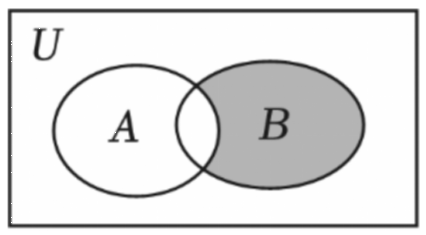
\includegraphics[width=0.26\textwidth]{figures/gao76_q14_venn.png}
\end{center}

\keepwithprev
A. $\{x\mid-2\leqslant x<4\}$\qquad B. $\{x\mid-1\leqslant x\leqslant3\}$

C. $\{x\mid x\leqslant3\text{ 或 }x\geqslant4\}$\qquad D. $\{x\mid-2\leqslant x\leqslant4\}$

\ifanswer
\solbegin
\step{全集 $U=\R$，集合 $A=\{x\mid x<-1\text{ 或 }x>4\}$，}
\step{$B=\{x\mid x^2-x-6\leqslant0\}=\{x\mid-2\leqslant x\leqslant3\}$，故 $A\cap B=\{x\mid-2\leqslant x<-1\}$，}
\step{故阴影部分表示的集合为 $\overline{A\cap B}=\{x\mid-1\leqslant x\leqslant3\}$. 故选 $B$.}
\solend
\fi

\item 设 $a$、$b$、$c\in\R$，给出下列命题：①若 $a>b$，则 $a^2>b^2$，②“$a>b$”是“$a^3>b^3$”的充要条件，③若 $a^2>b^2$，则 $|a|>|b|$，④若 $\dfrac ab>1$，则 $a>b$，⑤若 $a>b$，$c\neq0$，则 $\dfrac a{c^2}>\dfrac b{c^2}$，其中真命题的个数是\mbox{（\quad）}

\keepwithprev
A. $1$ 个\qquad B. $2$ 个\qquad C. $3$ 个\qquad D. $4$ 个

\ifanswer
\solbegin
\step{对于①，取 $a=2$，$b=-2$，满足 $a>b$，而 $a^2=b^2$，故为假命题；}
\step{对于②，$a>b\Leftrightarrow a^3-b^3=(a-b)(a^2+ab+b^2)=(a-b)\left[\left(a+\dfrac12b\right)^2+\dfrac34b^2\right]>0$}
\step{$\Leftrightarrow a^3>b^3$，故为真命题；}
\step{对于③，$a^2>b^2\Leftrightarrow|a|^2>|b|^2\Leftrightarrow|a|>|b|$，故为真命题；}
\step{对于④，取 $a=-2$，$b=-1$，满足 $\dfrac ab>1$，而 $a<b$，故为假命题；}
\step{对于⑤，由题意得 $c^2>0$，由 $a>b$，则 $\dfrac a{c^2}>\dfrac b{c^2}$，故为真命题.}
\step{故选 $C$.}
\solend
\fi

\item 已知关于 $x$ 的两个一元二次不等式 $a_1x^2+b_1x+c_1>0$，$a_2x^2+b_2x+c_2>0$ 的解集分别为 $A$、$B$，其中 $a_i$、$b_i$、$c_i(i=1,2)$ 为常数且不为零，则“$\dfrac{a_1}{a_2}=\dfrac{b_1}{b_2}=\dfrac{c_1}{c_2}$”是“$A=B$”\mbox{（\quad）}

\keepwithprev
A. 充分不必要条件\qquad B. 必要不充分条件

C. 充要条件\qquad D. 既不充分也不必要条件

\ifanswer
\solbegin
\step{设 $\dfrac{a_1}{a_2}=\dfrac{b_1}{b_2}=\dfrac{c_1}{c_2}=\lambda$，}
\step{①当 $\lambda>0$ 时，则 $a_1=\lambda a_2$，$b_1=\lambda b_2$，$c_1=\lambda c_2$，}
\step{$a_1x^2+b_1x+c_1>0\Leftrightarrow\lambda a_2x^2+\lambda b_2x+\lambda c_2>0\Leftrightarrow a_2x^2+b_2x+c_2>0$，}
\step{所以 $A=B$，}
\step{②当 $\lambda<0$ 时，则 $a_1=\lambda a_2$，$b_1=\lambda b_2$，$c_1=\lambda c_2$，}
\step{$a_1x^2+b_1x+c_1>0\Leftrightarrow\lambda a_2x^2+\lambda b_2x+\lambda c_2>0\Leftrightarrow a_2x^2+b_2x+c_2<0$，}
\step{所以 $A\neq B$，充分性不成立，}
\step{当 $A=B=\R$ 时，则 $\Delta<0$ 且 $a_1$、$a_2>0$，$\dfrac{a_1}{a_2}=\dfrac{b_1}{b_2}=\dfrac{c_1}{c_2}$ 不一定成立，}
\step{必要性不成立.}
\step{所以 $\dfrac{a_1}{a_2}=\dfrac{b_1}{b_2}=\dfrac{c_1}{c_2}$ 是 $A=B$ 的既不充分也不必要条件，故选 $D$.}
\solend
\fi

\end{enumerate}

\bigsec{三、解答题}

\begin{enumerate}
\setcounter{enumi}{16}

\item 求下列关于 $x$ 的不等式（组）的解集.

（1）$\begin{cases}9x^2-6x-24>0\\ \dfrac{x+3}{x-1}>2\end{cases}$；

（2）$|2x+1|-|2-x|>2$.

\ifanswer
\solbegin
\stepm{(1)}{不等式 $\dfrac{x+3}{x-1}>2$ 可化为 $\dfrac{x+3}{x-1}-2>0$，}
\step{即 $\dfrac{-x+5}{x-1}>0$，即 $(x-1)(x-5)<0$，解得 $1<x<5$，}
\step{不等式 $9x^2-6x-24>0$ 可化为 $(3x+4)(x-2)>0$，}
\step{解得 $x<-\dfrac43$ 或 $x>2$，}
\step{所以不等式的解集为 $(2,5)$.}
\stepm{(2)}{当 $x\leqslant-\dfrac12$ 时，$|2x+1|-|2-x|>2$ 等价于 $-2x-1-(2-x)>2$，}
\step{解得 $x<-5$，所以 $x<-5$，}
\step{当 $-\dfrac12<x<2$ 时，$|2x+1|-|2-x|>2$ 等价于 $2x+1-(2-x)>2$，}
\step{解得 $x>1$，所以 $1<x<2$，}
\step{当 $x\geqslant2$ 时，$|2x+1|-|2-x|>2$ 等价于 $2x+1-(x-2)>2$，}
\step{解得 $x>-1$，所以 $x\geqslant2$，}
\step{综上，$|2x+1|-|2-x|>2$ 的解集为 $(-\infty,-5)\cup(1,+\infty)$.}
\solend
\fi

\ansspace

\item 设 $m$ 为实数，求关于 $x$ 与 $y$ 的二元一次方程组 $\begin{cases}y=x+m\\ mx-y=4\end{cases}$ 的解集.

\ifanswer
\solbegin
\step{消去 $y$ 得 $(m-1)x=m+4$，}
\step{当 $m-1=0$，即 $m=1$ 时，$0=5$ 不成立，则 $x$ 无解，原方程组的解集为 $\varnothing$；}
\step{当 $m-1\neq0$，即 $m\neq1$ 时，则 $x=\dfrac{m+4}{m-1}$，$y=\dfrac{m+4}{m-1}+m=\dfrac{m^2+4}{m-1}$，}
\step{原方程组的解集为 $\left\{\left(\dfrac{m+4}{m-1},\dfrac{m^2+4}{m-1}\right)\right\}$.}
\step{综上所述，当 $m=1$ 时，方程组的解集为 $\varnothing$；}
\step{当 $m\neq1$ 时，方程组的解集为 $\left\{\left(\dfrac{m+4}{m-1},\dfrac{m^2+4}{m-1}\right)\right\}$.}
\solend
\fi

\ansspace

\item 已知集合 $A=\{x\mid-2\leqslant x-1\leqslant5\}$，集合 $B=\{x\mid m+1\leqslant x\leqslant2m-1\}(m\in\R)$.

（1）若 $m=4$，全集 $U=\R$，求 $A\cap B$；

（2）设命题 $p:x\in A$；命题 $q:x\in B$，若命题 $p$ 是命题 $q$ 的必要不充分条件，求实数 $m$ 的取值范围.

\ifanswer
\solbegin
\stepm{(1)}{由题意得 $A=\{x\mid-2\leqslant x-1\leqslant5\}=\{x\mid-1\leqslant x\leqslant6\}$，}
\step{当 $m=4$ 时，$B=\{x\mid5\leqslant x\leqslant7\}$，$A\cap B=\{x\mid5\leqslant x\leqslant6\}$；}
\stepm{(2)}{因为命题 $p$ 是命题 $q$ 的必要不充分条件，所以集合 $B$ 是集合 $A$ 的真子集，}
\step{当 $B=\varnothing$ 时，$m+1>2m-1$，解得 $m<2$，}
\step{当 $B\neq\varnothing$ 时，$\begin{cases}m+1\leqslant2m-1\\ m+1\geqslant-1\\ 2m-1\leqslant6\end{cases}$（等号不能同时成立），解得 $2\leqslant m\leqslant\dfrac72$，}
\step{综上所述，实数 $m$ 的取值范围为 $\left(-\infty,\dfrac72\right]$.}
\solend
\fi

\ansspace

\item （1）已知实数 $x\neq0$，求 $x+\dfrac1x$ 的取值范围；

（2）如图，要设计一张矩形海报，该海报含有大小相等的左右两个矩形栏目（即图中阴影部分），这两栏的面积之和为 $18000\,\mathrm{cm}^2$，四周空白的宽度为 $10\,\mathrm{cm}$，两栏之间的中缝空白的宽度为 $16\,\mathrm{cm}$，怎样确定海报的高与宽的尺寸（单位：$\mathrm{cm}$），能使矩形海报面积 $S$ 最小？最小面积是多少？

\begin{center}
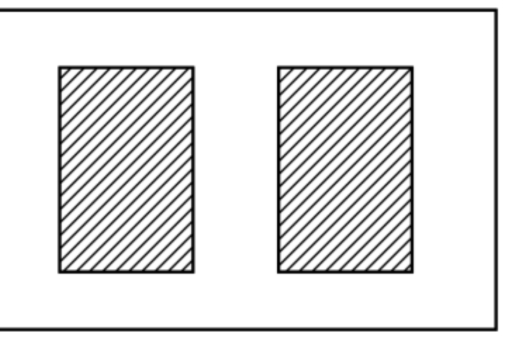
\includegraphics[width=0.34\textwidth]{figures/gao76_q20_poster.png}
\end{center}

\ifanswer
\solbegin
\stepm{(1)}{当 $x>0$ 时，$x+\dfrac1x\geqslant2\sqrt{x\times\dfrac1x}=2$，当且仅当 $x=\dfrac1x$，即 $x=1$ 取等号，}
\step{当 $x<0$ 时，$-x-\dfrac1x\geqslant2\sqrt{(-x)\times\dfrac1{-x}}=2$，所以 $x+\dfrac1x\leqslant-2$，}
\step{当且仅当 $-x=-\dfrac1x$，即 $x=-1$ 取等号，}
\step{综上所述，$x+\dfrac1x$ 的取值范围为 $(-\infty,-2]\cup[2,+\infty)$.}
\stepm{(2)}{设矩形栏目宽为 $x$，高为 $y$，则 $2xy=18000$，}
\step{所以 $S=(2x+36)(y+20)=2xy+36y+40x+720$}
% 原卷此行把 18720 写作 36720，照录（见文件头“原卷笔误/存疑”①）
\step{$=18000+36y+40x+720\geqslant18720+2\sqrt{36y\times40x}$}
\step{$=36720+2\sqrt{36\times40\times18000}=18720+7200=25920$，}
\step{当且仅当 $36y=40x$，即 $x=90$，$y=100$ 取等号，}
\step{所以海报的高为 $120\,\mathrm{cm}$ 与宽为 $216\,\mathrm{cm}$，可使矩形海报面积 $S$ 最小，}
\step{最小面积为 $25920$.}
\solend
\fi

\ansspace

\item 若实数 $x$、$y$、$m$ 满足 $|x-m|>|y-m|$，则称 $x$ 比 $y$ 远离 $m$.

（1）$0$ 比 $\dfrac12$ 远离 $2$ 吗？说明理由；

（2）若 $\dfrac1{2x-1}$ 比 $\dfrac12$ 远离 $1$，求实数 $x$ 的取值范围；

（3）若 $m\leqslant1$，$x+y=2$，试问：$x$ 与 $x^2+y^2$ 哪一个更远离 $m$，并说明理由.

\ifanswer
\solbegin
\stepm{(1)}{$0$ 比 $\dfrac12$ 远离 $2$，理由为：}
\step{由于 $|0-2|=2>\dfrac32=\left|\dfrac12-2\right|$，所以 $0$ 比 $\dfrac12$ 远离 $2$.}
\stepm{(2)}{由 $\dfrac1{2x-1}$ 比 $\dfrac12$ 远离 $1$，得 $\left|\dfrac1{2x-1}-1\right|>\left|\dfrac12-1\right|$，即 $\left|\dfrac1{2x-1}-1\right|>\dfrac12$，}
\step{则 $\dfrac1{2x-1}-1>\dfrac12$ 或 $\dfrac1{2x-1}-1<-\dfrac12$，整理得 $\dfrac1{2x-1}>\dfrac32$ 或 $\dfrac1{2x-1}<\dfrac12$，}
\step{因此 $0<2x-1<\dfrac23$ 或 $2x-1<0$ 或 $2x-1>2$，}
\step{解得 $\dfrac12<x<\dfrac56$ 或 $x<\dfrac12$ 或 $x>\dfrac32$，}
\step{所以 $x$ 的取值范围是 $\left(-\infty,\dfrac12\right)\cup\left(\dfrac12,\dfrac56\right)\cup\left(\dfrac32,+\infty\right)$.}
\stepm{(3)}{$x^2+y^2$ 比 $x$ 更远离 $m$，理由为：}
\step{由 $x^2+y^2\geqslant\dfrac{(x+y)^2}2=2\geqslant m$，得 $|x^2+y^2-m|=x^2+y^2-m$，}
\step{由 $x+y=2$，得 $x^2+y^2=x^2+(2-x)^2=2x^2-4x+4$，}
\step{于是 $|x^2+y^2-m|-|x-m|=2x^2-4x+4-m-|x-m|$，}
\step{当 $x\geqslant m$ 时，$|x^2+y^2-m|-|x-m|=2x^2-4x+4-m-(x-m)$}
\step{$=2\left(x-\dfrac54\right)^2+\dfrac78>0$，即 $|x^2+y^2-m|>|x-m|$；}
\step{当 $x<m$ 时，$|x^2+y^2-m|-|x-m|=2x^2-4x+4-m+(x-m)$}
\step{$=2\left(x-\dfrac34\right)^2+\dfrac{23}8-2m$，}
\step{由 $m\leqslant1$，得 $\dfrac{23}8-2m>0$，因此 $2\left(x-\dfrac34\right)^2+\dfrac{23}8-2m>0$，}
\step{即 $|x^2+y^2-m|>|x-m|$，}
\step{所以 $|x^2+y^2-m|>|x-m|$，即 $x^2+y^2$ 比 $x$ 更远离 $m$.}
\solend
\fi

\ansspace*[7]

\end{enumerate}

\end{document}
"
%
% 原始材料：微信公众号“魔都数学加油站”文章，连载“27学年高一76”；
% 原文标题“27学年高一76——2026-2027年上海市六十中学高一上10月月考”；
% 原文链接：https://mp.weixin.qq.com/s/GrKZjQrV1Xb0wy0BUuzAHw。
% 页面标注发布时间 2026-10-22 21:45（上海）。
% 正文为 10 张 PNG 页（`原图/高一76_六十中学_10月月考/01..10.png`）：
% 第 4、5、8、9 页为 4762×6735，其余 6 页为 2560×3620，均按页序读取。
% 10 页全为试卷正文页（卷首标题在第 1 页页顶，卷末第 21 题 (3) 解析止于第 10 页），
% 无封面页、目录页、二维码或宣传页。粉色斜排“魔都数学加油站”为卷面水印，未录入。
%
% 卷首标题：照卷面印作“2026-2027 年六十中学高一上 10 月月考”（黑体加粗一行）。
% 原卷年份区间用半角连字符，本稿按全稿惯例排 en dash；原卷无副标题。
%
% 篇幅与题号：原卷自第 3 题起编号（第 1、2 题不在本卷内）。填空题 3—12（10 题）、
% 选择题 13—16（4 题）、解答题 17—21（5 题），共 19 题。本稿沿用原节与原题号，
% 只改排为全稿统一的大节样式。
%
% 讲评版：原卷第 3、5 题只印【答案】（“$(0,1)$”“$a$、$b$ 都不能被 $3$ 整除”），
% 本稿只给 \ans{}；其余 17 题均印【解析】，用 \solbegin…\solend。四道选择题的作答
% 括号原卷即留空，答案写在解析末句“故选 C／B／C／D”，照录在解析内，不另提 \ans{}。
%
% 副标题：原卷未印副标题。本稿按“知识模块”口径标作“集合与常用逻辑用语、不等式”：
% 19 题中集合与常用逻辑用语 6 题（第 5、12、14、16、19 题及第 4 题的恒等变形），
% 不等式 13 题（第 3、6—11、13、15、17、18、20、21 题），两类均确有分量，故并标。
% 口径同 高一63、高一68—75。
%
% 与原卷的排版差异：
%   ① 原卷每题下直接印【答案】/【解析】，本稿按全稿惯例将答案与解析置于答案版；
%   ② 原卷未印副标题，本稿按“知识模块”口径补出；
%   ③ 原卷填空横线约四个字宽，本稿按全稿惯例统一排 \blankline[4.4em]；
%   ④ 原卷数集记号排斜体 $R$、$N$（第 4、6、7、8、11、12、14、15、19、20 题），本稿
%      按全稿惯例改用 $\R$、$\N$（同 高一68—75）；第 7、19、20 题的“解集为 $\R$”同此；
%   ⑤ 原卷句末标点多为西文句点，均逐处照录；
%   ⑥ 第 17—21 题的子问原卷印作“（1）…（2）…”，本稿按 高一69—75 成例用行内
%      “（1）（2）（3）”段，解析中的子问标号用 \stepm{(1)}{…}；
%   ⑦ 每道解答题原卷未留作答空白，本稿按全稿惯例加 \ansspace（末题用 \ansspace*）；
%   ⑧ 选择题的作答括号原卷排半角“(    )”，本稿按全稿惯例排 \mbox{（\quad）}；
%      选项行排照原卷——第 13、14、15、16 题一行两条、分两行排（本稿按原卷分行）；
%   ⑨ 第 10、11、17—21 题解析中的不等式组／方程组，原卷均排作“{”连接的多行式，
%      本稿按全稿惯例排 cases；
%   ⑩ 第 14 题题干右侧有一幅韦恩图（全集矩形内含 A、B 两圆，B 涂灰）：本稿按原卷
%      截图裁取（`figures/gao76_q14_venn.png`，由第 5 页原图裁出、去除粉色水印后转
%      灰度，未放大），放在题干之后、选项之前，仅答案版出；
%   ⑪ 第 20 题 (2) 题干右侧有一幅示意图（大矩形内两个斜线阴影小矩形）：本稿按原卷
%      截图裁取（`figures/gao76_q20_poster.png`，由第 8 页原图裁出、去除粉色水印后转
%      灰度，未放大），放在该小题文字之后，仅答案版出。
%
% 原卷笔误/存疑（均照录未改，正文对应处另有 % 注）：
%   ① 第 20 题 (2) 解析第 3 行把 $2xy+720$ 写成 $36720$（实为 $18000+720=18720$），
%      同式下一行又写回 $18720$，前后不一致；原卷如此，照录未改。
%   ② 第 14 题的韦恩图阴影是把整个 $B$ 圆（含 $A\cap B$ 部分）涂灰，而解析按
%      $\overline{A\cap B}$ 求解，二者不一致；原卷图文如此，照录未改。
%
% 行数核对：逐题数 \step/\stepm 条数与原卷【解析】印刷行数，17 题逐一相符，
% 合计 118 条 / 118 行（Q4：3；Q6：4；Q7：1；Q8：6；Q9：3；Q10：7；Q11：4；
% Q12：16；Q13：1；Q14：3；Q15：7；Q16：10；Q17：12；Q18：6；Q19：6；Q20：11；
% Q21：18）。另第 3、5 题只印【答案】，各提 \ans{}，不计入 \step 账。
%
% 插图：第 14 题题干的韦恩图、第 20 题 (2) 的示意图，见上⑩⑪；其余题干无配图。
%
\documentclass[a4paper,11pt]{article}
\usepackage{common}

\begin{document}

\examtitlest[3]{2026--2027 年六十中学高一上 10 月月考}{集合与常用逻辑用语、不等式}

\bigsec{一、填空题}

\begin{enumerate}
\setcounter{enumi}{2}

\item 不等式 $\dfrac{x}{1-x}>0$ 的解集是\blankline[4.4em].

\ifanswer
\ans{$(0,1)$}
\fi

\item 已知 $2x^2+x+1=a(x+1)^2+b(x+1)+2$，对 $x\in\R$ 恒成立，$ab=$\blankline[4.4em].

\ifanswer
\solbegin
\step{若 $2x^2+x+1=a(x+1)^2+b(x+1)+2$ 对 $x\in\R$ 恒成立，}
\step{即 $2x^2+x+1=ax^2+(2a+b)x+a+b+2$ 对 $x\in\R$ 恒成立，}
\step{必有 $\begin{cases}a=2\\ 2a+b=1\\ a+b+2=1\end{cases}$，解得 $a=2$，$b=-3$，所以 $ab=-6$.}
\solend
\fi

\item 利用反证法证明命题：“如果 $a$、$b\in\N$，$ab$ 可被 $3$ 整除，那么 $a$、$b$ 中至少有一个能被 $3$ 整除”时，假设的内容应是\blankline[4.4em].

\ifanswer
\ans{$a$、$b$ 都不能被 $3$ 整除}
\fi

\item 已知 $x\in\R$，方程 $|x+1|+|2-x|=3$ 的解集为\blankline[4.4em].

\ifanswer
\solbegin
\step{当 $x<-1$ 时，则 $|x+1|+|2-x|=-x-1+2-x=1-2x>3$；}
\step{当 $-1\leqslant x\leqslant2$ 时，则 $|x+1|+|2-x|=x+1+2-x=3$；}
\step{当 $x>2$ 时，则 $|x+1|+|2-x|=x+1+x-2=2x-1>3$.}
\step{综上所述，原方程的解集为 $[-1,2]$.}
\solend
\fi

\item 若关于 $x$ 的不等式 $x^2+kx+1\geqslant0$ 的解集为 $\R$，则实数 $k$ 的取值范围是\blankline[4.4em].

\ifanswer
\solbegin
\step{$\Delta=k^2-4\leqslant0\Rightarrow-2\leqslant k\leqslant2$，所以实数 $k$ 的取值范围是 $[-2,2]$.}
\solend
\fi

\item 已知 $a$、$b\in\R$，且 $ab>0$，则下列不等式中，恒成立的序号是\blankline[4.4em].

① $a^2+b^2>2ab$；② $a+b\geqslant2\sqrt{ab}$；③ $\dfrac1a+\dfrac1b>\dfrac2{\sqrt{ab}}$；④ $\dfrac ba+\dfrac ab\geqslant2$.

\ifanswer
\solbegin
\step{因为 $a^2+b^2\geqslant2ab$ 对于 $a$、$b\in\R$ 恒成立，当且仅当 $a=b$ 时取等号，}
\step{所以①错误；}
\step{对于②，③，显然 $a<0$，$b<0$ 时，不等式均不成立，即②和③错误；}
\step{对于④，因为 $ab>0$，所以 $\dfrac ba>0,\dfrac ab>0$，}
\step{由基本不等式得 $\dfrac ba+\dfrac ab\geqslant2\sqrt{\dfrac ba\cdot\dfrac ab}=2$，即④正确.}
\step{故正确的是④.}
\solend
\fi

\item 已知正实数 $m$、$n$ 满足 $m+\dfrac2n=1$，则 $\dfrac1m+2n$ 的最小值为\blankline[4.4em].

\ifanswer
\solbegin
\step{$\dfrac1m+2n=\left(m+\dfrac2n\right)\left(\dfrac1m+2n\right)=5+2mn+\dfrac2{mn}$，}
\step{因为 $mn>0$，所以 $2mn+\dfrac2{mn}\geqslant2\sqrt{2mn\cdot\dfrac2{mn}}=4$，}
\step{当且仅当 $2mn=\dfrac2{mn}$，即 $m=\dfrac13$，$n=3$ 时取等号，所以 $\dfrac1m+2n$ 的最小值为 $9$.}
\solend
\fi

\item 若关于 $x$ 的不等式组 $\begin{cases}3x+1>0\\ x+\dfrac1a\leqslant2\end{cases}$ 恰好有两个整数解，则实数 $a$ 的取值范围为\blankline[4.4em].

\ifanswer
\solbegin
\step{由 $3x+1>0$ 得 $x>-\dfrac13$；若 $a<0$，则 $\dfrac1a<0$，由 $x+\dfrac1a\leqslant2$ 得 $x\leqslant2-\dfrac1a>2$，}
\step{则解集 $\left(-\dfrac13,2-\dfrac1a\right]$ 必同时含有整数 $0$、$1$、$2$，不合题意；}
\step{又 $a=0$ 使 $\dfrac1a$ 无意义，故 $a>0$；}
\step{此时原不等式组的解集为 $\left(-\dfrac13,2-\dfrac1a\right]$，}
\step{其中大于 $-\dfrac13$ 的整数依次为 $0$，$1$，$2$，$\cdots$，}
\step{恰有两个整数解即解集只含 $0$ 与 $1$，故 $1\leqslant2-\dfrac1a<2$，即 $\dfrac1a\leqslant1$ 且 $\dfrac1a>0$，}
\step{结合 $a>0$，解得 $a\geqslant1$.}
\solend
\fi

\item 已知 $a\in\R$，若关于 $x$ 的方程 $x^2+ax+a^2-8=0$ 有两个实根 $x_1$、$x_2$，且 $\dfrac1{x_1}+\dfrac1{x_2}=-\dfrac12$，则 $a$ 的值为\blankline[4.4em].

\ifanswer
\solbegin
\step{由题意得 $\Delta=a^2-4(a^2-8)=32-3a^2\geqslant0$，解得 $a^2\leqslant\dfrac{32}3$，}
\step{由韦达定理得 $x_1+x_2=-a$，$x_1x_2=a^2-8$，}
\step{则 $\dfrac1{x_1}+\dfrac1{x_2}=\dfrac{x_1+x_2}{x_1x_2}=\dfrac{-a}{a^2-8}=-\dfrac12$，即 $a^2-2a-8=(a-4)(a+2)=0$，}
\step{解得 $a=4$ 或 $a=-2$，又 $a^2\leqslant\dfrac{32}3$，则 $a=-2$.}
\solend
\fi

\item 已知有限集 $A=\{a_1,a_2,\cdots,a_n\}(n\geqslant2,n\in\N)$，若 $A$ 中元素 $a_i(i=1,2,\cdots,n)$ 满足 $a_1+a_2+\cdots+a_n=a_1\times a_2\times\cdots\times a_n$，就称 $A$ 为“完美集”，以下四个命题：

①集合 $\{-1-\sqrt3,-1+\sqrt3\}$ 不是“完美集”；

②若 $a_1$、$a_2$ 是两个不同的正数，且 $\{a_1,a_2\}$ 是“完美集”，则 $a_1$、$a_2$ 至少有一个大于 $2$；

③二元“完美集”有无穷多个；

④若 $a_i$ 均为正整数，则“完美集”$A$ 有且只有一个，且 $n=3$.

其中，真命题的序号是\blankline[4.4em].

\ifanswer
\solbegin
\step{对于①选项：$(-1-\sqrt3)+(-1+\sqrt3)=-2$，$(-1-\sqrt3)\times(-1+\sqrt3)=-2$，}
\step{故 $(-1-\sqrt3)+(-1+\sqrt3)=(-1-\sqrt3)\times(-1+\sqrt3)$，}
\step{所以集合 $\{-1-\sqrt3,-1+\sqrt3\}$ 是“完美集”，故①错误；}
\step{对于②选项：集合 $\{a_1,a_2\}$ 是“完美集”，设 $a_1+a_2=a_1a_2=t>0$，}
\step{则 $a_1$、$a_2$ 可以看成一元二次方程 $x^2-tx+t=0$ 的两正根，则 $\Delta=t^2-4t>0$，}
\step{解得 $t<0$（舍）或 $t>4$，即 $a_1a_2>4$，所以至少有一个大于 $2$，故②正确；}
\step{对于③选项：由②得一元二次方程 $x^2-tx+t=0$ 当 $t$ 取不同值时，}
\step{$a_1$、$a_2$ 的值是不同的，因而二元“完美集”有无穷多个，故③正确；}
\step{对于④选项：设 $a_1<a_2<a_3<\cdots<a_n$，}
\step{则 $a_1\times a_2\times\cdots\times a_n=a_1+a_2+\cdots+a_n<na_n$，}
\step{所以 $a_1\times a_2\times\cdots\times a_{n-1}<n$，又 $a_i\in\N^*$，所以 $n\leqslant3$，}
\step{当 $n=2$ 时，$a_1<2$，则 $a_1=1$，$a_1a_2\neq a_1+a_2$，不合题意，}
\step{当 $n=3$ 时，$a_1a_2<3$，所以只能是 $a_1=1$，$a_2=2$，}
\step{由 $a_1+a_2+a_3=a_1a_2a_3$，代入解得 $a_3=3$，所以此时“完美集”只有一个，}
\step{为 $\{1,2,3\}$，故④正确.}
\step{故正确的是②③④.}
\solend
\fi

\end{enumerate}

\bigsec{二、选择题}

\begin{enumerate}
\setcounter{enumi}{12}

\item 已知 $x$、$y\in\R$，则“$xy\geqslant0$”是“$xy=|xy|$”的\mbox{（\quad）}

\keepwithprev
A. 充分非必要条件\qquad B. 必要非充分条件

C. 充要条件\qquad D. 既非充分也非必要条件

\ifanswer
\solbegin
\step{$xy\geqslant0\Leftrightarrow xy=|xy|$，故“$xy\geqslant0$”是“$xy=|xy|$”的充要条件. 故选 $C$.}
\solend
\fi

\needvspace{22\baselineskip}
\item 已知全集 $U=\R$，集合 $A=\{x\mid x<-1\text{ 或 }x>4\}$，$B=\{x\mid x^2-x-6\leqslant0\}$，则阴影部分表示的集合为\mbox{（\quad）}

\begin{center}
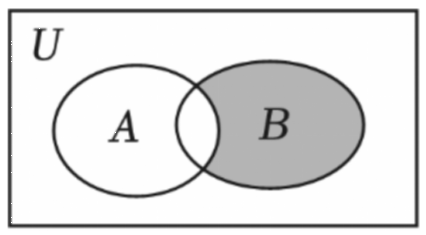
\includegraphics[width=0.26\textwidth]{figures/gao76_q14_venn.png}
\end{center}

\keepwithprev
A. $\{x\mid-2\leqslant x<4\}$\qquad B. $\{x\mid-1\leqslant x\leqslant3\}$

C. $\{x\mid x\leqslant3\text{ 或 }x\geqslant4\}$\qquad D. $\{x\mid-2\leqslant x\leqslant4\}$

\ifanswer
\solbegin
\step{全集 $U=\R$，集合 $A=\{x\mid x<-1\text{ 或 }x>4\}$，}
\step{$B=\{x\mid x^2-x-6\leqslant0\}=\{x\mid-2\leqslant x\leqslant3\}$，故 $A\cap B=\{x\mid-2\leqslant x<-1\}$，}
\step{故阴影部分表示的集合为 $\overline{A\cap B}=\{x\mid-1\leqslant x\leqslant3\}$. 故选 $B$.}
\solend
\fi

\item 设 $a$、$b$、$c\in\R$，给出下列命题：①若 $a>b$，则 $a^2>b^2$，②“$a>b$”是“$a^3>b^3$”的充要条件，③若 $a^2>b^2$，则 $|a|>|b|$，④若 $\dfrac ab>1$，则 $a>b$，⑤若 $a>b$，$c\neq0$，则 $\dfrac a{c^2}>\dfrac b{c^2}$，其中真命题的个数是\mbox{（\quad）}

\keepwithprev
A. $1$ 个\qquad B. $2$ 个\qquad C. $3$ 个\qquad D. $4$ 个

\ifanswer
\solbegin
\step{对于①，取 $a=2$，$b=-2$，满足 $a>b$，而 $a^2=b^2$，故为假命题；}
\step{对于②，$a>b\Leftrightarrow a^3-b^3=(a-b)(a^2+ab+b^2)=(a-b)\left[\left(a+\dfrac12b\right)^2+\dfrac34b^2\right]>0$}
\step{$\Leftrightarrow a^3>b^3$，故为真命题；}
\step{对于③，$a^2>b^2\Leftrightarrow|a|^2>|b|^2\Leftrightarrow|a|>|b|$，故为真命题；}
\step{对于④，取 $a=-2$，$b=-1$，满足 $\dfrac ab>1$，而 $a<b$，故为假命题；}
\step{对于⑤，由题意得 $c^2>0$，由 $a>b$，则 $\dfrac a{c^2}>\dfrac b{c^2}$，故为真命题.}
\step{故选 $C$.}
\solend
\fi

\item 已知关于 $x$ 的两个一元二次不等式 $a_1x^2+b_1x+c_1>0$，$a_2x^2+b_2x+c_2>0$ 的解集分别为 $A$、$B$，其中 $a_i$、$b_i$、$c_i(i=1,2)$ 为常数且不为零，则“$\dfrac{a_1}{a_2}=\dfrac{b_1}{b_2}=\dfrac{c_1}{c_2}$”是“$A=B$”\mbox{（\quad）}

\keepwithprev
A. 充分不必要条件\qquad B. 必要不充分条件

C. 充要条件\qquad D. 既不充分也不必要条件

\ifanswer
\solbegin
\step{设 $\dfrac{a_1}{a_2}=\dfrac{b_1}{b_2}=\dfrac{c_1}{c_2}=\lambda$，}
\step{①当 $\lambda>0$ 时，则 $a_1=\lambda a_2$，$b_1=\lambda b_2$，$c_1=\lambda c_2$，}
\step{$a_1x^2+b_1x+c_1>0\Leftrightarrow\lambda a_2x^2+\lambda b_2x+\lambda c_2>0\Leftrightarrow a_2x^2+b_2x+c_2>0$，}
\step{所以 $A=B$，}
\step{②当 $\lambda<0$ 时，则 $a_1=\lambda a_2$，$b_1=\lambda b_2$，$c_1=\lambda c_2$，}
\step{$a_1x^2+b_1x+c_1>0\Leftrightarrow\lambda a_2x^2+\lambda b_2x+\lambda c_2>0\Leftrightarrow a_2x^2+b_2x+c_2<0$，}
\step{所以 $A\neq B$，充分性不成立，}
\step{当 $A=B=\R$ 时，则 $\Delta<0$ 且 $a_1$、$a_2>0$，$\dfrac{a_1}{a_2}=\dfrac{b_1}{b_2}=\dfrac{c_1}{c_2}$ 不一定成立，}
\step{必要性不成立.}
\step{所以 $\dfrac{a_1}{a_2}=\dfrac{b_1}{b_2}=\dfrac{c_1}{c_2}$ 是 $A=B$ 的既不充分也不必要条件，故选 $D$.}
\solend
\fi

\end{enumerate}

\bigsec{三、解答题}

\begin{enumerate}
\setcounter{enumi}{16}

\item 求下列关于 $x$ 的不等式（组）的解集.

（1）$\begin{cases}9x^2-6x-24>0\\ \dfrac{x+3}{x-1}>2\end{cases}$；

（2）$|2x+1|-|2-x|>2$.

\ifanswer
\solbegin
\stepm{(1)}{不等式 $\dfrac{x+3}{x-1}>2$ 可化为 $\dfrac{x+3}{x-1}-2>0$，}
\step{即 $\dfrac{-x+5}{x-1}>0$，即 $(x-1)(x-5)<0$，解得 $1<x<5$，}
\step{不等式 $9x^2-6x-24>0$ 可化为 $(3x+4)(x-2)>0$，}
\step{解得 $x<-\dfrac43$ 或 $x>2$，}
\step{所以不等式的解集为 $(2,5)$.}
\stepm{(2)}{当 $x\leqslant-\dfrac12$ 时，$|2x+1|-|2-x|>2$ 等价于 $-2x-1-(2-x)>2$，}
\step{解得 $x<-5$，所以 $x<-5$，}
\step{当 $-\dfrac12<x<2$ 时，$|2x+1|-|2-x|>2$ 等价于 $2x+1-(2-x)>2$，}
\step{解得 $x>1$，所以 $1<x<2$，}
\step{当 $x\geqslant2$ 时，$|2x+1|-|2-x|>2$ 等价于 $2x+1-(x-2)>2$，}
\step{解得 $x>-1$，所以 $x\geqslant2$，}
\step{综上，$|2x+1|-|2-x|>2$ 的解集为 $(-\infty,-5)\cup(1,+\infty)$.}
\solend
\fi

\ansspace

\item 设 $m$ 为实数，求关于 $x$ 与 $y$ 的二元一次方程组 $\begin{cases}y=x+m\\ mx-y=4\end{cases}$ 的解集.

\ifanswer
\solbegin
\step{消去 $y$ 得 $(m-1)x=m+4$，}
\step{当 $m-1=0$，即 $m=1$ 时，$0=5$ 不成立，则 $x$ 无解，原方程组的解集为 $\varnothing$；}
\step{当 $m-1\neq0$，即 $m\neq1$ 时，则 $x=\dfrac{m+4}{m-1}$，$y=\dfrac{m+4}{m-1}+m=\dfrac{m^2+4}{m-1}$，}
\step{原方程组的解集为 $\left\{\left(\dfrac{m+4}{m-1},\dfrac{m^2+4}{m-1}\right)\right\}$.}
\step{综上所述，当 $m=1$ 时，方程组的解集为 $\varnothing$；}
\step{当 $m\neq1$ 时，方程组的解集为 $\left\{\left(\dfrac{m+4}{m-1},\dfrac{m^2+4}{m-1}\right)\right\}$.}
\solend
\fi

\ansspace

\item 已知集合 $A=\{x\mid-2\leqslant x-1\leqslant5\}$，集合 $B=\{x\mid m+1\leqslant x\leqslant2m-1\}(m\in\R)$.

（1）若 $m=4$，全集 $U=\R$，求 $A\cap B$；

（2）设命题 $p:x\in A$；命题 $q:x\in B$，若命题 $p$ 是命题 $q$ 的必要不充分条件，求实数 $m$ 的取值范围.

\ifanswer
\solbegin
\stepm{(1)}{由题意得 $A=\{x\mid-2\leqslant x-1\leqslant5\}=\{x\mid-1\leqslant x\leqslant6\}$，}
\step{当 $m=4$ 时，$B=\{x\mid5\leqslant x\leqslant7\}$，$A\cap B=\{x\mid5\leqslant x\leqslant6\}$；}
\stepm{(2)}{因为命题 $p$ 是命题 $q$ 的必要不充分条件，所以集合 $B$ 是集合 $A$ 的真子集，}
\step{当 $B=\varnothing$ 时，$m+1>2m-1$，解得 $m<2$，}
\step{当 $B\neq\varnothing$ 时，$\begin{cases}m+1\leqslant2m-1\\ m+1\geqslant-1\\ 2m-1\leqslant6\end{cases}$（等号不能同时成立），解得 $2\leqslant m\leqslant\dfrac72$，}
\step{综上所述，实数 $m$ 的取值范围为 $\left(-\infty,\dfrac72\right]$.}
\solend
\fi

\ansspace

\item （1）已知实数 $x\neq0$，求 $x+\dfrac1x$ 的取值范围；

（2）如图，要设计一张矩形海报，该海报含有大小相等的左右两个矩形栏目（即图中阴影部分），这两栏的面积之和为 $18000\,\mathrm{cm}^2$，四周空白的宽度为 $10\,\mathrm{cm}$，两栏之间的中缝空白的宽度为 $16\,\mathrm{cm}$，怎样确定海报的高与宽的尺寸（单位：$\mathrm{cm}$），能使矩形海报面积 $S$ 最小？最小面积是多少？

\begin{center}
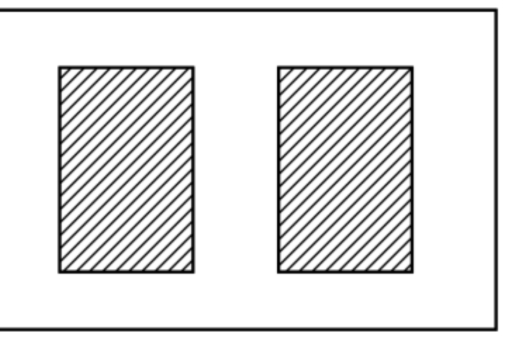
\includegraphics[width=0.34\textwidth]{figures/gao76_q20_poster.png}
\end{center}

\ifanswer
\solbegin
\stepm{(1)}{当 $x>0$ 时，$x+\dfrac1x\geqslant2\sqrt{x\times\dfrac1x}=2$，当且仅当 $x=\dfrac1x$，即 $x=1$ 取等号，}
\step{当 $x<0$ 时，$-x-\dfrac1x\geqslant2\sqrt{(-x)\times\dfrac1{-x}}=2$，所以 $x+\dfrac1x\leqslant-2$，}
\step{当且仅当 $-x=-\dfrac1x$，即 $x=-1$ 取等号，}
\step{综上所述，$x+\dfrac1x$ 的取值范围为 $(-\infty,-2]\cup[2,+\infty)$.}
\stepm{(2)}{设矩形栏目宽为 $x$，高为 $y$，则 $2xy=18000$，}
\step{所以 $S=(2x+36)(y+20)=2xy+36y+40x+720$}
% 原卷此行把 18720 写作 36720，照录（见文件头“原卷笔误/存疑”①）
\step{$=18000+36y+40x+720\geqslant18720+2\sqrt{36y\times40x}$}
\step{$=36720+2\sqrt{36\times40\times18000}=18720+7200=25920$，}
\step{当且仅当 $36y=40x$，即 $x=90$，$y=100$ 取等号，}
\step{所以海报的高为 $120\,\mathrm{cm}$ 与宽为 $216\,\mathrm{cm}$，可使矩形海报面积 $S$ 最小，}
\step{最小面积为 $25920$.}
\solend
\fi

\ansspace

\item 若实数 $x$、$y$、$m$ 满足 $|x-m|>|y-m|$，则称 $x$ 比 $y$ 远离 $m$.

（1）$0$ 比 $\dfrac12$ 远离 $2$ 吗？说明理由；

（2）若 $\dfrac1{2x-1}$ 比 $\dfrac12$ 远离 $1$，求实数 $x$ 的取值范围；

（3）若 $m\leqslant1$，$x+y=2$，试问：$x$ 与 $x^2+y^2$ 哪一个更远离 $m$，并说明理由.

\ifanswer
\solbegin
\stepm{(1)}{$0$ 比 $\dfrac12$ 远离 $2$，理由为：}
\step{由于 $|0-2|=2>\dfrac32=\left|\dfrac12-2\right|$，所以 $0$ 比 $\dfrac12$ 远离 $2$.}
\stepm{(2)}{由 $\dfrac1{2x-1}$ 比 $\dfrac12$ 远离 $1$，得 $\left|\dfrac1{2x-1}-1\right|>\left|\dfrac12-1\right|$，即 $\left|\dfrac1{2x-1}-1\right|>\dfrac12$，}
\step{则 $\dfrac1{2x-1}-1>\dfrac12$ 或 $\dfrac1{2x-1}-1<-\dfrac12$，整理得 $\dfrac1{2x-1}>\dfrac32$ 或 $\dfrac1{2x-1}<\dfrac12$，}
\step{因此 $0<2x-1<\dfrac23$ 或 $2x-1<0$ 或 $2x-1>2$，}
\step{解得 $\dfrac12<x<\dfrac56$ 或 $x<\dfrac12$ 或 $x>\dfrac32$，}
\step{所以 $x$ 的取值范围是 $\left(-\infty,\dfrac12\right)\cup\left(\dfrac12,\dfrac56\right)\cup\left(\dfrac32,+\infty\right)$.}
\stepm{(3)}{$x^2+y^2$ 比 $x$ 更远离 $m$，理由为：}
\step{由 $x^2+y^2\geqslant\dfrac{(x+y)^2}2=2\geqslant m$，得 $|x^2+y^2-m|=x^2+y^2-m$，}
\step{由 $x+y=2$，得 $x^2+y^2=x^2+(2-x)^2=2x^2-4x+4$，}
\step{于是 $|x^2+y^2-m|-|x-m|=2x^2-4x+4-m-|x-m|$，}
\step{当 $x\geqslant m$ 时，$|x^2+y^2-m|-|x-m|=2x^2-4x+4-m-(x-m)$}
\step{$=2\left(x-\dfrac54\right)^2+\dfrac78>0$，即 $|x^2+y^2-m|>|x-m|$；}
\step{当 $x<m$ 时，$|x^2+y^2-m|-|x-m|=2x^2-4x+4-m+(x-m)$}
\step{$=2\left(x-\dfrac34\right)^2+\dfrac{23}8-2m$，}
\step{由 $m\leqslant1$，得 $\dfrac{23}8-2m>0$，因此 $2\left(x-\dfrac34\right)^2+\dfrac{23}8-2m>0$，}
\step{即 $|x^2+y^2-m|>|x-m|$，}
\step{所以 $|x^2+y^2-m|>|x-m|$，即 $x^2+y^2$ 比 $x$ 更远离 $m$.}
\solend
\fi

\ansspace*[7]

\end{enumerate}

\end{document}
"
%
% 原始材料：微信公众号“魔都数学加油站”文章，连载“27学年高一76”；
% 原文标题“27学年高一76——2026-2027年上海市六十中学高一上10月月考”；
% 原文链接：https://mp.weixin.qq.com/s/GrKZjQrV1Xb0wy0BUuzAHw。
% 页面标注发布时间 2026-10-22 21:45（上海）。
% 正文为 10 张 PNG 页（`原图/高一76_六十中学_10月月考/01..10.png`）：
% 第 4、5、8、9 页为 4762×6735，其余 6 页为 2560×3620，均按页序读取。
% 10 页全为试卷正文页（卷首标题在第 1 页页顶，卷末第 21 题 (3) 解析止于第 10 页），
% 无封面页、目录页、二维码或宣传页。粉色斜排“魔都数学加油站”为卷面水印，未录入。
%
% 卷首标题：照卷面印作“2026-2027 年六十中学高一上 10 月月考”（黑体加粗一行）。
% 原卷年份区间用半角连字符，本稿按全稿惯例排 en dash；原卷无副标题。
%
% 篇幅与题号：原卷自第 3 题起编号（第 1、2 题不在本卷内）。填空题 3—12（10 题）、
% 选择题 13—16（4 题）、解答题 17—21（5 题），共 19 题。本稿沿用原节与原题号，
% 只改排为全稿统一的大节样式。
%
% 讲评版：原卷第 3、5 题只印【答案】（“$(0,1)$”“$a$、$b$ 都不能被 $3$ 整除”），
% 本稿只给 \ans{}；其余 17 题均印【解析】，用 \solbegin…\solend。四道选择题的作答
% 括号原卷即留空，答案写在解析末句“故选 C／B／C／D”，照录在解析内，不另提 \ans{}。
%
% 副标题：原卷未印副标题。本稿按“知识模块”口径标作“集合与常用逻辑用语、不等式”：
% 19 题中集合与常用逻辑用语 6 题（第 5、12、14、16、19 题及第 4 题的恒等变形），
% 不等式 13 题（第 3、6—11、13、15、17、18、20、21 题），两类均确有分量，故并标。
% 口径同 高一63、高一68—75。
%
% 与原卷的排版差异：
%   ① 原卷每题下直接印【答案】/【解析】，本稿按全稿惯例将答案与解析置于答案版；
%   ② 原卷未印副标题，本稿按“知识模块”口径补出；
%   ③ 原卷填空横线约四个字宽，本稿按全稿惯例统一排 \blankline[4.4em]；
%   ④ 原卷数集记号排斜体 $R$、$N$（第 4、6、7、8、11、12、14、15、19、20 题），本稿
%      按全稿惯例改用 $\R$、$\N$（同 高一68—75）；第 7、19、20 题的“解集为 $\R$”同此；
%   ⑤ 原卷句末标点多为西文句点，均逐处照录；
%   ⑥ 第 17—21 题的子问原卷印作“（1）…（2）…”，本稿按 高一69—75 成例用行内
%      “（1）（2）（3）”段，解析中的子问标号用 \stepm{(1)}{…}；
%   ⑦ 每道解答题原卷未留作答空白，本稿按全稿惯例加 \ansspace（末题用 \ansspace*）；
%   ⑧ 选择题的作答括号原卷排半角“(    )”，本稿按全稿惯例排 \mbox{（\quad）}；
%      选项行排照原卷——第 13、14、15、16 题一行两条、分两行排（本稿按原卷分行）；
%   ⑨ 第 10、11、17—21 题解析中的不等式组／方程组，原卷均排作“{”连接的多行式，
%      本稿按全稿惯例排 cases；
%   ⑩ 第 14 题题干右侧有一幅韦恩图（全集矩形内含 A、B 两圆，B 涂灰）：本稿按原卷
%      截图裁取（`figures/gao76_q14_venn.png`，由第 5 页原图裁出、去除粉色水印后转
%      灰度，未放大），放在题干之后、选项之前，仅答案版出；
%   ⑪ 第 20 题 (2) 题干右侧有一幅示意图（大矩形内两个斜线阴影小矩形）：本稿按原卷
%      截图裁取（`figures/gao76_q20_poster.png`，由第 8 页原图裁出、去除粉色水印后转
%      灰度，未放大），放在该小题文字之后，仅答案版出。
%
% 原卷笔误/存疑（均照录未改，正文对应处另有 % 注）：
%   ① 第 20 题 (2) 解析第 3 行把 $2xy+720$ 写成 $36720$（实为 $18000+720=18720$），
%      同式下一行又写回 $18720$，前后不一致；原卷如此，照录未改。
%   ② 第 14 题的韦恩图阴影是把整个 $B$ 圆（含 $A\cap B$ 部分）涂灰，而解析按
%      $\overline{A\cap B}$ 求解，二者不一致；原卷图文如此，照录未改。
%
% 行数核对：逐题数 \step/\stepm 条数与原卷【解析】印刷行数，17 题逐一相符，
% 合计 118 条 / 118 行（Q4：3；Q6：4；Q7：1；Q8：6；Q9：3；Q10：7；Q11：4；
% Q12：16；Q13：1；Q14：3；Q15：7；Q16：10；Q17：12；Q18：6；Q19：6；Q20：11；
% Q21：18）。另第 3、5 题只印【答案】，各提 \ans{}，不计入 \step 账。
%
% 插图：第 14 题题干的韦恩图、第 20 题 (2) 的示意图，见上⑩⑪；其余题干无配图。
%
\documentclass[a4paper,11pt]{article}
\usepackage{common}

\begin{document}

\examtitlest[3]{2026--2027 年六十中学高一上 10 月月考}{集合与常用逻辑用语、不等式}

\bigsec{一、填空题}

\begin{enumerate}
\setcounter{enumi}{2}

\item 不等式 $\dfrac{x}{1-x}>0$ 的解集是\blankline[4.4em].

\ifanswer
\ans{$(0,1)$}
\fi

\item 已知 $2x^2+x+1=a(x+1)^2+b(x+1)+2$，对 $x\in\R$ 恒成立，$ab=$\blankline[4.4em].

\ifanswer
\solbegin
\step{若 $2x^2+x+1=a(x+1)^2+b(x+1)+2$ 对 $x\in\R$ 恒成立，}
\step{即 $2x^2+x+1=ax^2+(2a+b)x+a+b+2$ 对 $x\in\R$ 恒成立，}
\step{必有 $\begin{cases}a=2\\ 2a+b=1\\ a+b+2=1\end{cases}$，解得 $a=2$，$b=-3$，所以 $ab=-6$.}
\solend
\fi

\item 利用反证法证明命题：“如果 $a$、$b\in\N$，$ab$ 可被 $3$ 整除，那么 $a$、$b$ 中至少有一个能被 $3$ 整除”时，假设的内容应是\blankline[4.4em].

\ifanswer
\ans{$a$、$b$ 都不能被 $3$ 整除}
\fi

\item 已知 $x\in\R$，方程 $|x+1|+|2-x|=3$ 的解集为\blankline[4.4em].

\ifanswer
\solbegin
\step{当 $x<-1$ 时，则 $|x+1|+|2-x|=-x-1+2-x=1-2x>3$；}
\step{当 $-1\leqslant x\leqslant2$ 时，则 $|x+1|+|2-x|=x+1+2-x=3$；}
\step{当 $x>2$ 时，则 $|x+1|+|2-x|=x+1+x-2=2x-1>3$.}
\step{综上所述，原方程的解集为 $[-1,2]$.}
\solend
\fi

\item 若关于 $x$ 的不等式 $x^2+kx+1\geqslant0$ 的解集为 $\R$，则实数 $k$ 的取值范围是\blankline[4.4em].

\ifanswer
\solbegin
\step{$\Delta=k^2-4\leqslant0\Rightarrow-2\leqslant k\leqslant2$，所以实数 $k$ 的取值范围是 $[-2,2]$.}
\solend
\fi

\item 已知 $a$、$b\in\R$，且 $ab>0$，则下列不等式中，恒成立的序号是\blankline[4.4em].

① $a^2+b^2>2ab$；② $a+b\geqslant2\sqrt{ab}$；③ $\dfrac1a+\dfrac1b>\dfrac2{\sqrt{ab}}$；④ $\dfrac ba+\dfrac ab\geqslant2$.

\ifanswer
\solbegin
\step{因为 $a^2+b^2\geqslant2ab$ 对于 $a$、$b\in\R$ 恒成立，当且仅当 $a=b$ 时取等号，}
\step{所以①错误；}
\step{对于②，③，显然 $a<0$，$b<0$ 时，不等式均不成立，即②和③错误；}
\step{对于④，因为 $ab>0$，所以 $\dfrac ba>0,\dfrac ab>0$，}
\step{由基本不等式得 $\dfrac ba+\dfrac ab\geqslant2\sqrt{\dfrac ba\cdot\dfrac ab}=2$，即④正确.}
\step{故正确的是④.}
\solend
\fi

\item 已知正实数 $m$、$n$ 满足 $m+\dfrac2n=1$，则 $\dfrac1m+2n$ 的最小值为\blankline[4.4em].

\ifanswer
\solbegin
\step{$\dfrac1m+2n=\left(m+\dfrac2n\right)\left(\dfrac1m+2n\right)=5+2mn+\dfrac2{mn}$，}
\step{因为 $mn>0$，所以 $2mn+\dfrac2{mn}\geqslant2\sqrt{2mn\cdot\dfrac2{mn}}=4$，}
\step{当且仅当 $2mn=\dfrac2{mn}$，即 $m=\dfrac13$，$n=3$ 时取等号，所以 $\dfrac1m+2n$ 的最小值为 $9$.}
\solend
\fi

\item 若关于 $x$ 的不等式组 $\begin{cases}3x+1>0\\ x+\dfrac1a\leqslant2\end{cases}$ 恰好有两个整数解，则实数 $a$ 的取值范围为\blankline[4.4em].

\ifanswer
\solbegin
\step{由 $3x+1>0$ 得 $x>-\dfrac13$；若 $a<0$，则 $\dfrac1a<0$，由 $x+\dfrac1a\leqslant2$ 得 $x\leqslant2-\dfrac1a>2$，}
\step{则解集 $\left(-\dfrac13,2-\dfrac1a\right]$ 必同时含有整数 $0$、$1$、$2$，不合题意；}
\step{又 $a=0$ 使 $\dfrac1a$ 无意义，故 $a>0$；}
\step{此时原不等式组的解集为 $\left(-\dfrac13,2-\dfrac1a\right]$，}
\step{其中大于 $-\dfrac13$ 的整数依次为 $0$，$1$，$2$，$\cdots$，}
\step{恰有两个整数解即解集只含 $0$ 与 $1$，故 $1\leqslant2-\dfrac1a<2$，即 $\dfrac1a\leqslant1$ 且 $\dfrac1a>0$，}
\step{结合 $a>0$，解得 $a\geqslant1$.}
\solend
\fi

\item 已知 $a\in\R$，若关于 $x$ 的方程 $x^2+ax+a^2-8=0$ 有两个实根 $x_1$、$x_2$，且 $\dfrac1{x_1}+\dfrac1{x_2}=-\dfrac12$，则 $a$ 的值为\blankline[4.4em].

\ifanswer
\solbegin
\step{由题意得 $\Delta=a^2-4(a^2-8)=32-3a^2\geqslant0$，解得 $a^2\leqslant\dfrac{32}3$，}
\step{由韦达定理得 $x_1+x_2=-a$，$x_1x_2=a^2-8$，}
\step{则 $\dfrac1{x_1}+\dfrac1{x_2}=\dfrac{x_1+x_2}{x_1x_2}=\dfrac{-a}{a^2-8}=-\dfrac12$，即 $a^2-2a-8=(a-4)(a+2)=0$，}
\step{解得 $a=4$ 或 $a=-2$，又 $a^2\leqslant\dfrac{32}3$，则 $a=-2$.}
\solend
\fi

\item 已知有限集 $A=\{a_1,a_2,\cdots,a_n\}(n\geqslant2,n\in\N)$，若 $A$ 中元素 $a_i(i=1,2,\cdots,n)$ 满足 $a_1+a_2+\cdots+a_n=a_1\times a_2\times\cdots\times a_n$，就称 $A$ 为“完美集”，以下四个命题：

①集合 $\{-1-\sqrt3,-1+\sqrt3\}$ 不是“完美集”；

②若 $a_1$、$a_2$ 是两个不同的正数，且 $\{a_1,a_2\}$ 是“完美集”，则 $a_1$、$a_2$ 至少有一个大于 $2$；

③二元“完美集”有无穷多个；

④若 $a_i$ 均为正整数，则“完美集”$A$ 有且只有一个，且 $n=3$.

其中，真命题的序号是\blankline[4.4em].

\ifanswer
\solbegin
\step{对于①选项：$(-1-\sqrt3)+(-1+\sqrt3)=-2$，$(-1-\sqrt3)\times(-1+\sqrt3)=-2$，}
\step{故 $(-1-\sqrt3)+(-1+\sqrt3)=(-1-\sqrt3)\times(-1+\sqrt3)$，}
\step{所以集合 $\{-1-\sqrt3,-1+\sqrt3\}$ 是“完美集”，故①错误；}
\step{对于②选项：集合 $\{a_1,a_2\}$ 是“完美集”，设 $a_1+a_2=a_1a_2=t>0$，}
\step{则 $a_1$、$a_2$ 可以看成一元二次方程 $x^2-tx+t=0$ 的两正根，则 $\Delta=t^2-4t>0$，}
\step{解得 $t<0$（舍）或 $t>4$，即 $a_1a_2>4$，所以至少有一个大于 $2$，故②正确；}
\step{对于③选项：由②得一元二次方程 $x^2-tx+t=0$ 当 $t$ 取不同值时，}
\step{$a_1$、$a_2$ 的值是不同的，因而二元“完美集”有无穷多个，故③正确；}
\step{对于④选项：设 $a_1<a_2<a_3<\cdots<a_n$，}
\step{则 $a_1\times a_2\times\cdots\times a_n=a_1+a_2+\cdots+a_n<na_n$，}
\step{所以 $a_1\times a_2\times\cdots\times a_{n-1}<n$，又 $a_i\in\N^*$，所以 $n\leqslant3$，}
\step{当 $n=2$ 时，$a_1<2$，则 $a_1=1$，$a_1a_2\neq a_1+a_2$，不合题意，}
\step{当 $n=3$ 时，$a_1a_2<3$，所以只能是 $a_1=1$，$a_2=2$，}
\step{由 $a_1+a_2+a_3=a_1a_2a_3$，代入解得 $a_3=3$，所以此时“完美集”只有一个，}
\step{为 $\{1,2,3\}$，故④正确.}
\step{故正确的是②③④.}
\solend
\fi

\end{enumerate}

\bigsec{二、选择题}

\begin{enumerate}
\setcounter{enumi}{12}

\item 已知 $x$、$y\in\R$，则“$xy\geqslant0$”是“$xy=|xy|$”的\mbox{（\quad）}

\keepwithprev
A. 充分非必要条件\qquad B. 必要非充分条件

C. 充要条件\qquad D. 既非充分也非必要条件

\ifanswer
\solbegin
\step{$xy\geqslant0\Leftrightarrow xy=|xy|$，故“$xy\geqslant0$”是“$xy=|xy|$”的充要条件. 故选 $C$.}
\solend
\fi

\needvspace{22\baselineskip}
\item 已知全集 $U=\R$，集合 $A=\{x\mid x<-1\text{ 或 }x>4\}$，$B=\{x\mid x^2-x-6\leqslant0\}$，则阴影部分表示的集合为\mbox{（\quad）}

\begin{center}
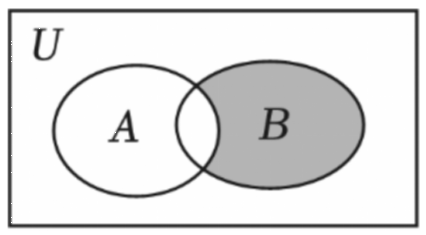
\includegraphics[width=0.26\textwidth]{figures/gao76_q14_venn.png}
\end{center}

\keepwithprev
A. $\{x\mid-2\leqslant x<4\}$\qquad B. $\{x\mid-1\leqslant x\leqslant3\}$

C. $\{x\mid x\leqslant3\text{ 或 }x\geqslant4\}$\qquad D. $\{x\mid-2\leqslant x\leqslant4\}$

\ifanswer
\solbegin
\step{全集 $U=\R$，集合 $A=\{x\mid x<-1\text{ 或 }x>4\}$，}
\step{$B=\{x\mid x^2-x-6\leqslant0\}=\{x\mid-2\leqslant x\leqslant3\}$，故 $A\cap B=\{x\mid-2\leqslant x<-1\}$，}
\step{故阴影部分表示的集合为 $\overline{A\cap B}=\{x\mid-1\leqslant x\leqslant3\}$. 故选 $B$.}
\solend
\fi

\item 设 $a$、$b$、$c\in\R$，给出下列命题：①若 $a>b$，则 $a^2>b^2$，②“$a>b$”是“$a^3>b^3$”的充要条件，③若 $a^2>b^2$，则 $|a|>|b|$，④若 $\dfrac ab>1$，则 $a>b$，⑤若 $a>b$，$c\neq0$，则 $\dfrac a{c^2}>\dfrac b{c^2}$，其中真命题的个数是\mbox{（\quad）}

\keepwithprev
A. $1$ 个\qquad B. $2$ 个\qquad C. $3$ 个\qquad D. $4$ 个

\ifanswer
\solbegin
\step{对于①，取 $a=2$，$b=-2$，满足 $a>b$，而 $a^2=b^2$，故为假命题；}
\step{对于②，$a>b\Leftrightarrow a^3-b^3=(a-b)(a^2+ab+b^2)=(a-b)\left[\left(a+\dfrac12b\right)^2+\dfrac34b^2\right]>0$}
\step{$\Leftrightarrow a^3>b^3$，故为真命题；}
\step{对于③，$a^2>b^2\Leftrightarrow|a|^2>|b|^2\Leftrightarrow|a|>|b|$，故为真命题；}
\step{对于④，取 $a=-2$，$b=-1$，满足 $\dfrac ab>1$，而 $a<b$，故为假命题；}
\step{对于⑤，由题意得 $c^2>0$，由 $a>b$，则 $\dfrac a{c^2}>\dfrac b{c^2}$，故为真命题.}
\step{故选 $C$.}
\solend
\fi

\item 已知关于 $x$ 的两个一元二次不等式 $a_1x^2+b_1x+c_1>0$，$a_2x^2+b_2x+c_2>0$ 的解集分别为 $A$、$B$，其中 $a_i$、$b_i$、$c_i(i=1,2)$ 为常数且不为零，则“$\dfrac{a_1}{a_2}=\dfrac{b_1}{b_2}=\dfrac{c_1}{c_2}$”是“$A=B$”\mbox{（\quad）}

\keepwithprev
A. 充分不必要条件\qquad B. 必要不充分条件

C. 充要条件\qquad D. 既不充分也不必要条件

\ifanswer
\solbegin
\step{设 $\dfrac{a_1}{a_2}=\dfrac{b_1}{b_2}=\dfrac{c_1}{c_2}=\lambda$，}
\step{①当 $\lambda>0$ 时，则 $a_1=\lambda a_2$，$b_1=\lambda b_2$，$c_1=\lambda c_2$，}
\step{$a_1x^2+b_1x+c_1>0\Leftrightarrow\lambda a_2x^2+\lambda b_2x+\lambda c_2>0\Leftrightarrow a_2x^2+b_2x+c_2>0$，}
\step{所以 $A=B$，}
\step{②当 $\lambda<0$ 时，则 $a_1=\lambda a_2$，$b_1=\lambda b_2$，$c_1=\lambda c_2$，}
\step{$a_1x^2+b_1x+c_1>0\Leftrightarrow\lambda a_2x^2+\lambda b_2x+\lambda c_2>0\Leftrightarrow a_2x^2+b_2x+c_2<0$，}
\step{所以 $A\neq B$，充分性不成立，}
\step{当 $A=B=\R$ 时，则 $\Delta<0$ 且 $a_1$、$a_2>0$，$\dfrac{a_1}{a_2}=\dfrac{b_1}{b_2}=\dfrac{c_1}{c_2}$ 不一定成立，}
\step{必要性不成立.}
\step{所以 $\dfrac{a_1}{a_2}=\dfrac{b_1}{b_2}=\dfrac{c_1}{c_2}$ 是 $A=B$ 的既不充分也不必要条件，故选 $D$.}
\solend
\fi

\end{enumerate}

\bigsec{三、解答题}

\begin{enumerate}
\setcounter{enumi}{16}

\item 求下列关于 $x$ 的不等式（组）的解集.

（1）$\begin{cases}9x^2-6x-24>0\\ \dfrac{x+3}{x-1}>2\end{cases}$；

（2）$|2x+1|-|2-x|>2$.

\ifanswer
\solbegin
\stepm{(1)}{不等式 $\dfrac{x+3}{x-1}>2$ 可化为 $\dfrac{x+3}{x-1}-2>0$，}
\step{即 $\dfrac{-x+5}{x-1}>0$，即 $(x-1)(x-5)<0$，解得 $1<x<5$，}
\step{不等式 $9x^2-6x-24>0$ 可化为 $(3x+4)(x-2)>0$，}
\step{解得 $x<-\dfrac43$ 或 $x>2$，}
\step{所以不等式的解集为 $(2,5)$.}
\stepm{(2)}{当 $x\leqslant-\dfrac12$ 时，$|2x+1|-|2-x|>2$ 等价于 $-2x-1-(2-x)>2$，}
\step{解得 $x<-5$，所以 $x<-5$，}
\step{当 $-\dfrac12<x<2$ 时，$|2x+1|-|2-x|>2$ 等价于 $2x+1-(2-x)>2$，}
\step{解得 $x>1$，所以 $1<x<2$，}
\step{当 $x\geqslant2$ 时，$|2x+1|-|2-x|>2$ 等价于 $2x+1-(x-2)>2$，}
\step{解得 $x>-1$，所以 $x\geqslant2$，}
\step{综上，$|2x+1|-|2-x|>2$ 的解集为 $(-\infty,-5)\cup(1,+\infty)$.}
\solend
\fi

\ansspace

\item 设 $m$ 为实数，求关于 $x$ 与 $y$ 的二元一次方程组 $\begin{cases}y=x+m\\ mx-y=4\end{cases}$ 的解集.

\ifanswer
\solbegin
\step{消去 $y$ 得 $(m-1)x=m+4$，}
\step{当 $m-1=0$，即 $m=1$ 时，$0=5$ 不成立，则 $x$ 无解，原方程组的解集为 $\varnothing$；}
\step{当 $m-1\neq0$，即 $m\neq1$ 时，则 $x=\dfrac{m+4}{m-1}$，$y=\dfrac{m+4}{m-1}+m=\dfrac{m^2+4}{m-1}$，}
\step{原方程组的解集为 $\left\{\left(\dfrac{m+4}{m-1},\dfrac{m^2+4}{m-1}\right)\right\}$.}
\step{综上所述，当 $m=1$ 时，方程组的解集为 $\varnothing$；}
\step{当 $m\neq1$ 时，方程组的解集为 $\left\{\left(\dfrac{m+4}{m-1},\dfrac{m^2+4}{m-1}\right)\right\}$.}
\solend
\fi

\ansspace

\item 已知集合 $A=\{x\mid-2\leqslant x-1\leqslant5\}$，集合 $B=\{x\mid m+1\leqslant x\leqslant2m-1\}(m\in\R)$.

（1）若 $m=4$，全集 $U=\R$，求 $A\cap B$；

（2）设命题 $p:x\in A$；命题 $q:x\in B$，若命题 $p$ 是命题 $q$ 的必要不充分条件，求实数 $m$ 的取值范围.

\ifanswer
\solbegin
\stepm{(1)}{由题意得 $A=\{x\mid-2\leqslant x-1\leqslant5\}=\{x\mid-1\leqslant x\leqslant6\}$，}
\step{当 $m=4$ 时，$B=\{x\mid5\leqslant x\leqslant7\}$，$A\cap B=\{x\mid5\leqslant x\leqslant6\}$；}
\stepm{(2)}{因为命题 $p$ 是命题 $q$ 的必要不充分条件，所以集合 $B$ 是集合 $A$ 的真子集，}
\step{当 $B=\varnothing$ 时，$m+1>2m-1$，解得 $m<2$，}
\step{当 $B\neq\varnothing$ 时，$\begin{cases}m+1\leqslant2m-1\\ m+1\geqslant-1\\ 2m-1\leqslant6\end{cases}$（等号不能同时成立），解得 $2\leqslant m\leqslant\dfrac72$，}
\step{综上所述，实数 $m$ 的取值范围为 $\left(-\infty,\dfrac72\right]$.}
\solend
\fi

\ansspace

\item （1）已知实数 $x\neq0$，求 $x+\dfrac1x$ 的取值范围；

（2）如图，要设计一张矩形海报，该海报含有大小相等的左右两个矩形栏目（即图中阴影部分），这两栏的面积之和为 $18000\,\mathrm{cm}^2$，四周空白的宽度为 $10\,\mathrm{cm}$，两栏之间的中缝空白的宽度为 $16\,\mathrm{cm}$，怎样确定海报的高与宽的尺寸（单位：$\mathrm{cm}$），能使矩形海报面积 $S$ 最小？最小面积是多少？

\begin{center}
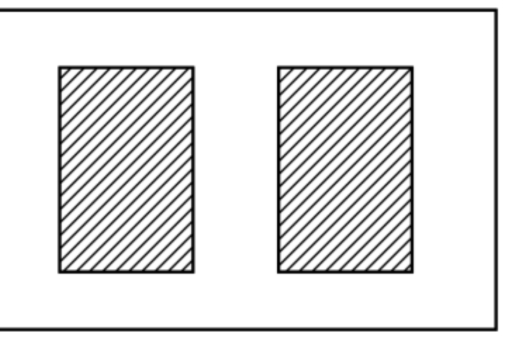
\includegraphics[width=0.34\textwidth]{figures/gao76_q20_poster.png}
\end{center}

\ifanswer
\solbegin
\stepm{(1)}{当 $x>0$ 时，$x+\dfrac1x\geqslant2\sqrt{x\times\dfrac1x}=2$，当且仅当 $x=\dfrac1x$，即 $x=1$ 取等号，}
\step{当 $x<0$ 时，$-x-\dfrac1x\geqslant2\sqrt{(-x)\times\dfrac1{-x}}=2$，所以 $x+\dfrac1x\leqslant-2$，}
\step{当且仅当 $-x=-\dfrac1x$，即 $x=-1$ 取等号，}
\step{综上所述，$x+\dfrac1x$ 的取值范围为 $(-\infty,-2]\cup[2,+\infty)$.}
\stepm{(2)}{设矩形栏目宽为 $x$，高为 $y$，则 $2xy=18000$，}
\step{所以 $S=(2x+36)(y+20)=2xy+36y+40x+720$}
% 原卷此行把 18720 写作 36720，照录（见文件头“原卷笔误/存疑”①）
\step{$=18000+36y+40x+720\geqslant18720+2\sqrt{36y\times40x}$}
\step{$=36720+2\sqrt{36\times40\times18000}=18720+7200=25920$，}
\step{当且仅当 $36y=40x$，即 $x=90$，$y=100$ 取等号，}
\step{所以海报的高为 $120\,\mathrm{cm}$ 与宽为 $216\,\mathrm{cm}$，可使矩形海报面积 $S$ 最小，}
\step{最小面积为 $25920$.}
\solend
\fi

\ansspace

\item 若实数 $x$、$y$、$m$ 满足 $|x-m|>|y-m|$，则称 $x$ 比 $y$ 远离 $m$.

（1）$0$ 比 $\dfrac12$ 远离 $2$ 吗？说明理由；

（2）若 $\dfrac1{2x-1}$ 比 $\dfrac12$ 远离 $1$，求实数 $x$ 的取值范围；

（3）若 $m\leqslant1$，$x+y=2$，试问：$x$ 与 $x^2+y^2$ 哪一个更远离 $m$，并说明理由.

\ifanswer
\solbegin
\stepm{(1)}{$0$ 比 $\dfrac12$ 远离 $2$，理由为：}
\step{由于 $|0-2|=2>\dfrac32=\left|\dfrac12-2\right|$，所以 $0$ 比 $\dfrac12$ 远离 $2$.}
\stepm{(2)}{由 $\dfrac1{2x-1}$ 比 $\dfrac12$ 远离 $1$，得 $\left|\dfrac1{2x-1}-1\right|>\left|\dfrac12-1\right|$，即 $\left|\dfrac1{2x-1}-1\right|>\dfrac12$，}
\step{则 $\dfrac1{2x-1}-1>\dfrac12$ 或 $\dfrac1{2x-1}-1<-\dfrac12$，整理得 $\dfrac1{2x-1}>\dfrac32$ 或 $\dfrac1{2x-1}<\dfrac12$，}
\step{因此 $0<2x-1<\dfrac23$ 或 $2x-1<0$ 或 $2x-1>2$，}
\step{解得 $\dfrac12<x<\dfrac56$ 或 $x<\dfrac12$ 或 $x>\dfrac32$，}
\step{所以 $x$ 的取值范围是 $\left(-\infty,\dfrac12\right)\cup\left(\dfrac12,\dfrac56\right)\cup\left(\dfrac32,+\infty\right)$.}
\stepm{(3)}{$x^2+y^2$ 比 $x$ 更远离 $m$，理由为：}
\step{由 $x^2+y^2\geqslant\dfrac{(x+y)^2}2=2\geqslant m$，得 $|x^2+y^2-m|=x^2+y^2-m$，}
\step{由 $x+y=2$，得 $x^2+y^2=x^2+(2-x)^2=2x^2-4x+4$，}
\step{于是 $|x^2+y^2-m|-|x-m|=2x^2-4x+4-m-|x-m|$，}
\step{当 $x\geqslant m$ 时，$|x^2+y^2-m|-|x-m|=2x^2-4x+4-m-(x-m)$}
\step{$=2\left(x-\dfrac54\right)^2+\dfrac78>0$，即 $|x^2+y^2-m|>|x-m|$；}
\step{当 $x<m$ 时，$|x^2+y^2-m|-|x-m|=2x^2-4x+4-m+(x-m)$}
\step{$=2\left(x-\dfrac34\right)^2+\dfrac{23}8-2m$，}
\step{由 $m\leqslant1$，得 $\dfrac{23}8-2m>0$，因此 $2\left(x-\dfrac34\right)^2+\dfrac{23}8-2m>0$，}
\step{即 $|x^2+y^2-m|>|x-m|$，}
\step{所以 $|x^2+y^2-m|>|x-m|$，即 $x^2+y^2$ 比 $x$ 更远离 $m$.}
\solend
\fi

\ansspace*[7]

\end{enumerate}

\end{document}
